\documentclass[a4paper , 12pt]{book}
\usepackage[utf8]{inputenc}
\usepackage[english]{babel}
\usepackage{mathtools}
\usepackage{listings}
\usepackage{xcolor}
\usepackage{hyperref}
\usepackage{graphicx}
\usepackage{float}
\usepackage{gensymb}
\usepackage{textcomp} % This fixes the problem with single quotes in Python
\usepackage{sidecap} % caption to the side of figure
\usepackage{siunitx} % SI units
\usepackage{wasysym}
\graphicspath{{./figures/}}

\hypersetup{
    colorlinks=true,
    linkcolor=blue,
    filecolor=magenta,      
    urlcolor=cyan,
    pdftitle={Sharelatex Example},
    %bookmarks=true,
    pdfpagemode=FullScreen,
    }
 
\definecolor{codegreen}{rgb}{0,0.6,0}
\definecolor{codegray}{rgb}{0.5,0.5,0.5}
\definecolor{codepurple}{rgb}{0.58,0,0.82}
\definecolor{backcolour}{gray}{0.90}
\definecolor{light-gray}{gray}{0.95}
 
\lstdefinestyle{mystyle}{
    backgroundcolor=\color{backcolour},   
    commentstyle=\color{codegreen},
    keywordstyle=\color{magenta},
    numberstyle=\tiny\color{codegray},
    stringstyle=\color{codepurple},
    basicstyle=\ttfamily\footnotesize,
    breakatwhitespace=false,         
    breaklines=true,                 
    captionpos=b,                    
    keepspaces=true,                 
    numbers=left,                    
    numbersep=5pt,                  
    showspaces=false,                
    showstringspaces=false,
    showtabs=false,                  
    tabsize=2
}

% Better inline directory listings
\newcommand{\code}[1]{\colorbox{light-gray}{\texttt{#1}}}

\begin{document}
 \pagenumbering{gobble}

\lstset{style=mystyle}
\lstset{language=Python,upquote=true} % This fixes the problem with single quotes in Python
\title{Computational Geosciences}
\author{An educational project funded by the \\ \\ Faculty of Science and Technology \\ \\ University of Stavanger, Norway \\ \\ \\ \\ \\ \\ Editor: Nestor Cardozo \\ \\ \\ \\ \\ \\}

\setlength{\parindent}{0pt}
\setlength{\parskip}{1em}
\renewcommand{\baselinestretch}{1.}

\maketitle
\pagenumbering{arabic}

% PREFACE
\section*{Preface}

Welcome to the Computational Geosciences resource at the University of Stavanger, Norway (UiS). Computational Geosciences is not a new subject. A course in Computational Geology was offered at the University of South Florida for the first time in 1996 (Vacher, 2000). Computational Geosciences makes connections between mathematics, computation and geology. It promotes a mathematical problem-solving disposition (Vacher, 2000). 

This resource is designed based on the same principles and with emphasis on problem-solving. However, the access to data and the tools to visualize and analize data have improved tremendously over the last 20 years. Today, a geologist carrying a mobile device in the field has access to a collection of sensors collecting data in real time (magnetometer, accelerometers, gravity, GPS, etc.), and accurate databases of topography, aerial photos, and satellite imagery. Such information not only supports the geologist in the field, but also allows her to test hypotheses and take decisions. Computation is greatly facilitated by high-level programming languages (e.g. Matlab and Python) that focus on solving and visualizing problems, rather than on coding details. The digital era is here, and to analyze the large number of data associated with it, we need math and computing. 

To develop this resource, we put together an interesting group of faculty from the Departments of Energy Resources (IER) and Mechanical and Structural Engineering (IMBM) at the University of Stavanger, with expertise in Geographic Information Science (GIS, Lisa Watson, IER), Geophysics (Wiktor Weibull, IER), Structural Geology (Nestor Cardozo, IER), and Fluid Mechanics (Knut Giljarhus, IMBM). Postdoc David Oakley (IER) also contributed to the resource. Master students from Computational Engineering (Angela Hoch), Offshore Engineering (Adham Amer), and Geosciences (Vania Mansoor and Linda Olsen) were instrumental. They wrote our scattered code into functions and notebooks, solved the exercise problems, and helped editing the resource in \href {https://www.overleaf.com}{Overleaf}. 

Python is the programming language of choice. The resource consists of ten chapters covering an introduction to computation in Geosciences and Python (chapter 1), understanding location (chapter 2), orientation and display of geological features (chapter 3), coordinate systems and vectors (chapter 4), coordinate transformations (chapter 5), tensors (chapter 6), stress (chapter 7), strain (chapter 8), elasticity (chapter 9), and the inverse problem (chapter 10). Each chapter describes the basic theory before going directly into applications and problems. Exercises at the end of each chapter are essential to master the material. These exercises are not trivial.

Much of the material is based on the book Structural Geology Algorithms: Vectors and Tensors (Allmendinger et al., 2012), and the lab manual: Modern Structural Practice (Allmendinger, 2020). However, we have also included additional GIS and Geophysics topics. The resource is focused on our areas of expertise, but the material can be applied to other areas.

You can download or subscribe to changes in the resource using its \href{https://github.com/nfcd/compGeo}{git repository}. We hope you enjoy this resource and learn from it, as well as use it for teaching and research. We also hope to spark enough interest for users to contribute to the resource with additional material. Finally, we are grateful to the Faculty of Science and Technology at the University of Stavanger for sponsoring this project. We also like to thank Artem Mostalenko (Saint Petersburg U.) and Rustam Zaitov for careful review of the resource and code suggestions.

\section*{Accessing the resource material}

The best way to access the resource is by cloning or downloading its \href{https://github.com/nfcd/compGeo}{git repository}. This repository contains a \href{https://github.com/nfcd/compGeo/blob/master/compGeo.pdf}{pdf of this book} and a folder called \href{https://github.com/nfcd/compGeo/blob/master/source}{source} with the \href{https://github.com/nfcd/compGeo/blob/master/source/notebooks}{notebooks}, \href{https://github.com/nfcd/compGeo/blob/master/source/functions}{functions} and \href{https://github.com/nfcd/compGeo/blob/master/source/data}{data} in their corresponding folders. The notebooks follow this directory structure. We recommend you use the same structure when running them.

\section*{References}

Allmendinger, R.W., Cardozo, N. and Fisher, D.M. 2012. Structural Geology Algorithms: Vectors and Tensors. Cambridge University Press.

Allmendinger, R.W. 2020. Modern Structural Practice: A structural geology laboratory manual for the 21st century. [\href{https://www.rickallmendinger.net/download}{Online}]. [Accessed March, 2021].

Vacher, H.L. 2000. A Course in Geological-Mathematical Problem Solving. Journal of Geoscience Education 48, 478-481.

% TABLE OF CONTENTS
\tableofcontents

% CHAPTER 1: COMPUTATION IN GEOSCIENCES
\chapter{Computation in Geosciences}

% SECTION: SOLVING PROBLEMS BY COMPUTATION
\section{Solving problems by computation}

Geology is an interpretive and historical science (Frodeman, 1995). We observe, collect, analyze, and interpret data (what) to tell a story (why). To collect data, we need to take measurements. All measurements have some uncertainty, and therefore uncertainty and error propagation are important in geosciences, and they are a recurring topic in this resource.

For the last 50 years or more, the methods geoscientists have used to visualize, analyze and interpret data are mostly graphical. For example, in structural geology, students typically learn two types of graphical constructions: orthographic and  spherical projections (stereonets) (Ragan, 2009). Although these methods are great to visualize and solve geometrical problems in three-dimensions, they are not amenable to computation, and therefore applying these methods to large datasets with thousands of entries is impractical. Plane and spherical trigonometry allow deriving formulas (e.g. apparent dip formula) for computation (Ragan, 2009). However, these formulas give little insight about the problems. They are just formulas associated with complex geometric constructions, which bear no relation to each other, and which are difficult to combine to solve more complicated problems.

It turns out that many of the most interesting problems in geosciences can be solved using linear algebra, and vectors and tensors (Allmendinger et al., 2012). Linear algebra also happens to be the language of computation. The main purpose of this resource is to show how to solve problems in geosciences using computation. There are several advantages of following this approach. It will enhance your mathematical and computational skills, as well as promote your geological-mathematical problem solving disposition. In today’s digital age, these skills are very useful.

\section{Why Python?}

The choice of programming language is important. While computer languages such as C or C++ are ideal to work with large datasets and computer-intensive operations, they involve a steep learning curve associated with their syntax, compilation, and execution (Jacobs et al., 2016). These coding details have little to do with the problem-solving approach of this resource. Interpretive languages such as Python, R or Matlab are a better choice because of their simpler syntax, and the interpretation and execution of commands as they are called (no need for compilation). In addition, these languages have access to an integrated development environment (IDE) that facilitates writing and debugging programs, and to many standard libraries that perform advanced tasks such as matrix operations and data visualization. Thus, Python, R or Matlab are “scientific packages” rather than just programming languages.

In this resource, the language of choice is Python. Besides the reasons above, Python has the following advantages:
\begin{itemize}
  \item Python can be learned quickly. It typically involves less code than other languages and its syntax is easier to read.
  \item Python comes with robust standard libraries for arrays and mathematical functions (NumPy), visualization (Pyplot), and scientific computing (SciPy).
  \item As of December 2022, Python is the most popular programming language followed by C, C++, and Java (\href {https://tiobe.com/tiobe-index/}{TIOBE index}), with a large base of developers and users. It is used by every major technology company and it is almost a skill you must have in your CV to land a job as a geoscientist.
  \item Because of its large developers base, Python has access to a large amount of external libraries, including several libraries for geosciences. We make use of some of these libraries in this resource.
  \item Python can be installed easily through a single distribution that includes all the standard libraries and provides access to external libraries (see next section).
  \item Last but not least, Python is free and open source. This is probably why Python is more popular than its commercial counterparts.
\end{itemize}

% SECTION: INSTALLING PYTHON
\section{Installing Python}

We recommend installing Python using the free Anaconda distribution. This distribution includes Python as well as many other useful applications, including Jupyter, which is the system we use to write the notebooks in this resource. Anaconda can be easily installed on any major operating system, including Windows, macOS, or Linux.

The installation process is quite straightforward. From the \href {https://www.anaconda.com}{Anaconda} page, press the \code{Download} button. Windows and macOS users just need to download the Graphical installer, run it, and follow the steps to install Anaconda. Linux users need to download the installer and type a set of commands in a terminal window. Further instructions can be found in the \href {https://docs.anaconda.com/anaconda/install/} {Anaconda installation} section.

% SECTION: A FIRST INTRODUCTION TO PYTHON
\section{A first introduction to Python}

In this section, we use our first Jupyter notebook to learn the basics of Python. Clone or download the resource \href{https://github.com/nfcd/compGeo}{git repository}. Open Anaconda and then launch Jupyter Notebook. This will open a browser with a list of files and folders in your home directory. Navigate to the folder source/notebooks in the repository and open the notebook \href{https://github.com/nfcd/compGeo/blob/master/source/notebooks/ch1.ipynb}{ch1}. Alternatively, follow the notebook in the sections below. Surprisingly, few lines of code are required to introduce key topics such as conditionals, loops, functions, array mathematics, and plotting\footnote{Notice that in the notebook we concentrate on features relevant to this resource. There is much more to learn about Python and there are very good online and book resources to do that.}. This shows the power of Python.

\subsection{Basics}

A notebook is divided into computational units called \textit{cells}. Cells can contain text such as this one or Python code. Below is a cell with some typical Python statements\footnote{In this book, a gray box indicates code, and a white box output.}. Try changing the variables and re-run the cell. To run a cell, either click the \code{Run} button, or type \code{Ctrl+Enter}.

\begin{center}
\begin{lstlisting}[language=Python, frame=single]
a = 2
b = 9.0
c = a + b
print("The sum is: ", c)

# This is just a comment

name = "Donald"
print("Hello, my name is", name)
\end{lstlisting}
\fbox{
\parbox{\textwidth - 2 \fboxsep}{
The sum is:  11.0 \\
Hello, my name is Donald
}}  
\end{center}

There are some other useful shortcuts you should know. To run a cell and move to the next cell, type \code{Shift+Enter}. To run a cell and insert a new cell below, type \code{Alt+Enter}. You can use the arrow keys to move quickly between cells. To run all the cells of a notebook, choose the \code{Cell $\rightarrow$ Run All} menu.

% SUBSECTION: CONDITIONALS
\subsection{Conditionals}

A conditional is used to decide between different operations depending on a conditional statement. In Python, this is expressed in the following way:

\begin{center}
\begin{lstlisting}[language=Python, frame=single]
a = 3
b = 5
if a > b:
    print("a is bigger than b")
elif a < b:    
    print("a is smaller than b")
else:
    print("a is equal to b")
\end{lstlisting}
\fbox{
\parbox{\textwidth - 2 \fboxsep}{
a is smaller than b 
}}    
\end{center}

Try changing the values of \code{a} and \code{b} to see how the output changes. Also, note that Python cares about the indentation of the line, so there must be a tab indent or 4 spaces for each operation in the if statement. You can also use the logical operators \code{and}, \code{or}, and \code{not} in the conditional statement:

\begin{center}
\begin{lstlisting}[language=Python, frame=single]
age = 30
if age > 18 and age < 34:
    print("You are a young adult")

if age < 18 or age > 80:
    print("You are not allowed to drive a car")
\end{lstlisting}
\fbox{
\parbox{\textwidth - 2 \fboxsep}{
You are a young adult
}}  
\end{center}

% SUBSECTION: LOOPS
\subsection{Loops}

A loop is used to execute a group of statements multiple times. For instance, to print all numbers from 1 to 10 divisible by 3, we can use a \code{for} loop together with an \code{if} statement, and the modulus operator \code{\%}:

\begin{center}
\begin {lstlisting}[language=Python, frame=single]
print("Numbers divisible by three:")
for i in range(1, 11):
    if i % 3 == 0:
        print(i)
\end{lstlisting}
\fbox{
\parbox{\textwidth - 2 \fboxsep}{
Numbers divisible by three:\\
3\\
6\\
9
}}   
\end{center}

\code{range} is a Python function that iterates from the given first number up to the second number, but without including this number. If we only give one number, the iteration will go from zero up to the given number $-1$. We give more examples of \code{for} loops later in this notebook.

% SUBSECTION: FUNCTIONS AND MODULES
\subsection{Functions and modules}

If we have written a useful piece of code, we often want to use it again without copying and pasting the code multiple times. To do this, we use functions and modules. For instance, if we want to convert an angle from degrees to radians\footnote{This example is just for demonstration. Python has specialized functions to convert from degrees to radians (\code{math.radians}) and viceversa (\code{math.degrees}).}, we can use the following formula: 

\begin{equation}
    \alpha_\text{radians} = \alpha_\text{degrees}\frac{\pi}{180}
\end{equation}    

To put this into a callable function, we use the \code{def} keyword:

\begin{center}
\begin {lstlisting}[language=Python, frame=single]
def deg_to_rad(angle_degrees):
    pi = 3.141592
    return pi*angle_degrees/180.0

angle_degrees = 45.0
print("Radians", deg_to_rad(angle_degrees))
\end{lstlisting}
\fbox{
\parbox{\textwidth - 2 \fboxsep}{
Radians 0.785398
}}   
\end{center}

We can also include code from other places. This is useful to make your own library of functions that you can then use in any code. This is the modus operandi of this resource. We will implement and use functions to solve problems in geosciences. Using a text editor, create a file called \code{mylib.py} and put it in the same folder the notebook is. In the file, write two functions to convert from degrees to radians, and from radians to degrees:

\begin{center}
\begin{lstlisting}[language=Python, frame=single]
def deg_to_rad(angle_degrees):
    pi = 3.141592
    return pi*angle_degrees/180

def rad_to_deg(angle_radians):
    pi = 3.141592
    return angle_radians*180/pi
\end{lstlisting}
\end{center}

A file like this is called a \textit{module}, and it can contain one or several functions. We can then import in the notebook the module and use its functions like this:

\begin{center}
\begin{lstlisting}[language=Python, frame=single]
try:
    import mylib

    # degrees to radians
    angle_degrees = 45
    angle_radians = mylib.deg_to_rad(angle_degrees)
    print(angle_degrees, "degrees is", 
          angle_radians, "radians")

    # radians to degrees
    print(angle_radians, "radians is", 
          mylib.rad_to_deg(angle_radians), "degrees")
    
except ModuleNotFoundError:
    print("Create a file called mylib.py")
\end{lstlisting}
\fbox{
\parbox{\textwidth - 2 \fboxsep}{
45 degrees is 0.785398 radians \\
0.785398 radians is 45.0 degrees
}}    
\end{center}

Note: If you make a change in \code{mylib.py}, the changes will not be immediately available in the notebook and it needs to be restarted. To circumvent this, we can use the following commands to always reload imported modules:

\begin{center}
\begin{lstlisting}[language=Python, frame=single]
%load_ext autoreload
%autoreload
\end{lstlisting}   
\end{center}

% SUBSECTION: MATHEMATICS         
\subsection{Mathematics}

To use Python as an environment for numerical mathematics, it is useful to use the NumPy library for arrays and matrices, and the Matplotlib library for plotting. See the links in the Jupyter Notebook \code{Help} menu for more information on these libraries. The following two lines import these libraries:

\begin{center}
\begin{lstlisting}[language=Python, frame=single]
import numpy as np
import matplotlib.pyplot as plt
\end{lstlisting}
\end{center}

To define an array, we use the NumPy \code{array} function:

\begin{center}
\begin{lstlisting}[language=Python, frame=single]
a = np.array( [1, 2, 3, 4] )
print(a)
\end{lstlisting}
\fbox{
\parbox{\textwidth - 2 \fboxsep}{
\*[1 2 3 4]
}}    
\end{center}

To access an array element, we use brackets with the index of the element. A very important difference compared to Matlab is that in Python, the first element has index zero (like most other programming languages). We can also use negative indices to access values starting from the end of the array.

\begin{center}
\begin{lstlisting}[language=Python, frame=single]
print(a[0], a[2])
print(a[-1])
\end{lstlisting}
\fbox{
\parbox{\textwidth - 2 \fboxsep}{
1 3 \\
4
}}
\end{center}

Slicing is a very useful feature to extract subarrays. For instance:

\begin{center}
\begin{lstlisting}[language=Python, frame=single]
print(a[2:])
print(a[1:3])
\end{lstlisting}
\fbox{
\parbox{\textwidth - 2 \fboxsep}{
 \*[ 3 4 ] \\
 \*[ 2 3 ]
}}    
\end{center}

Matrices are defined as multi-dimensional arrays\footnote{In Python, a long line within parenthesis can be broken into several lines}:

\begin{center}
\begin{lstlisting}[language=Python, frame=single]
a_matrix = np.array( [[1, 2, 3], 
                   [4, 5, 6], 
                   [7, 8, 9]] )
b_matrix = np.array( [[2, 4],
                   [3, 5],
                   [5, 7]] )
print(a_matrix)
print(b_matrix)
\end{lstlisting}
\fbox{
\parbox{\textwidth - 2 \fboxsep}{
\*[[1 2 3]\\
 \*[4 5 6]\\
 \*[7 8 9]]\\
\*[[2 4]\\
 \*[3 5]\\
 \*[5 7]]
}}   
\end{center}

We can get the number of rows and columns of the matrix from the \code{shape} method:

\begin{center}
\begin{lstlisting}[language=Python, frame=single]
nrow, ncol = b_matrix.shape
print("b has {} rows and {} columns".format(nrow, ncol))
\end{lstlisting}
\fbox{
\parbox{\textwidth - 2 \fboxsep}{
b has 3 rows and 2 columns.
}}    
\end{center}

Let us make a function to multiply two matrices. Consider a $n\times m$ matrix \textbf{A} and a $m\times p$ matrix \textbf{B}. The formula to multiply these matrices can be written as:

\begin{equation}
    C_{ij} = \sum_{k=1}^m A_{ik}B_{kj}
\end{equation}

for $i = 1,...,n$ and $j = 1,...,p$. Here \textbf{C} will be a $n\times p$ matrix. To implement this formula, we need to use a triple-nested loop, as shown in the function below\footnote{In Python, a long string within parenthesis can be split as shown in the code above.}:

\begin{center}
\begin{lstlisting}[language=Python, frame=single]
def matrix_multiply(A,B):
    n, m = A.shape
    nrow_B, p = B.shape
    
    # Check that the matrices are conformable
    if not nrow_B == m:
        raise ValueError("Error: Number of columns in A" 
                         "must equal number of rows in B")
    
    # Initialize C using the numpy zeros function
    C = np.zeros((n, p))
    
    for i in range(n):
        for j in range(p):
            for k in range(m):
                C[i,j] = C[i,j] + A[i,k]*B[k,j]
                
    return C

print(matrix_multiply(a_matrix, b_matrix))
\end{lstlisting}   
\fbox{
\parbox{\textwidth - 2 \fboxsep}{
\*[[23.  35.]\\
 \*[53.  83.]\\
 \*[83. 131.]]
}}    
\end{center}

Verify by hand calculation that the above result is correct. Remember, the element in the first row and first column of \textbf{C} is equal to the sum of the product of the elements in the first row of \textbf{A} times the elements in the first column of \textbf{B}, and so on. Try the multiplication \textbf{BA}. What happens?

Although the function above is elegant, it is not very efficient. The NumPy library contains super-optimized code for common operations such as matrix multiplication. The NumPy \code{dot} function can be used for matrix multiplication. Let's repeat the matrix multiplication above using this function:

\begin{center}
\begin{lstlisting}[language=Python, frame=single]
C = np.dot(a_matrix, b_matrix)
print(C)
\end{lstlisting}
\fbox{
\parbox{\textwidth - 2 \fboxsep}{
\*[[23  35]\\
 \*[53  83]\\
 \*[83 131]]
}}   
\end{center}

When working with large matrices, there is a significant impact on the runtime. To illustrate this, let's generate two $100\times 100$ matrices with random numbers. The NumPy \code{random.rand} function generates the arrays and fill them with random numbers.

\begin{center}
\begin{lstlisting}[language=Python, frame=single]
N = 100
A = np.random.rand(N,N)
B = np.random.rand(N,N)
\end{lstlisting}
\end{center}

Now, let's measure the difference in execution time between multiplying these matrices with our function, or the NumPy \code{dot} function. The \code{time} function allows us to determine the time taken by each function in seconds:

\begin{center}
\begin{lstlisting}[language=Python, frame=single]
import time
start = time.time() # start time
C = matrix_multiply(A,B)
endt = time.time() # end time
print("Our function time = ",(endt-start))
\end{lstlisting}
\fbox{
\parbox{\textwidth - 2 \fboxsep}{
Our function time =  0.47574305534362793
}}   
\end{center}

\begin{center}
\begin{lstlisting}[language=Python, frame=single]
start = time.time() # start time
C = np.dot(A,B)
endt = time.time() # end time
print("NumPy dot function time = ",(endt-start))
\end{lstlisting}
\fbox{
\parbox{\textwidth - 2 \fboxsep}{
NumPy dot function time =  0.0011031627655029297
}}   
\end{center}

The NumPy \code{dot} function is much faster than our function!

% SUBSECTION: PLOTTING
\subsection{Plotting}

Arrays can be easily plotted using the Matplotlib \code{plot} command. Below we plot the sine function. We use the NumPy \code{linspace} function to generate an array with equally spaced values between the start and end point, and the NumPy \code{sin} function to take the sine of the array. The \code{plot} command plots the data and the semicolon after it removes any message output. With a low number of points, the curve looks jagged. Increase the number of points \code{n} to get a smoother curve. Try values of \code{n} = 100, 1000, and 10000.

\begin{center}
\begin{lstlisting}[language=Python, frame=single]
# The linspace command gives us an equally spaced array
# The syntax is: 
# linspace(start_point, end_point, number_of_points)
n = 10
x = np.linspace(0, 10, n)
y = np.sin(x)
plt.plot(x, y);
\end{lstlisting}
\fbox{
\parbox{\textwidth - 2 \fboxsep}{
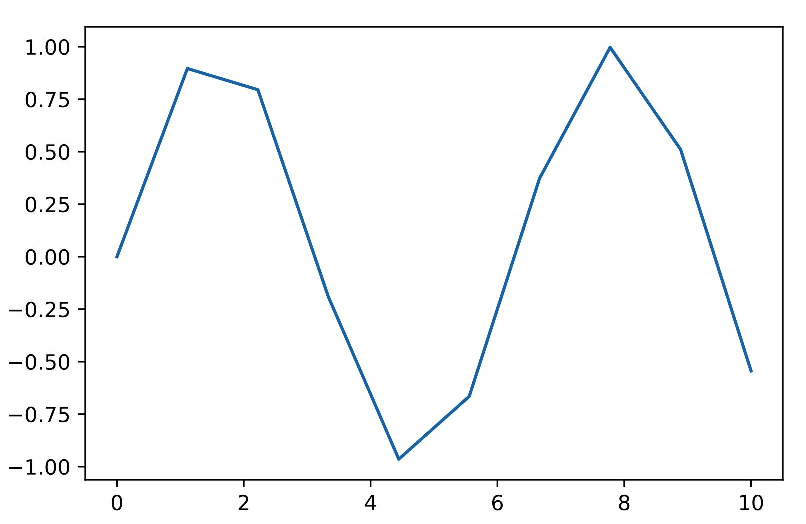
\includegraphics[width=8.5cm]{ch1f1.pdf}
}}    
\end{center}

We end with a slightly more advanced plot, showing how to change line style and markers, and add axis labels and a legend. The NumPy \code{cos} function takes the cosine of the array. The \code{plt.subplots} command makes a new figure and returns handles to the figure \code{fig} and axes \code{ax}. We can then use \code{ax} to plot the functions (\code{plot}), set the axes labels (\code{set\_xlabel} and \code{set\_ylabel}), and add a legend (\code{legend}). The last line saves the figure as a png image. Try also different values of \code{n} to see how the plot changes:

\begin{center}
\begin{lstlisting}[language=Python, frame=single]
n = 25
x = np.linspace(0, 10,n)
y = np.cos(x)
# Make a figure
fig, ax = plt.subplots()
# plot cosine function as a red line
ax.plot(x, y, "r", label="Cosine")
x = np.linspace(0,10,5)
y = 0.01*x**2
# plot quadratic funcion as blue dashed line with dots
ax.plot(x,y,"bo--", label="Quadratic")
# label axes
ax.set_xlabel("Time")
ax.set_ylabel("Amplitude")
# Add legend
ax.legend()
# Save the figure as a png with resolution 300 dpi
fig.savefig("my_first_plot.png", dpi=300);
\end{lstlisting}
\fbox{
\parbox{\textwidth - 2 \fboxsep}{
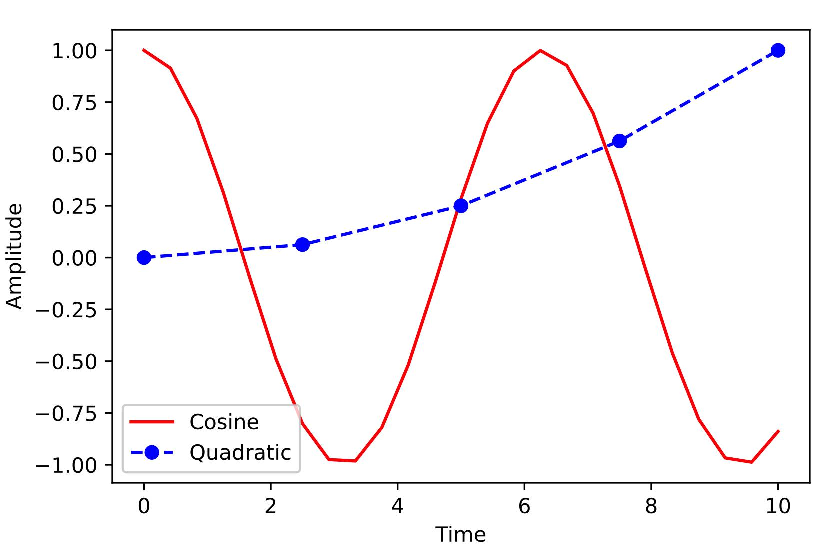
\includegraphics[width=8.5cm]{ch1f2.pdf}
}}   
\end{center}

% SECTION: EXERCISES
\section{Exercises}

\begin{enumerate}
    \item Write a program that prints each number from 1 to 20 on a new line. For each multiple of 3, print "Fizz" instead of the number. For each multiple of 5, print "Buzz" instead of the number. For numbers which are multiples of both 3 and 5, print "FizzBuzz" instead of the number. The correct answer is: 1 2 Fizz 4 Buzz Fizz 7 8 Fizz Buzz 11 Fizz 13 14 FizzBuzz 16 17 Fizz 19 Buzz. \textit{Hint:} You will need to use a loop and conditionals to solve this problem.
    
    \item Use the module \code{mylib.py} to convert the following angles in degrees to radians and vice versa: 0, 45, 90, 135, 180, 225, 270, 315, 360. Print the results in a neatly way.
    
    \item Given two 3 $\times$ 3 matrices \textbf{A} = [ [1, 2, 3], [4, 5, 6], [7, 8, 9] ] and \textbf{B} = [ [5, 7, 2], [3, 5, 1], [2, 4, 3] ], compute: 
    \begin{enumerate}
    \item  the sum of the matrices (\textbf{A} + \textbf{B}), 
    \item  The difference of the matrices (\textbf{A} - \textbf{B}), 
    \item  The product of the matrices (\textbf{AB}), 
    \item  The sum of all elements of matrix \textbf{B}, 
    \item  The column sum of matrix \textbf{A}, 
    \item  The row sum of matrix \textbf{A}, 
    \item  The transpose $(\textbf{A}^T)$ of matrix \textbf{A}, 
    \item  The product $\textbf{AA}^T$. What is this product equal to?
    \end{enumerate} 
    
    \textit{Hint}: Check the functions \code{add}, \code{subtract}, \code{dot}, \code{sum} and \code{transpose} in the NumPy library. 
    
    \item The apparent dip $\alpha$ of a plane is given by the equation:
    
    \begin{equation}
        \tan\alpha=\tan\delta\sin\beta
    \end{equation}
    
    where $\delta$ is the true dip of the plane, and $\beta$ is the orientation of the vertical profile along which the dip is measured (Fig. \ref{fig:strikedip}b). 
    
    \begin {enumerate}
    \item Make a function to compute the apparent dip $\alpha$ from the true dip $\delta$ and the orientation of the profile $\beta$. Angles should be entered in radians.
    \item Use this function to make a graph of profile orientation $\beta$ (0 to 90\degree) versus apparent dip $\alpha$ (0 to 90\degree), for values of true dip $\delta$ of 10, 20, 30, 40, 50, 60, 70, and 80\degree. The graph should look like Figure 1.1 below. \textit{Hint:} You need to use the NumPy and Matplotlib libraries. This problem is hard, don't give up.
    \end{enumerate}
    
    \begin{figure}[ht]
        \centering
        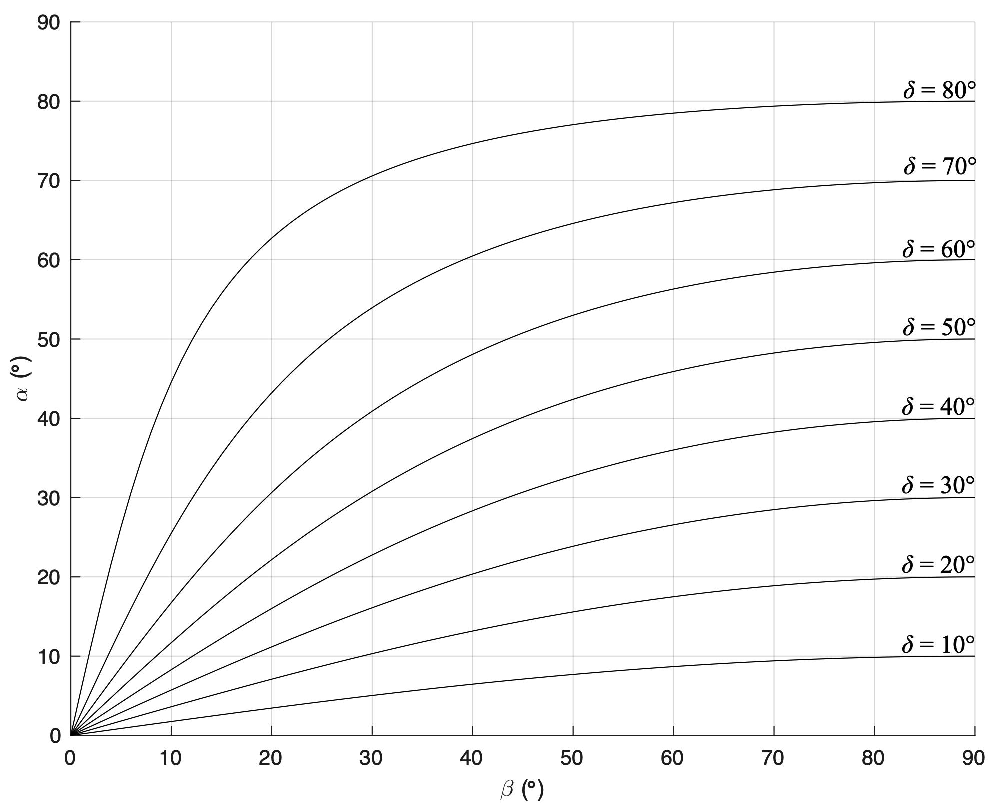
\includegraphics[width=11cm]{ch1f3.pdf}
        \caption{Apparent dip $\alpha$ as function of the profile orientation $\beta$ and true dip $\delta$.}
        \label{fig:apparentdip}
    \end{figure}
\end{enumerate}

\addcontentsline{toc}{section}{References}
\section*{References}

Allmendinger, R.W., Cardozo, N. and Fisher, D.W. 2012. Structural Geology Algorithms: Vectors and Tensors. Cambridge University Press.

Frodeman, R. 1995. Geological reasoning: Geology as an interpretive and historical science. GSA Bulletin 107, 960-968.

Jacobs, C.T., Gorman, G.J., Rees, H.E. and Craig, L.E. 2016. Experiences with efficient methodologies for teaching computer programming to geoscientists. Journal of Geological Education 64, 183-198.

Ragan, D.M. 2009. Structural Geology: An Introduction to Geometrical Techniques. Cambridge University Press.

% CHAPTER 2: UNDERSTANDING LOCATION
\chapter{Understanding location}

% SECTION: LOCATION: HOW DO WE KNOW WHERE WE ARE?
\section{Location}

Understanding where we are located or where an object of interest is located is very important in geosciences. Geographic information science is the study of geographic information; it includes theory and concepts and provides methods to combine and analyze spatial data (Watson, 2017). Geographic information systems is the software and technology that supports the application of geographic information theory (Watson, 2017). GIS is an acronym used for either geographic information systems or geographic information science. 

Geosciences are Earth-based and so location-based. The geographic aspect is highly applicable for the geosciences. The basic usage of GIS is cartographic – making maps. In this chapter, you will become familiar with some of the basic concepts in defining locations on the Earth. These concepts are also used for defining locations on other planets as well.

% SECTION: GEODESY BASICS
\section{Geodesy basics}

Geodesy is “the branch of mathematics dealing with the shape and area of the Earth or large portions of it” (Lexico, 2019); however, the discipline is expanding to include other planets. We need geodesy to model the Earth and make calculations because the Earth is not a perfect sphere nor flat.

\subsection{Scales}

In cartography, we use scales to describe how the real world length has been reduced to fit on a page or screen. Usually, map scales are described as ratios, such as 1:50,000. When we describe the scale, we say it is either small or large. The description of small or large refers to the scale, not the size of the area. Therefore, if we describe a scale as small, it means the fraction described by the scale ratio is small; this in turn means the map covers a large area. The inverse is true for large scales; the fraction described by the scale is large and in turn covers a small area (Kraak and Ormeling, 2003, Lisle et al., 2011). There is not an official categorical differentiation between small and large scales. Generally speaking, small scale maps cover regions, countries, and continents, while large scale maps cover neighborhoods, towns, or counties. The following example illustrates this.

\subsection*{Example 1: Understanding Map Scales}

A map has a scale of 1:1,000,000. Would you refer to this as a small or large scale?

\begin{enumerate}
    \item First, rewrite this as a fraction: 1/1,000,000
    \item Is this a small fraction or a large fraction? This is a relatively small fraction, so it is a small scale. 
\end{enumerate}

Figure 2.1 is an example of a map with a scale of 1:1,000,000.

\begin{figure}[ht]
    \centering
    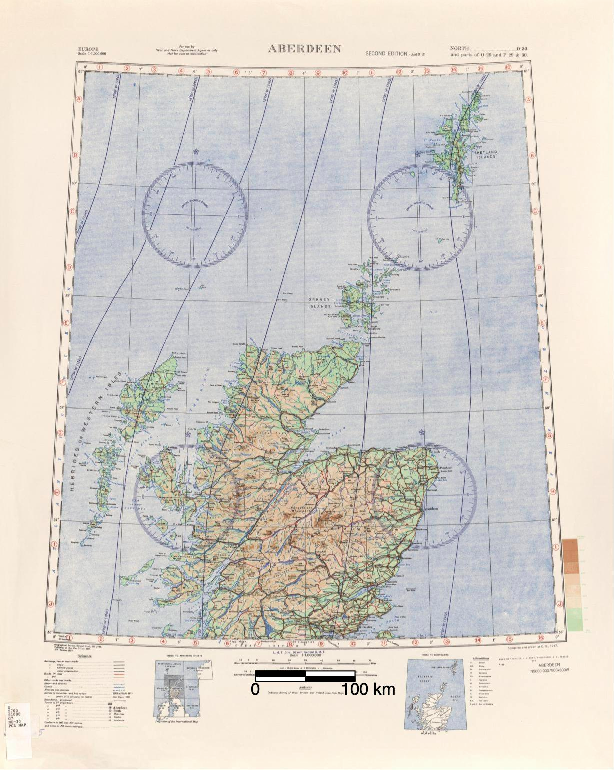
\includegraphics[width=10cm]{ch2f1.pdf}
    \caption{A historical map of northern Scotland at the scale of 1:1,000,000 (Geographic Section - General Staff, 1941).}
\end{figure}

A map has a scale of 1:10,000. Would you refer to this as a small or large scale?

\begin{enumerate}
    \item First, rewrite this as a fraction: 1/10,000
    \item Is this a small fraction or a large fraction? This is a relatively large fraction, so it is a large scale. 
\end{enumerate}

Figure 2.2 is an example of a map with a scale of 1:10,000.

\begin{figure}[ht]
    \centering
    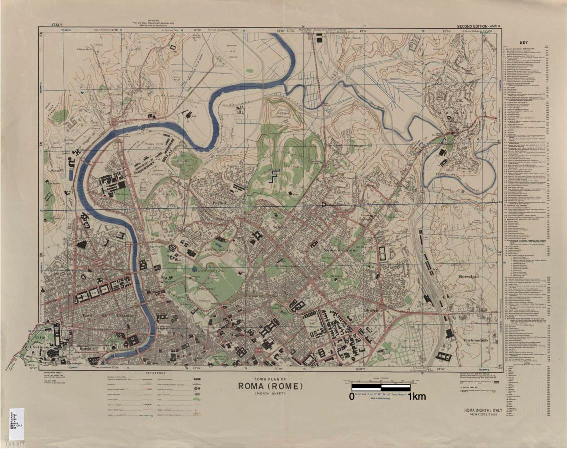
\includegraphics[width=12cm]{ch2f2.pdf}
    \caption{A historical map of Rome, Italy at the scale of 1:10,000 (C.I.U. and War Office, 1944).}
\end{figure}

\subsection{Authalic Sphere}

The authalic sphere is a sphere used for the basic surface for mapping (Fig. 2.3); its surface area is the same as the ellipsoid (Robinson et al., 1995). Based on the WGS-84 ellipsoid, the Earth has an equatorial radius of 6371 km and a circumference of 40,030.2 km. The radius is an often-used constant in geodesy (Robinson et al., 1995). The authalic sphere is used in small scale mapping (small scale covers a large area) because the difference between the authalic sphere and the ellipsoid is minimum over large areas (Robinson et al., 1995).

\begin{figure}[ht]
    \centering
    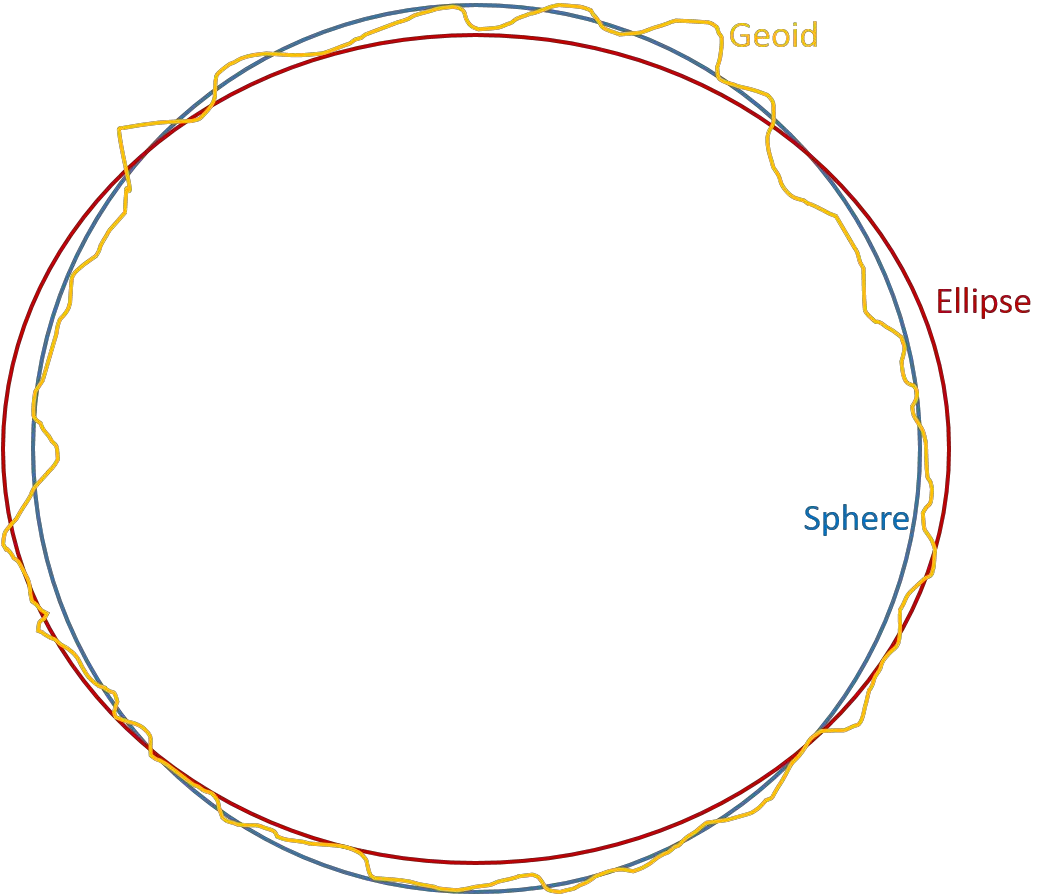
\includegraphics[width=9cm]{ch2f3.pdf}
    \caption{Highly stylized comparison of sphere, ellipse, and geoid.}
\end{figure}

\subsection{Ellipsoidal Earth}

Due to gravity, the Earth flattens at the poles. In a cross-section, the Earth looks like an oblate ellipsoid (Fig. 2.3) (Robinson et al., 1995). Oblateness refers to flatness. When mapping over small areas (large scale mapping), the oblateness of the ellipsoid must be taken into account. The GPS network uses the WGS-84 ellipsoid (Robinson et al., 1995).

There are varying ellipsoidal measurements on different continents and times. These continental differences are due to gravity. Temporal differences are due to technological accuracy. The WGS-84 ellipsoid is based on satellite observations and is accepted as being highly accurate (Robinson et al., 1995).

\subsection{Geoid}

Geoid means Earth-like and is in 3D. It is based on an equipotential gravity surface. The geoid follows the mean sea level in oceans and hypothetical sea-level canals on the continents (Robinson et al., 1995). Due to geology (rock density) and topography, the geoid deviates from the ellipsoid (Fig. 2.3). The geoid is a “reference surface for ground surveyed horizontal and vertical positions” (Robinson et al., 1995).

% SECTION: PROJECTIONS
\section{Projections} \label{projections}

A projection is a mathematical equation to transfer a region, of whatever size, of the round Earth onto a flat surface. Projections are used because distance and surface area calculations are more difficult on a sphere. A flat map can show greater detail than a sphere and is more transportable. Imagine how large a globe you would need to sufficiently show the streets in your neighborhood! We need projections to transform our 3D ellipsoidal Earth onto a flat map. Projections may be based on the authalic sphere, ellipsoid, or geoid.

Before proceeding, take a moment to look over an informational \href{https://pubs.usgs.gov/gip/70047422/report.pdf}{pictographic} by the U.S. Geological Survey describing different types of projection.

\subsection{Distortions}

All projections have distortions that vary by projection type (i.e. transverse Mercator vs. Miller cylindrical – see pictograph mentioned in previous section). Selecting a projection depends on discipline, size of area, orientation of area, regional standards, map purpose, and map scale. There are many resources for determining which projection you should use. Large-scale mapping uses conformal projection because angles measured on the ground are the same as those in the map (Iliffe and Lott, 2008). Four types of distortion are: area, shape, direction, and distance. The Tissot’s Indicatrix is a graphic device to show the distortion at a point (Robinson et al., 1995). We will investigate this phenomenon using the Python library \href{https://scitools.org.uk/cartopy/docs/latest/#}{Cartopy}. To install this library, follow the steps below:

\subsection*{Installing Cartopy}

We will use the Cartopy library to visualize projection distortions using the Tissot’s Indicatrix. We will make a special Cartopy Environment in Anaconda. This is because Cartopy dependencies are lower than some other libraries we’ll be using. This happens from time to time when we use open-source libraries.

\begin{enumerate}
    \item Open Anaconda Navigator.
    \item In the left panel, click on \code{Environments}.
    \item In the middle panel, click \code{Create} to create a new environment
    \item Name this environment: \code{ch2cartopy}
    \item Select Python version 3.8 or later
    \item Click \code{Create}. This will take a few minutes.
    \item We need to install Cartopy. In the right panel in the search field, type: \code{cartopy}
    \item You will get the message \code{0 packages available matching cartopy} since Cartopy is not installed.
    \item In the right panel, change \code{Installed} to \code{Not installed}
    \item Cartopy now shows up\footnote{If it does not, press \code{Update index} in the right panel.}. Click the check box next to \code{cartopy}.
    \item In the screen lower right corner, click \code{Apply}
    \item Please wait while Cartopy is collected and then click \code{Apply}
    \item The Cartopy library and any dependencies will be installed or updated. This may take a few minutes\footnote{If Cartopy is lower than v. 0.21, you will need to downgrade the Matplotlib from 3.6.2 to 3.5.2. Open a terminal or command window. Type \code{conda activate ch2cartopy} followed by \code{Enter}, and then \code{conda install matplotlib==3.5.2} followed by \code{Enter}.}. 
    \item Click on \code{Home}
    \item Click on \code{Install} under Jupyter Notebook.
    \item Click on \code{Launch} under Jupyter Notebook.
   
\end{enumerate}

\subsection*{Example 2: Tissot's Indicatrix}

This example will introduce you to understanding distortions in projections. As you change the projection name, a different mathematical equation will be used to portray the round Earth in a flat presentation. Pay particular attention to the size, shape, and spacing of the ellipses describing the distortion. The Tissot’s Indicatrix quickly and easily visualizes the changes in area and spatial relationships between different projections.

The notebook \href{https://github.com/nfcd/compGeo/blob/master/source/notebooks/ch2-1.ipynb}{ch2-1} contains this example. If you just launched Jupyter Notebook as indicated above, open the notebook. If you closed Anaconda, follow these steps:

\begin{enumerate}
    \item Open Anaconda Navigator
    \item Click on \code{Environments}
    \item Choose \code{ch2cartopy}
    \item Click \code{Home}
    \item Launch Jupyter Notebook
    \item Open the notebook \code{ch2-1}
\end{enumerate}{}

This example starts with the Plate Carree projection (\href{https://scitools.org.uk/cartopy/docs/latest/gallery/tissot.html}{Cartopy, 2018b}). Run the code below:

\begin{center}
\begin{lstlisting}[language=Python, frame=single]
# Import cartopy and matplotlib
import cartopy.crs as ccrs
import matplotlib.pyplot as plt

# Hide warnings
import warnings 
warnings.simplefilter("ignore")

# Figure
fig = plt.figure(figsize=(10, 5))
# Plate Carree projection
ax = plt.axes(projection=ccrs.PlateCarree())

# Make the map global rather than have it zoom in to
# the extents of any plotted data
ax.set_global()

# Earth image
ax.stock_img()
# Coastlines
ax.coastlines()

# Tissot"s indicatrix: Orange ellipses
ax.tissot(facecolor="orange", alpha=0.4);
\end{lstlisting}
\fbox{
\parbox{\textwidth - 2 \fboxsep}{
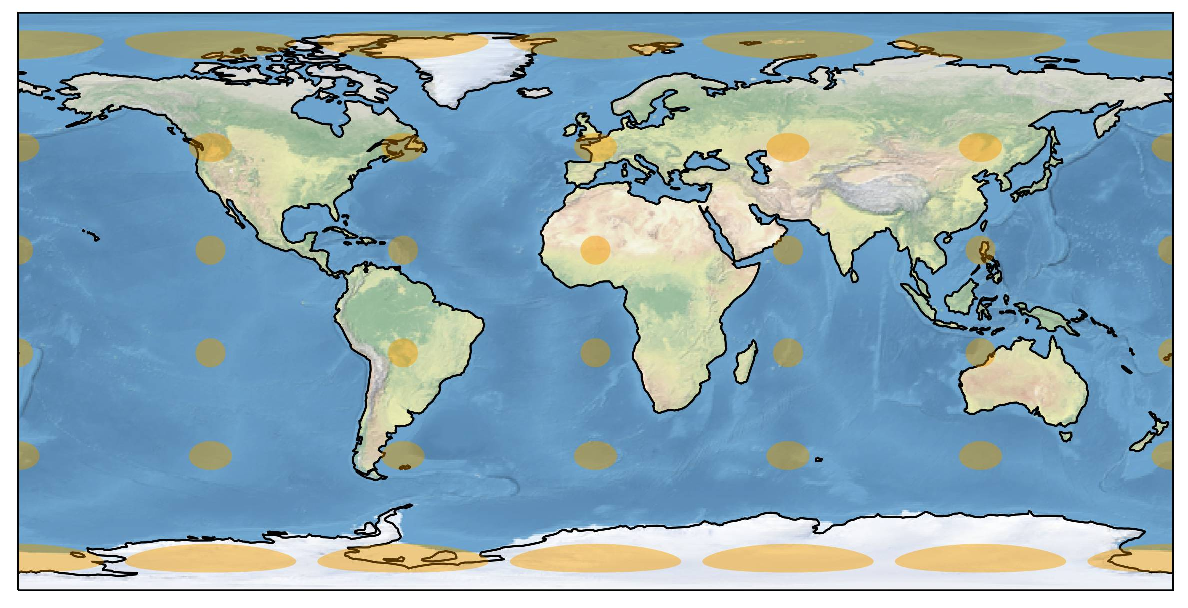
\includegraphics[width=11cm]{ch2f4.pdf}
}}   
\end{center}

The Tissot’s Indicatrix is symbolized by the orange ellipses. Closer to the poles, the ellipses become more oblate; while closer to the Equator, they are more circular. The Plate Carrée projection is a specific form of the Equidistant Cylindrical projection. Plate Carrée has the latitude of origin at the Equator.

Change the code to use the Mollweide projection:

\begin{center}
\begin{lstlisting}[language=Python, frame=single]
# Figure
fig = plt.figure(figsize=(10, 5))
# Mollweide projection
ax = plt.axes(projection=ccrs.Mollweide())

# Make the map global rather than have it zoom in to
# the extents of any plotted data
ax.set_global()

ax.stock_img()
ax.coastlines()

ax.tissot(facecolor="orange", alpha=0.4);
\end{lstlisting}
\fbox{
\parbox{\textwidth - 2 \fboxsep}{
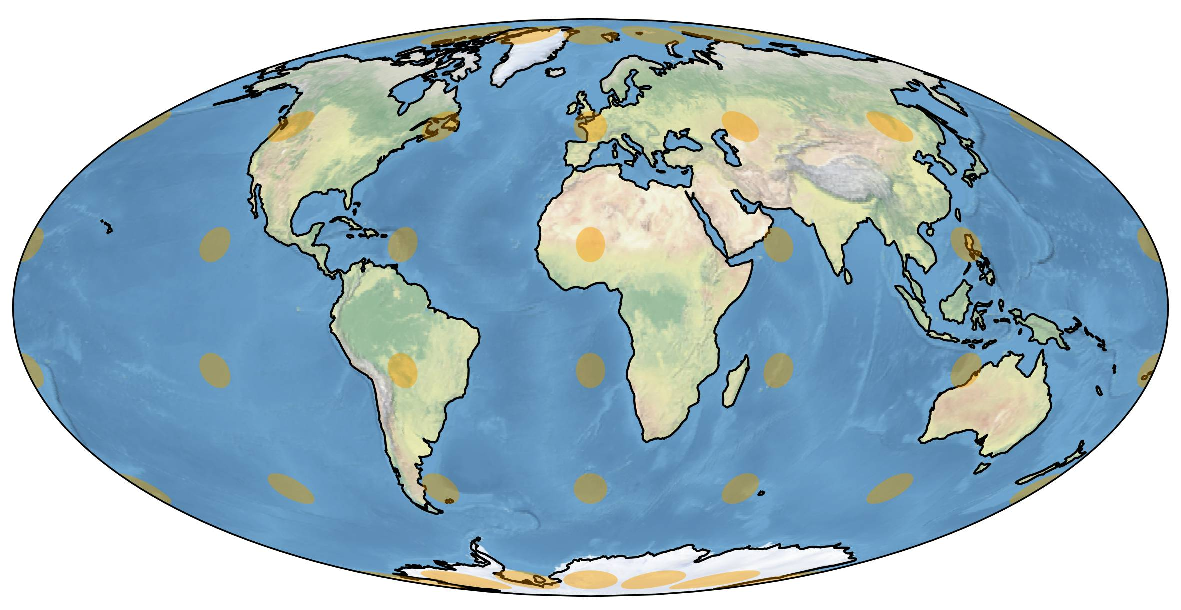
\includegraphics[width=11cm]{ch2f5.pdf}
}}   
\end{center}

Notice how the sizes of the ellipses are very similar throughout the map. All of the ellipses are more rounded and circular regardless of their position, as compared to the Plate Carrée projection. Mollweide is often used for world maps.

Cartopy has a list of projections that are included in the library  (\href{https://scitools.org.uk/cartopy/docs/latest/crs/projections.html}{Cartopy, 2018a}). Change the code above to project the map in Azimuthal Equidistant. 

% SECTION: COORDINATE REFERENCE SYSTEMS AND DATUMS
\section{Reference systems and datums}

A coordinate reference system is a coordinate system that has been referenced to a datum. A datum is the location used for a reference point from which spatial measurements are made. There are geographic and Cartesian coordinate systems. Coordinates are for specific locations on the Earth. They can be expressed as geographic using latitude and longitude. Latitude are parallels that are evenly spaced and longitude are meridians that converge at the poles. These are measured in degrees. Cartesian coordinates are expressed in x and y and may have units that are meters, feet, or kilometers, for example. Coordinates only have meaning when the coordinate system and datum are known (Iliffe and Lott, 2008, Robinson et al., 1995). 

\subsection*{Example 3: Defining the coordinate reference system}

In any GIS program, including spatial libraries and code, the user must ensure that the coordinate reference system is defined for the spatial data. The GIS software will make assumptions, sometimes erroneous, if the coordinate reference system is not properly defined. In this example, we will see a demonstration of these assumptions and how to prevent them. This example is from the SciTools tutorials to understand Cartopy (\href{https://scitools.org.uk/cartopy/docs/latest/tutorials/understanding_transform.html}{Cartopy, 2018c}).

In Cartopy, there are two keywords that you must understand in order to properly display your data. The “projection” argument is used for display of your data. This only affects the map or plot. It does not define the coordinate reference system of the data itself. The “transform” argument, on the other hand, defines the coordinate reference system. The best practice is to define both of these. We will investigate the error that occurs when the best practice is not followed and compare this to when the best practice is followed. The notebook \href{https://github.com/nfcd/compGeo/blob/master/source/notebooks/ch2-2.ipynb}{ch2-2} contains this example.

First we will create some dummy data on a regular latitude/longitude grid\footnote{In Python, the backslash character \code{$\backslash$} can be used to split a long line of code.}:

\begin{center}
\begin{lstlisting}[language=Python, frame=single]
import numpy as np

lon = np.linspace(-80, 80, 25)
lat = np.linspace(30, 70, 25)
lon2d, lat2d = np.meshgrid(lon, lat)

data = np.cos(np.deg2rad(lat2d) * 4) + \
    np.sin(np.deg2rad(lon2d) * 4)
\end{lstlisting}
\end{center}

In order to demonstrate the error before "best practice", we will create a map using the Plate Carree projection but only specify the \code{projection} argument. Remember that the best practice requires both \code{projection} and \code{transform} arguments to be defined.

\begin{center}
\begin{lstlisting}[language=Python, frame=single]
# Import cartopy and matplotlib
import cartopy.crs as ccrs
import matplotlib.pyplot as plt

# Hide warnings
import warnings 
warnings.simplefilter("ignore")

# The projection keyword determines how the plot will look
fig = plt.figure(figsize=(6, 3))
ax = plt.axes(projection=ccrs.PlateCarree())
ax.set_global()
ax.coastlines()

# didn't use transform, but looks ok...
ax.contourf(lon, lat, data);
\end{lstlisting}
\fbox{
\parbox{\textwidth - 2 \fboxsep}{
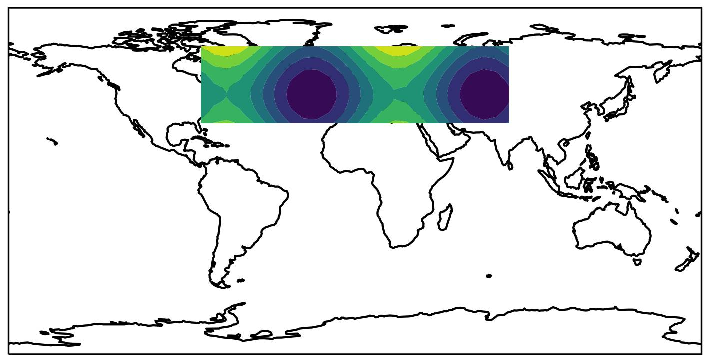
\includegraphics[width=10cm]{ch2f6.pdf}
}}   
\end{center}

In this case, the data just happen to fall in the correct location. Now, we will define the data coordinate reference system (first line of code below) and add the \code{transform} argument to the plot (second last line of code below).

\begin{center}
\begin{lstlisting}[language=Python, frame=single]
# The data are defined in lat/lon coordinate system, 
# so PlateCarree() is the appropriate choice:
data_crs = ccrs.PlateCarree()

# The projection keyword determines how the plot will look
fig = plt.figure(figsize=(6, 3))
ax = plt.axes(projection=ccrs.PlateCarree())
ax.set_global()
ax.coastlines()

# use transform
ax.contourf(lon, lat, data, transform=data_crs);
\end{lstlisting}
\fbox{
\parbox{\textwidth - 2 \fboxsep}{
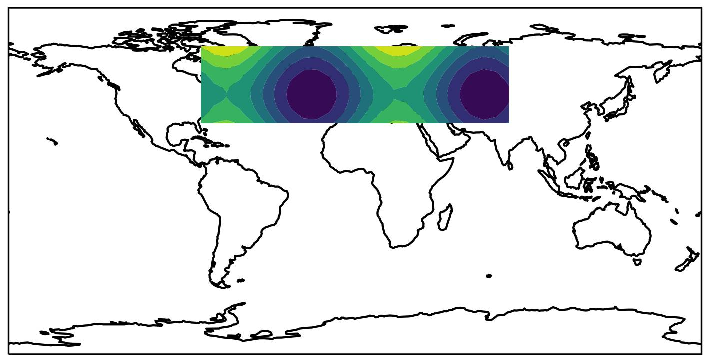
\includegraphics[width=10cm]{ch2f6.pdf}
}}   
\end{center}

You will notice that our plot remains unchanged. The assumption, as stated previously, is that if the coordinate reference system of the data is undefined, it is the same as the map (or plot) projection. In the example above, this has been the case. Let us now investigate what happens when changing the projection of the map without defining the coordinate reference system of the data. We now define the projection to \code{RotatedPole} and omit the \code{transform} argument to see what happens:

\begin{center}
\begin{lstlisting}[language=Python, frame=single]
# Now we plot a rotated pole projection
projection = ccrs.RotatedPole(pole_longitude=-177.5, pole_latitude=37.5)
fig = plt.figure(figsize=(6, 3))
ax = plt.axes(projection=projection)
ax.set_global()
ax.coastlines()

# didn't use transform, uh oh!
ax.contourf(lon, lat, data); 
\end{lstlisting}
\fbox{
\parbox{\textwidth - 2 \fboxsep}{
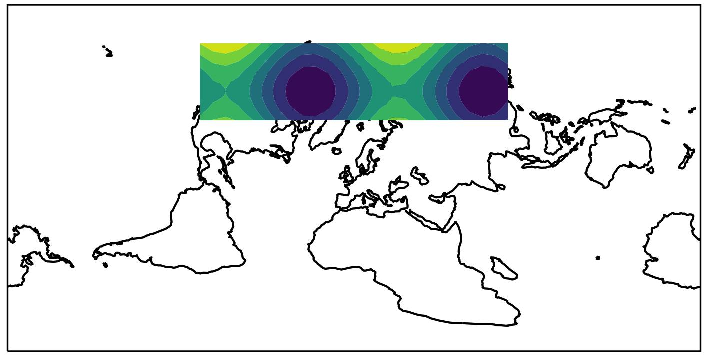
\includegraphics[width=10cm]{ch2f7.pdf}
}}   
\end{center}

In this case, we see that the country boundaries have rotated and changed shape, however, the data did not move with the the country boundaries. We made a wrong assumption in the data definition. Therefore we need to define the \code{transform} argument:

\begin{center}
\begin{lstlisting}[language=Python, frame=single]
# A rotated pole projection again...
projection = ccrs.RotatedPole(pole_longitude=-177.5, pole_latitude=37.5)
fig = plt.figure(figsize=(6, 3))
ax = plt.axes(projection=projection)
ax.set_global()
ax.coastlines()

# ...but now using the transform argument
ax.contourf(lon, lat, data, transform=data_crs);
\end{lstlisting}
\fbox{
\parbox{\textwidth - 2 \fboxsep}{
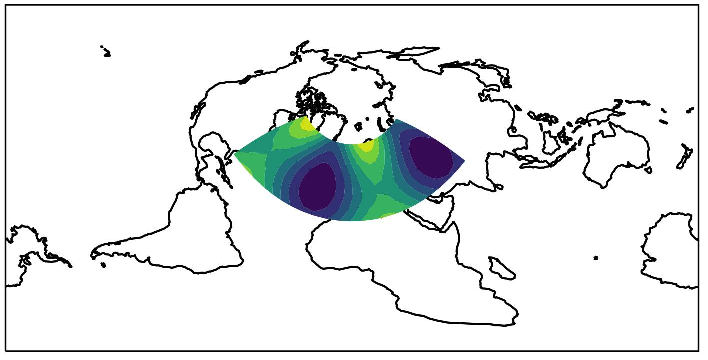
\includegraphics[width=10cm]{ch2f8.pdf}
}}   
\end{center}

Now the data are correctly projected. Get in the habit of always defining the coordinate reference system and the map plot projection. It will save headaches and misunderstandings of the data.

Here is another script using an entirely different projection and additional plotting parameters. Can you figure out what the script will produce before running the cell? Notice the presence of the Matplotlib function \code{subplot}. What do you think this function does?

\begin{center}
\begin{lstlisting}[language=Python, frame=single]
# We can choose any projection we like...
projection = ccrs.InterruptedGoodeHomolosine()
fig = plt.figure(figsize=(6, 7))
ax1 = plt.subplot(211, projection=projection)
ax1.set_global()
ax1.coastlines()
ax2 = plt.subplot(212, projection=ccrs.NorthPolarStereo())
ax2.set_extent([-180, 180, 20, 90], crs=ccrs.PlateCarree())
ax2.coastlines()

# ...as long as we provide the correct transform, 
# the plot will be correct
ax1.contourf(lon, lat, data, transform=data_crs)
ax2.contourf(lon, lat, data, transform=data_crs);
\end{lstlisting}
\end{center}

Now that you have worked through the exercise, you should have an understanding of why it is important to fully define the coordinate reference system and the projection when creating a map.

% SECTION: COORDINATE CONVERSION AND TRANSFORMATION
\section{Conversion vs. transformation}

When working with data collected from several sources or in different coordinate reference systems, the data must be redefined to have the same coordinate reference system and datum. Consistent coordinate reference systems for data in a map is important because there may be spatial differences between the coordinate reference systems creating locational errors. A coordinate conversion is when the coordinate reference systems have the same datum. A coordinate transformation is when the coordinate reference systems have different datums.

When making a map, all of the data in the map should have the same coordinate reference system definition. Software include many definitions and transformations but refer to Snyder (1987) and International Association of Oil and Gas Producers (2018) for projection formulae (Iliffe and Lott, 2008). In Example 2, the Tissot’s Indicatrix ellipses did not change coordinate reference systems. The method used to plot the ellipses changed. In Example 3, we also only changed the projection of the map, not the coordinate reference system. In the following examples, we will make coordinate conversions and transformations. For this purpose, we will use the \href{https://pypi.org/project/pyproj/}{pyproj} Python library and examples from the pyproj documentation (\href{https://pyproj4.github.io/pyproj/stable/api/transformer.html?highlight=transformer}{Whitaker, 2019}).

\subsection*{Installing pyproj}

A version of pyproj was installed with Cartopy, but you need the latest version which has different dependencies than Cartopy. You will create a new environment.

\begin{enumerate}
    \item Open Anaconda Navigator.
    \item In the left panel, click on \code{Environments}
    \item In the middle panel, click \code{Create} to create a new environment
    \item Name this environment: \code{ch2pyproj}
    \item Select Python version 3.8 or later
    \item Click \code{Create}. This will take a few minutes
    \item We need to install pyproj. In the right panel in the search field, type: \code{pyproj}
    \item You will get the message \code{0 packages available matching pyproj} since pyproj is not installed. 
    \item In the right panel, change \code{Installed} to \code{Not installed}
    \item pyproj now shows up. Click the check box next to \code{pyproj}.
    \item In the screen lower right corner, click \code{Apply}
    \item Please wait while pyproj is collected and then click \code{Apply}
    \item The pyproj library and any dependencies will be installed or updated. This may take a few minutes.
    \item Click on \code{Home}
    \item Click on \code{Install} under Jupyter Notebook.
    \item Click on \code{Launch} under Jupyter Notebook.
\end{enumerate}

\subsection*{Example 4: Coordinate conversion}

The notebook \href{https://github.com/nfcd/compGeo/blob/master/source/notebooks/ch2-3.ipynb}{ch2-3} contains this example. If you just launched Jupyter Notebook as indicated above, open the notebook. If you closed Anaconda, follow these steps:

\begin{enumerate}
    \item Open Anaconda Navigator
    \item Click on \code{Environments}
    \item Choose \code{ch2pyproj}
    \item Click \code{Home}
    \item Launch Jupyter Notebook
    \item Open the notebook \code{ch2-3}
\end{enumerate}{}

We have a coordinate pair defined in decimal degrees of latitude and longitude. The longitude is -120.108\degree\space and latitude is 34.36116666\degree. We want to make a coordinate conversion from latitude and longitude to Universal Transverse Mercator, where the point is defined by east and north coordinates in meters. To learn more about Universal Transverse Mercator (UTM), refer to (Snyder, 1987). In the code, we use the pyproj \code{Proj} function. We can only use \code{Proj} when making a coordinate conversion (i.e. the same datum):

\begin{center}
\begin{lstlisting}[language=Python, frame=single]
# Import pyproj
from pyproj import Proj

# Construct the projection matrix
p = Proj(proj="utm",zone=10,ellps="WGS84", 
         preserve_units=False)

# Apply the projection to the lat-long point
x,y = p(-120.108, 34.36116666)

print(f"x={x:9.3f}, y={y:11.3f}")
\end{lstlisting}
\fbox{
\parbox{\textwidth - 2 \fboxsep}{
x=765975.641, y=3805993.134
}}   
\end{center}

This is the same location but only expressed in east and north coordinates in meters using the UTM coordinate reference system. The datum used is WGS84. We can convert the UTM coordinates back to latitute and longitude by adding two lines of code:

\begin{center}
\begin{lstlisting}[language=Python, frame=single]
# Apply the inverse of the projection matrix
# to the point in UTM
lon,lat = p(x,y,inverse=True)
print(f"lon={lon:8.8f}, lat={lat:5.8f}")
\end{lstlisting}
\fbox{
\parbox{\textwidth - 2 \fboxsep}{
lon=-120.10800000, lat=34.36116666
}}   
\end{center}

We can confirm that the inverse conversion arrives at the original pair. Let's now try converting several points of different latitude and longitude using a collection of objects in Python, or tuples. Add the following code:

\begin{center}
\begin{lstlisting}[language=Python, frame=single]
# three points in lat-long
lons = (-119.72,-118.40,-122.38)
lats = (36.77, 33.93, 37.62 )
# Apply the projection to the points
x1,y1 = p(lons, lats)
print(x1,y1)
\end{lstlisting}
\fbox{
\parbox{\textwidth - 2 \fboxsep}{
(792763.8631257227, 925321.5373562573, 554714.3009414743)\\ 
(4074377.6167697194, 3763936.9410883673, 4163835.3033114495)
}}   
\end{center}

Now, let's do a more advanced exercise: In the cartographic community, an easy way to communicate the coordinate reference system is to use the EPSG Geodetic Parameter Data set. Every coordinate reference system is given a code. This ensures that if someone uses UTM zone 10 North with datum WGS-84 and tells you UTM zone 10, that you do not accidentally use UTM zone 10 North with datum GRS80, for example.

Earlier in this exercise, we defined the UTM zone in the \code{Proj} function. Here, we will refer to the EPSG code. First, we will take a coordinate pair in longitude and latitude with datum WGS84 and convert it to EPSG:32667. Before proceeding, conduct a quick internet search on what EPSG:32667 means. This is important to understand what we will do next. The first part of the code is:

\begin{center}
\begin{lstlisting}[language=Python, frame=single]
# silence warnings
import warnings 
warnings.simplefilter("ignore")

# initial coordinate conversion
p = Proj(init="EPSG:32667", preserve_units=True, 
         always_xy=True)
# Apply the conversion to the lat-long point
x,y = p(-114.057222, 51.045)
print(f"x={x:9.3f}, y={y:11.3f} (feet)")
\end{lstlisting}
\fbox{
\parbox{\textwidth - 2 \fboxsep}{
x=-5851386.754, y=20320914.191 (feet)
}}   
\end{center}

Let’s dissect this as the pyproj code looks quite a bit different. The first part of the function \code{Proj} calls EPSG:32667. If you looked up EPSG:32667 online, you found that it is for UTM zone 17 North, but the units are in feet. The default mode for \code{Proj} is \code{preserve\_units=False}, which forces any unit to meters. However, we want to see the units in US Survey Feet as the projection defines; therefore, we change the argument to \code{True}.

Now, suppose we want to see the output in meters. How will you amend the code? Here is what you should add:

\begin{center}
\begin{lstlisting}[language=Python, frame=single]
# Print the coordinate pair in meters
p1 = Proj(init="EPSG:32667", preserve_units=False)
x1,y1 = p1(-114.057222, 51.045)
print(f"x={x1:9.3f}, y={y1:11.3f} (meters)")
\end{lstlisting}
\fbox{
\parbox{\textwidth - 2 \fboxsep}{
x=-1783506.250, y=6193827.033 (meters)
}}   
\end{center}

As discussed, you should change \code{preserve\_units=False} and change the unit to be printed from \code{feet} to \code{meters}. Congratulations! You now have a good understanding of coordinate conversions.

\subsection*{Example 5: Coordinate transformation}

We learned earlier that we have a coordinate conversion where a coordinate pair is converted between coordinate reference systems with the same datum. In many instances, the coordinate reference system will also undergo a datum shift – this is a coordinate transformation.

This example is included in the notebook \href{https://github.com/nfcd/compGeo/blob/master/source/notebooks/ch2-4.ipynb}{ch2-4}. We will use the pyproj \code{CRS} and \code{transform} functions. The \code{CRS} function defines the coordinate reference system while the \code{transform} function specifies which coordinate reference system is the original and which is the output. \code{CRS} has the same ability to refer directly to an EPSG code.

The input coordinates are in EPSG:4326, which is a commonly used code. It is the geographic coordinate system with datum WGS84. The output coordinates are EPSG:31984, which is for UTM zone 24 S with datum SIRGAS2000.

\begin{center}
\begin{lstlisting}[language=Python, frame=single]
# Import transform and CRS functions
from pyproj import transform
from pyproj import CRS

# Function transform is deprecated
# Silence warnings
import warnings 
warnings.simplefilter("ignore")

# input coordinates
c1 = CRS("EPSG:4326")
# coordinate pair
y1=-10.754283
x1=-39.866132
# output coordinates
c2 = CRS("EPSG:31984")
# Coordinate transformation
x2, y2 = transform(c1, c2, x1, y1)
print(f"x={x2:9.3f}, y={y2:11.3f}")
\end{lstlisting}
\fbox{
\parbox{\textwidth - 2 \fboxsep}{
x=2930179.850, y=5185231.716
}}   
\end{center}

\subsection*{Example 6: Transforming several points at once}

We have focused our examples on one coordinate pair at a time. The reality is that you will more often have several coordinates to transform at one time. The notebook \href{https://github.com/nfcd/compGeo/blob/master/source/notebooks/ch2-5.ipynb}{ch2-5} explains how to do this.

We have a csv file with two columns: longitude and latitude. Each coordinate pair is the center of a volcano around the world. There are 1,509 volcanoes in our dataset. The original coordinate reference system is geographic coordinates with datum WGS84. We want to make a coordinate transformation of these data points to World Mercator. It will take much too long to manually transform these coordinates as we have done in the notebooks before. Therefore, our new code will read the csv file and create a new csv file\footnote{Notice that the code can be further simplified by the use of the Numpy library or the Pandas library}.

Check that the input (\code{src\_dir}) and output (\code{dst\_dir}) directories match the directory where the csv file is. In this example, the volcanoes file \newline (\href{https://github.com/nfcd/compGeo/blob/master/source/data/ch2-5/volc_longlat.csv}{volc\_longlat.csv}) is in the directory \code{data/ch2-5}. Run the code, you will know the process is finished when the message \code{process completed} and the time of execution are returned:

\begin{center}
\begin{lstlisting}[language=Python, frame=single]
# Thanks to Rustam Zaitov for implementing 
# this new version of the code

# Import libraries
import csv, time
from os import path
from pyproj import Transformer, CRS

src_file = "volc_longlat.csv" # input file
dst_file = "volc_projected.csv" # output file

src_dir = path.abspath("../data/ch2-5") # input directory
dst_dir = path.abspath("../data/ch2-5") # output directory

src_path = path.join(src_dir, src_file)
dst_path = path.join(dst_dir, dst_file)

src_crs = CRS("EPSG:4326") #WGS84
dst_crs = CRS("EPSG:3395") #World Mercator

# create coordinate transformer
# always_xy=True makes projector.transform() accept 
# lon, lat (GIS order) instead of lat, lon
projector = Transformer.from_crs(src_crs, dst_crs, 
                                 always_xy=True)

# source csv file has lon, lat columns
src_header = ["LONGITUDE", "LATITUDE"]

# destinatin csv file will have x, y columns
dst_header = ["x", "y"]

# start benchmark timer
start_time = time.time()

# open destination file in write mode
with open(dst_path, "w") as w:
    # open source file in read mode
    with open(src_path, "r") as r:
        reader = csv.reader(r, dialect="excel")
        # read and skip first header row 
        input_headers = next(reader)         

        writer = csv.writer(w, delimiter=",", quotechar='"',
                            quoting=csv.QUOTE_MINIMAL)
        # Write the output header
        writer.writerow(dst_header)   
        for row in reader:
            try:
                # convert string values inside row 
                # into float values
                lon, lat = [float(val) for val in row]
                x, y = projector.transform(lon, lat)
                writer.writerow([ x, y ])
            except Exception as e:
                # If coordinates are out of bounds, 
                # skip row and print the error
                print (e)

# stop benchmarking
end_time = time.time()

print("process completed in {} seconds"
      .format(end_time-start_time))
\end{lstlisting}
\fbox{
\parbox{\textwidth - 2 \fboxsep}{
process completed in 0.012643098831176758 seconds
}}   
\end{center}

It takes less than one second to run this code! Check the newly created csv file and notice that you now have a listing of coordinates in meters. The EPSG definition of the output coordinate reference system is listed under \code{dst\_crs}. You can easily change this variable to another EPSG and rerun the script. If you wish to run the script on another file, change the \code{src\_file} and \code{dst\_file}, and the \code{src\_dir} and \code{dst\_dir} if the file is in another directory. 

% SECTION: EXERCISES
\section{Exercises}

\begin{enumerate}
    \item So far, you have worked with data sets that have been provided to you. It is an important skill to be able to find data sets online and to prepare them for use in your work. 
    
    The United States Geological Survey (USGS) Earthquake Hazards Program monitors, records, and maintains a global database of earthquake activity. The public can query the archive and download earthquake epicenter data. Go to the \href{https://earthquake.usgs.gov/earthquakes/search/}{Search Earthquake Catalog} page of the USGS. Using the Basic Options, download all of the magnitude 4.5+ earthquakes in the last year in the world. In the Output Options, choose a CSV format.
    
    \begin{enumerate}
        \item Modify the notebook \href{https://github.com/nfcd/compGeo/blob/master/source/notebooks/ch2-5.ipynb}{ch2-5} to transform the earthquake epicenters from latitude-longitude to World Mercator (or another map projection of your choice). Use this \href{https://pubs.usgs.gov/gip/70047422/report.pdf}{pictographic} for further information. The datum of the earthquake epicenters is likely WGS84.
        \item Plot the earthquake epicenters. Make sure to include the outline of the continents. \textit{Hint}: Look at the notebook \href{https://github.com/nfcd/compGeo/blob/master/source/notebooks/ch2-2.ipynb}{ch2-2} for a starting point, and check the \href{https://scitools.org.uk/cartopy/docs/latest/#}{Cartopy} website for examples of how to plot localities on a map.
        \item Now modify your plot to color the earthquakes by depth (red are shallow and blue are deep earthquakes), and the size of the points by the earthquake magnitude. 
        \item Add the volcanoes from Example 6 (\href{https://github.com/nfcd/compGeo/blob/master/source/data/ch2-5/volc_longlat.csv}{volc\_longlat.csv}) to the map (use triangles to indicate volcanoes). Do you see any correlation between the earthquake epicenters and the volcanoes?
        
    \end{enumerate}
\end{enumerate}

\addcontentsline{toc}{section}{References}
\section*{References}

C.I.U. AND WAR OFFICE. 1944. Town Plan of Roma (Rome) (North Sheet), 1:10,000. Washington, D. C.: War Office.

Cartopy. 2018a. Projections [\href{https://scitools.org.uk/cartopy/docs/latest/crs/projections.html}{Online}]. UK: SciTools. [Accessed 19 November, 2019]

Cartopy. 2018b. Tissot’s Indicatrix [\href{https://scitools.org.uk/cartopy/docs/latest/gallery/tissot.html}{Online}]. UK: SciTools. [Accessed 19 November, 2019].

Cartopy. 2018c. Understanding the Transform and Projection Keywords [\href{https://scitools.org.uk/cartopy/docs/latest/tutorials/understanding_transform.html}{Online}]. UK: SciTools. [Accessed 19 November, 2019].

Geographic Section - General Staff. 1941. Aberdeen, 1:1,000,000. Great Britain: War Office.

Iliffe, J. and Lott, R. 2008. Datums and Map Projections: For Remote Sensing, GIS, and Surveying, Dunbeath, Scotland, Whittles.

International Association of Oil and Gas Producers. 2018. Geomatics Guidance Note 7, Part 2 Coordinate conversions and Transformations including Formulas.

Kraak, M.J. and Ormeling, F.J. 2003. Cartography: visualization of geospatial data. Addison Wesley.

Lexico. 2019. Geodesy [\href{https://www.lexico.com/en/definition/geodesy}{Online}]. Oxford. [Accessed August, 2019].

Lisle, R. J., Brabham, P. and Barnes, J. W. 2011. Basic Geological Mapping, Chicester, UK, Wiley-Blackwell.

Robinson, A. H., Morrison, J. L., Muehrcke, P. C., Kimerling, A. J. and Guptill, S. C. 1995. Elements of Cartography, New York, Wiley.

Snyder, J. P. 1987. Map Projections: a working manual. Geological Survey Professional Paper. Washington, D. C., U.S.A.: United States Government Printing Office.

Watson, L. 2017. Spatial-based assessment at continental to global scale: case studies in petroleum exploration and ecosystem services. PhD, Utrecht University.

Whitaker, J. 2019. pyproj Transformer Documentation [\href{https://pyproj4.github.io/pyproj/stable/api/transformer.html?highlight=transformer}{Online}].  [Accessed 7 January, 2020].

% CHAPTER 3: GEOLOGICAL FEATURES
\chapter{Geological features}

% SECTION: PRIMITIVE OBJECTS: LINES AND PLANES
\section{Primitive objects: Lines and planes}

The fundamental geometric features of geology are lines (e.g. a lineation, a fold axis) and planes (e.g. bedding, a foliation). A \textit{line} is the element generated by a moving point. It can be straight or curved. We will treat straight lines here. A \textit{plane} is a flat surface; a line joining two points on the plane lies wholly on its surface, and two intersecting lines on the plane define the plane. This is equivalent to say that three non-collinear points on the plane define the plane (this is the basis for the well-known three-points problem). Obviously, linear features can be curved (e.g. the intersection of bedding with irregular topography), and surfaces can be non-planar (e.g. bedding in a fold). However, even these more complex cases can be expressed as a collection of lines and planes.

% SECTION: MEASURING LINES AND PLANES
\section{Lines and planes orientations}

Two important properties of lines and planes are location (chapter 2) and orientation (this chapter). Lines and planes orientations are measured with respect to the geographic north and the angle downward or upward from the horizontal. We refer to this coordinate system as the spherical coordinate system, and the measurements defining the lines and planes orientations as the spherical coordinates.

% SUBSECTION: PLANES: STRIKE AND DIP
\subsection{Planes: Strike and dip}

A plane orientation can be defined by the angle a horizontal line on the plane makes with the geographic north, known as the \textit{strike}, and the maximum angle measured downward from the horizontal to the plane, known as the \textit{dip} (Fig 3.1a). The strike is measured as an azimuth, an angle between 0 and  360\degree\space (0 = north, 90 = east, 180 = south, 270 = west). The dip is an angle between 0 (horizontal plane) and 90\degree\space (vertical plane). The projection of the dip onto the horizontal is known as the \textit{dip direction} and is always 90\degree\space from the strike. However, is the dip direction plus or minus 90\degree\space the given strike? Which end of the strike line should we use? To avoid ambiguities, we will use a format known as the \textit{right hand rule} (RHR). In the RHR format, one gives the strike such that the dip direction is always the strike plus 90\degree, i.e. the dip direction is to the right of the strike (Fig. 3.1a).

\begin{figure}[ht]
    \centering
    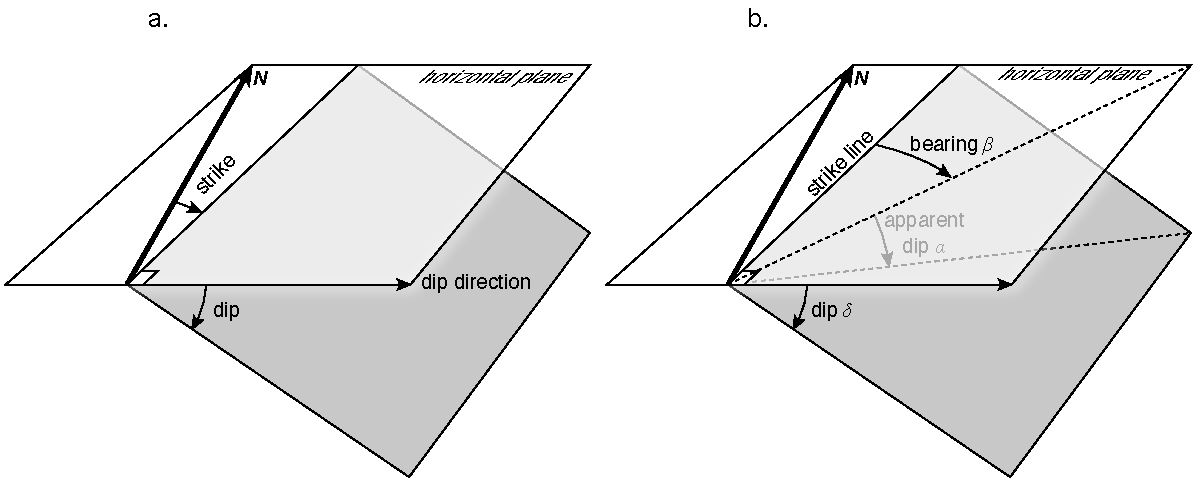
\includegraphics[width=13cm]{ch3f1.pdf}
    \caption{\textbf{a.} Strike and dip of a plane, \textbf{b.} Apparent dip of a plane. Modified from Allmendinger et al. (2012).}
    \label{fig:strikedip}
\end{figure}

It is only along the dip direction that the true dip can be measured, any other direction will give a lower apparent dip (Fig. 3.1b). The relation between the dip ($\delta$) and the apparent dip ($\alpha$) is given by the equation:

\begin{equation}
    \tan\alpha=\tan\delta\sin\beta
\end{equation}

where $\beta$ is the angle between the strike (horizontal) line on the plane and the vertical section on which the apparent dip is measured (Fig. 3.1b). This is also Eq. 1.3, which we plotted in problem 4 of chapter 1 (Fig. \ref{fig:apparentdip}). You can verify that it works by setting $\beta$ = 0 (a cross section parallel to strike) which gives $\alpha$ = 0 (since $\sin(0)$ is 0), and $\beta$ = 90\degree\space ( a cross section perpendicular to strike) which gives $\alpha$ = $\delta$ (since $\sin (90)$ is 1). This leads to an important observation: \textit{A dipping plane shows horizontal in a cross section parallel to strike, and the true dip of the plane can only be observed in a cross section perpendicular to strike}. This is why we should always visualize planes (bedding, faults, etc.) in cross sections perpendicular to strike.

% SUBSECTION: LINES: TREND AND PLUNGE
\subsection{Lines: Trend and plunge or rake}

The orientation of a line is specified by the azimuth of the horizontal projection of the line, or \textit{trend}, and the vertical angle measured downward from the horizontal to the line, or \textit{plunge} (Fig. 3.2a). The plunge has a range between -90 and 90\degree. Positive plunge indicates lines pointing downwards, and negative plunge lines pointing upwards. To measure the trend and plunge one must determine the vertical plane containing the line. This is quite difficult and often results in errors (section 3.2.5). For this reason, and if the line is on a plane, it is more accurate (and convenient) to measure the angle on the plane between the strike line and the line. This angle is known as the rake or pitch (Fig. 3.2b). To avoid any confusion, the rake should be always measured from the given strike and thus it varies between 0 and 180\degree.

\begin{figure}[ht]
    \centering
    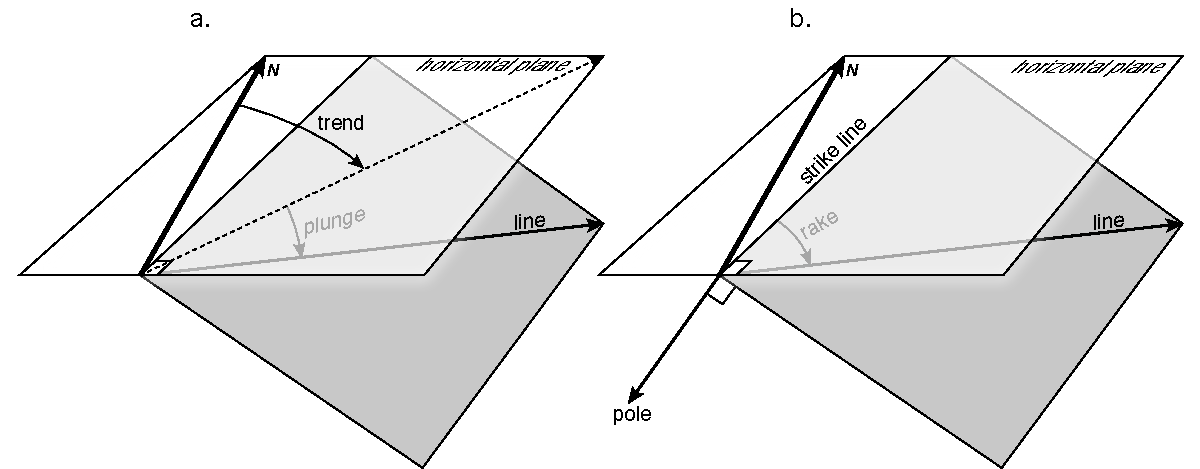
\includegraphics[width=13cm]{ch3f2.pdf}
    \caption{\textbf{a.} Trend and plunge of a line, \textbf{b}. Rake of a line and pole to a plane. Modified from Allmendinger et al. (2012).}
\end{figure}

% SUBSECTION: THE POLE TO THE PLANE
\subsection{The pole to the plane}

Any plane can be uniquely represented by its downward normal. This line is known as the pole to the plane (Fig. 3.2b). If we use the RHR format, the orientation of the pole is given by:

\begin{equation}\label{eq3.2}
    \begin{gathered}
        \text{trend\,of\,pole} = \text{strike\,of\,plane} -90\degree \\
        \text{plunge\,of\,pole} = 90\degree - \text{dip\,of\,plane}
    \end{gathered}
\end{equation}

The pole facilitates analyzing planes graphically and by computation. The module  \href{https://github.com/nfcd/compGeo/blob/master/source/functions/pole.py}{pole} contains two functions to compute the pole from a plane\newline (\code{pole\_from\_plane}), or the plane from its pole (\code{plane\_from\_pole}). These two functions use the function \href{https://github.com/nfcd/compGeo/blob/master/source/functions/zero_twopi.py}{zero\_twopi} which makes sure azimuths are always between 0 and 360\degree. Notice that angles should be entered in radians, and the plane must follow the RHR format.

\begin{center}
\begin{lstlisting}[language=Python, frame=single]
import math
from zero_twopi import zero_twopi

def pole_from_plane(strike,dip):
	'''
	pole_from_plane returns the trend (trd) and 
	plunge (plg) of a pole, given the strike and 
	dip of the plane
	
	NOTE: Input/Output angles are in radians.
	Input strike and dip is in RHR format
	'''
	# Some constants
	east = math.pi/2
	
	# Pole from plane
	trd = zero_twopi (strike - east)
	plg = east - dip
	
	return trd, plg

def plane_from_pole(trd,plg):
	'''
	plane_from_pole returns the strike and dip
	of a plane, given the trend (trd) and 
	plunge (plg) of its pole
	
	NOTE: Input/Output angles are in radians.
	Output strike and dip is in RHR format
	'''
	# Some constants
	pi = math.pi
	east = pi/2
	
	# Unusual case of pole pointing upwards
	if plg < 0.0:
		trd += pi
		plg *= -1.0
		
	# Calculate plane given its pole
	strike = zero_twopi(trd + east)
	dip = east - plg
		
	return strike, dip
\end{lstlisting}
\end{center}

\begin{center}
\begin{lstlisting}[language=Python, frame=single]
import math

def zero_twopi(a):
	"""
	This function makes sure input azimuth (a)
	is within 0 and 2*pi
	
	NOTE: Azimuth a is input/output in radians
	
	Python function translated from the Matlab function
	ZeroTwoPi in Allmendinger et al. (2012)
	"""
	twopi = 2*math.pi
	if a < 0:
		a += twopi
	elif a >= twopi:
		a -= twopi
	
	return a
\end{lstlisting}    
\end{center}

% SUBSECTION: INSTRUMENTS USED IN THE FIELD
\subsection{Instruments used in the field}

Traditionally, geologists use a geological compass/clinometer to measure the orientation of planes and lines in the field. Figure 3.3 shows four of the most common compasses used in geology: the Silva compass (Fig. 3.3a), the Brunton compass (Fig. 3.3b), the Krantz compass (Fig. 3.3c, a less expensive variant of the Freiberg compass), and the Brunton Geo compass (Fig. 3.3d). All these compasses have a magnetic needle that points  to the magnetic north (N or white end of the needle), a horizontal level, and a clinometer (an instrument to measure vertical angles). The Silva compass has an azimuth scale that can be rotated to follow the magnetic needle, while in the other three compasses the azimuth scale is fixed. This is why east-west (E-W) are in the right place in the Silva compass, while they are flipped in the other three compasses (Fig. 3.3a-d).

\begin{figure}[ht]
    \centering
    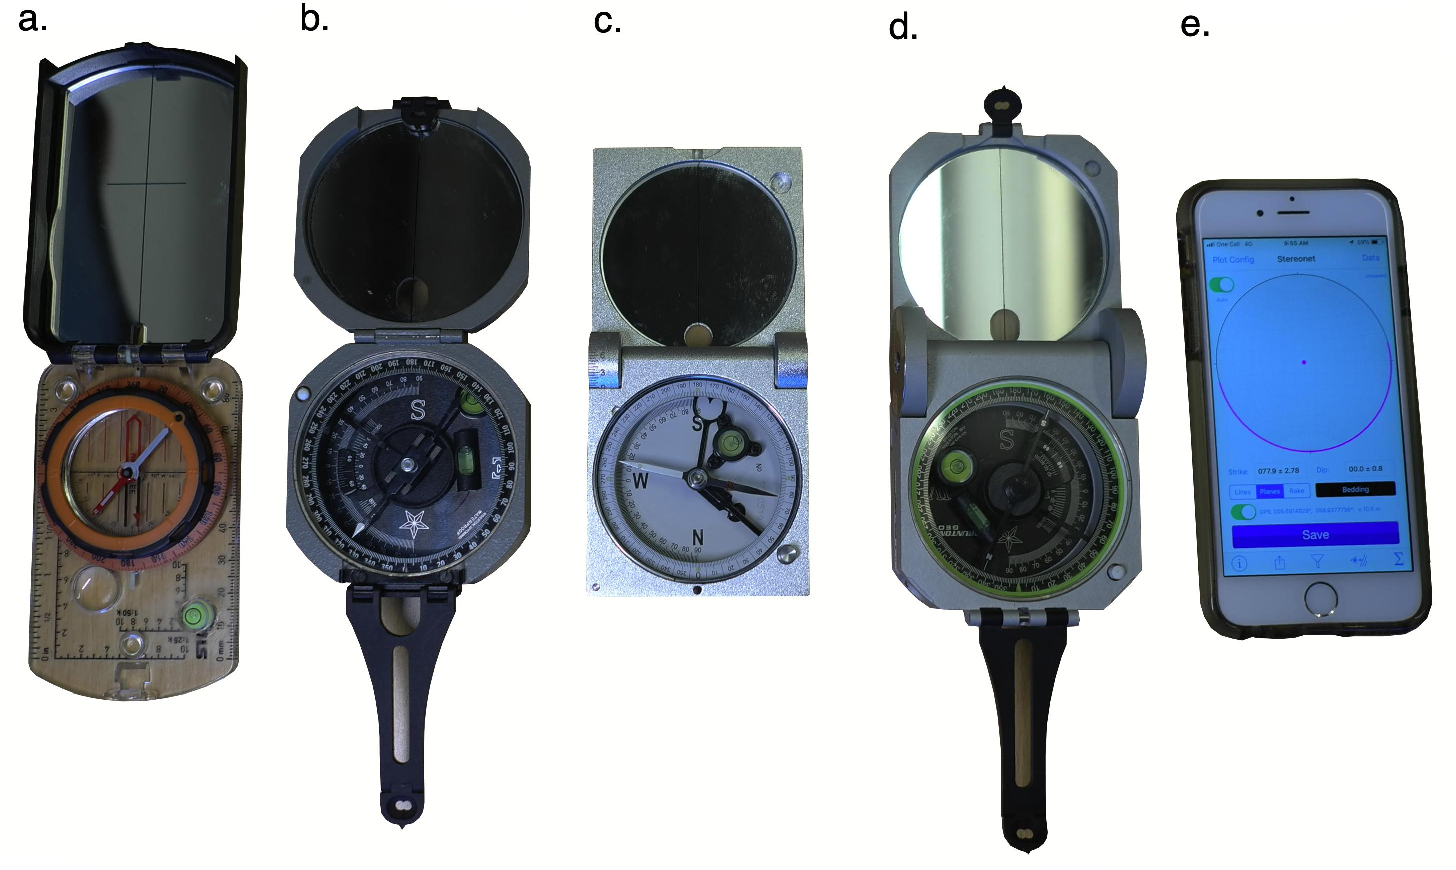
\includegraphics[width=13cm]{ch3f3.pdf}
    \caption{\textbf{a.} Silva, \textbf{b.} Brunton, \textbf{c.} Krantz, \textbf{d.} Brunton Geo, and \textbf{e.} Smartphone with Stereonet Mobile.}
\end{figure}

The Silva and Brunton compasses are designed to measure strike and dip through two measurements, while the Krantz compass measures dip direction and dip at once. The Brunton Geo compass works either as a Brunton or Krantz compass and is more precise than the other compasses (is also more expensive)\footnote{There is even a better compass called the \href{http://www.realscienceinnovations.com/brunton-axis.html}{Brunton axis transit}}. The use of these compasses is explained in field geology books such as Compton (1985) and Coe (2010). Figure 3.4 shows how strike and dip are measured with the Brunton compass. Notice that in this measurement, it is crucial to determine when the compass is horizontal (Fig. 3.4a). This can be a source of error (section 3.2.5).

\begin{figure}[ht]
    \centering
    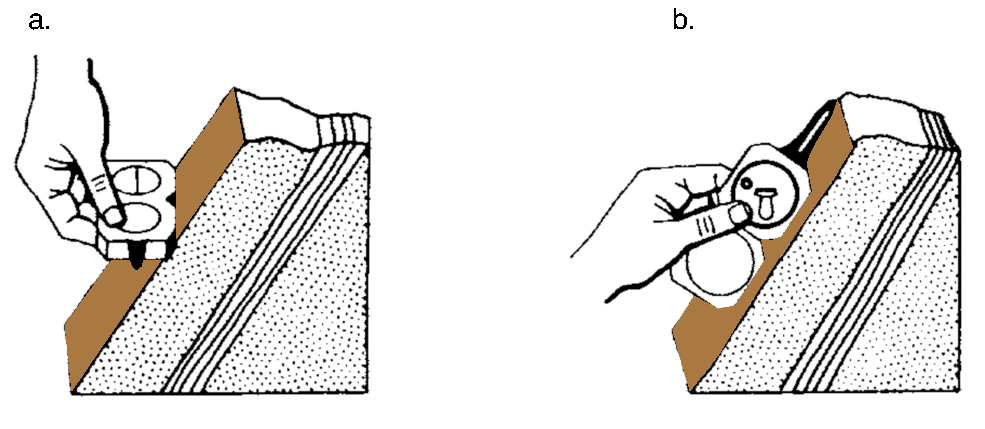
\includegraphics[width=12cm]{ch3f4.pdf}
    \caption{Measuring the \textbf{a.} strike and \textbf{b.} dip of a plane. Modified from Compton (1985).}
\end{figure}

These days, digital devices in the form of smartphone programs or apps (Fig. 3.3e) are slowly replacing the analog compasses. Smartphones contain instruments such as accelerometers, gyroscopes, and magnetometers, which enable apps such as \href{http://www.geo.cornell.edu/geology/faculty/RWA/programs/stereonet-mobile.html}{Stereonet Mobile} (Richard Allmendinger) or \href{https://www.petex.com/products/move-suite/digital-field-mapping/}{Fieldmove Clino} (Petroleum Experts) to determine the exact orientation of the device in space. Measuring a plane or a line just requires placing the phone on the plane or along the line. Thus, one can capture a large number of measurements quickly. However, smartphones are very sensitive to nearby magnetic fields and one can easily get spurious results (Novakova and Plavlis, 2017; Allmendinger et al., 2017; Whitmeyer et al., 2019; Wang et al., 2020). Smartphones also have access to accurate geographic location (GPS, cell and wireless networks) as well as satellite imagery and raster data such as elevation. They can greatly facilitate mapping in the field (Allmendinger et al., 2017).

% SUBSECTION: UNCERTAINTIES
\subsection{Uncertainties in orientations} \label{uncertainties}

Geological planes and lines are irregular and therefore it is difficult to take exact measurements of them. Every plane or line measurement has an uncertainty (an error). There are different ways to try to reduce this error, either by placing a smooth planar object (e.g. a field notebook) on the plane or along the line, or by sighting the plane or line from the distance (Compton, 1985). Figure 3.5 illustrates the error associated to the strike and dip measurement of a plane. If the compass is not exactly horizontal then a direction other than the strike will be measured. The departure of the compass from the horizontal or operator error ($\varepsilon_o$) will give a strike error ($\varepsilon_s$).

\begin{figure}[ht]
    \centering
    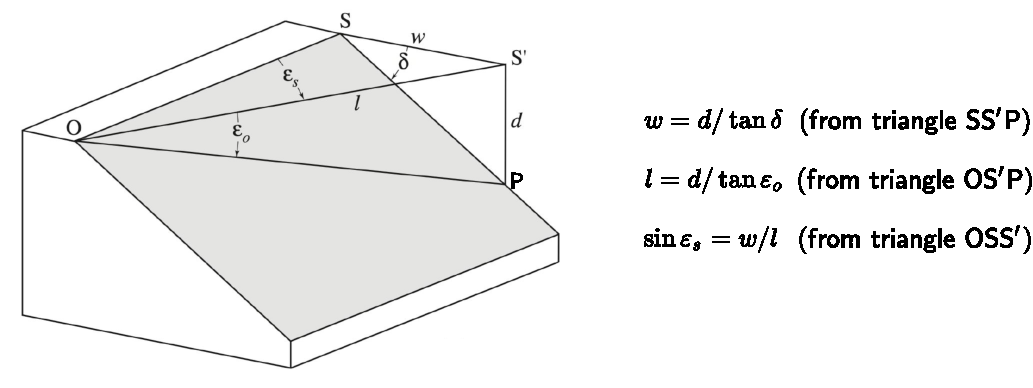
\includegraphics[width=13cm]{ch3f5.pdf}
    \caption{Geometrical relations for estimating the strike error $\varepsilon_s$ from the operator error (or departure of the compass from the horizontal) $\varepsilon_o$.  Modified from Ragan (2009).}
\end{figure}

From the three right-triangles and their corresponding equations in Figure 3.5, and by substituting the first two equations for $w$ and $l$ into the third equation for $\sin\varepsilon_s$, one gets the following relation (Woodcock, 1976):

\begin{equation}
    \sin\varepsilon_s = \frac{\tan\varepsilon_o}{\tan\delta}
\end{equation}

where $\delta$ is the dip angle of the plane. This equation is plotted in Figure 3.6 for dip angles $\delta$ of 0 to 40\degree\space and operator errors $\varepsilon_o$ of 1 to 5\degree. It is clear that the strike error $\varepsilon_s$ increases with decreasing dip. For a gentle 5\degree dipping plane, an operator error $\varepsilon_o$ of 2\degree\space (a compass just 2\degree\space off the horizontal) results in a strike error $\varepsilon_s$ of about 24\degree! Thus, one should always be suspicious about the accuracy of strike and dip measurements, particularly if they are from gently dipping planes.

\begin{figure}[ht]
    \centering
    {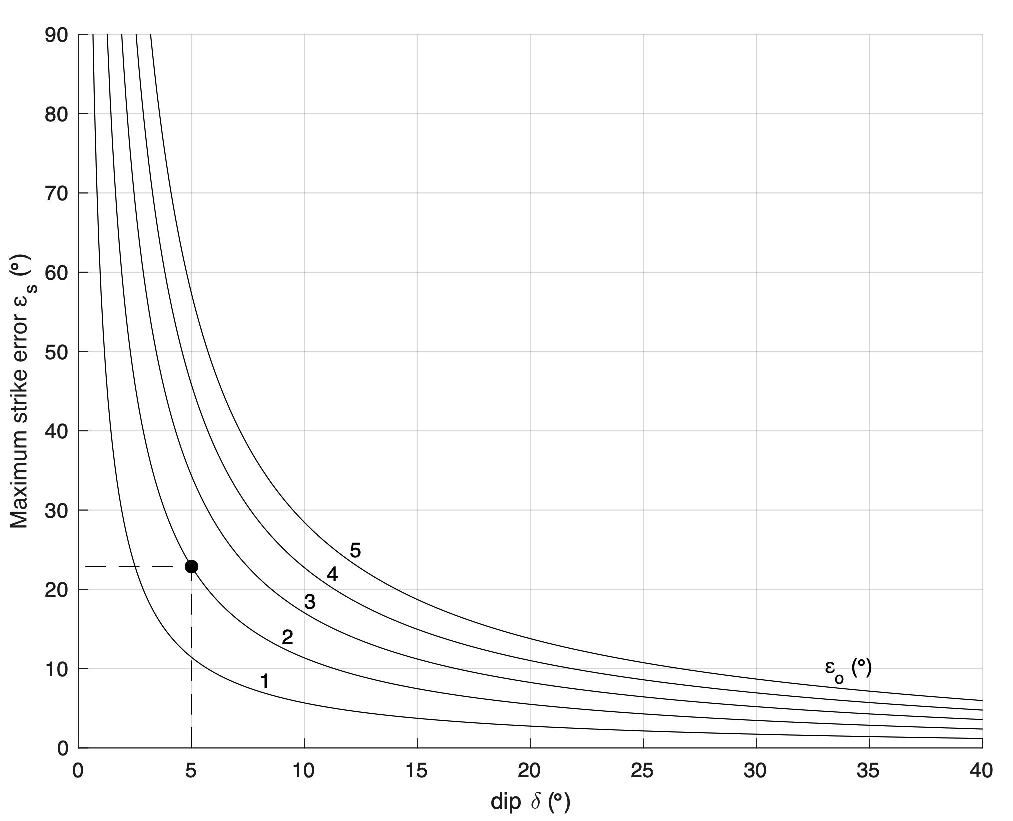
\includegraphics[width=12cm]{ch3f6.pdf}}
    \caption{Strike error $\varepsilon_s$ as a function of dip $\delta$ for values of operator error $\varepsilon_o$  of 1-5\degree. The \href{https://github.com/nfcd/compGeo/blob/master/source/notebooks/ch3-fig6.ipynb}{notebook} that produced this graph is available from the resource git repository.}
\end{figure}

For line measurements, the situation is not better. When measuring the orientation of a line, it is common practice to align the compass in the direction of the horizontal projection of the line, which as anyone who has tried this in the field knows, it is quite difficult. There will be an operator error and the measured trend $\beta\text{$'$}$ will differ from the true trend $\beta$ (Fig. 3.7a). The trend error $\varepsilon_t$ ($|\beta\text{$'$}- \beta|$) in terms of the angle the measured line makes with the true line on the plane $\varepsilon_o$, is given by the following equations (Woodcock, 1976): 

\begin{figure}[ht]
    \centering
    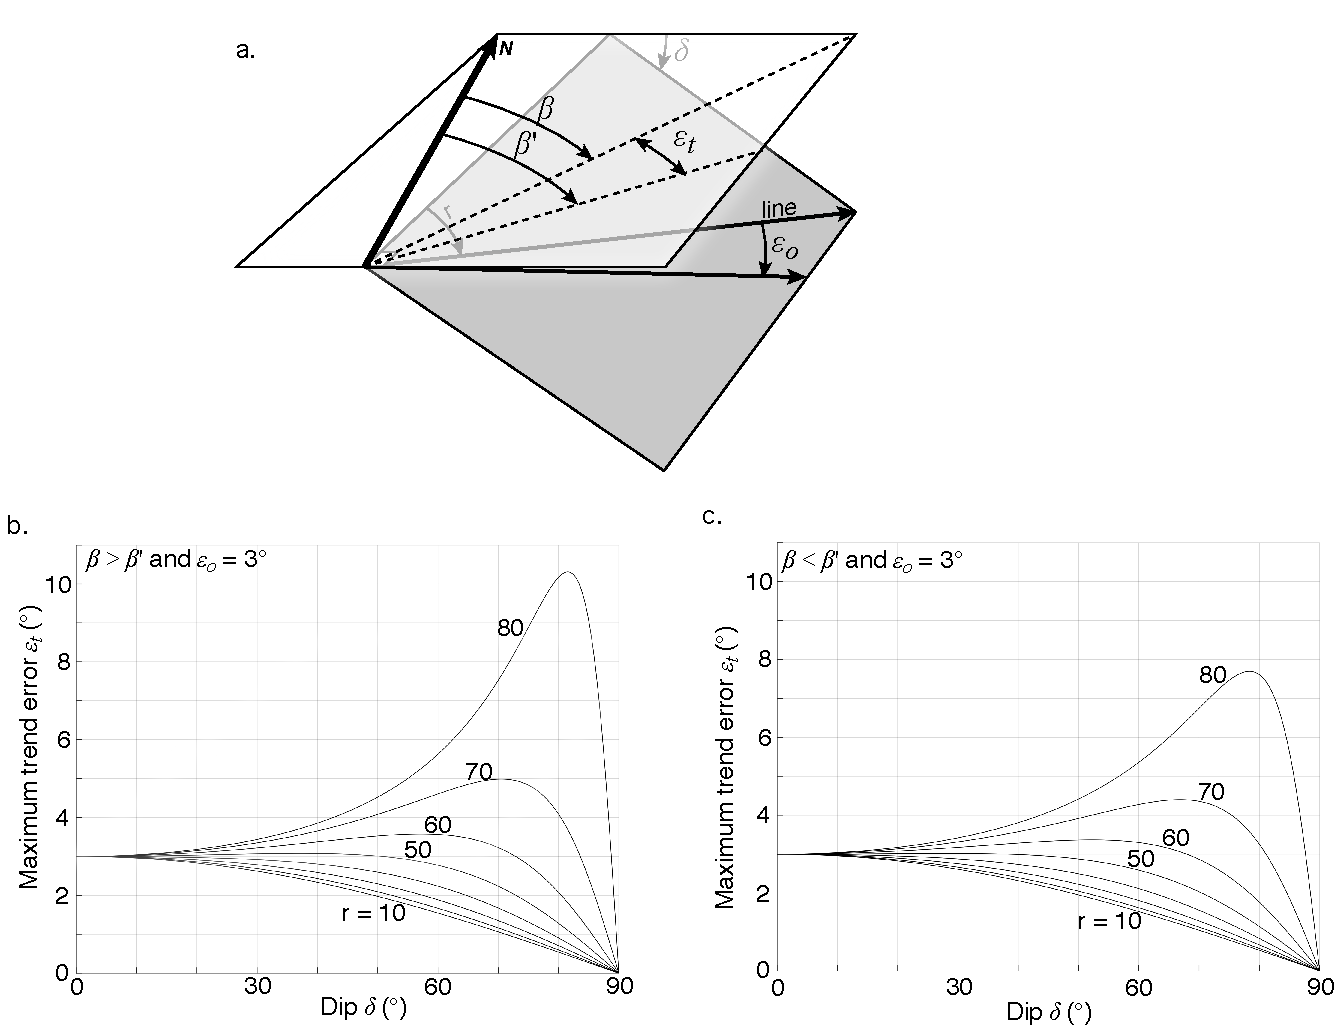
\includegraphics[width=13cm]{ch3f7.pdf}
    \caption{\textbf{a.} Geometrical relations for estimating the trend error $\varepsilon_t$ from the rake $r$ of the line, the dip $\delta$  of the plane, and the angle on the plane $\varepsilon_o$ between the measured and the true lines. \textbf{b.} Measured line on the down-dip side of the line. \textbf{c.} Measured line on the up-dip side of the line. In b and c, $\varepsilon_o$ is 3\degree. Notebooks \href{https://github.com/nfcd/compGeo/blob/master/source/notebooks/ch3-fig7b.ipynb}{b} and \href{https://github.com/nfcd/compGeo/blob/master/source/notebooks/ch3-fig7c.ipynb}{c} produced the graphs.}
\end{figure}

\begin{equation}
    \begin{gathered}
        \tan\varepsilon_t = \frac{[\tan(r+\varepsilon_o)-\tan(r)]\cos\delta}{1+[\tan(r+\varepsilon_o)\tan(r)]\cos^2\delta} \hspace{0.5cm} if \beta\text{$'$}>\beta\\ \\
        \tan\varepsilon_t = \frac{[\tan(r)-\tan(r-\varepsilon_o)]\cos\delta}{1+[\tan(r)\tan(r-\varepsilon_o)]\cos^2\delta} \hspace{0.5cm} if \beta\text{$'$}<\beta
    \end{gathered}
\end{equation}

where $r$ is the rake of the line, and $\delta$ is the dip of the plane (Fig. 3.7a). These equations are plotted in Figure 3.7b-c for an $\varepsilon_o$ of 3\degree. The trend error is greater for a measured line on the down-dip side of the line ($\beta\text{$'$} > \beta$, Fig. 3.7b), than for a measured line on the up-dip side of the line ($\beta\text{$'$} < \beta$, Fig. 3.7c). This means that repeated measurements will not be symmetrically distributed around the true trend $\beta$. Also for a given $\varepsilon_o$, the trend error $\varepsilon_t$ increases with the dip $\delta$ of the plane and the rake $r$ of the line, i.e. a combination of a steep plane and a large rake may result in a large trend error.

Equations 3.3 and 3.4 allow determining the uncertainties associated to the measurement of planes and lines. As we will see in section \ref{calcuncertainties}, these errors propagate in any computation making use of these angles.

% SECTION: DISPLAYING GEOLOGICAL FEATURES
\section{Displaying geological features}

There are two fundamental ways geologists display geological features on a piece of paper: maps and stereonets. In maps, we are concerned about the location and orientation of the features, and the spatial relation of one feature to another. In stereonets, we are just concerned with the orientation of the features.

% SUBSECTION MAPS
\subsection{Maps}

All maps are a projection of surface or subsurface geological features onto a horizontal plane. In section \ref{projections}, we looked at the different methods used to project data from the approximately spherical Earth to a flat surface, and the distortions associated to these methods. Geological features (bedding, faults, the ground surface) are rarely flat, and therefore to display the spatial variation of their elevation (or depth) on maps, we use contours. A contour line is a line joining the points in the map area of equal value for a specific parameter. On a topographic map, for example, contour lines join points of equal elevation on the ground surface. Contour lines should not cross (unless very unusual circumstances) or disappear in the middle of the map (unless the contoured feature is intersected by another feature). If the difference in value between adjacent contours or contour interval is held constant throughout the map, the gradient (rate of change) of the parameter in a given direction is proportional to the spacing of the contour lines: high gradient is represented by closely spaced contours, and low gradient by widely spaced contours. This is expressed by the following relation:

\begin{equation}
    \text{gradient} = \arctan\frac{\text{parameter\,change\,between\,contours}}{\text{map\,distance\,between\,contours}} \tag{3.5a}
\end{equation}

For a topographic map, this relation becomes:

\begin{equation}
    \text{slope\,angle} = \arctan\frac{\text{elevation\,change\,between\,contours}}{\text{map\,distance\,between\,contours}} \tag{3.5b}
\end{equation}

which is why when choosing the path to a high ground area, you should look for the widely spaced contours (unless you are a climber or a goat).

Geological features are rarely isolated, and they usually have different orientations, so we should expect them to intersect. The intersection of two non-parallel planes (e.g. bedding contacts) is a straight line. In chapter 4, we will see how to determine this type of intersection using vector operations. If one of the surfaces is not planar but irregular, the intersection is a curved line which is more difficult to determine. One fundamental mapping problem geology students are early confronted with is the intersection of a planar feature (e.g. bedding or a fault) with the irregular land surface. This is elegantly summarized by the \textit{Rule of V’s} (Fig. 3.8).

\begin{figure}[ht]
    \centering
    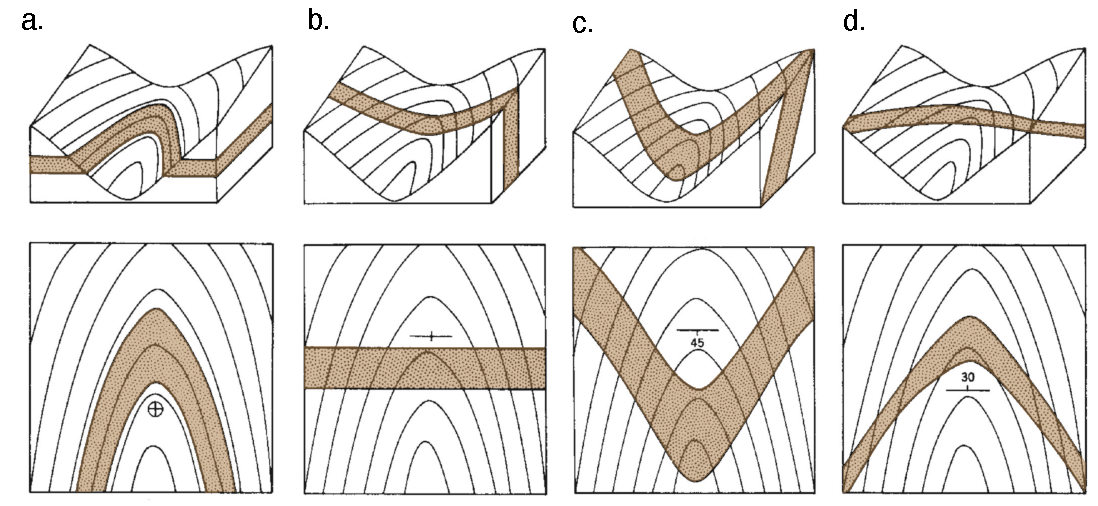
\includegraphics[width=13cm]{ch3f8.pdf}
    \caption{Outcrop pattern across a valley of \textbf{a.} Horizontal bed, \textbf{b.} Vertical bed, \textbf{c.} Bed dipping downstream, and \textbf{d.} Bed dipping upstream. Modified from Ragan (2009).}
\end{figure}

The Rule of V’s says that when a planar contact crosses a valley, its outcrop pattern will V or curve in the direction the contact is dipping, but only if the contact if steeper than the slope of the valley, which is often the case (Fig. 3.8c-d). There are two exceptions: 1. If the contact is horizontal, its outcrop pattern will follow the topographic contours, which makes sense since the contours are the intersection of horizontal planes of different elevation with the ground (Fig. 3.8a), and 2. If the contact is vertical, its outcrop pattern across the valley is a straight line. Vertical planes \textit{ignore} topography.

Determining the outcrop trace of a planar contact on irregular topography is not straightforward. Graphically, this problem involves making elevation contours on the planar contact. These are called structure contours. Then one should look at the location where the structure contours of the contact have the same elevation than the topographic contours of the land surface. On these locations, the contact outcrops. Finally, one should join these locations with a line, to make the outcrop trace of the contact. Figure 3.9 illustrates this procedure for a plane dipping north and intersecting irregular topography. Notice how in the stream valleys, the outcrop trace of the plane curves to the north, clearly following the Rule of V’s.

\begin{figure}[ht]
    \centering
    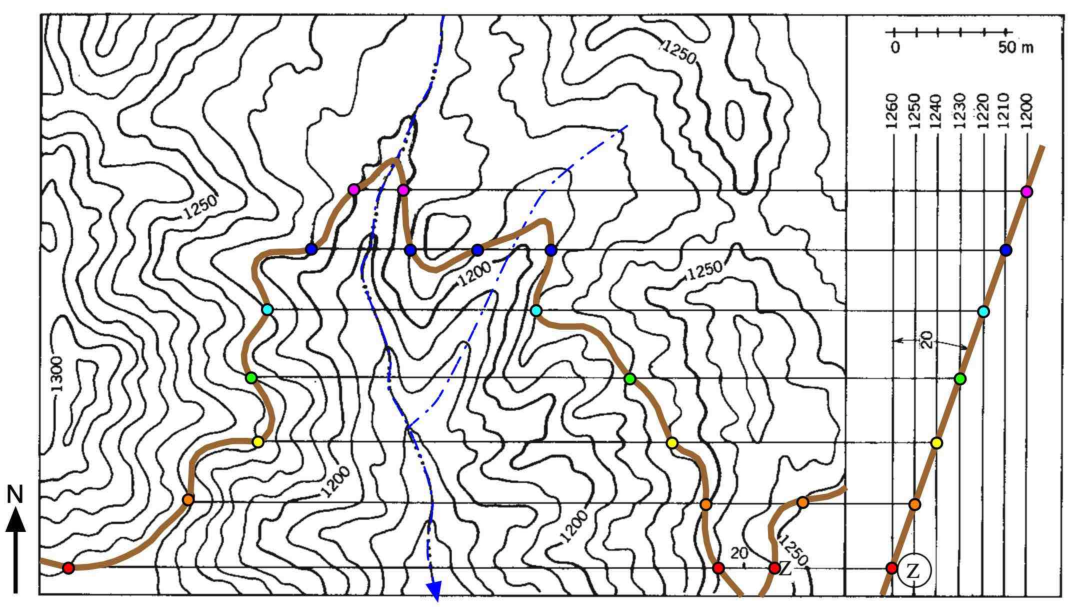
\includegraphics[width=13cm]{ch3f9.pdf}
    \caption{Outcrop trace of a plane dipping 20\degree\space N. The left figure is the map, and the right figure is a N-S cross section. Color points are the locations where the plane's structure contours have the same elevation than the topographic contours. The line joining these points is the outcrop trace of the plane. Modified from Ragan (2009).}
    \label{fig:outrace}
\end{figure}

This graphical approach requires a great deal of patience and drawing skills. Later in section \ref{outcrop}, we sill see that if we know the plane’s orientation and one outcrop location, it is possible to project the plane throughout the terrain using computation, provided we have a digital elevation model (DEM) of the terrain. This saves a lot of time and is a great way to quality control mapping, test different hypotheses, and take better decisions in the field.

% SUBSECTION: STEREONETS
\subsection{Stereonets}

Spherical projections can be used to represent the orientation of a plane or a line, if the plane or line is positioned so that it passes through the center of the sphere. A plane will intersect the sphere along a great circle, and a line will pierce the sphere at a point (Fig. 3.10a). However, it would be inconvenient to carry a sphere everywhere. Fortunately, it is possible to project the sphere onto a plane using, for example, an azimuthal projection (section \ref{projections}).

\begin{figure}[ht]
    \centering
    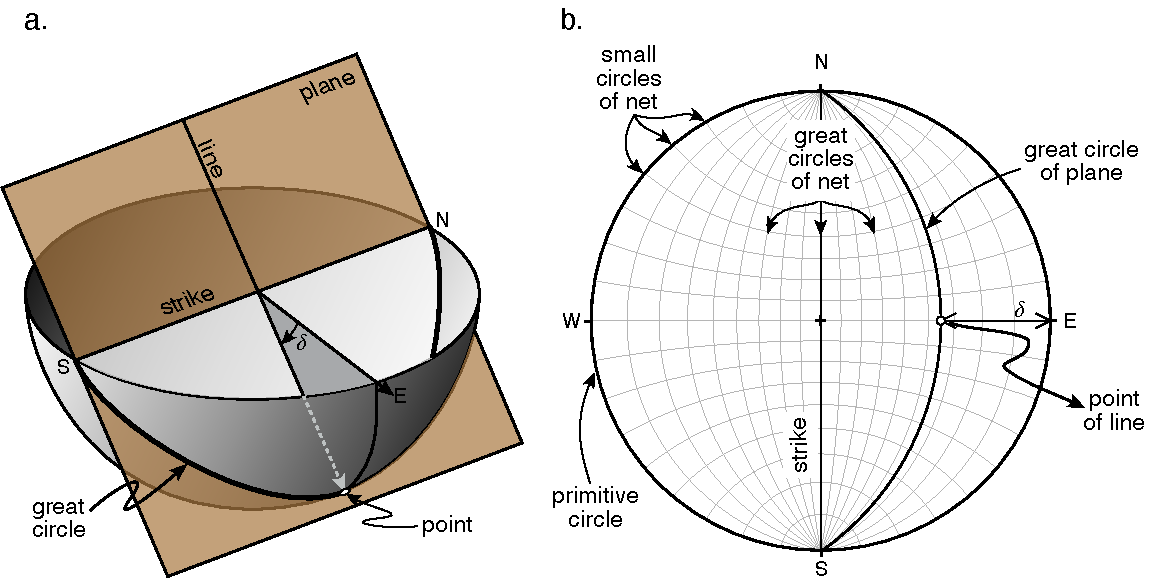
\includegraphics[width=13cm]{ch3f10.pdf}
    \caption{\textbf{a.} Plane and line intersecting the lower half of a sphere. The rake of the line is 90\degree\space and therefore its plunge is equal to the plane’s dip $\delta$. \textbf{b.} Lower hemisphere stereographic projection of plane and line. Modified from Allmendiger et al. (2012) and Allmendinger (2020).}
\end{figure}

A \textit{stereonet} or stereographic projection is a special kind of azimuthal projection, where the point source or viewpoint lies on the surface of the sphere, and the projection plane passes through the center of the sphere. In a stereonet, the viewpoint is at the top of the sphere or zenith, the view direction is downwards, the projection plane is the equatorial plane dividing the sphere into lower and upper hemispheres, and the lower hemisphere (bowl in Fig. 3.10a) is projected. In the stereonet, the rim of the bowl is called the primitive circle and it corresponds to a horizontal plane (Fig. 3.10b). A net facilitates drawing any plane or line. This net consists of great circles representing N-S striking, 0-90\degree\space E and W dipping planes, and small circles representing cones of N-S horizontal axis and 0-90\degree\space apical radius opening to the N and S (Fig. 3.10b). Several books explain the use of the stereonet to solve orientation problems (e.g. Marshak and Mitra, 1988).

For our purpose, it is more important to know how this projection actually works. Figure 3.11a illustrates this on a vertical section passing through the center of the sphere. Any line from the zenith (the top of the sphere) pinches the equatorial plane at one point, and this is the location where the point plots in the stereonet. This is defined by the following equation:

\begin{figure}[ht]
    \centering
    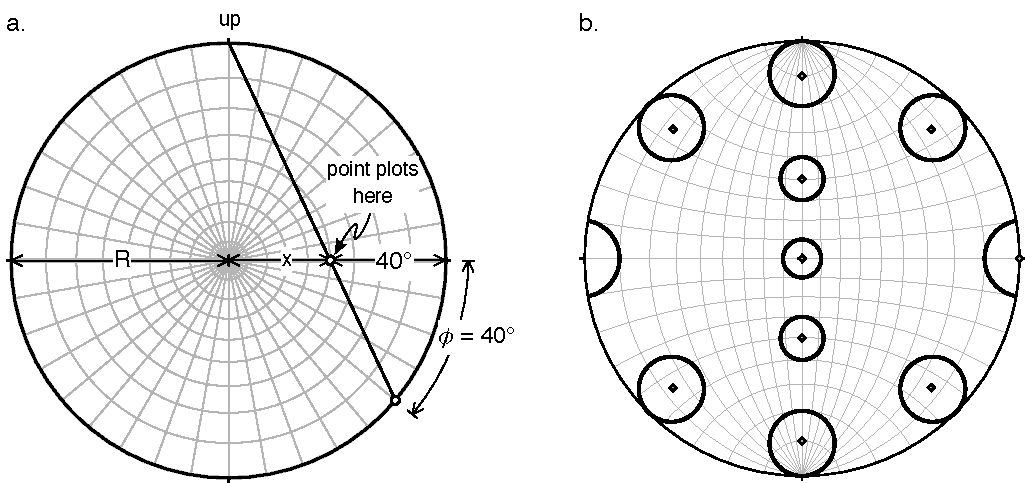
\includegraphics[width=13cm]{ch3f11.pdf}
    \caption{\textbf{a.} The equal angle stereonet illustrated on a vertical plane passing through the center of the sphere. \textbf{b.} Lower hemisphere equal angle projection of small circles of 10\degree\space radius but different axis orientations. Modified from Allmendinger et al. (2012).}
\end{figure}

\begin{equation}
    x = R\tan\left(45\degree-\frac{\phi}{2}\right) \tag{3.6}
\end{equation}

where $x$ is the is the distance of the point from the center of the net, $R$ is the radius of the net, and $\phi$ is the plunge of the line. This method preserves angles perfectly and thus, on the primitive circle, degrees are equally spaced, and a small circle will be a circle anywhere on the net (Fig. 3.11b). This is why this projection is called the equal angle or Wulff stereonet. However, the preservation of angles has a disadvantage: areas are distorted. Thus, for example, a 10\degree\space radius small circle will look smaller near the center of the net but larger near the edges (Fig. 3.11b). This poses a problem when trying to visually evaluate the density of points plotted on the net.

The equal area or Schmidt net (Fig. 3.12) overcomes this problem. Strictly speaking, this projection is not a stereographic projection because the projection plane is at the bottom of the sphere. The point of intersection of the line and the surface of the lower hemisphere is projected to the horizontal plane at the bottom of the sphere, along a circular arc centered at the lowest point of the sphere. The $x$ distance of the point is then scaled by a factor of $\sqrt{2}$ to fit it to the radius $R$ of the net (Fig. 3.12a). This is expressed by the following equation:

\begin{figure}[ht]
    \centering
    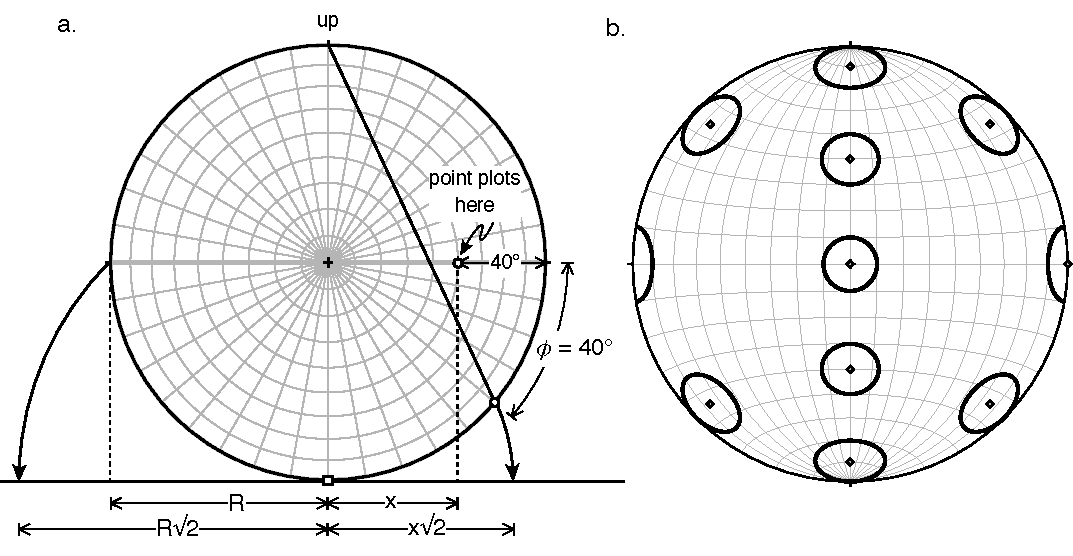
\includegraphics[width=13cm]{ch3f12.pdf}
    \caption{ \textbf{a.} The equal area stereonet illustrated on a vertical plane passing through the center of the sphere. \textbf{b.} Lower hemisphere equal area projection of small circles of 10\degree\space radius but different axis orientations. Modified from Allmendinger et al. (2012).}
\end{figure}

\begin{equation}
    x = R\sqrt{2}\sin\left(45\degree-\frac{\phi}{2}\right) \tag{3.7}
\end{equation}

The tradeoff is that although areas are preserved, angles are no longer preserved, and small circles are no longer true circles (Fig. 3.12b). The equal angle or Wulff net is used for problems where visualizing angles on the net is important such as in crystallography and geography, while the equal area or Schmidt net is used for problems where analyzing the concentration of points on the net is important such as in structural analysis.

The function \href{https://github.com/nfcd/compGeo/blob/master/source/functions/st_coord_line.py}{st\_coord\_line} computes the coordinates of a line in an equal angle or an equal area net (Eqs. 3.7 and 3.8).  Notice that angles (\code{trd} and \code{plg}) should be entered in radians.

\begin{center}
\begin{lstlisting}[language=Python, frame=single]
import math
from zero_twopi import zero_twopi

def st_coord_line(trd,plg,stype):
	"""
	st_coord_line computes the coordinates of a line
	in an equal angle or equal area stereonet of unit radius
	
	trd = trend of line
	plg = plunge of line
	stype = Stereonet type: 0 = equal angle, 1 = equal area
	xp and yp: Coordinates of the line in the stereonet
	
	NOTE: trend and plunge should be entered in radians
	
	Python function translated from the Matlab function
	StCoordLine in Allmendinger et al. (2012)
	"""
	# Take care of negative plunges
	if plg < 0:
		trd = zero_twopi(trd+math.pi)
		plg = -plg
	
	# Some constants
	pis4 = math.pi/4
	s2 = math.sqrt(2)
	plgs2 = plg/2
	
	# Equal angle stereonet
	if stype == 0:
		xp = math.tan(pis4 - plgs2)*math.sin(trd)
		yp = math.tan(pis4 - plgs2)*math.cos(trd)
	# Equal area stereonet
	elif stype == 1:
		xp = s2*math.sin(pis4 - plgs2)*math.sin(trd)
		yp = s2*math.sin(pis4 - plgs2)*math.cos(trd)
	
	return xp, yp
\end{lstlisting}   
\end{center}

% SUBSECTION: PLOTTING LINES AND POLES IN THE STEREONETS
\subsection{Plotting lines and poles in a stereonet}
The notebook \href{https://github.com/nfcd/compGeo/blob/master/source/notebooks/ch3.ipynb}{ch3} illustrates the use of the \code{st\_coord\_line} function to plot lines and poles to planes on an equal angle or equal area stereonet. Notice that for planes, we use the \code{pole\_from\_plane} function to compute the pole to the plane. You will get the chance to practice more with these functions in section \ref{exercises3}.

\begin{center}
\begin{lstlisting}[language=Python, frame=single]
# Import libraries
import numpy as np
import matplotlib.pyplot as plt

# Import functions pole_from_plane and
# st_coord_line
import sys, os
sys.path.append(os.path.abspath("../functions"))
from pole import pole_from_plane
from st_coord_line import st_coord_line

# Make a figure
fig, ax = plt.subplots()

# Plot the following four lines (trend and plunge)
# on an equal angle or equal area stereonet
# lines are in radians
lines = np.radians([[30, 30],[120, 45],[210, 65],[280, 15]])

# Plot the primitive of the stereonet
r = 1; # unit radius
th = np.radians(np.arange(0,361,1))
x = r * np.cos(th)
y = r * np.sin(th)
ax.plot(x,y,"k")
# Plot center of circle
ax.plot(0,0,"k+")
# Make axes equal and remove them
ax.axis("equal")
ax.axis("off")

# Find the coordinates of the lines in the
# equal angle or equal area stereonet
nrow, ncol = lines.shape
eq_angle = np.zeros((nrow, ncol))
eq_area = np.zeros((nrow, ncol))

for i in range(nrow):
    # Equal angle coordinates
    eq_angle[i,0], eq_angle[i,1] = st_coord_line(lines[i,0],
                                    lines[i,1],0) 
    # Equal area coordinates
    eq_area[i,0], eq_area[i,1] = st_coord_line(lines[i,0],
                                    lines[i,1],1)
    
# Plot the lines
# Equal angle as black dots
ax.plot(eq_angle[:,0],eq_angle[:,1],"ko")
# Equal area as red dots
ax.plot(eq_area[:,0],eq_area[:,1],"ro");
\end{lstlisting}
\fbox{
\parbox{\textwidth - 2 \fboxsep}{
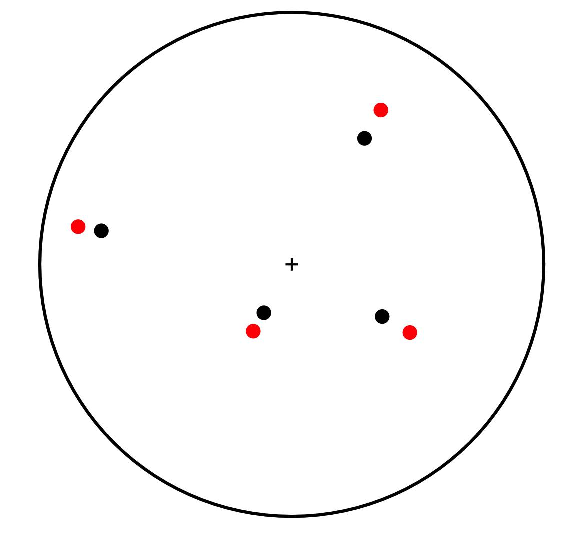
\includegraphics[width=5cm]{ch3f13.pdf}
}}
\end{center}

\begin{center}
\begin{lstlisting}[language=Python, frame=single]
# Plot the following four planes (strike and dip, RHR)
# as poles on an equal angle or equal area stereonet
# planes are in radians
planes = np.radians([[0, 30], [90, 50], 
                     [180, 15], [270, 65]])

# make a figure
fig, ax = plt.subplots()

# Plot the primitive of the stereonet
ax.plot(x,y,"k")
# Plot center of circle
ax.plot(0,0,"k+")
# Make axes equal and remove them
ax.axis("equal")
ax.axis("off")

# Find the coordinates of the poles to the planes in the
# equal angle or equal area stereonet
for i in range(nrow):
    # Compute pole of plane
    trd, plg = pole_from_plane(planes[i,0],planes[i,1])
    # Equal angle coordinates
    eq_angle[i,0], eq_angle[i,1] = st_coord_line(trd,plg,0) 
    # Equal area coordinates
    eq_area[i,0], eq_area[i,1] = st_coord_line(trd,plg,1)

# Plot the poles
# Equal angle as black asterisks
ax.plot(eq_angle[:,0],eq_angle[:,1],"k*")
# Equal area as red asterisks
ax.plot(eq_area[:,0],eq_area[:,1],"r*");
\end{lstlisting}
\fbox{
\parbox{\textwidth - 2 \fboxsep}{
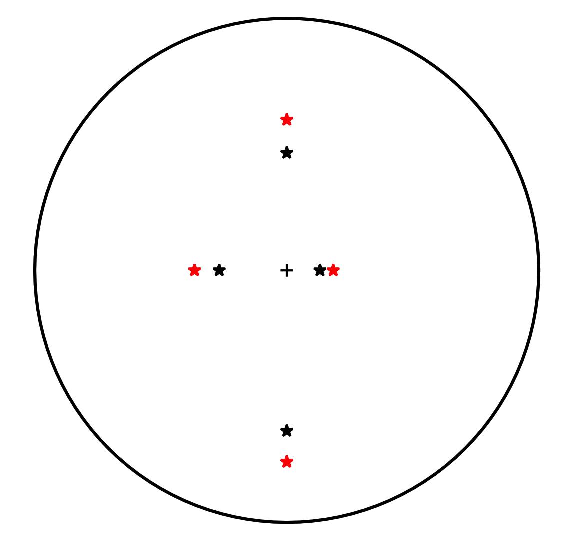
\includegraphics[width=5cm]{ch3f14.pdf}
}}
\end{center}

% SECTION: EXERCISES
\section{Exercises} \label{exercises3}

\begin{enumerate}
  \item Modify the notebook that makes Fig. 3.6 to extend the range of dip $\delta$ angles from 0 to 90\degree\space and the operator error $\varepsilon_o$ from 1 to 10\degree.
  
  \item Modify the notebooks that make Fig. 3.7 b and c for an $\varepsilon_o$ of 5\degree.
  
  \item A great circle on a stereonet can be drawn by plotting closely spaced points along the great circle. These are lines on the plane. The following arrays contain the trend and plunge of lines on a plane of orientation 030/40 (strike and dip, RHR format):
  
  trend = [30, 34, 38, 42, 46, 50, 54, 58, 63, 67, 72, 78, 83, 89, 95, 101, 107, 113, 120, 127, 133, 139, 145, 151, 157, 162, 168, 173, 177, 182, 186, 190, 194, 198, 202, 206, 210]
  
  plunge = [0, 3, 6, 10, 13, 16, 19, 22, 24, 27, 29, 32, 34, 36, 37, 38, 39, 40, 40, 40, 39, 38, 37, 36, 34, 32, 29, 27, 24, 22, 19, 16, 13, 10, 6, 3, 0]
  
  Plot these lines on an equal angle and an equal area stereonet using the function \code{st\_coord\_line}. Don't use a stereonet program, we will implement one in Chapter 5.
  
  \item A small circle on a stereonet can be drawn by plotting closely spaced points along the small circle. These are lines on the conical surface. The following arrays contain the trend and plunge of lines on a small circle of axis 050/30 (trend and plunge) and radius 20\degree:
  
  trend = [50, 53, 57, 60, 63, 66, 68, 70, 72, 73, 73, 73, 72, 70, 68, 64, 60, 55, 50, 45, 40, 36, 32, 30, 28, 27, 27, 27, 28, 30, 32, 34 37, 40, 43, 47, 50]
  
  plunge = [10, 10, 11, 12, 14, 16, 19, 22, 25, 28, 31, 35, 38, 41, 44, 47, 48, 50, 50, 50, 48, 47, 44, 41, 38, 35, 31, 28, 25, 22, 19, 16 14, 12, 11, 10, 10]
  
  Plot these lines on an equal angle and an equal area stereonet using the function \code{st\_coord\_line}. What are the differences between the small circles in the equal angle and equal area stereonets? 
  
  \item The strike and dip arrays below contain the strike and dip (RHR format) of 50 bedding planes in a fold:
  
  strike = [8, 22, 19, 33, 27, 37, 41, 47, 55, 40, 32, 55, 65, 68, 89, 79, 102, 105, 108, 122, 132, 136, 145, 159, 156, 164, 176, 169, 179, 173, 167, 160, 145, 148, 141, 125, 108, 92, 75, 57, 50, 39, 22, 10, 1, 9, 15, 16, 114, 78]
  
  dip = [75, 79, 68, 72, 61, 46, 50, 67, 51, 66, 55, 42, 49, 58, 54, 45, 35, 49, 63, 45, 52, 66, 52, 59, 76, 64, 72, 83, 78, 88, 72, 81, 73, 62, 50, 63, 42, 48, 56, 62, 50, 65, 76, 87, 81, 68, 74, 83, 56, 37]
  
  Plot the poles to these planes in an equal area stereonet using the functions \code{pole\_from\_plane} and \code{st\_coord\_line}. The resultant diagram is called a $\pi$- diagram. What is the approximate orientation of the great circle defined by the poles? What does the pole to this great circle represent? 
  
\end{enumerate}

% SECTION: REFERENCES
\addcontentsline{toc}{section}{References}
\section*{References}

Allmendinger, R.W., Cardozo, N. and Fisher, D.W. 2012. Structural Geology Algorithms: Vectors and Tensors. Cambridge University Press.

Allmendinger, R.W., Siron, C.R. and Scott, C.P. 2017. Structural data collection with mobile devices: Accuracy, redundancy,and best practices. Journal of Structural Geology 102, 98-112.

Allmendinger, R.W. 2020. Modern Structural Practice: A structural geology laboratory manual for the 21st century. [\href{https://www.rickallmendinger.net/download}{Online}]. [Accessed March, 2021].

Coe, A. 2010. Geological Field Techniques. Wiley-Blackwell.

Compton, R.R. 1985. Geology in the field. John Wiley \& Sons.

Novakova, L. and Pavlis, T.L. 2017. Assessment of the precision of smart phones and tablets for measurement of planar orientations: A case study. Journal of Structural Geology 97, 93-103.

Marshak, S. and Mitra, G. 1988. Basic Methods of Structural Geology. Prentice Hall.

Ragan, D.M. 2009. Structural Geology: An Introduction to Geometrical Techniques. Cambridge University Press.

Wang, J., Nengpan, J., Chaoyang, H., Junchao, C. and Zheng, D. 2020. Assessment of the accuracy of several methods for measuring the spatial attitude of geological bodies using an android smartphone. Journal of Structural Geology 136, 104393.

Whitmeyer, S.J., Pyle, E.J., Pavlis, T.L, Swanger, W. and Roberts, L. 2019. Modern approaches to field data collection and mapping: Digital methods, crowdsourcing, and the future of statistical analyses. Journal of Structural Geology 125, 29-40.

Woodcock, N.H. 1976. The accuracy of structural field measurements. Journal of Geology 84, 350-355.

% CHAPTER 4: COORDINATE SYSTEMS AND VECTORS
\chapter{Coordinate systems and vectors}

Strike and dip, and trend and plunge, are a convenient way to represent the orientation of planes and lines. However, it is difficult to handle these measurements using computation. In this chapter, we will see how to convert linear features (lines and poles to planes) from spherical (trend and plunge) to Cartesian (direction cosines) coordinates, thus representing these features as vectors. This facilitates the analysis of planes and lines using linear algebra and computation, and it will allow us to solve a range of interesting problems using vector operations.

% SECTION: Coordinate systems
\section{Coordinate systems}

Any point or location in space can be represented by the coordinates of the point with respect to the three orthogonal axes of a Cartesian coordinate system. We will call the axes of this coordinate system $\mathbf{X_1}$, $\mathbf{X_2}$ and $\mathbf{X_3}$ (Fig. 4.1). In addition, we will follow a right-handed naming convention: If you hold your right hand so that your thumb points in the positive direction of the first axis $\mathbf{X_1}$, your other fingers should curl from the positive direction of the second axis $\mathbf{X_2}$ toward the positive direction of the third axis $\mathbf{X_3}$ (Fig. 4.1). Such a coordinate system is called a right-handed coordinate system.

In geosciences, we use mainly two types of right-handed coordinate systems: An east (\textbf{E}), north (\textbf{N}), up (\textbf{U}) coordinate system (Fig. 4.1a), and a north (\textbf{N}), east (\textbf{E}), down (\textbf{D}) coordinate system (Fig. 4.1b). The \textbf{ENU} coordinate system is used in GIS and Geophysics when dealing with elevations (e.g. topography), while the \textbf{NED} coordinate system is used in Structural Geology where, by convention, angles measured downwards from the horizontal (e.g. plunge of a downward pointing line) are considered positive. In this chapter, we will use mainly the \textbf{NED} coordinate system, but when dealing with topography and elevations, we will use the \textbf{ENU} coordinate system.

\begin{figure}[ht]
    \centering
    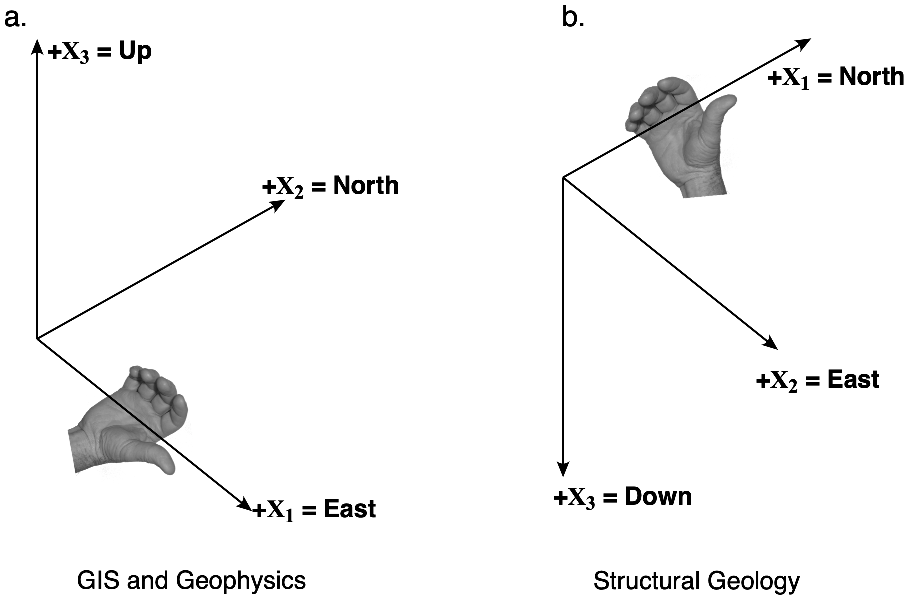
\includegraphics[width=13cm]{ch4f1.pdf}
    \caption{Right-handed Cartesian coordinate systems. \textbf{a.} The \textbf{ENU} coordinate system used when dealing with topography, and \textbf{b.} The \textbf{NED} coordinate system used in Structural Geology. Modified from Allmendinger et al. (2012).}
\end{figure}

% SECTION: VECTORS
\section{Vectors}

\subsection{Vector components, magnitude, and unit vectors}
A line from the origin of the Cartesian coordinate system to a point in space is the position vector of the point. A \textit{vector} is an object that has both a magnitude and a direction. Displacement, velocity, force, acceleration, and poles to planes, are all vectors. A vector is defined by its three components with respect to the axes of the Cartesian coordinate system; these are the projections of the vector onto the axes $\mathbf{X_1}$, $\mathbf{X_2}$ and $\mathbf{X_3}$ (Fig. 4.2a).

\begin{figure}[ht]
    \centering
    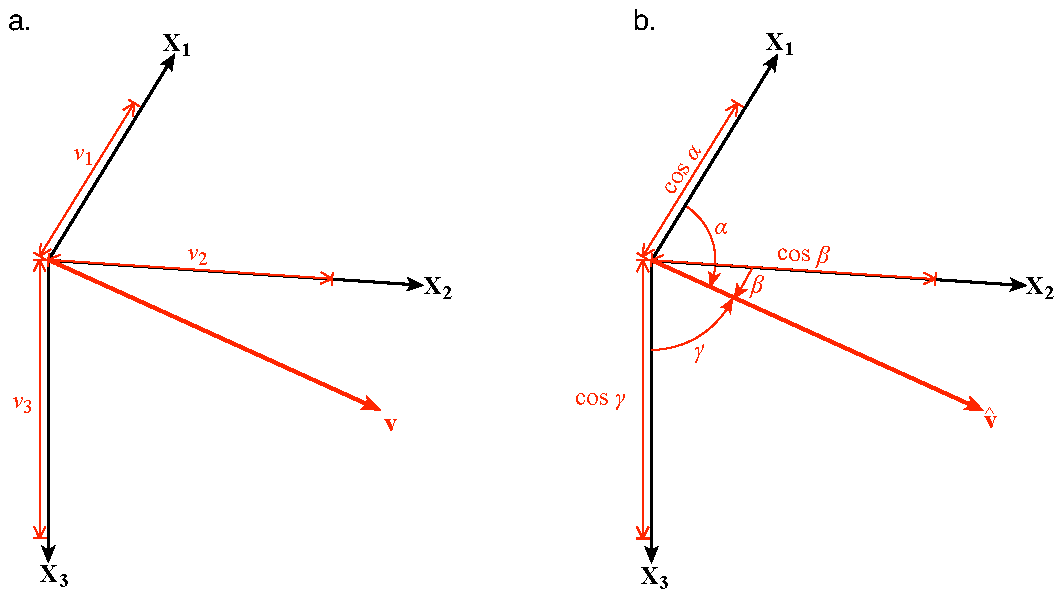
\includegraphics[width=13cm]{ch4f2.pdf}
    \caption{\textbf{a.} Components of a vector. \textbf{b.} Direction cosines of a unit vector. Modified from Allmendinger et al. (2012)}
\end{figure}

This is expressed by the following equation:

\begin{equation}
    \mathbf{v} = [v_1,v_2,v_3]
\end{equation}

We use lower capital, bold letters to denote vectors. The magnitude (length) of a vector can be computed using Pythagoras' theorem:
\begin{equation}
    v = (v_1^2+v_2^2+v_3^2)^{1/2}
\end{equation}

The result is just a number or scalar. We use regular, non-capital letters to denote scalars. If we divide each of the components of a vector by its magnitude, the result is a unit vector, a vector with the same orientation but with a magnitude (length) of one (Fig. 4.2b):

\begin{equation}
    \mathbf{\hat{v}}=[v_1/v,v_2/v,v_3/v]
\end{equation}

We use a hat to indicate unit vectors. There is a very interesting property of unit vectors; the components of a unit vector are the cosines of the angles the vector makes with the axes of the coordinate system (Fig. 4.2b):

\begin{equation}
    \mathbf{\hat v} = [\cos\alpha,\cos\beta,\cos\gamma]
\end{equation}

these are called the \textit{direction cosines} of the vector. By convention, $\cos\alpha$ is the direction cosine of the vector with respect to $\mathbf{X_1}$, $\cos\beta$ is the direction cosine of the vector with respect to $\mathbf{X_2}$, and $\cos\gamma$ is the direction cosine of the vector with respect to $\mathbf{X_3}$ (Fig. 4.2b).

In Python, we can use the NumPy \code{linalg.norm} function to compute the magnitude of a vector, and convert the vector to a unit vector as illustrated in the following notebook \href{https://github.com/nfcd/compGeo/blob/master/source/notebooks/ch4-1.ipynb}{ch4-1}:

\begin{center}
\begin{lstlisting}[language=Python, frame=single]
# Import numpy
import numpy as np
# Import linear algebra functions
from numpy import linalg as la
# Make vector
v = np.array([1,2,3])
print("Vector:", v)
# Magnitude of the vector
length = la.norm(v) 
print("Magnitude of the vector:", length)
# Unit vector
v_hat = v / length
print("Unit Vector:", v_hat)
# Magnitude of unit vector
length = la.norm(v_hat) 
print("Magnitude of the unit vector:", length)
\end{lstlisting}
\fbox{
\parbox{\textwidth - 2 \fboxsep}{
Vector: [1 2 3] \\
Magnitude of the vector: 3.7416573867739413 \\
Unit Vector: [0.26726124 0.53452248 0.80178373] \\
Magnitude of the unit vector: 1.0
}}   
\end{center}

\subsection{Vector operations}
To multiply a scalar times a vector, just multiply each component of the vector by the scalar:

\begin{equation}
    x\mathbf v=[xv_1,xv_2,xv_3]
\end{equation}

This operation is useful, for example, to reverse the direction of a vector; just multiply the vector by -1.
To add two vectors, just sum their components:

\begin{equation}
    \mathbf u + \mathbf v=\mathbf v+\mathbf u=[u_1+v_1,u_2+v_2,u_3+v_3]
\end{equation}

Vector addition is commutative but vector subtraction is not. Vector addition and subtraction obey the parallelogram rule, whereby the resulting vector bisects the two vectors to be added or subtracted (Fig. 4.3a).

\begin{figure}[ht]
    \centering
    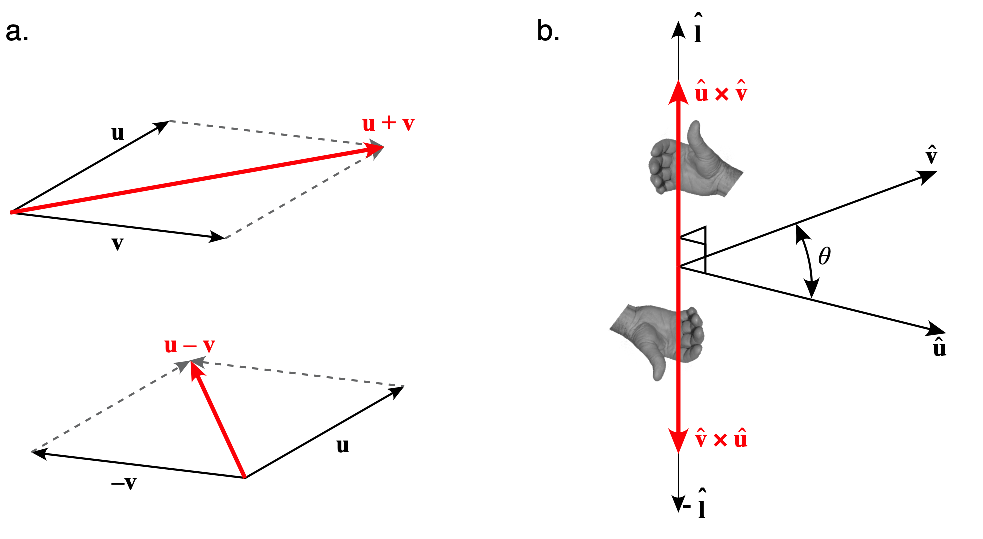
\includegraphics[width=13cm]{ch4f3.pdf}
    \caption{\textbf{a.} Vector addition and subtraction. \textbf{b.} Cross product of two unit vectors. Modified from Allmendinger et al. (2012).}
\end{figure}

There are two operations that are unique to vectors: the \textit{dot product} and the \textit{cross product}. The result of the dot product is a scalar and is equal to the magnitude of the first vector times the magnitude of the second vector times the cosine of the angle between the vectors:

\begin{equation}
    \mathbf u \cdot\mathbf v=\mathbf v \cdot\mathbf u=uv\cos\theta=u_1v_1+u_2v_2+u_3v_3=u_iv_i
\end{equation}

The dot product is commutative. If the two vectors are unit vectors, you can easily see that the dot product is the cosine of the angle between the vectors:

\begin{equation}
    \mathbf{\hat u} \cdot\mathbf{\hat v}=\cos\theta=u_1v_1+u_2v_2+u_3v_3
\end{equation}

or in terms of the direction cosines of the vectors:

\begin{equation}
    \mathbf{\hat u} \cdot\mathbf{\hat v}=\cos\theta=cos\alpha_1\cos\alpha_2+\cos\beta_1\cos\beta_2+\cos\gamma_1\cos\gamma_2
\end{equation}

which as we will see later, it is a great way to find the angle between two unit vectors.

The result of the cross product is another vector. This vector is perpendicular to the other two vectors, and it has a magnitude equal to the product of the magnitudes of the vectors times the sine of the angle between the vectors:

\begin{equation}
    \mathbf u\times\mathbf v=uv\sin\theta\mathbf{\hat l}=[u_2v_3-u_3v_2,u_3v_1-u_1v_3,u_1v_2-u_2v_1]
\end{equation}

The cross product is not commutative. If the vectors are unit vectors, the length of the resulting vector is equal to the sine of the angle between the vectors (Fig. 4.3b). The new vector obeys a right-hand rule; for $\mathbf u\times\mathbf v$, the fingers curl from $\mathbf u$ towards $\mathbf v$ and the thumb points in the direction of the resulting vector, and vice versa (Fig. 4.3b).

In Python, these operations are easy to perform using the NumPy library as shown in the following notebook \href{https://github.com/nfcd/compGeo/blob/master/source/notebooks/ch4-2.ipynb}{ch4-2}:

\begin{center}
\begin{lstlisting}[language=Python, frame=single]
# Import numpy
import numpy as np
# Make vectors
u = np.array([1,2,3])
v = np.array([3,2,1])
print("u =", u)
print("v =", v)
# Scalar multiplication of vector
sv = 3 * u
print("3 * u =", sv)
# Sum of vectors
vsum = u + v
print("u + v =", vsum)
#  Dot product of vectors
dotp = np.dot(u,v)
print("u . v =", dotp)
# Cross product of vectors
crossp = np.cross(u,v) 
print("u x v =", crossp)
\end{lstlisting}
\fbox{
\parbox{\textwidth - 2 \fboxsep}{
u = [1 2 3] \\
v = [3 2 1] \\
3 * u = [3 6 9] \\
u + v = [4 4 4] \\
u . v = 10 \\
u x v = [-4  8 -4]
}}   
\end{center}

% SECTION: GEOLOGICAL FEATURES AS VECTORS
\section{Geological features as vectors}

We have now all the mathematical tools needed to represent geological features as vectors. Since we are only interested in the orientation of these features, we will treat lines (and poles to planes) as unit vectors. We will also use the Structural Geology \textbf{NED} coordinate system.

\subsection{From spherical to Cartesian coordinates}

Figure 4.4 shows a line as a unit vector $\mathbf{\hat{v}}$ in the \textbf{NED} coordinate system. Clearly, the angle that the line makes with the \textbf{D} axis is $90\degree - \textit{plunge}$, therefore:

\begin{figure}[ht]
    \centering
    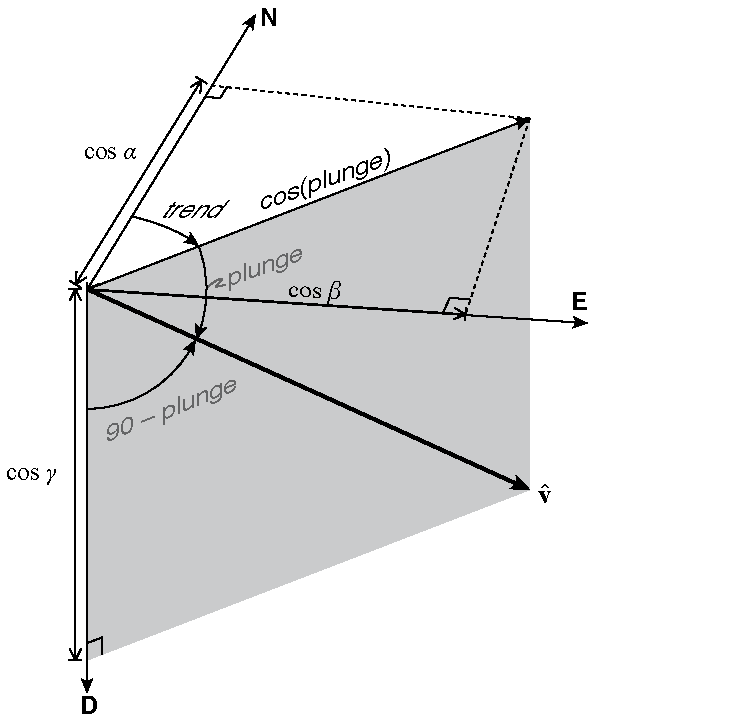
\includegraphics[width=10cm]{ch4f4.pdf}
    \caption{Diagram showing the relations between the trend and plunge and the direction cosines in the \textbf{NED} coordinate system. Gray plane is the vertical plane in which the plunge is measured. Modified from Allmendinger et al. (2012).}
\end{figure}

\begin{equation}
    \cos\gamma=\cos(90\degree-plunge)=\sin(plunge) \tag{4.11a}
\end{equation}

The horizontal projection of the line is $\cos(plunge)$ (Fig. 4.4). $\cos\alpha$ and $\cos\beta$ are just the \textbf{N} and \textbf{E} components of this horizontal line (Fig. 4.4):

\begin{equation}
    \cos\alpha=\cos(trend)\cos(plunge) \tag{4.11b}
\end{equation}

\begin{equation}
    \cos\beta=\cos(90\degree-trend)\cos(plunge)=\sin(trend)\cos(plunge) \tag{4.11c}
\end{equation}

\newpage
Table 4.1 summarizes these equations.

\begin{table}[H]
\small
\centering
\begin{tabular}{p{1.5cm} p{6cm}} 
 \hline
 \textbf{Axis} & \textbf{Direction cosines} \\
 \hline
 \textbf{N} & $\cos\alpha=\cos(trend)\cos(plunge)$  \\ \\
 \textbf{E} & $\cos\beta=\sin(trend)\cos(plunge)$  \\ \\
 \textbf{D} & $\cos\gamma=\sin(plunge)$  \\
 \hline
\end{tabular}
\caption{From spherical to Cartesian coordinates of lines and poles.}
\label{table4.1}
\end{table}

The magnitude and sign of the direction cosines tell us a lot about the orientation of the line (Fig. 4.5). A horizontal line (plunge = 0) has $\cos\gamma=0$, a downward line (plunge $>0$) has positive $\cos\gamma$, and a vertical line (plunge = 90\degree) has $\cos\gamma=1$ ($\cos\alpha$ and $\cos\beta$ are 0). A horizontal or downward line has positive $\cos\alpha$ if it trends to the north (first or fourth quadrants), and positive $\cos\beta$ if it trends to the east (first or second quadrants). If the line trends exactly N or S, $\cos\beta=0$; and if the line trends exactly E or W, $\cos\alpha=0$. 

\begin{figure}[ht]
    \centering
    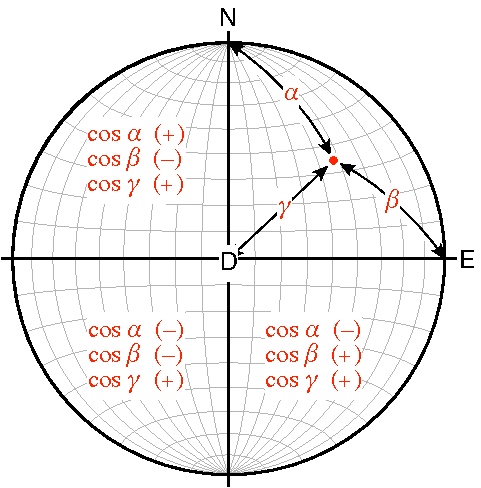
\includegraphics[width=7cm]{ch4f5.pdf}
    \caption{Lower hemisphere stereonet showing the sign of the direction cosines in each quadrant. In the NE quadrant, all three direction cosines are positive. Modified from Allmendinger et al. (2012).}
\end{figure}

The function \href{https://github.com/nfcd/compGeo/blob/master/source/functions/sph_to_cart.py}{sph\_to\_cart} converts a line from spherical to Cartesian coordinates. Notice that the \code{trd} and \code{plg} of the line should be entered in radians:

\begin{center}
\begin{lstlisting}[language=Python, frame=single]
import math

def sph_to_cart(trd,plg):
	"""
	sph_to_cart converts line from spherical (trend 
	and plunge) to Cartesian (direction cosines) 
	coordinates
	
	sph_to_cart(trd,plg) returns the north (cn),
	east (ce), and down (cd) direction cosines of 
	a line with trend = trd and plunge = plg
	
	NOTE: Angles should be entered in radians
	
	Python function based on the Matlab function
	SphToCart in Allmendinger et al. (2012)
	"""
	# Compute direction cosines from trend and plunge
	cn = math.cos(trd) * math.cos(plg)
	ce = math.sin(trd) * math.cos(plg)
	cd = math.sin(plg)
	
	return cn, ce, cd
\end{lstlisting}    
\end{center}

\subsection{From Cartesian to spherical coordinates}

Converting from direction cosines (Cartesian coordinates) to trend and plunge (spherical coordinates) is a little less straightforward. The plunge is easy:

\begin{equation}
    plunge = \sin^{-1}(\cos\gamma) \tag{4.13a}
\end{equation}

The trend can be determined as follows:

\begin{equation*}
    \frac{\cos\beta}{\cos\alpha}=\frac{\sin(trend)\cos(plunge)}{\cos(trend)\cos(plunge)}=\tan(trend)
\end{equation*}

or:

\begin{equation}
    trend = \tan^{-1}\left(\frac{\cos\beta}{\cos\alpha}\right) \tag{4.13b}
\end{equation}

The problem is that the trend varies from 0 and 360\degree. For the $\tan^{-1}$ function, there are two possible angles between 0 and 360\degree. Which one should we use? The answer is to use the signs of the direction cosines to determine in which quadrant the trend lies within. By inspection of Figure 4.5, one can see that:

\begin{equation}
    trend = \tan^{-1}\left(\frac{\cos\beta}{\cos\alpha}\right)\,\,if\,\cos\alpha>0 \tag{4.14a}
\end{equation}

\begin{equation}
    trend = 180\degree+\tan^{-1}\left(\frac{\cos\beta}{\cos\alpha}\right)\,\,if\,\cos\alpha<0 \tag{4.14b}
\end{equation}

One should also check for the special case of $\cos\alpha=0$:

\begin{equation}
    trend = 90\degree\,\,if\,(\cos\alpha = 0\,\,and\,\cos(\beta)\geq 0) \tag{4.14c}
\end{equation}

\begin{equation}
    trend = 270\degree\,\,if\,(\cos\alpha = 0\,\,and\,\cos(\beta)< 0) \tag{4.14d}
\end{equation}

The function \href{https://github.com/nfcd/compGeo/blob/master/source/functions/cart_to_sph.py}{cart\_to\_sph} converts a line from Cartesian to spherical coordinates. Notice that the trend and plunge of the line are returned in radians:

\begin{center}
\begin{lstlisting}[language=Python, frame=single]
import math
from zero_twopi import zero_twopi

def cart_to_sph(cn,ce,cd):
	"""
	cart_to_sph converts from Cartesian to spherical coordinates
	
	cart_to_sph(cn,ce,cd) returns the trend (trd)
	and plunge (plg) of a line with north (cn),
	east (ce), and down (cd) direction cosines
	
	NOTE: Trend and plunge are returned in radians
	
	Python function translated from the Matlab function
	CartToSph in Allmendinger et al. (2012)
	"""
	pi = math.pi
	# Plunge 
	plg = math.asin(cd) 
	
	# Trend: If north direction cosine is zero, trend
	# is east or west. Choose which one by the sign of
	# the east direction cosine
	if cn == 0.0:
		if ce < 0.0:
			trd = 3.0/2.0 * pi # trend is west
		else:
			trd = pi/2.0 # trend is east
	else:
		trd = math.atan(ce/cn) 
		if cn < 0.0:
			trd = trd + pi 
		# Make sure trend is between 0 and 2*pi
		trd = zero_twopi(trd)
	
	return trd, plg
\end{lstlisting}    
\end{center}

% SECTION: APPLICATIONS
\section{Applications}

\subsection{Mean vector}\label{MeanVector}

An important problem in geosciences is to determine the average or mean vector that represents a group of lines. These lines can be for example poles to bedding, paleocurrent directions, paleomagnetic poles, or slip vectors on a fault surface. This problem can be solved using vector addition. The resultant vector $\mathbf{r}$ of the sum of the $N$ unit vectors representing the lines has components:

\begin{equation}
    r_1=\sum_{i=1}^{N}\alpha_i\qquad r_2=\sum_{i=1}^{N}\beta_i\qquad r_3=\sum_{i=1}^{N}\gamma_i \tag{4.15a}
\end{equation}

where $\alpha$, $\beta$ and $\gamma$ are the direction cosines of the unit vectors. The length of the resultant vector $\mathbf{r}$ is:

\begin{equation}
    r=\sqrt{r_1^2+r_2^2+r_3^2} \tag{4.15b}
\end{equation}

and the direction cosines of the unit vector that is parallel to the mean of the individual vectors are:

\begin{equation}
    \overline{\alpha}=\frac{r_1}{r}\qquad \overline{\beta}=\frac{r_2}{r}\qquad \overline{\gamma}=\frac{r_3}{r} \tag{4.15c}
\end{equation}

These direction cosines define the orientation of the mean vector. The mean resultant length $\overline{r}$ measures how concentrated the individual vectors are or how representative the mean vector is:

\begin{equation}
    \overline{r}=\frac{r}{N}\qquad where\qquad 0\leq\overline{r}\leq 1 \tag{4.15d}
\end{equation}

The closer this value is to 1, the better the concentration. The function \href{https://github.com/nfcd/compGeo/blob/master/source/functions/calc_mv.py}{calc\_mv} calculates the mean vector for a series of lines. It also calculates the Fisher statistics for the mean vector (Fisher et al., 1987), which is the standard way to represent uncertainties in this analysis. Notice that \code{calc\_mv} uses our two previous functions \code{sph\_to\_cart} and \code{cart\_to\_sph} to convert from spherical to Cartesian coordinates, and vice versa.

\begin{center}
\begin{lstlisting}[language=Python, frame=single]
import math
from sph_to_cart import sph_to_cart
from cart_to_sph import cart_to_sph

def calc_mv(T,P):
	"""
	calc_mv calculates the mean vector for a group of lines.
	It calculates the trend (trd) and plunge (plg) of the
	mean vector, its mean resultant length (rave), and
	Fisher statistics (concentration factor (conc), 99 (d99)
	and 95 (d95) % uncertainty cones); for a series of lines
	whose trends and plunges are stored in the arrays T and P
	
	NOTE: Input/Output values are in radians
	
	Python function translated from the Matlab function
	CalcMV in Allmendinger et al. (2012)
	"""
	# Number of lines
	nlines = len(T)
	
	# Initialize the 3 direction cosines which contain the
	# sums of the individual vectors 
	cn_sum = ce_sum = cd_sum = 0.0
	
	#Now add up all the individual vectors
	for i in range(nlines):
		cn,ce,cd = sph_to_cart(T[i],P[i])
		cn_sum += cn
		ce_sum += ce
		cd_sum += cd
	
	# r is the length of the resultant vector and
	# rave is the mean resultant length
	r = math.sqrt(cn_sum*cn_sum+ce_sum*ce_sum+cd_sum*cd_sum)
	rave = r/nlines
	# If rave is lower than 0.1, the mean vector is
	# insignificant, return error
	if rave < 0.1:
		raise ValueError("Mean vector is insignificant")
	#Else 
	else:
		# Divide the resultant vector by its length to get
		# the direction cosines of the unit vector
		cn_sum /= r
		ce_sum /= r
		cd_sum /= r
		# Convert the mean vector to the lower hemisphere
		if cd_sum < 0.0:
			cn_sum *= -1.0
			ce_sum *= -1.0
			cd_sum *= -1.0
		# Convert the mean vector to trend and plunge
		trd, plg = cart_to_sph(cn_sum,ce_sum,cd_sum)
		# If there are enough measurements calculate the
		# Fisher statistics (Fisher et al., 1987)
		conc = d99 = d95 = 0.0
		if r < nlines:
			if nlines < 16:
				afact = 1.0-(1.0/nlines)
				conc = (nlines/(nlines-r))*afact**2
			else:
				conc = (nlines-1.0)/(nlines-r)
		if rave >= 0.65 and rave < 1.0:
			afact = 1.0/0.01
			bfact = 1.0/(nlines-1.0)
			d99 = math.acos(1.0-((nlines-r)/r)*(afact**bfact-1.0))
			afact = 1.0/0.05
			d95 = math.acos(1.0-((nlines-r)/r)*(afact**bfact-1.0))
	
	return trd, plg, rave, conc, d99, d95
\end{lstlisting}    
\end{center}

The notebook \href{https://github.com/nfcd/compGeo/blob/master/source/notebooks/ch4-3.ipynb}{ch4-3} solves the mean vector problem in Ragan (2009, pp. 147), which involves finding the mean orientation of 10 poles to bedding:

\begin{center}
\begin{lstlisting}[language=Python, frame=single]
# Import libraries
import numpy as np
import matplotlib.pyplot as plt

# Import functions st_coord_line and calc_mv
import sys, os
sys.path.append(os.path.abspath("../functions"))
from st_coord_line import st_coord_line
from calc_mv import calc_mv

# Arrays T and P contain the trend (T) 
# and plunge (P) of the 10 poles
T = np.radians([206, 220, 204, 198, 200, 188, 192, 
                228, 236, 218])
P = np.radians([32, 30, 46, 40, 20, 32, 54, 56, 36, 44])

# Compute the mean vector and print orientation
# and mean resultant length
trd, plg, rave, conc, d99, d95 = calc_mv(T,P)
pi = np.pi
print("Mean vector trend = {:.1f}, plunge {:.1f}"
      .format(trd*180/pi,plg*180/pi))
print("Mean resultant length = {:.3f}".format(rave))

# Make a figure
fig, ax = plt.subplots()

# Plot the primitive of the stereonet
r = 1; # unit radius
th = np.radians(np.arange(0,361,1))
x = r * np.cos(th)
y = r * np.sin(th)
ax.plot(x,y,"k")
# Plot center of circle
ax.plot(0,0,"k+")
# Make axes equal and remove them
ax.axis("equal")
ax.axis("off")

# Plot the poles as black points
# on an equal angle stereonet
npoles = len(T)
eq_angle = np.zeros((npoles, 2))
for i in range(npoles):
    # Equal angle coordinates
    eq_angle[i,0], eq_angle[i,1] = st_coord_line(T[i],P[i],0)

ax.plot(eq_angle[:,0],eq_angle[:,1],"ko")

# Plot the mean vector as a red point
mvx, mvy = st_coord_line(trd,plg,0)
ax.plot(mvx,mvy,"ro");
\end{lstlisting}
\fbox{
\parbox{\textwidth - 2 \fboxsep}{
Mean vector trend = 208.6, plunge 40.0 \\
Mean resultant length = 0.963 \\
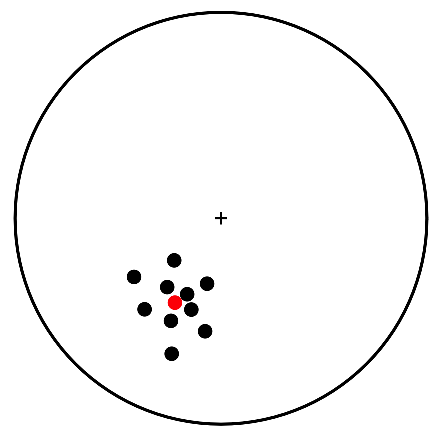
\includegraphics[width=4.25cm]{ch4f6.pdf}
}}
\end{center}

Notice that the mean resultant length is close to 1.0, so that the mean vector (red dot) is a representative orientation of the individual vectors (black dots).

\subsection{Angles, intersections, and poles}

Many interesting problems can be solved using the dot and cross product operations. The dot product can be used to find the angle between two lines or planes, while the cross product can be used to find a plane from two lines, or the intersection of two planes. Table 4.2 lists some problems that can be solved using these operations.

\begin{table}[H]
\small
\centering
\begin{tabular}{ | p{6cm} | p{6cm} | } 
 \hline
 \multicolumn{1}{|c|}{Problem} & \multicolumn{1}{|c|}{Solution}  \\
 \hline
 Angle between two lines & $\arccos$ of dot product between lines \\
 \hline
 Angle between two planes & supplement of $\arccos$ of dot product between poles to planes \\
 \hline
 Intersection of two planes & Cross product of poles to planes \\
 \hline
 Plane containing two lines & Pole to plane is cross product of lines \\
 \hline
 Apparent dip of plane & Intersection of plane and vertical section of a given orientation \\
 \hline
 Plane from two apparent dips & Plane containing the two apparent dips (lines) \\
 \hline
\end{tabular}
\caption{Some problems that can be solved using the dot and cross product operations.}
\label{table4.2}
\end{table}

The functions in the module \href{https://github.com/nfcd/compGeo/blob/master/source/functions/angles.py}{angles} compute the angle between two lines (\code{angle\_bw\_lines}), the angle between two planes (\code{angle\_bw\_planes}), the plane from two lines (\code{plane\_from\_app\_dips}), or the intersection of two planes (\code{int\_bw\_planes}).

\begin{center}
\begin{lstlisting}[language=Python, frame=single]
import numpy as np
from sph_to_cart import sph_to_cart
from cart_to_sph import cart_to_sph
from pole import pole_from_plane, plane_from_pole

# Python functions based on the Matlab function
# Angles in Allmendinger et al. (2012)

def angle_bw_lines(trd1, plg1, trd2, plg2):
	"""
	angle_bw_lines returns the angle between two lines
	of trend and plunge trd1, plg1, trd2, and plg2
	Input and output angles are in radians
	"""
	# convert lines to directions cosines and numpy arrays
	cn1, ce1, cd1 = sph_to_cart(trd1, plg1)
	u = np.array([cn1, ce1, cd1])
	cn2, ce2, cd2 = sph_to_cart(trd2, plg2)
	v = np.array([cn2, ce2, cd2])
	# angle between lines is arccosine of their dot product
	return np.arccos(np.dot(u, v))

def angle_bw_planes(str1, dip1, str2, dip2):
	"""
	angle_bw_planes returns the angle between two planes
	of strike and dip str1, dip1, str2, and dip2
	Input and output angles are in radians
	"""
	# compute poles to lines
	pole1_trd, pole1_plg = pole_from_plane(str1, dip1)
	pole2_trd, pole2_plg = pole_from_plane(str2, dip2)
	# find angle between poles
	angle = angle_bw_lines(pole1_trd, pole1_plg, 
		pole2_trd, pole2_plg)
	# angle between planes is the complementary angle
	return (np.pi - angle)

def pole_from_lines(trd1, plg1, trd2, plg2):
	"""
	pole_from_lines compute the pole to a plane given
	two lines on the plane, with trend and plunge trd1, plg1,
	trd2, and plg2
	Input and output angles are in radians
	"""
	# convert lines to direction cosines and numpy arrays
	cn1, ce1, cd1 = sph_to_cart(trd1, plg1)
	u = np.array([cn1, ce1, cd1])
	cn2, ce2, cd2 = sph_to_cart(trd2, plg2)
	v = np.array([cn2, ce2, cd2])
	# normal is cross product between vectors
	pole = np.cross(u, v)
	# make pole a unit vector
	norm = np.linalg.norm(pole)
	pole = pole/norm
	# if pole points upwards, make it point downwards
	if pole[2] < 0:
		pole *= -1.0
	# return trend and plunge of pole
	return cart_to_sph(pole[0], pole[1], pole[2])

def plane_from_app_dips(trd1, plg1, trd2, plg2):
	"""
	plane_from_app_dips returns the strike and dip of a plane
	from two apparent dips with trend and plunge trd1, plg1,
	trd2, and plg2
	Input and output angles are in radians
	"""
	# Compute pole to plane from apparent dips (lines)
	pole_trd, pole_plg = pole_from_lines(trd1,plg1,trd2,plg2)
	# return strike and dip of plane
	return plane_from_pole(pole_trd, pole_plg)

def int_bw_planes(str1, dip1, str2, dip2):
	"""
	int_bw_planes returns the intersection between two planes
	of strike and dip str1, dip1, str2, dip2
	Input and output angles are in radians
	"""
	# compute poles to planes
	pole1_trd, pole1_plg = pole_from_plane(str1, dip1)
	pole2_trd, pole2_plg = pole_from_plane(str2, dip2)
	# intersection is normal to poles
	return pole_from_lines(pole1_trd, pole1_plg, pole2_trd, 
		pole2_plg)
\end{lstlisting}    
\end{center}

The notebook \href{https://github.com/nfcd/compGeo/blob/master/source/notebooks/ch4-4.ipynb}{ch4-4} illustrates the use of these functions to solve several problems. Let's start with the following problem from Leyshon and Lisle (1996): Two limbs of a chevron fold (A and B) have orientations (RHR) as follows: Limb A = 120/40, Limb B = 250/60. Determine: (a) the trend and plunge of the hinge line of the fold, (b) the rake of the hinge line in limb A, (c) the rake of the hinge line in limb B. 

\begin{center}
\begin{lstlisting}[language=Python, frame=single]
import numpy as np
pi = np.pi

# Import functions 
import sys, os
sys.path.append(os.path.abspath("../functions"))
from angles import angle_bw_lines
from angles import int_bw_planes

# Strike and dip of the limbs in radians
str1, dip1 = np.radians([120, 40])
str2, dip2 = np.radians([250, 60])

# (a) Chevron folds have planar limbs. The hinge
# of the fold is the intersection of the limbs
htrd, hplg = int_bw_planes(str1,dip1,str2,dip2)
print("Hinge trend = {:.1f}, plunge {:.1f}"
      .format(htrd*180/pi,hplg*180/pi))

# The rake of the hinge on either limb is the angle 
# between the hinge and the strike line on the limb. 
# This line is horizontal and has plunge = 0
plg = 0

# (b) For the SW dipping limb
ang = angle_bw_lines(str1,plg,htrd,hplg)
print("Rake of hinge in SW dipping limb = {:.1f} E"
      .format(ang*180/pi))

# (c) And for the NW dipping limb
ang = angle_bw_lines(str2,plg,htrd,hplg)
print("Rake of hinge in NW dipping limb = {:.1f} W"
      .format(ang*180/pi))
\end{lstlisting}
\fbox{
\parbox{\textwidth - 2 \fboxsep}{
Hinge trend = 265.8, plunge 25.3 \\
Rake of hinge in SW dipping limb = 138.4 E \\
Rake of hinge in NW dipping limb = 29.5 W
}}
\end{center}

Let's do another problem from the same book: A quarry has two walls, one trending 002\degree\space and the other 135\degree. The apparent dip of bedding on the faces are 40\degree\space N and 30\degree\space SE respectively. Calculate the strike and dip of bedding.

\begin{center}
\begin{lstlisting}[language=Python, frame=single]
# Import function
from angles import plane_from_app_dips

# The apparent dips are just two lines on bedding
# These lines have orientations:
trd1, plg1 = np.radians([2, 40])
trd2, plg2 = np.radians([135, 30])

# Calculate bedding from these two apparent dips
strike, dip = plane_from_app_dips(trd1,plg1,trd2,plg2)
print("Bedding strike = {:.1f}, dip {:.1f}"
      .format(strike*180/pi,dip*180/pi))
\end{lstlisting}
\fbox{
\parbox{\textwidth - 2 \fboxsep}{
Bedding strike = 333.9, dip 60.7
}}
\end{center}

And the final problem also from the same book: Slickenside lineations trending 074\degree\space occur on a fault with orientation 300/50 (RHR). Determine the plunge of these lineations and their rake in the plane of the fault.

\begin{center}
\begin{lstlisting}[language=Python, frame=single]
# The lineation on the fault is just the intersection
# of a vertical plane with a strike equal to
# the trend of the lineation, and the fault
str1, dip1 = np.radians([74, 90])
str2, dip2 = np.radians([300, 50])

# Find the intersection of these two planes which is
# the lineation on the fault
ltrd, lplg = int_bw_planes(str1,dip1,str2,dip2)
print("Slickensides trend = {:.1f}, plunge {:.1f}"
      .format(ltrd*180/pi,lplg*180/pi))

# And the rake of this lineation is the angle
# between the lineation and the strike line on the fault
plg = 0
ang = angle_bw_lines(str2,plg,ltrd,lplg)
print("Rake of slickensides = {:.1f} W".format(ang*180/pi))
\end{lstlisting}
\fbox{
\parbox{\textwidth - 2 \fboxsep}{
Slickensides trend = 74.0, plunge 40.6 \\
Rake of slickensides = 121.8 W
}}
\end{center}

There are many interesting problems you can solve using these functions. You will find more problems in section \ref{exercises4}.

\subsection{Three points problem}\label{ThreePointProblem}

The three points problem is a fundamental problem in geology. It is based on the fact that three non-collinear points on a plane define the orientation of the plane. The graphical solution to this problem is introduced early in Geosciences. It involves finding the strike line (a line connecting two points of equal elevation) on the plane, and the dip from two strike lines (two structure contours) on the plane. 

However, there is an easier and more accurate solution to this problem using linear algebra: The three points on the plane define two lines, and the cross product between these lines is parallel to the pole to the plane, from which the orientation of the plane can be estimated. The function \href{https://github.com/nfcd/compGeo/blob/master/source/functions/three_points.py}{three\_points} computes the strike and dip of a plane from the east (\textbf{E}), north (\textbf{N}), and up (\textbf{U}) coordinates of three points on the plane:

\begin{center}
\begin{lstlisting}[language=Python, frame=single]
import numpy as np
from cart_to_sph import cart_to_sph
from pole import plane_from_pole

def three_points(p1,p2,p3):
	"""
	three_points calculates the strike (strike) and dip (dip)
	of a plane given the east (E), north (N), and up (U)
	coordinates of three non-collinear points on the plane
	
	p1, p2 and p3 are 1 x 3 arrays defining the location
	of the points in an ENU coordinate system. For each one
	of these arrays the first, second and third entries are 
	the E, N and U coordinates, respectively
	
	NOTE: strike and dip are returned in radians and they
	follow the right-hand rule format
	"""
	# make vectors v (p1 - p3) and u (p2 - p3)
	v = p1 - p2
	u = p2 - p3
	# take the cross product of v and u
	vcu = np.cross(v,u)
	
	# make this vector a unit vector
	mvcu = np.linalg.norm(vcu) # magnitude of the vector
	if mvcu == 0: # If points collinear
		raise ValueError("Error: points are collinear")
	
	vcu = vcu/mvcu # unit vector
	
	# make the pole vector in NED coordinates
	p = np.array([vcu[1], vcu[0], -vcu[2]])
	
	# Make pole point downwards
	if p[2] < 0:
		p *= -1.0
	
	# find the trend and plunge of the pole
	trd, plg = cart_to_sph(p[0],p[1],p[2])
	
	# find strike and dip of plane
	strike, dip = plane_from_pole(trd, plg)
	
	return strike, dip
\end{lstlisting}
\end{center}

Let's use this function in the following problem. The geologic map in Fig. 4.6 shows a sequence of sedimentary units dipping south (you can deduce this by the outcrop V in the valley). Points 1, 2 and 3 are located on the base of unit S and their \textbf{ENU} coordinates are: 

point1 = [509, 2041, 400]

point2 = [1323, 2362, 500]

point3 = [2003, 2913, 700] 

Calculate the strike and dip of the plane. The notebook \href{https://github.com/nfcd/compGeo/blob/master/source/notebooks/ch4-5.ipynb}{ch4-5} shows the solution to this problem:\\ 

\begin{figure}[ht]
    \centering
    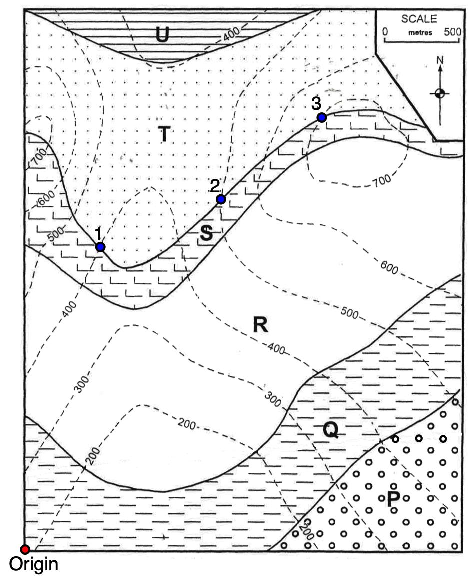
\includegraphics[width=9cm]{ch4f7.pdf}
    \caption{Geologic map of sedimentary units dipping south (Bennison et al., 2011). Points 1 to 3 on the base of unit S are used to estimate the orientation of bedding. Notice that the origin is at the map lower left corner.}
\end{figure}

\begin{center}
\begin{lstlisting}[language=Python, frame=single]
import numpy as np
pi = np.pi

# Import function three_points
import sys, os
sys.path.append(os.path.abspath("../functions"))
from three_points import three_points

# ENU coordinates of the three points
p1 = np.array([509, 2041, 400])
p2 = np.array([1323, 2362, 500])
p3 = np.array([2003, 2913, 700])

# Compute the orientation of the plane
strike, dip = three_points(p1,p2,p3)
print("Plane strike = {:.1f}, dip = {:.1f}"
      .format(strike*180/pi,dip*180/pi))
\end{lstlisting}
\fbox{
\parbox{\textwidth - 2 \fboxsep}{
Plane strike = 84.5, dip = 22.5
}}
\end{center}

% SECTION: Uncertainties
\section{Uncertainties}\label{calcuncertainties}

As we saw in section \ref{uncertainties}, the strike and dip or trend and plunge measurements have errors (Figs. 3.6 and 3.7), and these errors  propagate in any computation making use of these angles. Also, as accurate as GPS and elevation measurements are today, they also have errors. Thus, the functions in the module \code{angles} and the function \code{three\_points} lack this important element of uncertainty.

Suppose that $x, ..., z$ are measured with uncertainties (or errors) $\delta x, ..., \delta z$ and the measured values are used to compute the function $q(x,...,z)$. If the uncertainties in $x, ..., z$ are independent and random, then the uncertainty (or error) in $q$ is (Taylor, 1997):

\begin{equation}
    \delta q=\sqrt{\left(\frac{\partial q}{\partial x}\delta x \right)^2+...+\left(\frac{\partial q}{\partial z}\delta z \right)^2}\tag{4.16}
\end{equation}

This formula is easy to calculate for a few operations, but it can become quite difficult for a long chain of operations. Fortunately, there is a Python package that handles calculations with numbers with uncertainties. This package is called \code{uncertainties} and it was developed by Eric Lebigot. You can find details about the package as well as instructions for installing it in the \href{https://pythonhosted.org/uncertainties/}{uncertainties} website. You can install the uncertainties package by entering in a terminal:

\begin{center}
\begin{lstlisting}[language=Python, frame=single]
pip install --upgrade uncertainties
\end{lstlisting}
\end{center}

After this, you can use the uncertainties package. The module \href{https://github.com/nfcd/compGeo/blob/master/source/functions/angles_u.py}{angles\_u} and the function  \href{https://github.com/nfcd/compGeo/blob/master/source/functions/three_points_u.py}{three\_points\_u} in the resource git repository, are the corresponding \code{angles} module and \code{three\_points} function with uncertainties. We don't list these here, but rather illustrate their use in the following notebook \href{https://github.com/nfcd/compGeo/blob/master/source/notebooks/ch4-6.ipynb}{ch4-6}.

In the first problem on page 64, the uncertainty in strike is 4\degree\space and in dip is 2\degree. What is the uncertainty in the hinge orientation and its rake on the limbs? This problem can be solved as follows:

\begin{center}
\begin{lstlisting}[language=Python, frame=single]
# Import libraries
import numpy as np
pi = np.pi
from uncertainties import ufloat

# Import functions
import sys, os
sys.path.append(os.path.abspath("../functions"))
from angles_u import angle_bw_lines_u
from angles_u import int_bw_planes_u

# Strike and dip of the limbs in radians
str1, dip1 = np.radians([120, 40]) # SW dipping limb
str2, dip2 = np.radians([250, 60]) # NW dipping limb

# Errors in strike and dip in radians
ustr, udip = np.radians([4, 2])

# Create the input values with uncertainties
str1 = ufloat(str1, ustr)  # str1 = str1 +/-ustr
dip1 = ufloat(dip1, udip)  # dip1 = dip1 +/-udip
str2 = ufloat(str2, ustr)  # str2 = str2 +/-ustr
dip2 = ufloat(dip2, udip)  # dip2 = dip2 +/-udip

# (a) Chevron folds have planar limbs. The hinge
# of the fold is the intersection of the limbs
htrd, hplg = int_bw_planes_u(str1,dip1,str2,dip2)
print("Hinge trend = {:.1f}, plunge {:.1f}"
      .format(htrd*180/pi,hplg*180/pi))

# The rake of the hinge on either limb is the angle 
# between the hinge and the strike line on the limb. 
# This line is horizontal and has plunge = 0
plg = ufloat(0, udip)  # plg = 0 +/-udip

# (b) For the SW dipping limb
ang = angle_bw_lines_u(str1,plg,htrd,hplg)
print("Rake of hinge in SW dipping limb = {:.1f} E"
      .format(ang*180/pi))

# (c) And for the NW dipping limb
ang = angle_bw_lines_u(str2,plg,htrd,hplg)
print("Rake of hinge in NW dipping limb = {:.1f} W"
      .format(ang*180/pi))
\end{lstlisting}
\fbox{
\parbox{\textwidth - 2 \fboxsep}{
Hinge trend = 265.8+/-3.3, plunge 25.3+/-2.6 \\
Rake of hinge in SW dipping limb = 138.4+/-4.6 E \\
Rake of hinge in NW dipping limb = 29.5+/-3.5 W
}}
\end{center}

In the map of Fig. 4.6, the error in east and north coordinates is 10 m, and in elevation is 5 m. What is uncertainty in the strike and dip of the T-S contact?

\begin{center}
\begin{lstlisting}[language=Python, frame=single]
# Import function three_points_u
from three_points_u import three_points_u

# ENU coordinates of the three points
# with uncertainties in E-N = 10, and U = 5
p1 = np.array([ufloat(509, 10), ufloat(2041, 10), 
               ufloat(400, 5)])
p2 = np.array([ufloat(1323, 10), ufloat(2362, 10), 
               ufloat(500, 5)])
p3 = np.array([ufloat(2003, 10), ufloat(2913, 10), 
               ufloat(700, 5)])

# Compute the orientation of the plane
strike, dip = three_points_u(p1,p2,p3)
print("Plane strike = {:.1f}, dip = {:.1f}"
      .format(strike*180/pi,dip*180/pi))
\end{lstlisting}
\fbox{
\parbox{\textwidth - 2 \fboxsep}{
Plane strike = 84.5+/-3.5, dip = 22.5+/-2.7
}}
\end{center}

% SECTION: EXERCISES
\section{Exercises} \label{exercises4}

Problems 1-3 are from Marshak and Mitra (1988). Solve these problems using the module \code{angles}.

\begin{enumerate}
    
    \item A fault surface has an orientation (RHR) 190/80. Slickenlines on the fault trend 300\degree. 
    \begin{enumerate}
        \item What is the plunge of the lineation?
        \item What is the rake of the lineation on the fault?
    \end{enumerate}
    
    \item A shale bed has an orientation (RHR) 115/42. What is the apparent dip of the bed in the direction 265\degree?
    
    \item A sandstone bed strikes 140\degree\space across a stream. The stream flows down a narrow gorge with vertical walls. The apparent dip of the bed on the walls of the gorge is 095/25. What is the true dip of the bed?
    
    \item In the geologic map of Fig. 4.7, points 1 to 9 have the following \textbf{ENU} coordinates:
    
    point1 = [1580, 379, 400]
    
    point2 = [1234, 992, 300]
    
    point3 = [2054, 1753, 400]
    
    point4 = [448, 1424, 600]
    
    point5 = [1921, 2195, 500]
    
    point6 = [1408, 3737, 300]
    
    point7 = [536, 2196, 700]
    
    point8 = [743, 2963, 600]
    
    point9 = [2720, 2963, 600]
    
    \begin{enumerate}
        \item Compute the strike and dip of the coal seam (points 1-3).
        \item Compute the strike and dip of the contact where the blue points 4-6 are located. What kind of contact is this? Is the coal seam below or above this contact?
        \item Compute the strike and dip of the contact between units Y and Z (points 7-9). Is this contact below or above the contact in b?
        \item The line of section V-W has a trend of 142\degree. What is the apparent dip of the three contacts above along the section?
        \item Draw a schematic cross section along line V-W
    \end{enumerate}
    
    \textit{Hint}: Use function \code{three\_points} to solve a, b and c. Use the module \code{angles} to solve d.
    
    \begin{figure}[ht]
    \centering
    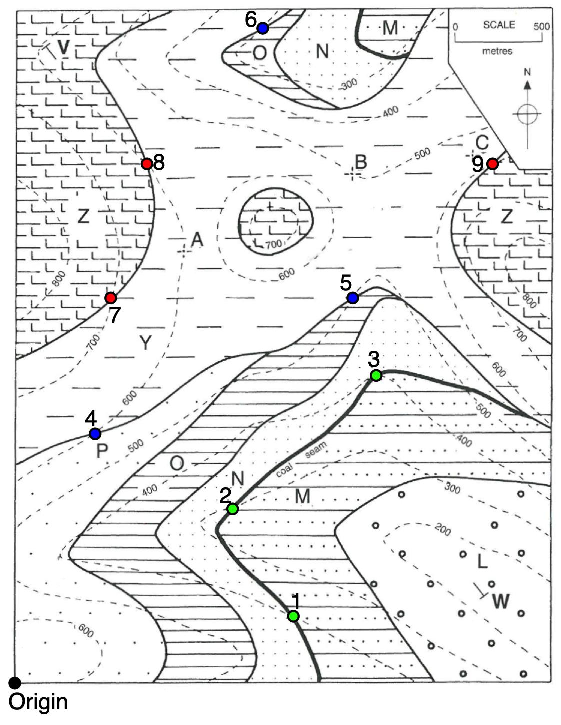
\includegraphics[width=9cm]{ch4f8.pdf}
    \caption{Map for exercise 4. This is map 10 of Bennison et al. (2011).}
    \end{figure}
    
    \item The map of Fig. 4.8 shows an area of a reconnaissance survey in the Appalachian Valley and Ridge Province of western Maryland, USA. On the western half of the map, the contact between a shale horizon (B) and a sandstone unit (C) has been located in two areas. Three points on this contact have the following \textbf{ENU} coordinates:
    
    point1 = [862, 943, 500]
    
    point2 = [692, 1212, 600]
    
    point3 = [1050, 2205, 600]
    
    \begin{figure}[ht]
    \centering
    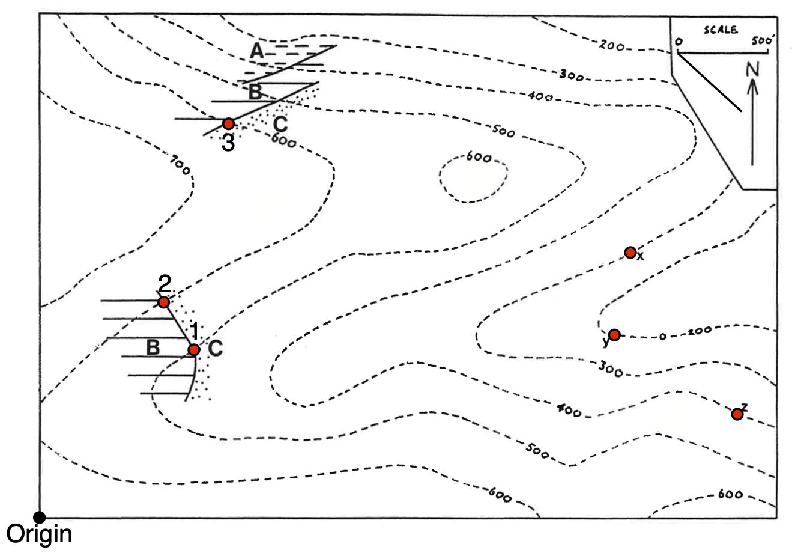
\includegraphics[width=12cm]{ch4f9.pdf}
    \caption{Map for exercise 5}
    \end{figure}
    
    On the eastern half of the map, the contact between B and C was found exposed at three locations labelled x, y, and z. The \textbf{ENU} coordinates of these points are:
    
    pointx = [3298, 1487, 300]
    
    pointy = [3203, 1031, 200]
    
    pointz = [3894, 590, 400]
    
    \begin{enumerate}
        \item Compute the strike and dip of the contact on the western half of the map.
        \item Compute the strike and dip of the contact on the eastern half of the map.
        \item What kind of structure is present on the map? 
        \item Compute the intersection of the western and eastern contacts. What does this line represent?
    \end{enumerate}
    
     \textit{Hint}: Use function \code{three\_points} to solve a and b. Use the module \code{angles} to solve d.
     
     \item In problem 3, the error in azimuth is 5\degree\space and in apparent dip is 3\degree. What is the uncertainty in the true dip of the bed? \textit{Hint}: Use the module \code{angles\_u}.
     
     \item In the map of Fig. 4.7, the east and north coordinates of the points have 15 m error, and the elevations have 5 m error. 
     \begin{enumerate}
        \item What is the uncertainty in the strike and dip of the coal seam?
        \item What is the uncertainty in the strike and dip of the unconformity?
        \item What is the angle between the unconformity and the coal seam and what is the uncertainty in this angle?
    \end{enumerate}
    \textit{Hint}: Use function \code{three\_points\_u} to solve a and b, and the module \code{angles\_u} to solve c.

\end{enumerate}

\addcontentsline{toc}{section}{References}
\section*{References}

Allmendinger, R.W., Cardozo, N. and Fisher, D.W. 2012. Structural Geology Algorithms: Vectors and Tensors. Cambridge University Press.

Bennison, G.M., Olver, P.A. and Moseley, K.A. 2011. An Introduction to Geological Structures and Maps, 8th edition. Hodder Education.

Fisher, N.I., Lewis, T. and Embleton, B.J.J. 1987. Statistical analysis of spherical data. Cambridge University Press.

Leyshon, P.R. and Lisle, R.J. 1996. Stereographic Projection Techniques in Structural Geology. Butterworth Heinemann.

Marshak, S. and Mitra, G. 1988. Basic Methods of Structural Geology. Prentice Hall.

Ragan, D.M. 2009. Structural Geology: An Introduction to Geometrical Techniques. Cambridge University Press.

Taylor, J.R. 1997. An Introduction to Error Analysis, 2nd edition. University Science Books.

% CHAPTER 5: 
\chapter{Transformations}

Many problems in geology, like in real life, are simpler when viewed from another perspective. For example, when studying the movement of continents through time because of plate tectonics (Fig. 5.1a), two coordinate systems are required, one in a present-day geographic frame, and another one attached to the continent. Or to analyze a fault (Fig. 5.1b), we need one coordinate system attached to the fault (with one axis parallel to the pole and another to the slickensides), which we may want to relate to the more familiar \textbf{NED} system. A change in coordinate system is called a coordinate transformation and this is an operation that happens everywhere. Computer games, flight simulators, and subsurface interpretation programs rely heavily on coordinate transformations. 

 \begin{figure}[ht]
    \centering
    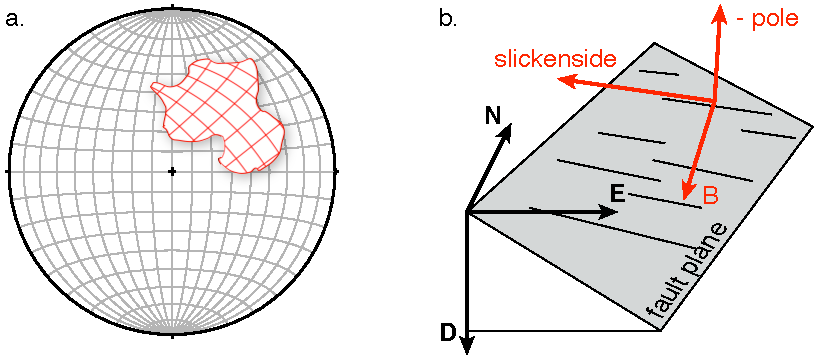
\includegraphics[width=12cm]{ch5f1.pdf}
    \caption{Examples of coordinate transformations in geology. \textbf{a.} Continental drift, \textbf{b.} A fault plane. Red is the local coordinate system for analysis (continent in a, fault in b), and gray/black is the geographic coordinate system. Modified from Allmendinger et al. (2012).}
\end{figure}

\section{Transforming coordinates and vectors}

\subsection{Coordinate transformations}

A transformation involves a change in the origin and orientation of the coordinate system. We will refer to the new axes as the primed coordinate system, $\mathbf{X\text{$'$}}$, and the old coordinate system as the unprimed system, $\mathbf{X}$ (Fig. 5.2a). Let's assume the origin of the old and new coordinate systems is the same. The change in orientation of the new coordinate system is defined by the angles between the new coordinate axes and the old axes. These angles are marked systematically, the first subscript refers to the new coordinate axis and the second subscript to the old coordinate axis. For example, $\theta_{23}$ is the angle between the $\mathbf{X_2\text{$'$}}$ axis and the $\mathbf{X_3}$ axis (Fig. 5.2a). 

 \begin{figure}[ht]
    \centering
    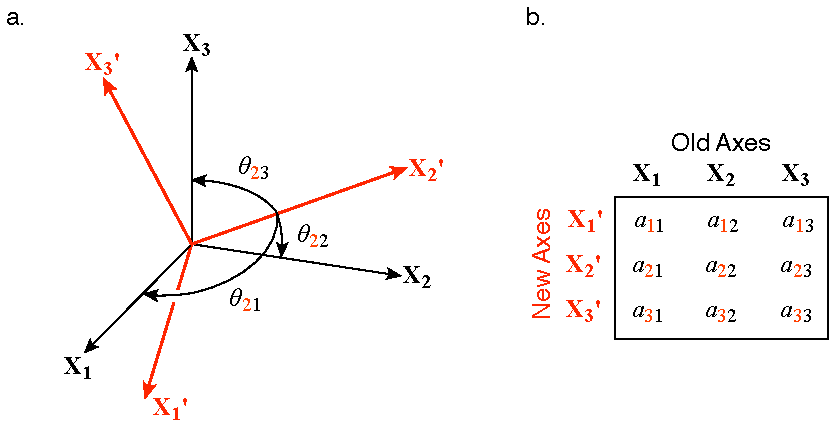
\includegraphics[width=12cm]{ch5f2.pdf}
    \caption{\textbf{a.} Rotation of a Cartesian coordinate system. The old axes are black, the new axes are primed and red. Only three of the nine possible angles are shown. \textbf{b.} Graphic device for remembering how the subscript of the direction cosines relate to the new and the old axes. Modified from Allmendinger et al. (2012).}
\end{figure}

To define the transformation, we use the cosines of these angles rather than the angles themselves (Fig. 5.2b). These are the direction cosines of the new axes with respect to the old axes. The subscript convention is exactly the same. For example, $a_{23}$ is the direction cosine of the $\mathbf{X_2\text{$'$}}$ axis with respect to the $\mathbf{X_3}$ axis. There are nine direction cosines that form a 3 $\times$ 3 array, where each row refers to a new axis and each column to an old axis (Fig. 5.2b). This matrix \textbf{a} of direction cosines is known as the \textit{transformation matrix}, and it is the key element that defines the transformation.

Fortunately, not all the nine direction cosines in the transformation matrix for Fig. 5.2 are independent. Since the base vectors of the new coordinate system are unit vectors, their magnitude is 1:

\begin{equation}
    \begin{gathered}
        a_{11}^2+a_{12}^2+a_{13}^2=1 \\
        a_{21}^2+a_{22}^2+a_{23}^2=1 \\
        a_{31}^2+a_{32}^2+a_{33}^2=1
    \end{gathered}
\end{equation}

and because the base vectors of the new coordinate system are perpendicular to each other, the dot product of two of these axes is zero:

\begin{equation}
    \begin{gathered}
        a_{21}a_{31}+a_{22}a_{32}+a_{23}a_{33}=0 \\
        a_{31}a_{11}+a_{32}a_{12}+a_{33}a_{13}=0 \\
        a_{11}a_{21}+a_{12}a_{22}+a_{13}a_{23}=0
    \end{gathered}
\end{equation}

Equations 5.1 and 5.2 are known as the \textit{orthogonality relations}. Since we have nine unknowns (i.e. the nine direction cosines) and six equations, there are only three independent direction cosines in the transformation matrix. If we know three of the direction cosines defining the transformation, we can calculate the other six.

\subsection{Transformation of vectors}\label{vectortransf}

Once we know the transformation matrix \textbf{a} and the components of a vector in the old coordinate system, we can calculate the components of the vector in the new coordinate system. The equations are fairly simple:

\begin{equation}
    \begin{gathered}
        v_1\text{$'$}=a_{11}v_1+a_{12}v_2+a_{13}v_3 \\
        v_2\text{$'$}=a_{21}v_1+a_{22}v_2+a_{23}v_3 \\
        v_3\text{$'$}=a_{31}v_1+a_{32}v_2+a_{33}v_3
    \end{gathered}
\end{equation}

or using the Einstein summation notation:

\begin{equation}
    v_i\text{$'$}=a_{ij}v_j
\end{equation}

where $i$ is the free suffix, and $j$ is the dummy suffix. Assuming that $i$ and $j$ are either 1, 2, or 3, Equation 5.4 represents three separate equations (the three indices of $i$), each one with three terms (the three indices of $j$). These equations are easy to implement in Python code:

\begin{center}
\begin{lstlisting}[language=Python, frame=single]
for i in range(3):
    v_new[i] = 0
    for j in range(3):
        v_new[i] = a[i,j]*v_old[j] + v_new[i]
\end{lstlisting}
\end{center}

You will see this code snippet repeatedly in the functions of this chapter. Linear algebra is elegant. To convert the vector from the new coordinate system back to the old coordinate system, you just need to do:

\begin{equation}
    v_i=a_{ji}v_j\text{$'$}
\end{equation}

or in Python code:

\begin{center}
\begin{lstlisting}[language=Python, frame=single]
for i in range(3):
    v_old[i] = 0
    for j in range(3):
        v_old[i] = a[j,i]*v_new[j] + v_old[i]
\end{lstlisting}
\end{center}

\subsection{A simple transformation: From \textbf{ENU} to \textbf{NED}}

There is a simple coordinate transformation that nicely illustrates the theory above: the transformation from an \textbf{ENU} to a \textbf{NED} coordinate system (Fig. 4.1). It is simple because the angles involved are either 0, 90, or 180\degree. The direction cosines of the new axes (\textbf{NED}) with respect to the old axes (\textbf{ENU}), and the transformation matrix \textbf{a} is:

\begin{equation}
    \textbf{a}=
    \begin{pmatrix}
    \cos{90} & \cos{0} & \cos{90} \\
    \cos{0} & \cos{90} & \cos{90} \\
    \cos{90} & \cos{90} & \cos{180}
\end{pmatrix}
\end{equation}

which simplifies to:

\begin{equation}\label{eq5.7}
    \textbf{a}=
    \begin{pmatrix}
    0 & 1 & 0 \\
    1 & 0 & 0 \\
    0 & 0 & -1
\end{pmatrix}
\end{equation}

When we use this matrix in Eq. 5.4, we get:

\begin{equation}
    v_1\text{$'$}=v_2;\quad v_2\text{$'$}=v_1; \quad v_3\text{$'$}=-v_3;
\end{equation}

Notice that in this special case \textbf{a} is symmetric ($a_{ij}=a_{ji}$), so the elements of \textbf{a} are also the direction cosines of  \textbf{ENU} with respect to \textbf{NED}. In the following sections, we will look at more complicated coordinate transformations, but the principles mentioned here will still apply.

\section{Applications}

\subsection{Stratigraphic thickness}

The thickness of a tabular stratigraphic unit is the perpendicular distance between the parallel planes bounding the unit. This is also called the stratigraphic thickness (Ragan, 2009). A general problem though is that locations on the planes bounding the unit, are commonly given in a geographic (e.g. \textbf{ENU}) coordinate system. One therefore must use ortographic projections and trigonometry to determine the stratigraphic thickness of the unit from the locations (Ragan, 2009).

An easier approach is to use a transformation. Figure 5.3 illustrates the situation. Points on the top and base of the unit are given in an \textbf{ENU} coordinate system. We can transform these points into a coordinate system attached to the bedding planes, where the strike (RHR) of the planes is the first axis, the dip the second axis, and the pole to the planes the third axis. We will call this coordinate system the \textbf{SDP} system. The thickness of the unit is just the difference between the \textbf{P} coordinates of any point on the top  and any point on the base of the unit.

 \begin{figure}[ht]
    \centering
    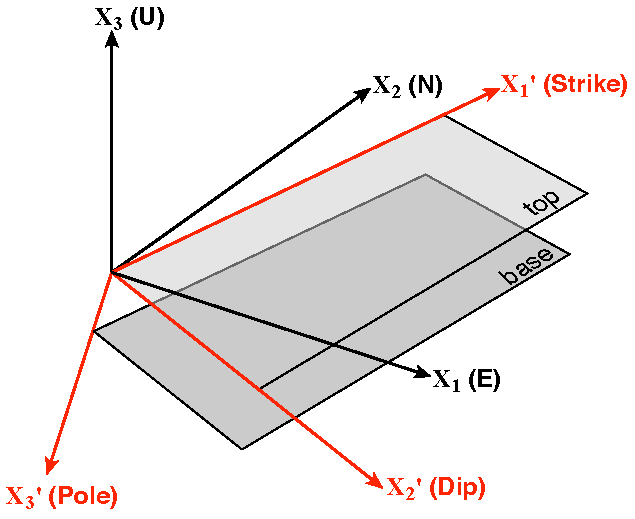
\includegraphics[width=10cm]{ch5f3.pdf}
    \caption{Coordinate transformation from an \textbf{ENU} to a Strike-Dip-Pole (\textbf{SDP}) coordinate system. The thickness of the unit can be calculated by subtracting the \textbf{P} coordinates of any point on the top and any point on the base. Modified from Allmendinger (2020a).}
\end{figure}

We can find the elements of the matrix \textbf{a} for this transformation using trigonometry. However, we will follow a more didactic approach. We will reference the two \textbf{ENU} and \textbf{SDP} coordinate systems with respect to the \textbf{NED} coordinate system, and then use the dot product to determine the direction cosines of \textbf{SDP} into \textbf{ENU}. 

The direction cosines of the \textbf{ENU} coordinate system with respect to the \textbf{NED} coordinate system are given by Eq. \ref{eq5.7}. The direction cosines of the \textbf{SDP} coordinate system with respect to the \textbf{NED} coordinate system can be found using Table \ref{table4.1}:

\begin{gather*}
    \mathbf{S} = [\cos(strike),\sin(strike),0] \\
    \mathbf{D} = [\cos(strike+90)\cos(dip),\sin(strike+90)\cos(dip),\sin(dip)] \\
    \mathbf{P} = [\cos(strike-90)\cos(90-dip),\sin(strike-90)\cos(90-dip),\sin(90-dip)]
\end{gather*}

which simplifies to:

\begin{equation}
    \begin{gathered}
        \mathbf{S} = [\cos(strike),\sin(strike),0]  \\
        \mathbf{D} = [-\sin(strike)\cos(dip),\cos(strike)\cos(dip),\sin(dip)] \\
        \mathbf{P} = [\sin(strike)\sin(dip),-\cos(strike)\sin(dip),\cos(dip)]
    \end{gathered}
\end{equation}

The transformation matrix \textbf{a} from the \textbf{ENU} to the \textbf{SDP} coordinate system has as components the direction cosines of the new \textbf{SDP} axes into the old \textbf{ENU} axes. From Eq. 4.9, one can see that these are just the dot product between the new and old axes:

\begin{equation*}
    \textbf{a}=
    \begin{pmatrix}
    \mathbf{S}\cdot\mathbf{E} & \mathbf{S}\cdot\mathbf{N} & \mathbf{S}\cdot\mathbf{U} \\
    \mathbf{D}\cdot\mathbf{E} & \mathbf{D}\cdot\mathbf{N} & \mathbf{D}\cdot\mathbf{U} \\
    \mathbf{P}\cdot\mathbf{E} & \mathbf{P}\cdot\mathbf{N} & \mathbf{P}\cdot\mathbf{U}
\end{pmatrix}
\end{equation*}

which is equal to:

\begin{equation}
    \textbf{a}=
    \begin{pmatrix}
    \sin(strike) & \cos(strike) & 0 \\
    \cos(strike)\cos(dip) & -\sin(strike)\cos(dip) & -\sin(dip) \\
    -\cos(strike)\sin(dip) & \sin(strike)\sin(dip) & -\cos(dip)
\end{pmatrix}
\end{equation}

So if point 1 is at the top of the unit and has coordinates $[E_1,N_1,U_1]$, and point 2 is at the base of the unit and has coordinates $[E_2,N_2,U_2]$, the \textbf{P} coordinates of these points are:

\begin{equation}
    \begin{gathered}
        P_1 = -\cos(strike)\sin(dip)E_1+\sin(strike)\sin(dip)N_1-\cos(dip)U_1  \\
        P_2 = -\cos(strike)\sin(dip)E_2+\sin(strike)\sin(dip)N_2-\cos(dip)U_2  \\
    \end{gathered}
\end{equation}

and the thickness of the unit is:

\begin{equation}
    t = P_2-P_1
\end{equation}{}

The function \href{https://github.com/nfcd/compGeo/blob/master/source/functions/true_thickness.py}{true\_thickness} calculates the thickness of a unit given the strike and dip of the unit, and the \textbf{ENU} coordinates of two top and base points:

\begin{center}
\begin{lstlisting}[language=Python, frame=single]
import numpy as np

def true_thickness(strike,dip,top,base):
	"""
	true_thickness calculates the thickness (t) of a unit
	given the strike (strike) and dip (dip) of the unit,
	and points at its top (top) and base (base)
	
	top and base are 1 x 3 arrays defining the location
	of top and base points in an ENU coordinate system.
	For each one of these arrays, the first, second
	and third entries are the E, N and U coordinates
	
	NOTE: strike and dip should be input in radians
	"""
	# make the transformation matrix a 
	# from ENU coordinates to SDP coordinates
	sin_str = np.sin(strike)
	cos_str = np.cos(strike)
	sin_dip = np.sin(dip)
	cos_dip = np.cos(dip)
	a = np.array([[sin_str, cos_str, 0],
	[cos_str*cos_dip, -sin_str*cos_dip, -sin_dip],
	[-cos_str*sin_dip, sin_str*sin_dip, -cos_dip]])
	
	# transform the top and base points
	# from ENU to SDP coordinates
	topn = np.zeros(3)
	basen = np.zeros(3)
	for i in range(0,3):
		for j in range(0,3):
			topn[i] = a[i,j]*top[j] + topn[i]
			basen[i] = a[i,j]*base[j] + basen[i]
	
	# compute the thickness of the unit
	t = np.abs(basen[2] - topn[2])
	
	return t
\end{lstlisting}
\end{center}
 
Let's use this function to determine the thickness of the sedimentary units T to Q in the geologic map of Fig. 5.4. This time we have points at the top and base of these units, and their \textbf{ENU} coordinates are:

 \begin{figure}[ht]
    \centering
    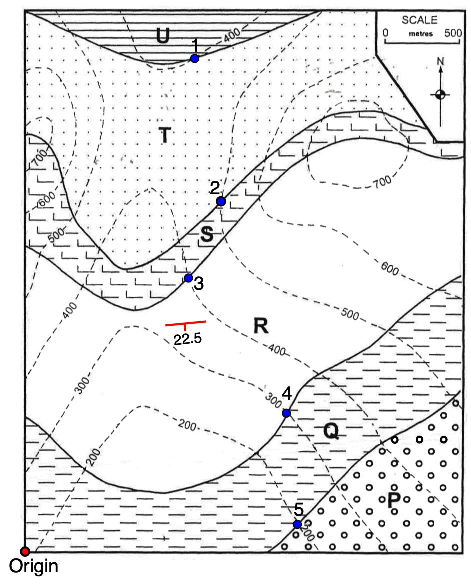
\includegraphics[width=9cm]{ch5f4.pdf}
    \caption{Geologic map of sedimentary units with an orientation 84.5/22.5 (RHR) (Bennison et al.,  2011). Points at the top and base of units T to Q are used to determine the thickness of the units.}
\end{figure}

point1 = [1147, 3329, 400]

point2 = [1323, 2362, 500]

point3 = [1105, 1850, 400]

point4 = [1768, 940, 300]

point5 = [1842, 191, 200]

The notebook \href{https://github.com/nfcd/compGeo/blob/master/source/notebooks/ch5-1.ipynb}{ch5-1} shows the solution to this problem:

\begin{center}
\begin{lstlisting}[language=Python, frame=single]
import numpy as np
pi = np.pi

# Import function true_thickness
import sys, os
sys.path.append(os.path.abspath("../functions"))
from true_thickness import true_thickness

# Strike and dip of the unit in radians
strike, dip = np.radians([84.5, 22.5]) 

# ENU coordinates of the points
p1 = np.array([1147, 3329, 400]) 
p2 = np.array([1323, 2362, 500]) 
p3 = np.array([1105, 1850, 400]) 
p4 = np.array([1768, 940, 300]) 
p5 = np.array([1842, 191, 200])

# Compute the thickness of the units
thickT = true_thickness(strike,dip,p2,p1)
thickS = true_thickness(strike,dip,p3,p2)
thickR = true_thickness(strike,dip,p4,p3)
thickQ = true_thickness(strike,dip,p5,p4)
print("Thickness of unit T = {:.1f} m".format(thickT))
print("Thickness of unit S = {:.1f} m".format(thickS))
print("Thickness of unit R = {:.1f} m".format(thickR))
print("Thickness of unit Q = {:.1f} m".format(thickQ))
\end{lstlisting}
\fbox{
\parbox{\textwidth - 2 \fboxsep}{
Thickness of unit T = 467.2 m \\
Thickness of unit S = 94.6 m \\
Thickness of unit R = 278.6 m \\
Thickness of unit Q = 195.6 m
}}
\end{center}

What about if there are uncertainties in the strike and dip of the unit, and in the coordinates of the top and base points? The function \href{https://github.com/nfcd/compGeo/blob/master/source/functions/true_thickness_u.py}{true\_thickness\_u} in the resource git repository handles this case. Suppose that in the problem above, the uncertainties in strike and dip are 4\degree\space and 2\degree\space respectively, the uncertainty in east and north coordinates is 10 m, and in elevation is 5 m. The notebook \href{https://github.com/nfcd/compGeo/blob/master/source/notebooks/ch5-2.ipynb}{ch5-2} shows the solution to this problem:

\begin{center}
\begin{lstlisting}[language=Python, frame=single]
# Import libraries
import numpy as np
pi = np.pi
from uncertainties import ufloat

# Import function true_thickness_u
import sys, os
sys.path.append(os.path.abspath("../functions"))
from true_thickness_u import true_thickness_u

# Strike and dip of the unit in radians
strike, dip = np.radians([84.5, 22.5]) 

# Strike and dip errors in radians
ustrike, udip = np.radians([4, 2]) 

# Create the strike and dip with uncertainties
strike = ufloat(strike, ustrike) 
dip = ufloat(dip, udip)

# ENU coordinates of the points
# with uncertainties in E-N = 10, and U = 5
p1 = np.array([ufloat(1147, 10), ufloat(3329, 10), 
               ufloat(400, 5)]) 
p2 = np.array([ufloat(1323, 10), ufloat(2362, 10), 
               ufloat(500, 5)]) 
p3 = np.array([ufloat(1105, 10), ufloat(1850, 10), 
               ufloat(400, 5)]) 
p4 = np.array([ufloat(1768, 10), ufloat(940, 10), 
               ufloat(300, 5)]) 
p5 = np.array([ufloat(1842, 10), ufloat(191, 10), 
               ufloat(200, 5)])

# Compute the thickness of the units
thickT = true_thickness_u(strike, dip, p2, p1)
thickS = true_thickness_u(strike, dip, p3, p2)
thickR = true_thickness_u(strike, dip, p4, p3)
thickQ = true_thickness_u(strike, dip, p5, p4) 
print("Thickness of unit T = {:.1f} m".format(thickT))
print("Thickness of unit S = {:.1f} m".format(thickS))
print("Thickness of unit R = {:.1f} m".format(thickR))
print("Thickness of unit Q = {:.1f} m".format(thickQ))
\end{lstlisting}
\fbox{
\parbox{\textwidth - 2 \fboxsep}{
Thickness of unit T = 467.2+/-31.5 m \\
Thickness of unit S = 94.6+/-20.4 m \\
Thickness of unit R = 278.6+/-37.0 m \\
Thickness of unit Q = 195.6+/-27.0 m
}}
\end{center}

For the thinnest unit S, the uncertainty in thickness is about 20\% the thickness of the unit!

\subsection{Outcrop trace of a plane} \label{outcrop}

The \textbf{ENU} to \textbf{SDP} transformation is useful to solve another interesting problem, namely the outcrop trace of a plane on irregular terrain (Fig. \ref{fig:outrace}; Allmendinger, 2020b). If we know the orientation of the plane (strike and dip), the \textbf{ENU} coordinates of a location where the plane outcrops, and the topography of the terrain as a digital elevation model (DEM\footnote{A grid of regularly spaced points in east and north and with elevation at each point.}), we can determine the outcrop trace of the plane using computation. The solution is surprisingly simple, the plane outcrops wherever the \textbf{P} coordinate of the terrain is equal to the \textbf{P} coordinate of the plane's outcrop location.

Let's call the \textbf{P} coordinate of the plane's outcrop location $P_1$, and the \textbf{P} coordinate of a point in the DEM grid $P_{gp}$. The difference between these two is:

\begin{equation}
    D=P_1-P_{gp}
\end{equation}

At each point in the DEM grid, we can calculate and store this difference. The plane will outcrop wherever $D$ is zero. Therefore, to draw the outcrop trace, we just need to contour the $D$ value of zero on the grid. The function \href{https://github.com/nfcd/compGeo/blob/master/source/functions/outcrop_trace.py}{outcrop\_trace} computes the value of $D$ on a DEM grid of regularly spaced points defined by \textbf{E} ($\mathbf{XG}$), \textbf{N} ($\mathbf{YG}$) and \textbf{U} ($\mathbf{ZG}$) coordinates. Notice that these arrays must follow the format given by the NumPy \code{meshgrid} function:

\begin{center}
\begin{lstlisting}[language=Python, frame=single]
import numpy as np

def outcrop_trace(strike,dip,p1,XG,YG,ZG):
	"""
	outcrop_trace estimates the outcrop trace of a plane,
	given the strike (strike) and dip (dip) of the plane,
	the ENU coordinates of a point (p1) where the plane
	outcrops, and a DEM of the terrain as a regular grid
	of points with E (XG), N (YG) and U (ZG) coordinates.
	
	After using this function, to draw the outcrop trace
	of the plane, you just need to draw the contour 0 on
	the grid XG,YG,DG
	
	NOTE: strike and dip should be input in radians
		p1 must be an array
		XG and YG arrays should be constructed using
		the numpy function meshgrid
	"""
	# make the transformation matrix from ENU coordinates to
	# SDP coordinates. We just need the third row of this
	# matrix
	a = np.zeros((3,3))
	a[2,0] = -np.cos(strike)*np.sin(dip) 
	a[2,1] = np.sin(strike)*np.sin(dip) 
	a[2,2] = -np.cos(dip);
	
	# Initialize DG
	n, m = XG.shape
	DG = np.zeros((n,m))
	
	# Estimate the P coordinate of the outcrop point p1
	P1 = a[2,0]*p1[0] + a[2,1]*p1[1] + a[2,2]*p1[2]
	
	# Estimate the P coordinate at each point of the DEM
	# grid and subtract P1
	for i in range(0,n):
		for j in range(0,m):
			DG[i,j] = P1 - (a[2,0]*XG[i,j] + a[2,1]*YG[i,j] 
				+ a[2,2]*ZG[i,j])
	
	return DG
\end{lstlisting}
\end{center}

Let's apply this function to the map of Fig. 5.5. On the western half of this map, the contact between units B and C outcrops at point 1 and has an orientation 020/22 (RHR). On the eastern half of the map, the same contact outcrops at point 2 and has an orientation 160/22 (RHR). The notebook \href{https://github.com/nfcd/compGeo/blob/master/source/notebooks/ch5-3.ipynb}{ch5-3} draws the outcrop trace of the contact. Notice that the \textbf{ENU} coordinates of the points of the DEM grid are input from the text files \href{https://github.com/nfcd/compGeo/blob/master/source/data/ch5-3/XG.txt}{XG}, \href{https://github.com/nfcd/compGeo/blob/master/source/data/ch5-3/YG.txt}{YG}, and \href{https://github.com/nfcd/compGeo/blob/master/source/data/ch5-3/ZG.txt}{ZG}.

 \begin{figure}[t]
    \centering
    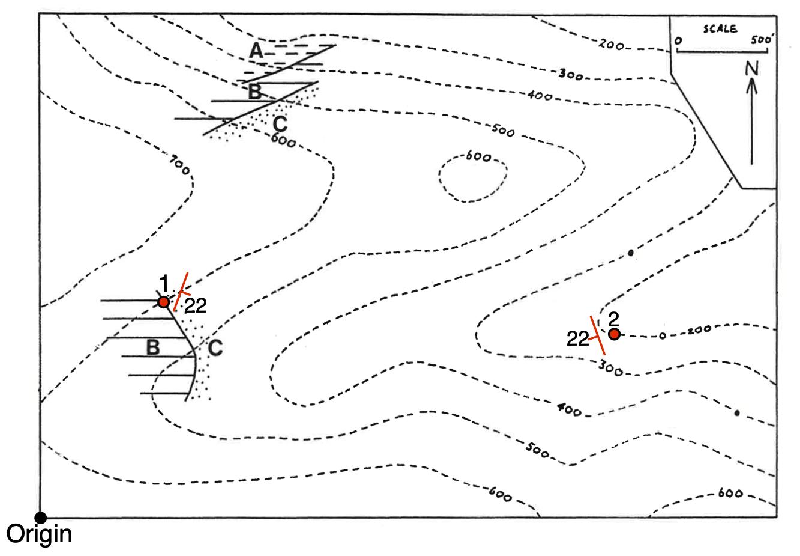
\includegraphics[width=11.8cm]{ch5f5.pdf}
    \caption{The contact between units B and C outcrops at point 1 with orientation 020/22 (RHR), and at point 2 with orientation 160/22 (RHR). From this information and a DEM of the terrain, we can determine the outcrop trace of the contact.}
\end{figure}

\begin{center}
\begin{lstlisting}[language=Python, frame=single]
# Import libraries
import numpy as np
import matplotlib.pyplot as plt

# Import function outcrop_trace
import sys, os
sys.path.append(os.path.abspath("../functions"))
from outcrop_trace import outcrop_trace

# Read the DEM grid
XG = np.loadtxt(os.path.abspath("../data/ch5-3/XG.txt"))
YG = np.loadtxt(os.path.abspath("../data/ch5-3/YG.txt"))
ZG = np.loadtxt(os.path.abspath("../data/ch5-3/ZG.txt"))

# Make a figure
fig, ax = plt.subplots()

# Contour the terrain
cval = np.linspace(200,700,6)
cp = ax.contour(XG,YG,ZG,cval)
ax.clabel(cp, inline=True, fontsize=10, fmt="%d")

# Western contact
pi = np.pi
strike, dip = np.radians([20, 22]) 
point1 = np.array([692, 1212, 600])
DG = outcrop_trace(strike,dip,point1,XG,YG,ZG)
cval = 0 # Contour only CG zero value
cp = ax.contour(XG,YG,DG,cval,colors="red",linewidths=3)
ax.plot(point1[0],point1[1],"bo",markersize=10)

# Eastern contact
strike, dip = np.radians([160, 22]) 
point2 = np.array([3203, 1031, 200])
DG = outcrop_trace(strike,dip,point2,XG,YG,ZG)
cp = ax.contour(XG,YG,DG,cval,colors="red",linewidths=3)
ax.plot(point2[0],point2[1],"bo",markersize=10)

# Make axes equal
ax.axis("equal");
\end{lstlisting}
\fbox{
\parbox{\textwidth - 2 \fboxsep}{
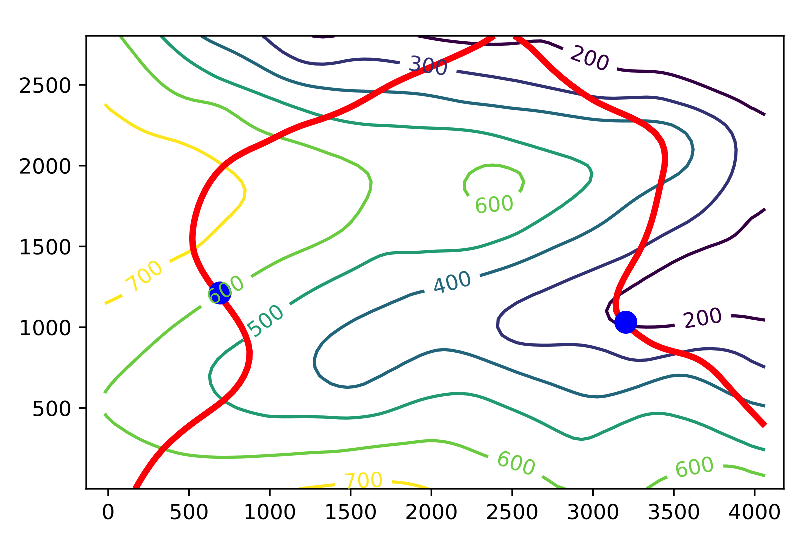
\includegraphics[width=9cm]{ch5f6.pdf}
}}
\end{center}

\subsection{Down-plunge projection}

Folded rock layers normally have a cylindrical symmetry; the layers are bent about a single axis or direction, called the fold axis. In a cylindrical fold, the fold axis is a line of minimum, zero curvature, and the lines of maximum, non-zero curvature are perpendicular to it (Suppe, 1985). The least distorted view of such structure is on the plane perpendicular to the fold axis, which is called the profile plane (Fig. 5.6). Projecting the fold data to this profile plane is called a \textit{down-plunge} projection.

Constructing a down-plunge projection by hand typically involves an orthographic projection, and this problem is complicated (and tedious), particularly if points on the fold are not at the same elevation. Fortunately, we can solve this problem as a coordinate transformation, where points on the fold referenced in a \textbf{ENU} coordinate system, are transformed to a new $\mathbf{X_1\text{$'$}}\mathbf{X_2\text{$'$}}\mathbf{X_3\text{$'$}}$ coordinate system, with $\mathbf{X_3\text{$'$}}$ parallel to the fold axis, and $\mathbf{X_1\text{$'$}}\mathbf{X_2\text{$'$}}$ defining the profile plane (Fig. 5.6).

We will again derive the matrix \textbf{a} for this transformation using linear algebra. The direction cosines of the \textbf{ENU} coordinate system with respect to the \textbf{NED} coordinate system are given by Eq. \ref{eq5.7}. The direction cosines of the $\mathbf{X_1\text{$'$}}\mathbf{X_2\text{$'$}}\mathbf{X_3\text{$'$}}$ coordinate system with respect to the \textbf{NED} coordinate system can be found using Table \ref{table4.1}. If the trend and plunge of the fold axis are $T$ and $P$, these direction cosines are (Fig. 5.6):

\begin{figure}[ht]
    \centering
    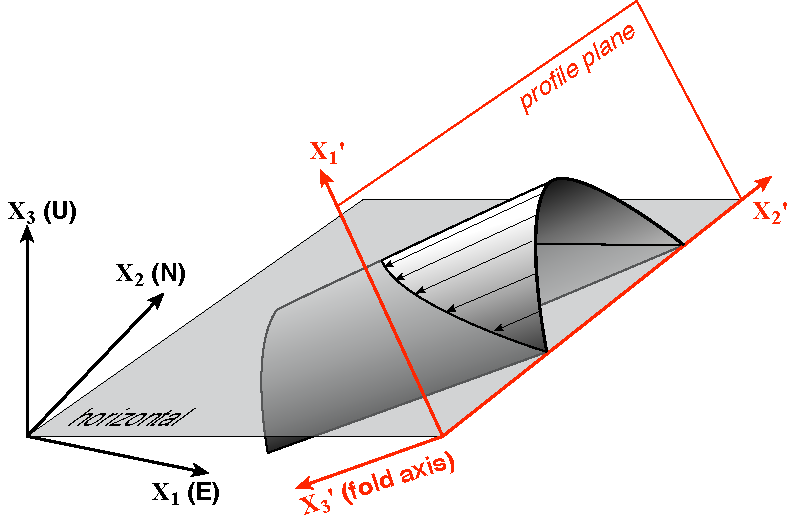
\includegraphics[width=12cm]{ch5f7.pdf}
    \caption{The two coordinate systems involved in a down-plunge projection of a fold. Modified from Allmendinger et al. (2012).}
\end{figure}

\begin{gather*}
    \mathbf{X_1\text{$'$}} = [\cos(T)\cos(P-90),\sin(T)\cos(P-90),\sin(P-90)] \\
    \mathbf{X_2\text{$'$}} = [\cos(T+90),\sin(T+90),0)] \\
    \mathbf{X_3\text{$'$}} = [\cos(T)\cos(P),\sin(T)\cos(P),\sin(P)]
\end{gather*}

which simplifies to:

\begin{equation}
    \begin{gathered}
        \mathbf{X_1\text{$'$}} = [\cos(T)\sin(P),\sin(T)\sin(P),-\cos(P)]  \\
        \mathbf{X_2\text{$'$}} = [-\sin(T),\cos(T),0] \\
        \mathbf{X_3\text{$'$}} = [\cos(T)\cos(P),\sin(T)\cos(P),\sin(P)]
    \end{gathered}
\end{equation}

The direction cosines of the new $\mathbf{X_1\text{$'$}}\mathbf{X_2\text{$'$}}\mathbf{X_3\text{$'$}}$ axes into the old \textbf{ENU} axes are the dot product between the new and old axes:

\begin{equation*}
    \textbf{a}=
    \begin{pmatrix}
    \mathbf{X_1\text{$'$}}\cdot\mathbf{E} & \mathbf{X_1\text{$'$}}\cdot\mathbf{N} & \mathbf{X_1\text{$'$}}\cdot\mathbf{U} \\
    \mathbf{X_2\text{$'$}}\cdot\mathbf{E} & \mathbf{X_2\text{$'$}}\cdot\mathbf{N} & \mathbf{X_2\text{$'$}}\cdot\mathbf{U} \\
    \mathbf{X_3\text{$'$}}\cdot\mathbf{E} & \mathbf{X_3\text{$'$}}\cdot\mathbf{N} & \mathbf{X_3\text{$'$}}\cdot\mathbf{U}
\end{pmatrix}
\end{equation*}

which is equal to:

\begin{equation}
    \textbf{a}=
    \begin{pmatrix}
    \sin(T)\sin(P) & \cos(T)\sin(P) & \cos(P) \\
    \cos(T) & -\sin(T) & 0 \\
    \sin(T)\cos(P) & \cos(T)\cos(P) & -\sin(P)
\end{pmatrix}
\end{equation}

This is the transformation matrix \textbf{a} for the down-plunge projection. To project $i$-th points on the fold with coordinates $[E_i,N_i,U_i]$, we just need to do the following:

\begin{equation}
    \begin{gathered}
        X_{1i}'=\sin(T)\sin(P)E_i+\cos(T)\sin(P)N_i+\cos(P)U_i \\
        X_{2i}'=\cos(T)E_i-\sin(T)N_i
    \end{gathered}
\end{equation}

and then plot $X_{2i}'$ against $X_{1i}'$ (Fig. 5.6) to draw the fold.

The function \href{https://github.com/nfcd/compGeo/blob/master/source/functions/down_plunge.py}{down\_plunge} computes the down-plunge projection of a bed from the \textbf{ENU} coordinates of points on the bed, and the fold axis orientation:

\begin{lstlisting}[language=Python, frame=single]
import numpy as np

def down_plunge(bs,trd,plg):
	"""
	down_plunge constructs the down plunge projection of a bed
	
	bs is a npoints x 3 array, which holds npoints
	on the digitized bed, each point defined by
	3 coordinates: X1 = East, X2 = North, X3 = Up
	
	trd and plg are the trend and plunge of the fold axis
	and they should be entered in radians
	
	dpbs are the bed's transformed coordinates
	
	Python function translated from the Matlab function
	DownPlunge in Allmendinger et al. (2012)
	"""
	# Number of points in bed
	nvtex = bs.shape[0]
	
	# Allocate some arrays
	a=np.zeros((3,3))
	dpbs = np.zeros((np.shape(bs)))
	
	# Calculate the transformation matrix a(i,j)
	a[0,0] = np.sin(trd)*np.sin(plg)
	a[0,1] = np.cos(trd)*np.sin(plg)
	a[0,2] = np.cos(plg)
	a[1,0] = np.cos(trd)
	a[1,1] = -np.sin(trd)
	a[2,0] = np.sin(trd)*np.cos(plg)
	a[2,1] = np.cos(trd)*np.cos(plg)
	a[2,2] = -np.sin(plg)
	
	# Perform transformation
	for nv in range(0,nvtex):
		for i in range(0,3):
			dpbs[nv,i] = 0.0
			for j in range(0,3):
					dpbs[nv,i] = a[i,j]*bs[nv,j] + dpbs[nv,i]
	
	return dpbs
\end{lstlisting}

Let's use this function to draw the down-plunge projection of the Big Elk anticline, southeastern Idaho, USA (Fig. 5.7; Albee and Cullins, 1975). Text files contain the digitized contacts (\textbf{ENU}) of three tops along the fold: the Jurassic Twin Creek Limestone (\href{https://github.com/nfcd/compGeo/blob/master/source/data/ch5-4/jtc.txt}{jtc.txt}), the Jurassic Stump Sandstone (\href{https://github.com/nfcd/compGeo/blob/master/source/data/ch5-4/js.txt}{js.txt}), and the Cretaceous Peterson Limestone (\href{https://github.com/nfcd/compGeo/blob/master/source/data/ch5-4/kp.txt}{kp.txt}). The trend and plunge of the folds axis is 125/26 (in the next chapter we will see how to compute this axis). The notebook \href{https://github.com/nfcd/compGeo/blob/master/source/notebooks/ch5-4.ipynb}{ch5-4} shows the solution to this problem:

\begin{figure}
    \centering
    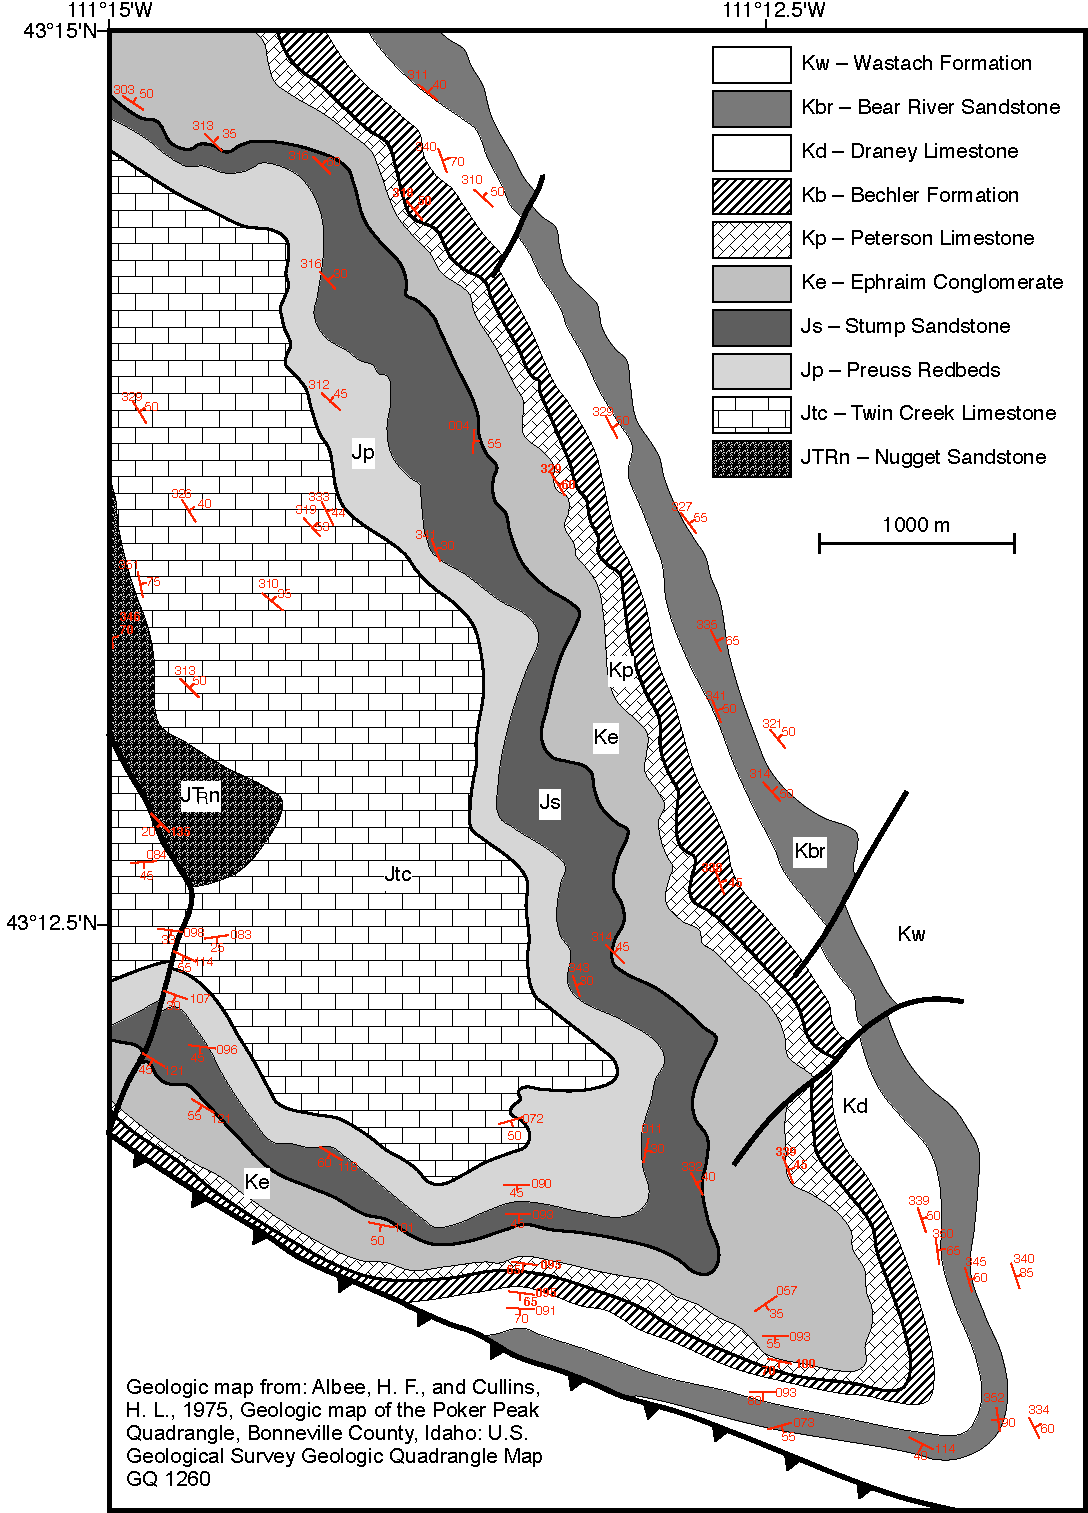
\includegraphics[width=13cm]{ch5f8.pdf}
    \caption{Simplified geologic map of the Big Elk anticline in southeastern Idaho. Modified from Allmendinger et al. (2012).}
    \label{fig:bigElkAnticline}
\end{figure}

\begin{center}
\begin{lstlisting}[language=Python, frame=single]
# Import libraries
import numpy as np
import matplotlib.pyplot as plt

# Import function down_plunge
import sys, os
sys.path.append(os.path.abspath("../functions"))
from down_plunge import down_plunge

# Trend and plunge of the fold axis in radians
trend, plunge = np.radians([125, 26]) 

# Read the tops from the text files
jtc = np.loadtxt(os.path.abspath("../data/ch5-4/jtc.txt"))
js = np.loadtxt(os.path.abspath("../data/ch5-4/js.txt"))
kp = np.loadtxt(os.path.abspath("../data/ch5-4/kp.txt"))

# Transform the points
jtcdp = down_plunge(jtc,trend,plunge)
jsdp = down_plunge (js,trend,plunge)
kpdp = down_plunge(kp,trend,plunge)

# Make a figure
fig, ax = plt.subplots()

# Plot the down plunge section
ax.plot(jtcdp[:,1],jtcdp[:,0],"k-")
ax.plot(jsdp[:,1],jsdp[:,0],"r-")
ax.plot(kpdp[:,1],kpdp[:,0],"b-")

# Display the section"s orientation
# Notice that the fold axis plunges SE
# Therefore the left side of the section is NE
# and the right side is SW
ax.text(-2.1e4,12e3,"NE")
ax.text(-0.6e4,12e3,"SW")

# Make axes equal
ax.axis("equal");
\end{lstlisting}
\end{center}

\begin{center}
\fbox{
\parbox{\textwidth - 2 \fboxsep}{
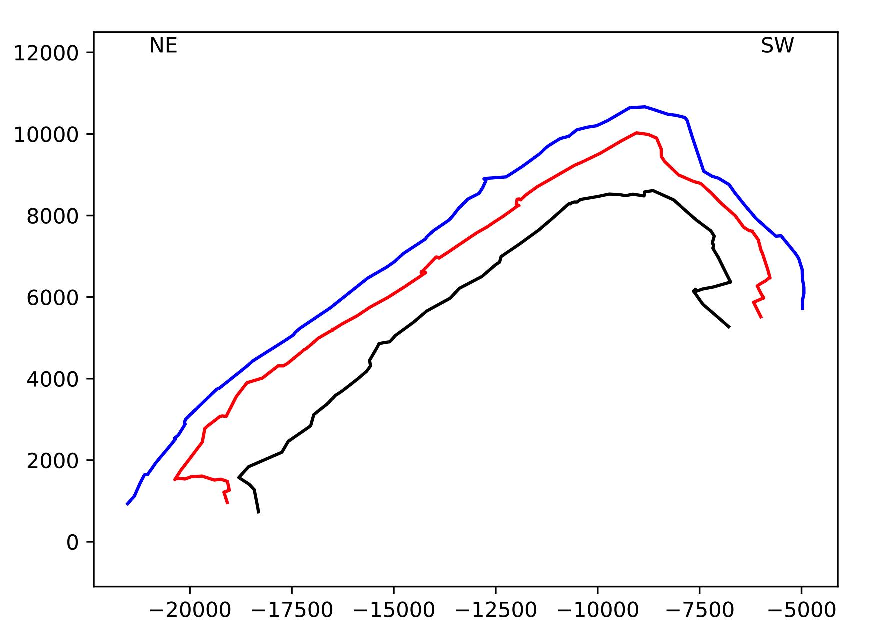
\includegraphics[width=9cm]{ch5f9.pdf}
}}
\end{center}

The thrust verges to the NE (Fig. 5.7), yet the fold verges in the opposite direction to the SW. Unit Jp, between Jtc and Js, contains evaporites. Could this explain the observed fold geometry?

\subsection{Rotations}

Rotations are essential in geology. For example, if from a current lineation on a tilted bed we want to estimate the direction of the current that deposited the bed, we need to rotate the bed (and the lineation) back to their pre-tilting orientation. The stereonet is a convenient device to rotate lines and planes around a horizontal axis or a vertical axis, but it is rather difficult to make rotations around an axis of a different orientation (Marshak and Mitra, 1988). 

A rotation is also a coordinate transformation from an old coordinate system $\mathbf{X_1}\mathbf{X_2}\mathbf{X_3}$ to a new coordinate system $\mathbf{X_1\text{$'$}}\mathbf{X_2\text{$'$}}\mathbf{X_3\text{$'$}}$ (Fig. 5.8). The rotation axis is specified by its trend and plunge, and the magnitude of rotation is given by the angle $\omega$ which is positive for clockwise rotation and vice versa (Fig. 5.8). The difficult part is that the rotation axis may not coincide with the axes of either the old or the new coordinate system (unlike the down-plunge projection).

The components of the transformation matrix \textbf{a} defining the rotation, which are the direction cosines of the new coordinate system $\mathbf{X_1\text{$'$}}\mathbf{X_2\text{$'$}}\mathbf{X_3\text{$'$}}$ with respect to the old coordinate system $\mathbf{X_1}\mathbf{X_2}\mathbf{X_3}$, can be found using spherical trigonometry (Allmendinger et al., 2012) or linear algebra as we did before. Here, we give them without proof. If $\cos\alpha$, $\cos\beta$ and $\cos\gamma$ are the direction cosines of the rotation axis in the \textbf{NED} coordinate system (Table 4.1), and $\omega$ is the amount of rotation, the elements of matrix \textbf{a} are:

\begin{equation}
    \begin{gathered}
        a_{11}=\cos\omega+\cos^2\alpha(1-\cos\omega) \\
        a_{12}=-\cos\gamma\sin\omega+\cos\alpha\cos\beta(1-\cos\omega) \\
        a_{13}=\cos\beta\sin\omega+\cos\alpha\cos\gamma(1-\cos\omega) \\
        a_{21}=\cos\gamma\sin\omega+\cos\beta\cos\alpha(1-\cos\omega) \\
        a_{22}=\cos\omega+\cos^2\beta(1-\cos\omega) \\
        a_{23}=-\cos\alpha\sin\omega+\cos\beta\cos\gamma(1-\cos\omega) \\
        a_{31}=-\cos\beta\sin\omega+\cos\gamma\cos\alpha(1-\cos\omega) \\
        a_{32}=\cos\alpha\sin\omega+\cos\gamma\cos\beta(1-\cos\omega) \\
        a_{33}=\cos\omega+\cos^2\gamma(1-\cos\omega)
    \end{gathered}
\end{equation}

The function \href{https://github.com/nfcd/compGeo/blob/master/source/functions/rotate.py}{rotate} rotates a line (\code{trd} and \code{plg}) about a rotation axis (\code{rtrd} and \code{rplg}), an amount $\omega$ (\code{rot}):

\begin{center}
\begin{lstlisting}[language=Python, frame=single]
import numpy as np
from sph_to_cart import sph_to_cart
from cart_to_sph import cart_to_sph

def rotate(rtrd,rplg,rot,trd,plg,ans0):
	"""
	rotate rotates a line by performing a coordinate
	transformation
	
	rtrd = trend of rotation axis
	rplg = plunge of rotation axis
	rot = magnitude of rotation
	trd = trend of the line to be rotated
	plg = plunge of the line to be rotated
	ans0 = A character indicating whether the line 
		to be rotated is an axis (ans0 = "a") or a 
		vector (ans0 = "v")
	trdr and plgr are the trend and plunge of the
		rotated line
	
	NOTE: All angles are in radians
	
	Python function translated from the Matlab function
	Rotate in Allmendinger et al. (2012)
	"""
	# Allocate some arrays
	a = np.zeros((3,3)) #Transformation matrix
	raxis = np.zeros(3) #Dir. cosines of rotation axis
	line = np.zeros(3)	#Dir. cosines of line to be rotated
	liner = np.zeros(3) #Dir. cosines of rotated line
	
	# Convert rotation axis to direction cosines
	raxis[0] , raxis[1], raxis[2] = sph_to_cart(rtrd,rplg)
	
	# Calculate the transformation matrix a for the rotation
	x = 1.0 - np.cos(rot)
	sinrot = np.sin(rot)
	cosrot = np.cos(rot)
	a[0,0] = cosrot + raxis[0]*raxis[0]*x
	a[0,1] = -raxis[2]*sinrot + raxis[0]*raxis[1]*x
	a[0,2] = raxis[1]*sinrot + raxis[0]*raxis[2]*x
	a[1,0] = raxis[2]*sinrot + raxis[1]*raxis[0]*x
	a[1,1] = cosrot + raxis[1]*raxis[1]*x
	a[1,2] = -raxis[0]*sinrot + raxis[1]*raxis[2]*x
	a[2,0] = -raxis[1]*sinrot + raxis[2]*raxis[0]*x
	a[2,1] = raxis[0]*sinrot + raxis[2]*raxis[1]*x
	a[2,2] = cosrot + raxis[2]*raxis[2]*x
	
	# Convert trend and plunge of line to be rotated into
	# direction cosines
	line[0] , line[1], line[2] = sph_to_cart(trd,plg)
	
	# Perform the coordinate transformation
	for i in range(3):
		for j in range(3):
			liner[i] = a[i,j]*line[j] + liner[i]
	
	# Convert to lower hemisphere projection if axis 
	if liner[2] < 0.0 and ans0 == 'a':
		liner *= -1.0
		
	# Convert from direction cosines back to trend and plunge
	trdr , plgr = cart_to_sph(liner[0], liner[1], liner[2])
	
	return trdr, plgr
\end{lstlisting}
\end{center}

The  notebook  \href{https://github.com/nfcd/compGeo/blob/master/source/notebooks/ch5-5.ipynb}{ch5-5} illustrates  the  use  of  the  function \code{rotate} to solve the following problem from Leyshon  and Lisle  (1996): An overturned bed oriented 305/60 (RHR) has sedimentary lineations which indicate the palaeocurrent direction. These pitch at 60NW, with the current flowing up the plunge. Calculate the original trend of the palaeocurrents. 

Besides rotating the lineations back to their pre-tilted orientation, there is an additional challenge in this problem. We need to figure out the orientation of the lineations from their pitch on the bed. We will do this as well using a rotation.

\begin{center}
\begin{lstlisting}[language=Python, frame=single]
import numpy as np
pi = np.pi

# Import functions 
import sys, os
sys.path.append(os.path.abspath("../functions"))
from pole import pole_from_plane
from rotate import rotate
from zero_twopi import zero_twopi

# Strike and dip of bed in radians
strike, dip = np.radians([305, 60]) 

# Pole of bed
rtrd, rplg = pole_from_plane(strike, dip)

# To find the orientation of the lineations
# rotate the strike line clockwise about the 
# pole an amount equal to the pitch

# strike line
trd, plg = strike, 0 

# rotation = pitch in radians
rot = 60 * pi/180 

# orientation of lineations
trdr, plgr = rotate(rtrd,rplg,rot,trd,plg,"a")

# Now we need to rotate the lineations about
# the strike line to their pre-tilted orientation

# The bed is overturned, so it has been rotated 
# pass the vertical. The amount of rotation
# required to restore the bed to its pre-tilted
# orientation is 180- 60 = 120 deg, and it
# should be clockwise
rot = 120 * pi/180 # rotation in radians

# rotate lineations to their pre-tilted orientation
trdl, plgl = rotate(trd,plg,rot,trdr,plgr,"a")

# The current flows up the plunge, 
# so the trend of the paleocurrents is:
trdl = zero_twopi(trdl + pi)
print("Original trend of the paleocurrents = {:.1f}"
      .format(trdl*180/pi))
\end{lstlisting}
\fbox{
\parbox{\textwidth - 2 \fboxsep}{
Original trend of the paleocurrents = 65.0
}}
\end{center}

\subsection{Plotting great and small circles using rotations}

The transformation matrix \textbf{a} that describes the rotation (Eq. 5.17), provides a simple and elegant way to draw great and small circles on a stereonet. As you may suspect from the previous notebook, to draw a great circle, we just need to rotate the strike line of the plane around the pole to the plane in fixed increments (e.g. 1\degree) until completing 180\degree. This is the same as drawing lines on the plane of incrementally larger rake from 0 to 180\degree. To draw a small circle, we just need to rotate a line around the axis of the conic section in fixed increments (e.g. 1\degree\space) until completing 360\degree. Any line making an angle less than 90\degree\space with the axis of rotation will trace a cone, which will plot on the stereonet as a small circle. The functions \href{https://github.com/nfcd/compGeo/blob/master/source/functions/great_circle.py}{great\_circle} and \href{https://github.com/nfcd/compGeo/blob/master/source/functions/small_circle.py}{small\_circle} return the path of a great or small circle on an equal angle or equal area stereonet:

\begin{center}
\begin{lstlisting}[language=Python, frame=single]
import numpy as np
from pole import pole_from_plane
from rotate import rotate
from st_coord_line import st_coord_line

def great_circle(strike,dip,stype):
	"""
	great_circle computes the great circle path of a plane
	in an equal angle or equal area stereonet of unit radius
	
	strike = strike of plane
	dip = dip of plane
	stype = Stereonet type: 0 = equal angle, 1 = equal area
	path = x and y coordinates of points in great circle path
	
	NOTE: strike and dip should be entered in radians.
	
	Python function translated from the Matlab function
	great_circle in Allmendinger et al. (2012)
	"""
	pi = np.pi
	# Compute the pole to the plane. This will be the axis of
	# rotation to make the great circle
	trda, plga = pole_from_plane(strike,dip)
	
	# Now pick the strike line at the intersection of the
	# great circle with the primitive of the stereonet
	trd, plg = strike, 0.0
	
	# To make the great circle, rotate the line 180 degrees
	# in increments of 1 degree
	rot = np.radians(np.arange(0,181,1))
	path = np.zeros((rot.shape[0],2))
	
	for i in range(rot.size):
	# Avoid joining ends of path
		if rot[i] == pi:
			rot[i] = rot[i] * 0.9999
		# Rotate line
		rtrd, rplg = rotate(trda,plga,rot[i],trd,plg,"a")
		# Calculate stereonet coordinates of rotated line
		# and add to great circle path
		path[i,0], path[i,1] = st_coord_line(rtrd,rplg,stype)
	
	return path
\end{lstlisting}
\end{center}

\begin{center}
\begin{lstlisting}[language=Python, frame=single]
import numpy as np
from rotate import rotate
from st_coord_line import st_coord_line
from zero_twopi import zero_twopi

def small_circle(trda,plga,cangle,stype):
	"""
	small_circle computes the paths of a small circle defined
	by its axis and cone angle, for an equal angle or equal
	area stereonet of unit radius
	
	trda = trend of axis
	plga = plunge of axis
	cangle = cone angle
	stype = Stereonet type: 0 = equal angle, 1 = equal area
	path1 and path2 = vectors with the x and y coordinates
		of the points in the small circle paths
	np1 and np2 = Number of points in path1 and path2
	
	NOTE: All angles should be in radians
	
	Python function translated from the Matlab function
	SmallCircle in Allmendinger et al. (2012)
	"""
	pi = np.pi
	# Find where to start the small circle
	if (plga - cangle) >= 0.0:
		trd = trda
		plg = plga - cangle
	else:
		if plga == pi/2.0:
			plga = plga * 0.9999
		angle = np.arccos(np.cos(cangle)/np.cos(plga))
		trd = zero_twopi(trda+angle)
		plg = 0.0
	
	# To make the small circle, rotate the starting line
	# 360 degrees in increments of 1 degree
	rot = np.radians(np.arange(0,361,1))
	path1 = np.zeros((rot.shape[0],2))
	path2 = np.zeros((rot.shape[0],2))
	np1 = np2 = 0
	for i in range(rot.size):
		# Rotate line: The line is considered as a vector
		rtrd , rplg = rotate(trda,plga,rot[i],trd,plg,"v")
		# Calculate stereonet coordinates and add to path
		# If rotated plunge is positive add to 1st path
		if rplg >= 0.0:
			path1[np1,0] , path1[np1,1] = st_coord_line(rtrd,rplg,
				stype)
			np1 += 1
		# Else add to 2nd path
		else:
			path2[np2,0] , path2[np2,1] = st_coord_line(rtrd,rplg,
				stype)
			np2 += 1
	
	return path1, path2, np1, np2
\end{lstlisting}
\end{center}

Normally, stereonets are displayed looking straight down,  with the primitive equal to the horizontal. However, sometimes it is convenient to look at the stereonet in another orientation. For example, one may want to plot data in the plane of a cross section with the view direction perpendicular to the section, or in a down-plunge projection with the view direction parallel to the fold axis. The function \href{https://github.com/nfcd/compGeo/blob/master/source/functions/geogr_to_view.py}{geogr\_to\_view} enables to plot great and small circles on a stereonet of any view direction, by transforming the poles of rotation from \textbf{NED} coordinates to the view direction coordinates:

\begin{center}
\begin{lstlisting}[language=Python, frame=single]
import numpy as np
from sph_to_cart import sph_to_cart
from cart_to_sph import cart_to_sph
from zero_twopi import zero_twopi

def geogr_to_view(trd,plg,trdv,plgv):
	"""
	geogr_to_view transforms a line from NED to View 
	direction coordinates
	trd = trend of line
	plg = plunge of line 
	trdv = trend of view direction 
	plgv = plunge of view direction 
	rtrd and rplg are the new trend and plunge of the line
	in the view direction.
	
	NOTE: Input/Output angles are in radians
	
	Python function translated from the Matlab function
	GeogrToView in Allmendinger et al. (2012)
	"""
	#some constants 
	east = np.pi/2.0
	
	#Make transformation matrix between NED and View Direction
	a = np.zeros((3,3))
	a[2,0], a[2,1], a[2,2] = sph_to_cart(trdv,plgv)
	temp1 = trdv + east
	temp2 = 0.0
	a[1,0], a[1,1], a[1,2] = sph_to_cart(temp1,temp2)
	temp1 = trdv
	temp2 = plgv - east
	a[0,0], a[0,1], a[0,2] = sph_to_cart(temp1,temp2)
	
	#Direction cosines of line
	dc = np.zeros(3)
	dc[0], dc[1], dc[2] = sph_to_cart(trd,plg)
	
	# Transform line
	ndc = np.zeros(3)
	for i in range(3):
		ndc[i] = a[i,0]*dc[0] + a[i,1]*dc[1]+ a[i,2]*dc[2]
	
	# Compute line from new direction cosines
	rtrd, rplg = cart_to_sph(ndc[0],ndc[1],ndc[2])
	
	# Take care of negative plunges
	if rplg < 0.0 :
		rtrd = zero_twopi(rtrd+np.pi)
		rplg = -rplg
	
	return rtrd, rplg
\end{lstlisting}
\end{center}

We can now put these three functions together in a function called \href{https://github.com/nfcd/compGeo/blob/master/source/functions/stereonet.py}{stereonet}, which plots an equal angle or equal area stereonet in any view direction:

\begin{center}
\begin{lstlisting}[language=Python, frame=single]
import numpy as np
import matplotlib.pyplot as plt
from pole import plane_from_pole
from geogr_to_view import geogr_to_view
from small_circle import small_circle
from great_circle import great_circle

def stereonet(trdv,plgv,intrad,stype):
	"""
	stereonet plots an equal angle or equal area stereonet
	of unit radius in any view direction
	
	USE: fig, ax = stereonet(trdv,plgv,intrad,stype)
	
	trdv = trend of view direction
	plgv = plunge of view direction
	intrad = interval in radians between great or small circles
	stype = Stereonet type: 0 = equal angle, 1 = equal area
	
	fig and ax are handles to the figure and axes
	
	NOTE: All angles should be entered in radians
	
	Python function translated from the Matlab function
	Stereonet in Allmendinger et al. (2012)
	"""
	pi = np.pi
	# some constants
	east = pi/2.0
	west = 3.0*east
	
	# Make a figure
	fig, ax = plt.subplots(figsize=(15,7.5))
	
	# Stereonet reference circle
	r = 1.0 # radius of stereonet
	th = np.radians(np.arange(0,361,1))
	x = r * np.cos(th)
	y = r * np.sin(th)
	# Plot stereonet reference circle
	ax.plot(x,y, "k")
	ax.axis ([-1, 1, -1, 1])
	ax.axis ("equal")
	ax.axis("off")
	
	# Number of small circles
	ncircles = int(pi/(intrad*2.0))
	
	# small circles, start at North
	trd = plg = 0.0
	
	# If view direction is not the default
	# transform line to view direction
	if trdv != 0.0 or plgv != east:
		trd, plg = geogr_to_view(trd,plg,trdv,plgv)
	
	# Plot small circles
	for i in range(1,ncircles+1):
		cangle = i * intrad
		path1, path2, np1, np2 = small_circle(trd,plg,cangle,
			stype)
		ax.plot(path1[np.arange(0,np1),0], 
			path1[np.arange(0,np1),1], color="gray",
			linewidth=0.5)
		if np2 > 0:
			ax.plot(path2[np.arange(0,np2),0], 
				path2[np.arange(0,np2),1], color="gray", 
				linewidth=0.5)
	
	# Great circles
	for i in range(ncircles*2+1):
		# Western half
		if i <= ncircles:
			# Pole of great circle
			trd = west
			plg = i * intrad
		# Eastern half
		else:
			# Pole of great circle
			trd = east
			plg = (i-ncircles) * intrad
		# If pole is vertical shift it a little bit
		if plg == east:
			plg = plg * 0.9999
		# If view direction is not the default 
		# transform line to view direction
		if trdv != 0.0 or plgv != east:
			trd, plg = geogr_to_view(trd,plg,trdv,plgv)
		# Compute plane from pole
		strike, dip = plane_from_pole(trd,plg)
		# Plot great circle
		path = great_circle(strike,dip,stype)
		ax.plot(path[:,0],path[:,1],color="gray",linewidth=0.5)
		
	# return figure and axes handles
	return fig, ax
\end{lstlisting}
\end{center}

Now, let's use all these functions to plot the bedding data of the Big Elk anticline (Fig. \ref{fig:bigElkAnticline}) in an equal angle stereonet, looking down and also along the fold axis. The notebook \href{https://github.com/nfcd/compGeo/blob/master/source/notebooks/ch5-6.ipynb}{ch5-6} illustrates this. Notice that we read the strike and dips from the file \href{https://github.com/nfcd/compGeo/blob/master/source/data/ch5-6/beasd.txt}{beasd.txt}:

\begin{center}
\begin{lstlisting}[language=Python, frame=single]
# Import libraries
import numpy as np
import matplotlib.pyplot as plt
pi = np.pi

# Import Stereonet and related functions
import sys, os
sys.path.append(os.path.abspath("../functions"))
from pole import pole_from_plane, plane_from_pole
from great_circle import great_circle
from geogr_to_view import geogr_to_view
from stereonet import stereonet

# Draw a lower hemisphere equal angle stereonet, 
# 10 deg interval grid
trdv, plgv, intrad = np.radians([0, 90, 10]) 
fig, ax = stereonet(trdv,plgv,intrad,0)

# Read the strike-dip data from the Big Elk anticline
beasd=np.loadtxt(os.path.abspath("../data/ch5-6/beasd.txt"))

# Plot the great circles
for i in range(beasd.shape[0]):
    path = great_circle(beasd[i,0]*pi/180,
                        beasd[i,1]*pi/180,0)
    ax.plot(path[:,0], path[:,1], "b", linewidth=0.5)
\end{lstlisting}
\fbox{
\parbox{\textwidth - 2 \fboxsep}{
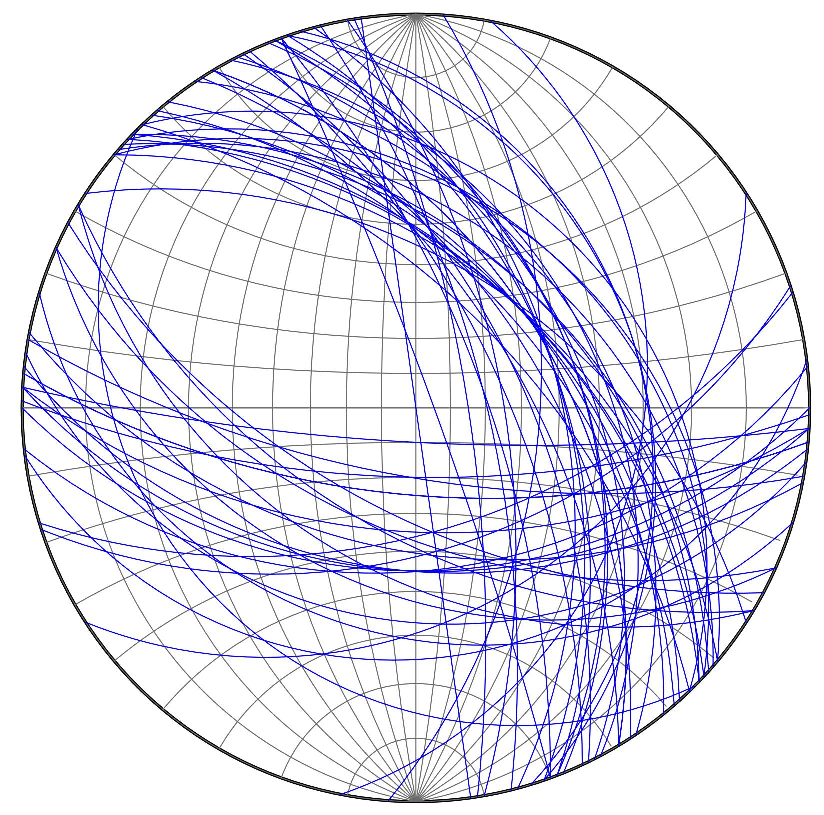
\includegraphics[width=5cm]{ch5f11.pdf}
}}
\end{center}

\begin{center}
\begin{lstlisting}[language=Python, frame=single]
# Draw the same data in an equal angle stereonet,
# but make the view direction = fold axis
trdv, plgv = np.radians([125, 26]) 
fig, ax = stereonet(trdv,plgv,intrad,0)

# Plot the great circles
for i in range(beasd.shape[0]):
    # pole to bed
    trdp, plgp =  pole_from_plane(beasd[i,0]*pi/180,
                                  beasd[i,1]*pi/180)
    # transform pole
    trdpt, plgpt = geogr_to_view(trdp,plgp,trdv,plgv)
    # bed from transformed pole
    striket, dipt = plane_from_pole(trdpt,plgpt)
    # plot great circle
    path = great_circle(striket,dipt,0)
    ax.plot(path[:,0], path[:,1], "b", linewidth=0.5) 
\end{lstlisting}
\fbox{
\parbox{\textwidth - 2 \fboxsep}{
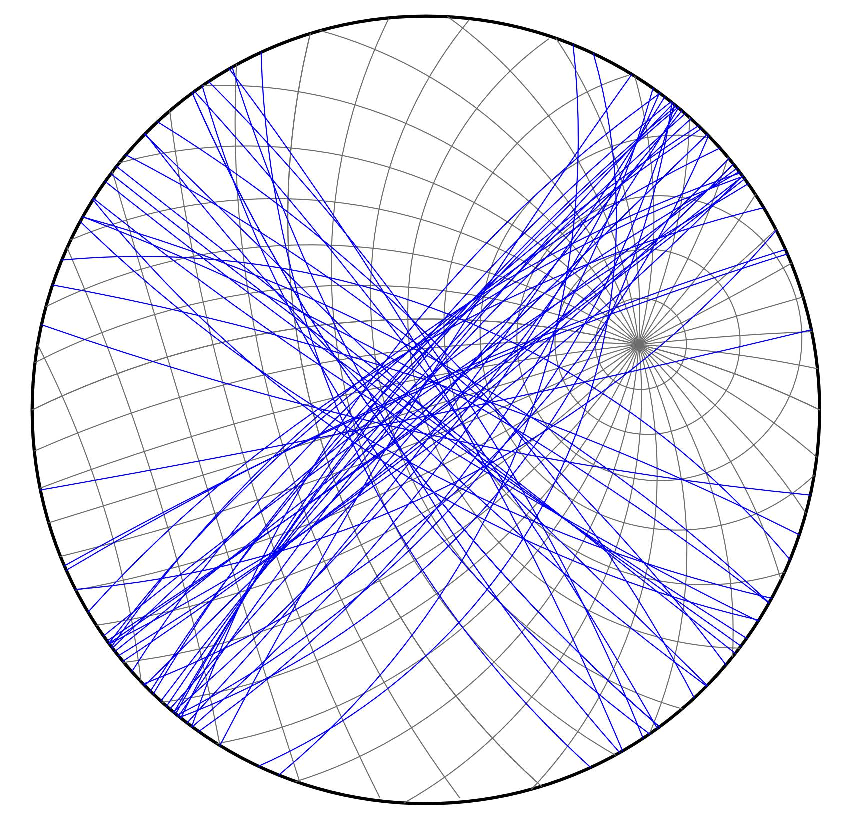
\includegraphics[width=5cm]{ch5f12.pdf}
}}
\end{center}

What do these stereonets tell us about the geometry of the fold?

\section{Exercises}

\begin{enumerate}

    \item Figure 5.8 is a satellite image of the Sheep Mountain anticline, Wyoming, USA (Rioux, 1994). At 75 localities along the anticline in the Jurassic Sundance Formation (gray-green sandstone, siltstone and shale), the \textbf{ENU} coordinates of points on the base and top of the unit (Fig. 5.8a, green and red points), and three points on a bed inside the unit (Fig. 5.8b, blue points), were recorded. You can visualize these points in Google Earth using the file \href{https://github.com/nfcd/compGeo/blob/master/source/data/ch5-exercise1/sdtp.kml}{sdtp.kml}. 
    
    \begin{figure}[ht]
    \centering
    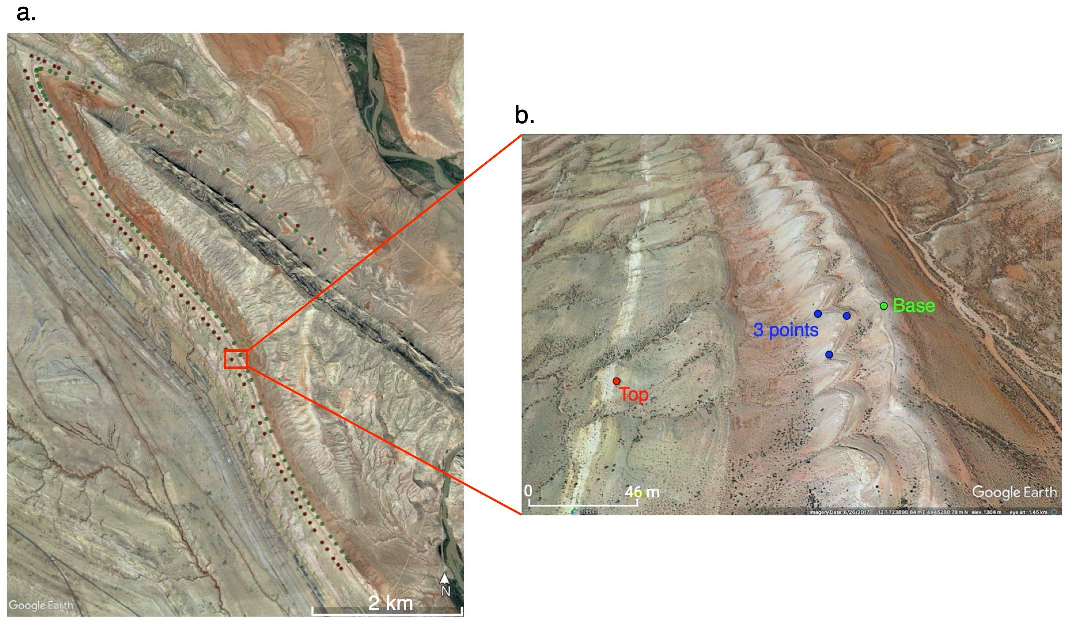
\includegraphics[width=14cm]{ch5f13.pdf}
    \caption{\textbf{a.} Base (green) and top (red) locations of the Jurassic Sundance Formation along the Sheep Mountain anticline, Wyoming. \textbf{b.} Closeup of one of the localities (red rectangle in a) showing as well three points (blue) on one bed.}
    \label{fig: SheepMountain}
    \end{figure}
    
    The file \href{https://github.com/nfcd/compGeo/blob/master/source/data/ch5-exercise1/sdtp.txt}{sdtp.txt} contains the \textbf{ENU} coordinates (UTM in meters) of the points. Each row is one locality, and it contains 15 columns corresponding to the coordinates of points 1 to 5. Points 1 to 3 are on a bed inside the unit, and points 4 and 5 are on the base and top of the unit, respectively. Columns 1 to 3 are the \textbf{ENU} coordinates of point 1, columns 4 to 6 those of point 2, etc. 
    
    \begin{enumerate}
        \item Compute the thickness of the Sundance Formation at the 75 localities. Notice that at each locality you will need to compute the strike and dip using points 1-3 and the \code{three\_points} function, and the thickness using points 4 and 5 and the \code{true\_thickness} function.
        \item Plot the bedding data along the anticline in and equal area, lower hemisphere stereonet. Plot these data as great circles.
        \item Suppose that the error in the horizontal (\textbf{EN}) coordinates is $\pm$ 3 m and in the vertical (\textbf{U}) is $\pm$ 1.5 m. These are conservative error estimates. What are the errors in strike and dip and thickness at the 75 localities? \textit{Hint}: Use functions \code{three\_points\_u} and \code{true\_thickness\_u}.
        \item Make a graph of computed thickness versus computed dip, and another graph of computed thickness versus north (\textbf{N}) for the 75 localities. Include the thickness and dip error bars. Do you see any correlation between thickness and bedding dip? Is there a systematic variation of thickness along the anticline?  
        \item The axis of the anticline is oriented 306/11. This is approximately the location where the bedding planes on the stereonet intersect. In the next chapter we will see how to compute this axis. Make a down-plunge projection of the base and top of the Jurassic Sundance Formation. \textit{Hint}: Project the 75 base and top localities using the function \code{down\_plunge}.
    \end{enumerate}
    
    \item Allmendinger and Judge (2013) discuss the uncertainty in thickness measurements and its implication for estimating the shortening of fold and thrust belts. Figure 5.9 is a geologic map of the Canmore east half area in Alberta, Canada (Price, 1970). The yellow dots are the points used by these authors to estimate the thickness of the Devonian Palliser (Dpa) and Mississippian Livingstone (Mlv) formations. These are in a homoclinal dip package in a thrust sheet. 
    
    The files \href{https://github.com/nfcd/compGeo/blob/master/source/data/ch5-exercise2/dpa.txt}{dpa.txt} and \href{https://github.com/nfcd/compGeo/blob/master/source/data/ch5-exercise2/mlv.txt}{mlv.txt} contain the \textbf{ENU} coordinates (UTM in meters) of the points in the Palliser (Dpa) and Livingstone (Mlv) formations. Each row in the files is one locality, and it contains 12 columns corresponding to the coordinates of points 1 to 4. Points 1-3 are either on the top or the base of the unit, and point 4 is on the other contact. Columns 1 to 3 are the \textbf{ENU} coordinates of point 1, columns 4 to 6 those of point 2, etc.
    
    \begin{enumerate}
        \item Compute the thickness of the Palliser and Livingstone formations at the localities shown in Figure 5.9. What is the mean value of thickness of these two units? What is the standard deviation? \textit{Hint}: Use the functions \code{three\_points} and \code{true\_thickness}. The NumPy functions \code{mean} and \code{std} compute the mean and standard deviation of an array.
        \item Consider that the uncertainty in horizontal and vertical coordinates is $\pm$15.24 m. Compute again the mean value and standard deviation of the thickness of the units. This time these values will have uncertainties. \textit{Hint}: Use the functions \code{three\_points\_u} and \code{true\_thickness\_u}. Notice that you can also use the NumPy functions \code{mean} and \code{std} on arrays of numbers with uncertainties.
        \item How do your results compare to those of Allmendinger and Judge (2013, their Table 1)?
    \end{enumerate}{}
    
    \begin{SCfigure}[][ht]
        \caption{Geologic map of the Canmore east half area, Alberta, Canada (Price, 1970) for exercise 2. The yellow dots are points used to determine the thickness of the Devonian Palliser (Dpa) and Mississippian Livingstone (Mlv) formations.}
        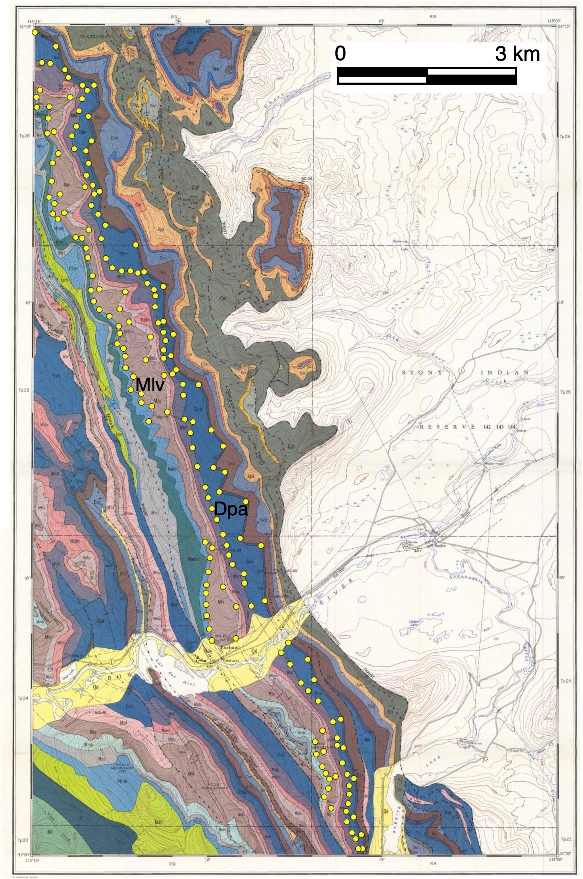
\includegraphics[width=0.5\textwidth]{ch5f14.pdf}
    \end{SCfigure}
    
    \item The following exercise is from Ragan (2009): With the following information and the topographic map of Fig. 5.10, construct a geologic map. The base of a 100 m thick sandstone unit of early Triassic age is exposed at point A; its attitude is 110/25 (RHR). Point B is on the east boundary of a 50 m thick, vertical diabase dike of Jurassic age; its trend is 020. At point C the base of a horizontal Cretaceous sequence is exposed, and at point D the base of a conformable sequence of Tertiary rocks is present.
    
    \begin{figure}[ht]
    \centering
    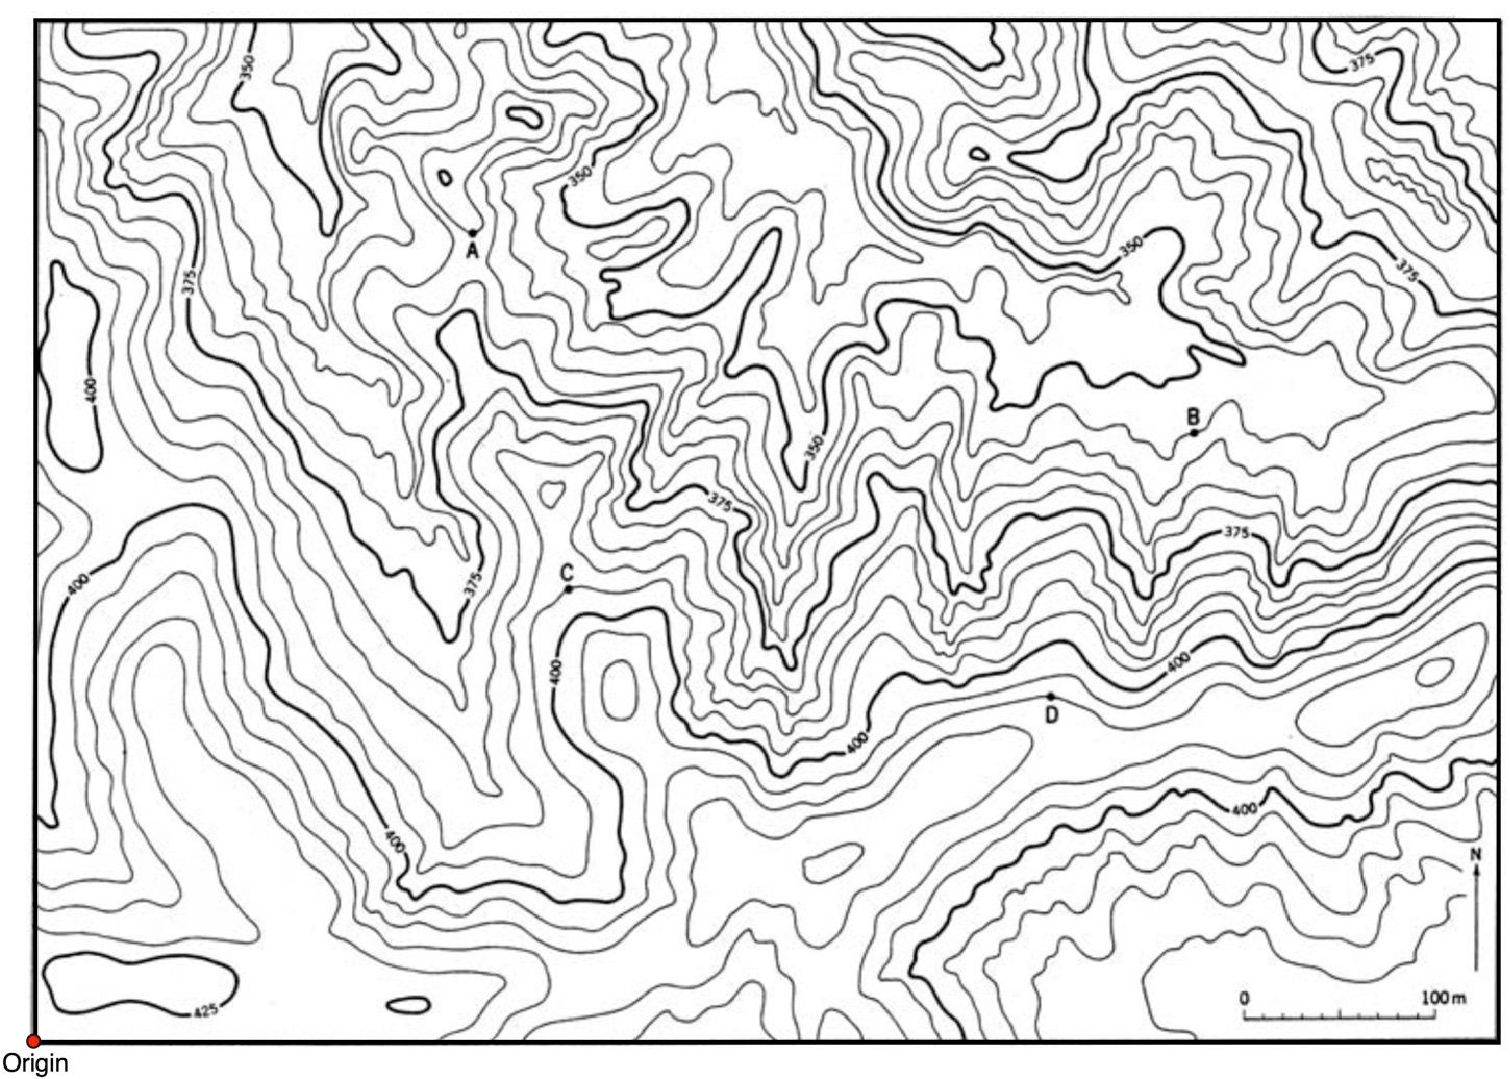
\includegraphics[width=13.5cm]{ch5f15.pdf}
    \caption{Topographic map for exercise 3. Notice that the origin is at the lower left corner of the map. This is exercise 2 in chapter 4 of Ragan (2009).}
    \end{figure}
    
    This exercise is normally solved graphically (Fig. \ref{fig:outrace}. Here, we'll use computation. The files \href{https://github.com/nfcd/compGeo/blob/master/source/data/ch5-exercise3/XGE.txt}{XGE.txt}, \href{https://github.com/nfcd/compGeo/blob/master/source/data/ch5-exercise3/YGE.txt}{YGE.txt}, and \href{https://github.com/nfcd/compGeo/blob/master/source/data/ch5-exercise3/ZGE.txt}{ZGE.txt} are the \textbf{ENU} coordinates of the points of the DEM grid (these arrays follow the format of the NumPy \code{meshgrid} function). Points A, B, C and D have the following \textbf{ENU} coordinates:
    
    A = [232, 428, 370]
    
    B = [612, 322, 355]
    
    C = [281.5, 239, 395]
    
    D = [537, 183, 410]
    
    \textit{Hint}: Use the function \code{outcrop\_trace} to compute the contacts. Follow a procedure similar to notebook \href{https://github.com/nfcd/compGeo/blob/master/source/notebooks/ch5-3.ipynb}{ch5-3}. In this case though, some contacts will intersect. At contacts intersections you will need to determine which contact cuts the other: e.g. the Jurassic dyke will cut the Triassic sequence, but it will be covered by the Cretaceous and Tertiary sequences.
    
    \item This exercise is from Marshak and Mitra (1988). It is hard to solve using a stereonet. Here, you will use the function \code{rotate} to solve it:
    
    In eastern New York, there is an important unconformity called the Taconic unconformity. It separates Mid-Ordovician flysch from Devonian limestone. At a locality near the town of Catskill, the limestone (and the unconformity) is oriented 195/44 (RHR). An anticline occurs in the underlying flysch. One limb is presently oriented 240/73 (limb 1), and the other limb is presently oriented 020/41 (limb 2) (RHR). Flute casts occur in the Ordovician strata on limb 1 (NW dipping limb) and they have an orientation of 037/52.
    
    \begin{enumerate}
        \item What was the orientation of each of the two fold limbs before tilting of the unconformity? \textit{Hint}: Rotate the pole of the unconformity about the strike line of the unconformity to make it vertical. Apply the same rotation to the poles of the limbs and the flute casts. Find the orientation of the limbs from their rotated poles.
        \item What was the orientation of the fold axis prior to tilting? \textit{Hint}: The fold axis is the intersection of the limbs before tilting of the unconformity. Use the module \code{angles} to solve this. 
        \item What was the trend of the current direction responsible for the formation of the flute casts in Ordovician time? \textit{Hint}: Rotate the fold axis computed in (b) about a horizontal line perpendicular to it, to bring it to the horizontal. Apply the same rotation to the poles of the limbs and the flute casts. Then, rotate the poles of the limbs about the horizontal fold axis to make them vertical. Apply the same rotation to the flute casts. If the rotations are correct, the flute casts should be horizontal and their trend is the orientation of the current in the Ordovician.
        \item What is the present orientation of the flute casts on limb 2 (SE dipping limb)? \textit{Hint}: The trend of the flute casts on limb 2 in the Ordovician is the trend you got in (c) minus 180\degree. The plunge of the flute casts is of course zero. Apply to the flute casts on limb 2, the inverse of the rotations you applied to the pole of limb 2 to bring them back to their present orientation.
        \item Plot the results of (a), (b), (c) and (d) as poles and lines on a stereonet. Use colors to indicate the different stages of rotation, and markers to indicate the different elements: unconformity, limbs, fold axis, and flute casts.
    \end{enumerate}{}
    
\end{enumerate}

\addcontentsline{toc}{section}{References}
\section*{References}

Albee, H.F. and Cullins, H.L. 1975. Geologic Map of the Poker Peak Quadrangle, Bonneville County, Idaho. U.S. Geological Survey, Geologic Quadrangle Map GQ 1260. 

Allmendinger, R.W., Cardozo, N. and Fisher, D.W. 2012. Structural Geology Algorithms: Vectors and Tensors. Cambridge University Press.

Ammendinger, R.W. and Judge, P. 2013. Stratigraphic uncertainty and errors in shortening from balanced sections in the North American Cordillera. GSA Bulletin 125, 1569-1579.

Allmendinger, R.W. 2020a. Modern Structural Practice: A structural geology laboratory manual for the 21st century. [\href{https://www.rickallmendinger.net/download}{Online}]. [Accessed March, 2021].

Allmendinger, R.W., 2020b. GMDE: Extracting quantitative information from geologic maps. Geosphere 16, X, 1– 13.

Bennison, G.M., Olver, P.A. and Moseley, K.A. 2011. An Introduction to Geological Structures and Maps, 8th edition. Hodder Education.

Leyshon, P.R. and Lisle, R.J. 1996. Stereographic Projection Techniques in Structural Geology. Butterworth Heinemann.

Marshak, S. and Mitra, G. 1988. Basic Methods of Structural Geology. Prentice Hall.

Price, R.A. 1970. Geology, Canmore (east half), west of Fifth Meridian, Alberta: Geological Survey of Canada “A” Series Map 1265A, scale 1:50,000.

Ragan, D.M. 2009. Structural Geology: An Introduction to Geometrical Techniques. Cambridge University Press.

Rioux, R. L. 1994. Geologic Map of the Sheep Mountain‐Little Sheep Mountain Area, Big Horn County, Wyoming, U.S. Geol. Surv. Open File Rep., 94‐191.

Suppe, J. 1985. Principles of Structural Geology. Prentice-Hall.

% CHAPTER 6: 
\chapter{Tensors}

A tensor is a physical entity that can be transformed from one coordinate system to another, changing its components in a predictable way, but without changing its fundamental nature, such that the tensor is independent of the coordinate system. Thus, scalars (e.g. mass, temperature and density), and vectors (e.g. velocity, force and lines) are tensors. More specifically, scalars are zero order and vectors are first order tensors. In this chapter, we will look at second order tensors which are commonly referred to as \textit{tensors}. This is a short chapter but is fundamental to understand important concepts such as the Mohr circle, the orientation tensor, and the mathematical background for important tensors in geology such as stress and strain.

\section{Basic characteristics of a tensor}

In three dimensions, a \textit{tensor} is characterized by nine components:

\begin{equation}
    \mathbf{T}=T_{ij}=\begin{bmatrix}T_{11}&T_{12}&T_{13}\\T_{21}&T_{22}&T_{23}\\T_{31}&T_{32}&T_{33}\end{bmatrix}
\end{equation}

Notice that tensors are represented by capital bold letters, and we use brackets to differentiate them from matrices such as the transformation matrix \textbf{a} in chapter 5. The nine components of the tensor $T_{ij}$ give the values of the tensor with reference to the three axes of the specific coordinate system $\mathbf{X_1X_2X_3}$. If we change the axes orientations, then the nine components will change but, similar to a vector, the tensor itself will not change.

Like matrices, tensors can be symmetric, asymmetric, or antisymmetric. If the nine components $T_{ij}$ have different values, the tensor is asymmetric. If $T_{ij}=T_{ji}$, the tensor is symmetric. In this case the components above the principal diagonal are the same as those below the diagonal, and only six components are required to define the tensor. Finally, if $T_{ij}=-T_{ji}$, the tensor is antisymmetric. In this case the components along the diagonal are zero, and only three components are required to define the tensor.

Any asymmetric tensor \textbf{T} can be decomposed into a symmetric tensor \textbf{S} plus an antisymmetric tensor \textbf{A}:

\begin{equation}
    T_{ij}=S_{ij}+A_{ij}\quad where\quad S_{ij}=\frac{T_{ij}+T_{ji}}{2}\quad and\quad A_{ij}=\frac{T_{ij}-T_{ji}}{2}
\end{equation}

We will use this property when dealing with infinitesimal strain (chapter 8). 

For all symmetric tensors, there is one orientation of the coordinate axes for which all the components except those along the principal diagonal, are zero:

\begin{equation}
    \mathbf{T}=T_{ij}=\begin{bmatrix}T_{11}&0&0\\0&T_{22}&0\\0&0&T_{33}\end{bmatrix}=\begin{bmatrix}T_2&0&0\\0&T_1&0\\0&0&T_3\end{bmatrix}
\end{equation}

Under this condition, the values along the diagonal are the principal axes of the tensor. Based on their magnitude, these axes are ranked as the maximum ($T_1$), intermediate ($T_2$), and minimum ($T_3$) principal axes. Notice that the indices of the principal axes do not have to coincide with the indices of the coordinate system, for example in Eq. 6.3 $T_1$ is parallel to the coordinate axis $\mathbf{X_2}$. The principal axes define the major, intermediate and minor axes of a three-dimensional surface known as the magnitude ellipsoid (Fig. 6.1). You have probably heard about this ellipsoid before in relation to stress or strain. 

\begin{figure}[ht]
    \centering
    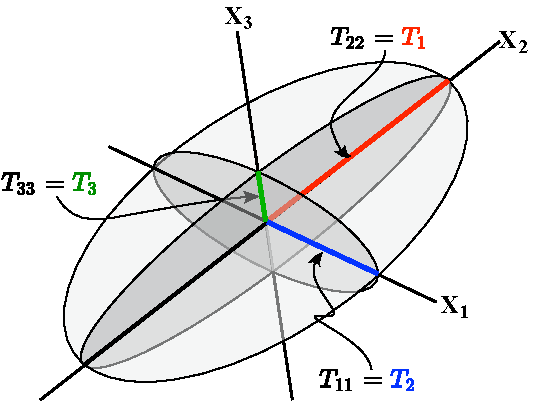
\includegraphics{ch6f1.pdf}
    \caption{The magnitude ellipsoid and principal axes of a symmetric tensor \textbf{T} for the case described by Eq. 6.3. Notice that $T_1$, $T_2$ and $T_3$ define the major, intermediate and minor axes of the ellipsoid. Modified from Allmendinger et al. (2012).}
    \end{figure}
    
\section{Principal axes of a tensor}\label{princAxes}

Determining the orientation of the coordinate system whose axes are parallel to the principal axes of a symmetric tensor involves solving the \textit{eigenvalue} problem (Allmendinger et al., 2012). The mathematical solution to this problem gives a cubic polynomial:

\begin{equation}
    \lambda^3-I\lambda^2-II\lambda-III=0
\end{equation}

The three roots of $\lambda$ are the three eigenvalues and they correspond to the magnitudes of the three principal axes. Once we know the eigenvalues, we can calculate the eigenvectors, which give the orientation of the three principal axes. Thus, we can find the principal axes of any symmetric tensor by finding its eigenvectors and eigenvalues. In Python, the NumPy \code{linalg.eigh} function computes the eigenvalues and eigenvectors of a symmetric array\footnote{\code{eigh} also sorts the eigenvalues in ascending order}. We will use this function later in the chapter when finding the principal axes of a tensor.

The three coefficients $I$, $II$ and $III$ in Eq. 6.4 are known as the invariants of the tensor. They have the same values regardless of the coordinate system we choose. As we will see later (e.g. stress invariants in Chapter 7), these invariants are very important. Their values are given by:

\begin{equation}
    \begin{gathered}
        I=T_{11}+T_{22}+T_{33}=T_1+T_2+T_3 \\
        II=\frac{(T_{ij}T_{ij}-I^2)}{2}=-(T_1T_2+T_2T_3+T_3T_1) \\
        III=\det\mathbf{T}=\vert T_{ij}\vert = T_1T_2T_3 
    \end{gathered}
\end{equation}

\section{Tensors as vector operators}

A tensor commonly relates two vectors, or more formally we can say that a tensor is a linear vector operator because the components of the tensor are the coefficients of a set of linear equations that relate two vectors:

\begin{equation}
    \mathbf{u}=\mathbf{T}\mathbf{v}\quad or\quad u_i=T_{ij}v_j
\end{equation}

A nice example of this relation is Cauchy's law (Chapter 7), which says that the traction on a plane (a vector) is equal to the stress (a tensor) times the pole to the plane (another vector). Since in three dimensions the indices $i$ and $j$ change from 1 to 3, Eq. 6.6 corresponds to three equations, one for each of the components of \textbf{u} in terms of the components of \textbf{v}. In Python this looks like:

\begin{center}
\begin{lstlisting}[language=Python, frame=single]
# v (1 x 3 vector) and T (3 x 3 tensor) are declared before
u = np.zeros(3) # initialize u (1 x 3 vector)
for i in range(3): # free index
    for j in range(3): # dummy index
        u[i] = T[i,j]*v[j] + u[i]
\end{lstlisting}
\end{center}

An implication of Eq. 6.6 is that one can produce a tensor from a type of product of two vectors. This operation is known as the dyad product and it involves multiplying a column vector times a row vector, which gives a 3 x 3 matrix:

\begin{equation}
    \mathbf{T}=\mathbf{u}\otimes\mathbf{v}\quad or\quad T_{ij}=u_iv_j
\end{equation}

This gives nine equations (one for each component of the tensor) in terms of the components of \textbf{u} and \textbf{v}. In Python this looks like:

\begin{center}
\begin{lstlisting}[language=Python, frame=single]
# u (1 x 3 vector) and v (1 x 3 vector) are declared before
T = np.zeros((3,3)) # initialize T (3 x 3 tensor)
for i in range(3): # free index
    for j in range(3): # free index
        T[i,j] = u[i]*v[j]
\end{lstlisting}
\end{center}

In section 6.5, we will use the dyad product to derive the orientation tensor.

\section{Tensor transformations} \label{tensTransf}

If we know the components of a tensor in one coordinate system, we can determine what the components are in any other coordinate system, just as we did with vectors in section \ref{vectortransf}. All we need to know is the transformation matrix \textbf{a}. The procedure, however, is more difficult because a second order tensor is more complicated than a vector. The new components of the tensor in terms of the old are given by (Allmendinger et al., 2012):

\begin{equation}
    \mathbf{T'}=\mathbf{a}^{\mathbf{T}}\mathbf{T}\mathbf{a}\quad or\quad T'_{ij}=a_{ik}a_{jl}T_{kl}
\end{equation}

This equation represent nine equations (since there are two fixed indices $i$ and $j$) with nine terms each (since there are two dummy indices $k$ and $l$). It is tedious to expand and solve Eq. 6.8 by hand. Fortunately, we can solve this equation in Python using loops:

\begin{center}
\begin{lstlisting}[language=Python, frame=single]
# T_old (3 x 3 tensor) and a (3 x 3 transf. matrix) 
# are declared before
T_new = np.zeros((3,3)) # initialize T_new (3 x 3 tensor)
for i in range(3): # free index
    for j in range(3): # free index
        for k in range(3): # dummy index
            for l in range(3): # dummy index
                T_new[i,j] = a[i,k]*a[j,l]*T_old[k,l] \
                    + T_new[i,j]
\end{lstlisting}
\end{center}

Likewise, we can compute the old coordinates of a tensor in terms of the new coordinates:

\begin{equation}
    \mathbf{T}=\mathbf{a}\mathbf{T'}\mathbf{a}^{\mathbf{T}}\quad or\quad T_{ij}=a_{ki}a_{lj}T'_{kl}
\end{equation}

In Python this looks like:

\begin{center}
\begin{lstlisting}[language=Python, frame=single]
# T_new (3 x 3 tensor) and a (3 x 3 transf. matrix) 
# are declared before
T_old = np.zeros((3,3)) # initialize T_old (3 x 3 tensor)
for i in range(3): # free index
    for j in range(3): # free index
        for k in range(3): # dummy index
            for l in range(3): # dummy index
                T_old[i,j] = a[k,i]*a[l,j]*T_new[k,l] \
                    + T_old[i,j]
\end{lstlisting}
\end{center}

\subsection{The Mohr circle}\label{MohrCircle}

Let's consider the case where the axes of the old coordinate system are parallel to the principal axes of the tensor \textbf{T}. Now, let's change the coordinate system to a different orientation by rotating it an angle $\theta$ about one of the principal axes, for example the intermediate axis $T_2$ (Fig. 6.2). The transformation matrix \textbf{a} for this problem is:

\begin{figure}[ht]
    \centering
    \includegraphics{ch6f2.pdf}
    \caption{Rotation of principal coordinate system $\mathbf{X_1X_2X_3}$ about the principal axis $T_2$ an amount $\theta$. Modified from Allmendinger (2020a).}
\end{figure}

\begin{equation}
    \mathbf{a}=\begin{pmatrix}\cos\theta&\cos90&\cos(90-\theta)\\\cos90&\cos0&\cos90\\\cos(90+\theta)&\cos90&\cos\theta\end{pmatrix}=\begin{pmatrix}\cos\theta&0&\sin\theta\\0&1&0\\-\sin\theta&0&\cos\theta\end{pmatrix}
\end{equation}

The tensor \textbf{T} in the old coordinate system is:

\begin{equation}
    \mathbf{T}=T_{ij}=\begin{bmatrix}T_1&0&0\\0&T_2&0\\0&0&T_3\end{bmatrix}
\end{equation}

Now, we can use Eq. 6.8 to calculate the components of the tensor in the new coordinate system. Substituting Eqs. 6.10 and 6.11 into Eq. 6.8 and carrying out the summation, we obtain:

\begin{equation}
    \mathbf{T'}=T'_{ij}=\begin{bmatrix}T_1\cos^2\theta+T_3\sin^2\theta&0&-(T_1-T_3)\sin\theta\cos\theta\\0&T_2&0\\-(T_1-T_3)\sin\theta\cos\theta&0&T_1\sin^2\theta+T_3\cos^2\theta\end{bmatrix}
\end{equation}

The components of $\mathbf{T'}$ can be expressed in a nicer way using the following trigonometric identities for double angles:

\begin{equation}
    \sin 2\theta=2\sin\theta\cos\theta,\quad \sin^2\theta=\frac{1-\cos 2\theta}{2},\quad \cos^2\theta=\frac{1+\cos 2\theta}{2}
\end{equation}

Substituting these equations into Eq. 6.12 and rearranging, we get the following equations for the components of the tensor in the new coordinate system:

\begin{equation}
    \begin{gathered}
        T_{11}'=\frac{T_1+T_3}{2}+\frac{T_1-T_3}{2}\cos 2\theta  \\
        T_{33}'=\frac{T_1+T_3}{2}-\frac{T_1-T_3}{2}\cos 2\theta \\
        T_{13}'=T_{31}'=-\frac{T_1-T_3}{2}\sin 2\theta
    \end{gathered}
\end{equation}

If you recall, the equation of a circle of center $(c,0)$ and radius $r$ is:

\begin{equation}
    \begin{gathered}
        x=c-r\cos\alpha \\
        y=r\sin\alpha
    \end{gathered}
\end{equation}

We can see that these equations are similar to Eq. 6.14. In fact, Eq. 6.14 describes a circle with center $c$ and radius $r$ (Fig. 6.3):

\begin{equation}
    c = \left(\frac{T_1+T_3}{2},0\right)\qquad r = \left(\frac{T_1-T_3}{2}\right)
\end{equation}

\begin{figure}[ht]
    \centering
    \includegraphics{ch6f3.pdf}
    \caption{The Mohr circle is the graphical representation of the rotation of a symmetric tensor about one of its principal axes. Modified from Allmendinger et al. (2012).}
\end{figure}

This circle is known as the \textit{Mohr circle}, because it was devised by the German engineer Otto Mohr in the late 1800s. The Mohr circle is basically a graphical device to rotate a symmetric tensor about one of its principal axes. It is commonly associated with stress, but it can be applied to any symmetric tensor (strain and permeability for example). We will see the application of the Mohr circle in chapters 7 and 8.

\section{The orientation tensor}

The concepts discussed so far in this chapter are the mathematical basis for the following two chapters on stress and strain. We will now focus on a relatively simple yet important problem that relies on the concept of eigenvalues and eigenvectors: How do we find the best-fit fold axis to a group of bedding poles? And similarly, how do we find the best-fit plane to a group of lines?

\subsection{Best-fit fold axis}

The solution to this problem is based on the least squares method (Charlesworth et al., 1976; Allmendinger et al., 2012). Suppose we are trying to calculate the axis $\mathbf{f}$ of a fold. If the fold is truly cylindrical, then all the bedding poles $\mathbf{p}_{[n]}$ should be perpendicular to $\mathbf{f}$, i.e. the angle $\theta_i$ between any pole $\mathbf{p}_{[i]}$ and $\mathbf{f}$ should be 90\degree, and $\cos\theta_i$ should be zero (Fig. 6.4). $\cos\theta_i$ is equal to the dot product between $\mathbf{f}$ and $\mathbf{p}_{[i]}$. Treating these lines as row vectors, the dot product can be written as:

\begin{figure}[ht]
    \centering
    \includegraphics{ch6f4.pdf}
    \caption{Best-fit fold axis to a group of bedding poles. A perfectly oriented pole $\mathbf{p}_{[i]}$ should be perpendicular to the fold axis $\mathbf{f}$, and $\theta_i$ should be 90\degree\space ($\cos\theta_i = 0$). Modified from Allmendinger (2020a).}
\end{figure}

\begin{equation}
    \cos\theta_i=\mathbf{p}_{[i]}\mathbf{f^T}
\end{equation}

We can use the value of $\cos\theta_i$ to represent the deviation of a pole $\mathbf{p}_{[i]}$ from $\mathbf{f}$. The sum of the squares of the deviations of all the poles is:

\begin{equation}
    S=\sum_{i=1}^{n}\cos^2\theta_i=\sum_{i=1}^{n}\left(\mathbf{p}_{[i]}\mathbf{f^T}\right)^2
\end{equation}

Since the dot product is commutative ($\mathbf{p}_{[i]}\mathbf{f^T}=\mathbf{f}\mathbf{p}_{[i]}^{\mathbf{T}} $), we can write Eq. 6.18 as:

\begin{equation}
    S=\sum_{i=1}^{n}\mathbf{f}\mathbf{p}_{[i]}^{\mathbf{T}}\mathbf{p}_{[i]}\mathbf{f^T}=\mathbf{f}\mathbf{T}\mathbf{f^T}
\end{equation}

\textbf{T} is a symmetric tensor known as the \textit{orientation tensor} and is composed of the sum of the dyad products of each pole $\mathbf{p}_{[i]}$ ($[\cos\alpha_i\,\cos\beta_i\,\cos\gamma_i]$) with itself (Eq. 6.7):

\begin{equation}
    \begin{aligned} \mathbf{T} &=\sum_{i=1}^{n} \mathbf{p}_{[i]}^{\mathbf{T}}\mathbf{p}_{[i]}=\sum_{i=1}^{n}\left(p_{i}p_{j}\right)_{[i]} \\ 
    &=\left[\begin{array}{ccc}\sum \cos ^{2} \alpha_{[i]} & \sum \cos \alpha_{[i]} \cos \beta_{[i]} & \sum \cos \alpha_{[i]} \cos \gamma_{[i]} \\ \sum \cos \beta_{[i]} \cos \alpha_{[i]} & \sum \cos ^{2} \beta_{[i]} & \sum \cos \beta_{[i]} \cos \gamma_{[i]} \\ \sum \cos \gamma_{[i]} \cos \alpha_{[i]} & \sum \cos \gamma_{[i]} \cos \beta_{[i]} & \left.\sum \cos ^{2} \gamma_{[i]}\right]\end{array}\right] \end{aligned}
\end{equation}

You can think of $\mathbf{T}$ as describing an ellipsoid in three-dimensions. To find the principal axes of this ellipsoid, we need to calculate the eigenvalues and eigenvectors of $\mathbf{T}$. The smallest eigenvalue of $\mathbf{T}$ is the minimization of the deviations $S$ in Eq. 6.19. If the fold were perfectly cylindrical, the lowest eigenvalue would be zero. Thus, the eigenvector corresponding to the lowest eigenvalue is the best-fit fold axis $\mathbf{f}$.  

The function \href{https://github.com/nfcd/compGeo/blob/master/source/functions/bingham.py}{bingham} computes and plots a cylindrical best-fit to a distribution of bedding poles. It returns the eigenvalues and eigenvectors of $\mathbf{T}$, the uncertainty cones for the Bingham statistics, and the best-fit plane to the bedding poles. For more information on the Bingham statistics, please check Fisher et al. (1987):

\begin{center}
\begin{lstlisting}[language=Python, frame=single]
import numpy as np
import matplotlib.pyplot as plt

from sph_to_cart import sph_to_cart
from cart_to_sph import cart_to_sph
from zero_twopi import zero_twopi
from stereonet import stereonet
from great_circle import great_circle
from st_coord_line import st_coord_line


def bingham(T,P,stype):
	"""
	bingham calculates and plots a cylindrical best fit to
	a distribution of poles to bedding. The statistical
	routine is based on algorithms in Fisher et al. (1988)
	
	USE: eigvec, confcone, bestfit, fig, ax = bingham(T,P)
		
	T and P = Vectors of lines trends and plunges
			respectively
	stype = Stereonet type: 0 = equal angle, 1 = equal area
		
	eigvec = 3 x 3 matrix with eigenvalues (column 1), trends
	(column 2) and plunges (column 3) of the eigenvectors.
	Maximum eigenvalue and corresponding eigenvector are
	in row 1, intermediate in row 2, and minimum in row 3.
	
	confcone = 2 x 2 matrix with the maximum (column 1) and
	minimum (column 2) radius of the 95% elliptical
	confidence cone around the eigenvector corresponding
	to the largest (row 1), and lowest (row 2) eigenvalue
	
	besFit = 1 x 2 vector containing the strike and dip
	(right hand rule) of the best fit great circle to
	the distribution of lines
	
	fig and ax are handles to the figure and axes
	
	NOTE: Input/Output trends and plunges, as well as
	confidence cones are in radians. bingham plots the
	input poles, eigenvectors and best fit great circle
	in an equal area stereonet.
	
	Python function translated from the Matlab function
	Bingham in Allmendinger et al. (2012)
	"""
	# Some constants
	pi = np.pi
	east = pi/2
	twopi = pi*2
	
	# Number of lines
	nlines = len(T)
	
	# Initialize the orientation matrix
	a = np.zeros((3,3))
	
	# Fill the orientation matrix with the sums of the
	# squares (for the principal diagonal) and the products
	# of the direction cosines of each line. cn, ce and cd
	# are the north, east and down direction cosines
	for i in range(0,nlines): 
		cn,ce,cd = sph_to_cart(T[i],P[i])
		a[0,0] = a[0,0] + cn*cn
		a[0,1] = a[0,1] + cn*ce
		a[0,2] = a[0,2] + cn*cd
		a[1,1] = a[1,1] + ce*ce
		a[1,2] = a[1,2] + ce*cd
		a[2,2] = a[2,2] + cd*cd
	
	# The orientation matrix is symmetric so the off-diagonal
	# components can be equated
	a[1,0] = a[0,1]
	a[2,0] = a[0,2]
	a[2,1] = a[1,2]
	
	# Calculate the eigenvalues and eigenvectors of the
	# orientation matrix using function eigh.
	# D is a vector of eigenvalues and V is a full matrix
	# whose columns are the corresponding eigenvectors
	D, V = np.linalg.eigh(a)
	
	# Normalize the eigenvalues by the number of lines and
	# convert the corresponding eigenvectors to the lower
	# hemisphere
	for i in range(0,3): 
		D[i] = D[i]/nlines
		if V[2,i] < 0:
			V[0,i] = -V[0,i]
			V[1,i] = -V[1,i]
			V[2,i] = -V[2,i]
	
	# Initialize eigvec
	eigvec = np.zeros((3,3))
	#Fill eigvec
	eigvec[0,0] = D[2]	  # Maximum eigenvalue
	eigvec[1,0] = D[1]	  # Intermediate eigenvalue
	eigvec[2,0] = D[0]	  # Minimum eigenvalue
	# Trend and plunge of largest eigenvalue: column 3 of V
	eigvec[0,1], eigvec[0,2] = cart_to_sph(V[0,2], V[1,2], 
		V[2,2])
	# Trend and plunge of interm. eigenvalue: column 2 of V
	eigvec[1,1], eigvec[1,2] = cart_to_sph(V[0,1], V[1,1], 
		V[2,1])
	# Trend and plunge of minimum eigenvalue: column 1 of V
	eigvec[2,1], eigvec[2,2] = cart_to_sph(V[0,0], V[1,0], 
		V[2,0])
	
	# Initialize confcone
	confcone = np.zeros((2,2))
	# If there are more than 25 lines, calculate confidence
	# cones at the 95% confidence level. The algorithm is
	# explained in Fisher et al. (1987)
	if nlines >= 25:
		e11 = e22 = e12 = d11 = d22 = d12 = 0
		en11 = 1/(nlines*(eigvec[2,0]-eigvec[0,0])**2)
		en22 = 1/(nlines*(eigvec[1,0]-eigvec[0,0])**2)
		en12 = 1/(nlines*(eigvec[2,0]-eigvec[0,0])*(eigvec[1,0]-
			eigvec[0,0]))
		dn11 = en11
		dn22 = 1/(nlines*(eigvec[2,0]-eigvec[1,0])**2)
		dn12 = 1/(nlines*(eigvec[2,0]-eigvec[1,0])*(eigvec[2,0]-
			eigvec[0,0]))
		vec = np.zeros((3,3))
		for i in range(0,3):
			vec[i,0] = np.sin(eigvec[i,2]+east)*np.cos(twopi-
				eigvec[i,1])
			vec[i,1] = np.sin(eigvec[i,2]+east)*np.sin(twopi-
				eigvec[i,1])
			vec[i,2] = np.cos(eigvec[i,2]+east)
		for i in range(0,nlines):
			c1 = np.sin(P[i]+east)*np.cos(twopi-T[i])
			c2 = np.sin(P[i]+east)*np.sin(twopi-T[i])
			c3 = np.cos(P[i]+east)
			u1x = vec[2,0]*c1 + vec[2,1]*c2 + vec[2,2]*c3
			u2x = vec[1,0]*c1 + vec[1,1]*c2 + vec[1,2]*c3
			u3x = vec[0,0]*c1 + vec[0,1]*c2 + vec[0,2]*c3
			e11 = u1x*u1x * u3x*u3x + e11
			e22 = u2x*u2x * u3x*u3x + e22
			e12 = u1x*u2x * u3x*u3x + e12
			d11 = e11
			d22 = u1x*u1x * u2x*u2x + d22
			d12 = u2x*u3x * u1x*u1x + d12
		e22 = en22*e22
		e11 = en11*e11
		e12 = en12*e12
		d22 = dn22*d22
		d11 = dn11*d11
		d12 = dn12*d12
		d = -2*np.log(.05)/nlines
		# initialize f
		f = np.zeros((2,2))
		if abs(e11*e22-e12*e12) >= 0.000001:
			f[0,0] = (1/(e11*e22-e12*e12)) * e22
			f[1,1] = (1/(e11*e22-e12*e12)) * e11
			f[0,1] = -(1/(e11*e22-e12*e12)) * e12
			f[1,0] = f[0,1]
			# Calculate the eigenvalues and eigenvectors
			# of the matrix f using function eigh
			# The next lines follow steps 1-4 outlined
			# on pp. 34-35 of Fisher et al. (1987)
			DD, _ = np.linalg.eigh(f)
			if DD[0] > 0 and DD[1] > 0:
				if d/DD[0] <= 1 and d/DD[1] <= 1:
					confcone[0,1] = np.arcsin(np.sqrt(d/DD[1]))
					confcone[0,0] = np.arcsin(np.sqrt(d/DD[0]))
		# Repeat the process for the eigenvector
		# corresponding to the smallest eigenvalue
		if abs(d11*d22-d12*d12) >= 0.000001:
			f[0,0] = (1/(d11*d22-d12*d12)) * d22
			f[1,1] = (1/(d11*d22-d12*d12)) * d11
			f[0,1] = -(1/(d11*d22-d12*d12)) * d12
			f[1,0] = f[0,1]
			DD, _ = np.linalg.eigh(f)
			if DD[0] > 0.0 and DD[1] > 0.0:
				if d/DD[0] <= 1 and d/DD[1] <= 1:
					confcone[1,1] = np.arcsin(np.sqrt(d/DD[1]))
					confcone[1,0] = np.arcsin(np.sqrt(d/DD[0]))
	
	# Calculate the best fit great circle
	# to the distribution of points
	bestfit = np.zeros(2)
	bestfit[0] = zero_twopi(eigvec[2,1] + east)
	bestfit[1] = east - eigvec[2,2]
	
	# Plot stereonet
	fig, ax = stereonet(0, 90*pi/180, 10*pi/180, stype)
	
	# Plot lines
	for i in range(0,nlines):
		xp,yp = st_coord_line(T[i],P[i],stype)
		ax.plot(xp,yp,"k.")
	
	# Plot eigenvectors
	for i in range(0,3):
		xp,yp = st_coord_line(eigvec[i,1],eigvec[i,2],stype)
		ax.plot(xp,yp,"rs")
		ax.text(xp-0.03,yp+0.03,str(i+1),c="r")
	
	# Plot best fit great circle
	path = great_circle(bestfit[0],bestfit[1],stype)
	ax.plot(path[:,0],path[:,1],"r")
	
	return eigvec, confcone, bestfit, fig, ax
\end{lstlisting}
\end{center}

Let's use this function to compute the best-fit fold axis for the Big Elk anticline (southeastern Idaho), using the bedding data in Fig. \ref{fig:bigElkAnticline}. The notebook \href{https://github.com/nfcd/compGeo/blob/master/source/notebooks/ch6-1.ipynb}{ch6-1} illustrates this. Notice that the bedding data (strike and dips) are read from the file \href{https://github.com/nfcd/compGeo/blob/master/source/data/ch6-1/beasd.txt}{beasd.txt}:

\begin{center}
\begin{lstlisting}[language=Python, frame=single]
# Import libraries
import numpy as np
import matplotlib.pyplot as plt
pi = np.pi

# Import functions 
import sys, os
sys.path.append(os.path.abspath("../functions"))
from pole import pole_from_plane
from bingham import bingham

# Read the bedding data from the Big Elk anticline
beasd =np.loadtxt(os.path.abspath("../data/ch6-1/beasd.txt"))
# Convert from degrees to radians
beasd = beasd*pi/180

# Initialize poles
T = np.zeros(len(beasd))
P = np.zeros(len(beasd))

# Compute poles to bedding
for i in range(len(T)):
     T[i],P[i] = pole_from_plane(beasd[i,0],beasd[i,1])

# Compute cylindrical best fit
# and plot in equal area stereonet
eigvec,confcone,bestfit, fig, ax = bingham(T,P,1)
# Convert from radians to degrees
eigvec = eigvec * 180/pi
confcone = confcone * 180/pi
bestfit = bestfit * 180/pi

# Print best-fit fold axis
print("Best-fit fold axis: trend = {:.1f}, plunge = {:.1f}"
      .format(eigvec[2,1],eigvec[2,2]))
# Print best-fit plane 
print("Best-fit plane: strike = {:.1f}, dip = {:.1f}\n"
      .format(bestfit[0],bestfit[1]))
# Print confidence cone
print("95% elliptical confidence cones:")
print("Around axis 1: Max = {:.1f}, Min = {:.1f}"
      .format(confcone[0,0],confcone[0,1]))
print("Around axis 3: Max = {:.1f}, Min = {:.1f}"
      .format(confcone[1,0],confcone[1,1]))
\end{lstlisting}
\fbox{
\parbox{\textwidth - 2 \fboxsep}{
\includegraphics[width=5cm]{ch6f5.pdf} \\
Best-fit fold axis: trend = 125.3, plunge 26.1 \\
Best-fit plane: strike = 215.3, dip 63.9 \\
95$\%$ elliptical confidence cones: \\
Around axis 1: Max = 16.9, Min 5.9 \\
Around axis 3: Max = 8.2, Min 5.8
}}
\end{center}

\subsection{Line distributions}

The orientation tensor $\mathbf{T}$ (Eq. 6.20) is also useful for characterizing line distributions. Figure 6.5 shows three end-members of line distributions. The bipolar distribution (Fig. 6.5a) consists of a group of lines that are parallel or sub-parallel to each other and plunge in opposite directions, with some limited scatter. In this case, the lines define an elongate ellipsoid (a cigar), with a large (near 1.0) eigenvalue (long axis of the ellipsoid) and two small (near zero) eigenvalues (short axes of the ellipsoid). Also, the eigenvector of the largest eigenvalue describes well the preferred orientation of the lines (Fig. 6.5a). Notice that in this case, the mean vector calculation (section \ref{MeanVector}) will fail since the lines plunging in opposite directions will cancel each other out.

\begin{figure}[ht]
    \centering
    \includegraphics[width=14cm]{ch6f6.pdf}
    \caption{Three end members of line distributions. \textbf{a.} Bipolar, \textbf{b.} Girdle, and \textbf{c.} random. Each diagram has 30 lines. Modified from Allmendinger (2020a).}
\end{figure}

In the girdle distribution (Fig. 6.5b), all the lines are close to being coplanar, and they define a flattened ellipsoid (or pancake), with one small (near zero) eigenvalue corresponding to the pole of the best-fit plane through the lines, and two large relatively equal eigenvalues (near 0.5) whose eigenvectors lie within the best-fit plane. Finally, in the random distribution (Fig. 6.5c), the lines define a sphere and the eigenvalues are relatively equal. Thus, in general, the eigenvalues of $\mathbf{T}$ are a good way to characterize line distributions.

\subsection{Best-fit plane}

In section \ref{ThreePointProblem} we look at the problem of calculating the orientation of a plane from three points on the plane. But what if we have more than three points on the plane? We can use the least squares approach above to solve this problem (Allmendinger, 2020b). This will also allow us to evaluate the goodness of fit of the plane to the data points. Let's assume the points are defined by position vectors $\mathbf{p}_{[i]}$ in an east-north-up (\textbf{ENU}) coordinate system. First, the centroid $\mathbf{c}$ of the position vectors $\mathbf{p}_{[i]}$ is calculated:

\begin{equation}
    \mathbf{c}=\frac{\sum_{i=1}^{n}\mathbf{p}_{[i]}}{n}
\end{equation}

Then, the centroid $\mathbf{c}$ is subtracted from the position vectors $\mathbf{p}_{[i]}$:

\begin{equation}
    \mathbf{s}_{[i]}=\mathbf{p}_{[i]}-\mathbf{c}
\end{equation}

And we use the vectors $\mathbf{s}_{[i]}$ to construct a covariance matrix $\mathbf{C}$ (which looks very similar to the orientation matrix $\mathbf{T}$):

\begin{equation}
    \mathbf{C}=\left[\begin{array}{ccc}\sum (s_E)_{[i]}^{2}  & \sum (s_E)_{[i]} (s_N)_{[i]} & \sum (s_E)_{[i]} (s_U)_{[i]} \\ \sum (s_N)_{[i]} (s_E)_{[i]} & \sum (s_N)_{[i]}^{2} & \sum (s_N)_{[i]} (s_U)_{[i]} \\ \sum (s_U)_{[i]} (s_E)_{[i]} & \sum (s_U)_{[i]} (s_N)_{[i]} & \sum (s_U)_{[i]}^{2}\end{array}\right]
\end{equation}

Finally, the eigenvalues and eigenvectors of the covariance matrix $\mathbf{C}$ are determined. The eigenvector corresponding to the smallest eigenvalue is the pole to the best-fit plane, and the square root of the smallest eigenvalue is the standard deviation of the distance of each point from the best-fit plane.

The function \href{https://github.com/nfcd/compGeo/blob/master/source/functions/fit_plane.py}{fit\_plane} calculates the best-fit plane to a group of lines:

\begin{center}
\begin{lstlisting}[language=Python, frame=single]
import numpy as np

from pole import plane_from_pole
from cart_to_sph import cart_to_sph

def fit_plane(pts):
	"""
	fit_plane computes the best-fit plane for a group of
	points (position vectors) on the plane
	
	USE: strike, dip, stdev = fit_plane(pts)
	
	pts is a n x 3 matrix containing the East (column 1),
	North (column 2), and Up (column 3) coordinates
	of n points on the plane
	
	strike and dip are returned in radians
	
	stdev is the standard deviation of the distance of
	each point from the best-fit plane
	"""
	# Compute the centroid of the selected points
	avge = np.mean(pts[:,0])
	avgn = np.mean(pts[:,1])
	avgu = np.mean(pts[:,2])
	
	# Compute the points vectors minus the centroid
	pts[:,0] = pts[:,0] - avge
	pts[:,1] = pts[:,1] - avgn
	pts[:,2] = pts[:,2] - avgu
	
	# Compute the covariance/orientation matrix
	a = np.zeros((3,3))
	for i in range(pts.shape[0]):
		ce = pts[i,0]
		cn = pts[i,1]
		cu = pts[i,2]
		# compute orientation matrix
		a[0,0] = a[0,0] + ce*ce
		a[0,1] = a[0,1] + ce*cn
		a[0,2] = a[0,2] + ce*cu
		a[1,1] = a[1,1] + cn*cn
		a[1,2] = a[1,2] + cn*cu
		a[2,2] = a[2,2] + cu*cu
	# The orientation matrix is symmetric so the 
	# off-diagonal components are equal
	a[1,0] = a[0,1]
	a[2,0] = a[0,2]
	a[2,1] = a[1,2]
	
	# calculate the eigenvalues and eigenvectors of the
	# orientation matrix: use function eigh
	D, V = np.linalg.eigh(a)
	
	# Calculate pole to best-fit plane = lowest eigenvalue
	# vector in N, E, D coordinates
	cn = V[1,0]
	ce = V[0,0]
	cd = -V[2,0]
	
	# Find trend and plunge of pole to best fit plane
	trd, plg =cart_to_sph(cn,ce,cd)
	
	# Find Best fit plane
	strike, dip = plane_from_pole(trd,plg)
	
	# Calculate standard deviation = square root of
	# minimum eigenvalue
	stdev = np.sqrt(D[0])
	
	return strike, dip, stdev
\end{lstlisting}
\end{center}

Let's use this function to compute the orientation of the contact between the Jurassic Js and Cretaceous Ke in the northeastern part of the Poker Peak Quadrangle, Idaho (Albee et al., 1975) (yellow contact in Fig. 6.6). The notebook \href{https://github.com/nfcd/compGeo/blob/master/source/notebooks/ch6-2.ipynb}{ch6-2} shows the solution to this problem. Notice that the UTM \textbf{ENU} coordinates of the points on the Js-Ke contact are read from the file \href{https://github.com/nfcd/compGeo/blob/master/source/data/ch6-2/jske.txt}{jske.txt}:

\begin{SCfigure}[][ht]
    \caption{Northeastern portion of the Poker Peak Quadrangle, Idaho (Albee et al., 1975). The yellow dots are points on the Js-Ke contact.}
    \includegraphics[width=0.55\textwidth]{ch6f7.pdf}
\end{SCfigure}

\begin{center}
\begin{lstlisting}[language=Python, frame=single]
# Import libraries
import numpy as np
pi = np.pi

# Import function fit_plane
import sys, os
sys.path.append(os.path.abspath('../functions'))
from fit_plane import fit_plane

# Read the points on the contact
# Coordinates are UTM (ENU) in meters
jske = np.loadtxt(os.path.abspath('../data/ch6-2/jske.txt'))

# Compute best-fit plane
strike, dip, stdev = fit_plane(jske)

# Print strike and dip of plane
print('Strike = {:.1f}, Dip = {:.1f}'
      .format(strike*180/pi,dip*180/pi))

# Print standard deviation of the distance of each point
# from the best-fit plane
print('Standard deviation = {:.1f} m'.format(stdev))
\end{lstlisting}
\fbox{
\parbox{\textwidth - 2 \fboxsep}{
Strike = 153.3, Dip = 29.9 \\
Standard deviation = 246.8 m
}}
\end{center}

This orientation is not far from the strikes and dips close to the Js-Ke contact in Fig. 6.6. To learn more about fitting a plane to a distribution of lines, you can read Fernandez (2005).

\section{Exercises}

\begin{enumerate}
    \item The file \href{https://github.com/nfcd/compGeo/blob/master/source/data/ch6-exercise1/csdtp.txt}{csdtp.txt} contains the strikes and dips (RHR) of the Jurassic Sundance Formation around the Sheep Mountain Anticline, Wyoming (Fig. \ref{fig: SheepMountain}). You can visualize these bedding orientations in Google Earth using the file \href{https://github.com/nfcd/compGeo/blob/master/source/data/ch6-exercise1/csdtp.kml}{csdtp.kml}. Compute the anticline's best-fit fold axis using the function \code{bingham}.
    
    \item The file \href{https://github.com/nfcd/compGeo/blob/master/source/data/ch6-exercise2/biaxial.txt}{biaxial.txt}, \href{https://github.com/nfcd/compGeo/blob/master/source/data/ch6-exercise2/girdle.txt}{girdle.txt}, and \href{https://github.com/nfcd/compGeo/blob/master/source/data/ch6-exercise2/random.txt}{random.txt} contain the lines (trend and plunge) of the distributions shown in Fig. 6.5. Compute the eigenvalues and eigenvectors, and the 95$\%$ confidence cones of these line distributions using the function \code{bingham}.
    
    \item Trede et al. (2019) published an interesting article about the appropriate sample size for strike and dip measurements. Figure 6.7 shows the Lidar scan of one of their test surfaces, a two meters-size foliation in Cambro-Ordovician mica schists of the Svarthola Cave, SW Norway. The file \href{https://github.com/nfcd/compGeo/blob/master/source/data/ch6-exercise3/fol.txt}{fol.txt} contains the \textbf{ENU} coordinates of the scanned points (grey points, Fig. 6.7), and the file \href{https://github.com/nfcd/compGeo/blob/master/source/data/ch6-exercise3/kfol.txt}{kfol.txt} contains the \textbf{ENU} coordinates of regularly spaced points on the foliation (red circles, Fig. 6.7).
    
    \begin{figure}[ht]
    \centering
    \includegraphics[width=11cm]{ch6f8.pdf}
    \caption{Two-meters size foliation plane in Cambro-Ordovician mica schists of the Svarthole Cave, SW Norway. The grey points are Lidar scanned points on the foliation. The red circles are points on a regular grid covering the foliation. The Lidar scan frequency is 300 kHz, and vertical and horizontal point spacing are 0.013 and 0.022 m, respectively. From Trede et al. (2019).}
\end{figure}
    
    \begin{enumerate}
        \item On each of the points of the regularly spaced grid (red points, Fig. 6.7), compute the strike and dip of the foliation using the Lidar scanned points (grey points, Fig. 6.7) within a radius $r$ of 0.1 m from the grid point. Do this only if there are more than 3 points within the radius $r$.
        \item Repeat the procedure in (a) for larger radii $r$ of 0.3, 0.5, 0.7 and 0.9 m.
        \item Plot histograms of the strike, and of the dip, for each value of $r$. Vertically stack the histograms starting with $r$ = 0.1 at the base. Use different colors to denote the different $r$ values (see Fig. 8 of Trede et al., 2019).
        \item At what radius $r$, does the orientation of the foliation stabilize? What is the best sample size to measure the foliation?
    \end{enumerate}
    
    \textit{Hint}: Use function \code{fit\_plane}.
    
\end{enumerate}

\section*{References}

Albee, H.F. and Cullins, H.L. 1975. Geologic Map of the Poker Peak Quadrangle, Bonneville County, Idaho. U.S. Geological Survey, Geologic Quadrangle Map GQ 1260.

Allmendinger, R.W., Cardozo, N. and Fisher, D.M. 2012. Structural Geology Algorithms: Vectors and Tensors. Cambridge University Press.

Allmendinger, R.W. 2020a. Modern Structural Practice: A structural geology laboratory manual for the 21st century. [\href{https://www.rickallmendinger.net/download}{Online}]. [Accessed March, 2021].

Allmendinger, R.W., 2020b. GMDE: Extracting quantitative information from geologic maps. Geosphere 16, X, 1– 13.

Charlesworth, H.A.K., Langenberg, C.W. and Ramsden, J. 1976. Determining axes, axial planes, and sections of macroscopic folds using computer-based methods. Canadian Journal of Earth Science 13, 54-65.

Fernandez, O. 2005. Obtaining a best fitting plane through 3D georeferenced data. Journal of Structural Geology 27, 855–858.

Fisher, N.I., Lewis, T. and Embleton, B.J.J. 1987. Statistical analysis of spherical data. Cambridge University Press.

Trede, C., Cardozo, N. and Watson, L. 2019. What is the appropriate sample size for strike and dip measurements? An evaluation from compass, smartphone and LIDAR measurements. Norwegian Journal of Geology 99, 1-14.

% CHAPTER 7:
\chapter{Stress}

Geoscientists and engineers are familiar with the concept of stress (other people too). Stress describes the forces per unit area, i.e. the tractions, acting on imaginary planes of varied orientations inside a body. These tractions and the stress occur at a particular instant of time. 

\section{The stress tensor}

A traction is defined as a force, \textbf{f}, divided by the area of the plane, A, on which it acts:

\begin{equation}
    \mathbf{t}=\frac{\mathbf{f}}{A}
\end{equation}

A force of one Newton acting on one square meter is one Pascal (1 N/\SI{}{\metre\squared} = 1 Pa). A Pascal is very small, the atmospheric pressure is about $10^5$ Pa. Therefore, we use a more convenient unit called Megapascal (1 MPa = $10^6$ Pa). 

In the subsurface, the vertical traction due to the weight of the overburden ($\sigma_v$) is equal to:

\begin{equation}\label{eq7.2}
    \sigma_v=\rho g h
\end{equation}

where $\rho$ is the rock density, $g$ is gravity, and $h$ is depth. Rock density increases with depth, but assuming an average rock density of 2400 kg/\SI{}{\metre\cubed}, $\sigma_v$ is about 24 MPa at 1 km depth. 23-25 MPa/km is a reasonable value for the gradient of $\sigma_v$ with depth.

If we now consider a point in space and a Cartesian coordinate system $\mathbf{X_1X_2X_3}$ centered at this point (Fig. 7.1), the components of the stress tensor, $\boldsymbol{\sigma}$, are just the tractions on planes that are perpendicular to the axes of the coordinate system:

\begin{equation}
    \sigma_{ij}=\begin{bmatrix}\sigma_{11}&\sigma_{12}&\sigma_{13}\\\sigma_{21}&\sigma_{22}&\sigma_{23}\\\sigma_{31}&\sigma_{32}&\sigma_{33}\end{bmatrix}
\end{equation}

\begin{figure}[ht]
    \centering
    \includegraphics[width=9cm]{ch7f1.pdf}
    \caption{The components of the stress tensor are the normal and shear tractions on planes perpendicular to the coordinate axes.}
\end{figure}

For each component, the first index indicates the axis perpendicular to the plane, and the second index the axis to which the traction is parallel (Fig. 7.1). Tractions with equal indices (e.g. $\sigma_{11}$) act perpendicular to the plane and are called normal tractions, while tractions with different indices (e.g. $\sigma_{12}$) act parallel to the plane and are called shear tractions. Because normal tractions are predominantly compressive within the Earth (Eq. 7.2), in geology we consider compressive normal tractions as positive and tensional normal tractions as negative. This is opposite to material science, where tensional normal tractions are considered positive.

From Fig. 7.1 it is also clear that if the cube is in equilibrium and it does not rotate about one of the coordinates axis, the stress tensor must be symmetric ($\sigma_{ij}=\sigma_{ji}$).

\subsection{Cauchy's law}

The stress tensor relates two vectors, the traction on a plane, $\mathbf{t}$, and the pole to the plane, $\mathbf{p}$ (Fig. 7.2). This is nicely expressed by Cauchy's law (for a proof of this law see Allmendinger et al., 2012):

\begin{equation}
    t_i=\sigma_{ij}p_j
\end{equation}

\begin{figure}[ht]
    \centering
    \includegraphics[width=8.5cm]{ch7f2.pdf}
    \caption{Tractions $t_i$ on a plane oblique to the coordinate axes. $\mathbf{p}$ is the pole to the plane.}
\end{figure}

Notice that $t_i$ are tractions parallel to the axes of the coordinate system and $\mathbf{p}$ is a unit vector defined by its direction cosines with respect to these axes (Fig. 7.2).

The function \href{https://github.com/nfcd/compGeo/blob/master/source/functions/cauchy.py}{cauchy} calculates the tractions $t_i$ on a plane of any orientation in any coordinate system. \code{cauchy} uses function \href{https://github.com/nfcd/compGeo/blob/master/source/functions/dircos_axes.py}{dircos\_axes} which calculates the direction cosines of the $\mathbf{X_1X_2X_3}$ axes. To define the orientation of these axes, it is just necessary to give the trend and plunge of $\mathbf{X_1}$ and the trend of $\mathbf{X_3}$:

\begin{center}
\begin{lstlisting}[language=Python, frame=single]
import numpy as np

from dircos_axes import dircos_axes
from sph_to_cart import sph_to_cart
from pole import pole_from_plane

def cauchy(stress,tx1,px1,tx3,strike,dip):
	"""
	Given the stress tensor in a X1X2X3 coordinate system,
	cauchy computes the X1X2X3 tractions on an arbitrarily
	oriented plane 
	
	USE: t,pt = cauchy(stress,tx1,px1,tx3,strike,dip)
	
	stress = 3 x 3 stress tensor
	tx1 = trend of X1
	px1 = plunge of X1
	tx3 = trend of X3
	strike = strike of plane
	dip = dip of plane
	t = 1 x 3 vector with X1, X2 and X3 tractions
	pt = 1 x 3 vector with direction cosines of pole
		to plane with respect to X1X2X3
	
	NOTE = Plane orientation follows the right hand rule
	Input/Output angles are in radians
	
	Python function translated from the Matlab function
	Cauchy in Allmendinger et al. (2012)
	"""
	# Compute direction cosines of X1X2X3 with respect
	# to NED
	dc = dircos_axes(tx1,px1,tx3)
	
	# Calculate direction cosines of pole to plane
	trd, plg = pole_from_plane(strike,dip)
	p = np.zeros(3)
	p[0],p[1],p[2] = sph_to_cart(trd,plg)
	
	# Transform pole to plane to stress coordinates X1X2X3
	# The transformation matrix is the direction cosines of
	# X1X2X3
	pt = np.zeros(3)
	for i in range(3):
		for j in range(3):
			pt[i] = dc[i,j]*p[j] + pt[i]
			
	# Calculate the tractions in stress coordinates X1X2X3
	t = np.zeros(3)
	# Compute tractions using Cauchy"s law
	for i in range(3):
		for j in range(3):
			t[i] = stress[i][j]*pt[j] + t[i]
	
	return t, pt
\end{lstlisting}
\end{center}

\begin{center}
\begin{lstlisting}[language=Python, frame=single]
import numpy as np

from sph_to_cart import sph_to_cart

def dircos_axes(tx1,px1,tx3):
	"""
	dircos_axes calculates the direction cosines of a right
	handed, orthogonal X1X2X3 cartesian coordinate system
	of any orientation with respect to NED
	
	USE: dc = dircos_axes(tx1,px1,tx3)
	
	tx1 = trend of X1
	px1 = plunge of X1
	tx3 = trend of X3
	dc = 3 x 3 matrix containing the direction cosines
		of X1 (row 1), X2 (row 2), and X3 (row 3)
	
	Note: Input angles should be in radians
	
	Python function translated from the Matlab function
	DirCosAxes in Allmendinger et al. (2012)
	"""
	# Some constants
	east = np.pi/2.0
	west = 3.0*east
	# tolerance for near zero values
	tol = 1e-6 
	
	# Initialize matrix of direction cosines
	dc = np.zeros((3,3))
	
	# Direction cosines of X1
	dc[0,0],dc[0,1],dc[0,2] = sph_to_cart(tx1,px1)
	
	# Calculate plunge of axis 3
	# If axis 1 is horizontal
	if abs(px1) < tol:
		dt = abs(tx1-tx3)
		if abs(dt - east) < tol or abs(dt - west) < tol:
			px3 = 0.0
		else:
			px3 = east
	# Else
	else:
		# Since dot product X1 and X3 = 0
		px3 = np.arctan(-(dc[0,0]*np.cos(tx3)
			+dc[0,1]*np.sin(tx3))/dc[0,2])
	
	# Direction cosines of X3
	dc[2,0],dc[2,1],dc[2,2] = sph_to_cart(tx3,px3)
	
	# X2 is the cross product of X3 and X1
	dc[1,:] = np.cross(dc[2,:],dc[0,:])
	# Make it a unit vector
	dc[1,:] = dc[1,:]/np.linalg.norm(dc[1,:])
	
	return dc
\end{lstlisting}
\end{center}

\subsection{Stress transformation}

If we know the components of the stress tensor in one coordinate system $\mathbf{X_1X_2X_3}$, we can calculate the components of the tensor in another coordinate system $\mathbf{X'_1X'_2X'_3}$ (section \ref{tensTransf}):

\begin{equation}
    \boldsymbol{\sigma '}=\mathbf{a}^{\mathbf{T}}\boldsymbol{\sigma}\mathbf{a}\quad \text{or}\quad \sigma'_{ij}=a_{ik}a_{jl}\sigma_{kl}
\end{equation}

where $\mathbf{a}$ is the transformation matrix between the new and the old coordinate system. The function \href{https://github.com/nfcd/compGeo/blob/master/source/functions/transform_stress.py}{transform\_stress} tranforms the stress tensor from one coordinate system to another:

\begin{center}
\begin{lstlisting}[language=Python, frame=single]
import numpy as np
from dircos_axes import dircos_axes

def transform_stress(stress,tx1,px1,tx3,ntx1,npx1,ntx3):
	"""
	transform_stress transforms a stress tensor from
	old X1X2X3 to new X1'X2'X3' coordinates
	
	nstress=transform_stress(stress,tx1,px1,tx3,ntx1,npx1,ntx3)
	
	stress = 3 x 3 stress tensor
	tx1 = trend of X1 
	px1 = plunge of X1 
	tx3 = trend of X3
	ntx1 = trend of X1'
	npx1 = plunge of X1'
	ntx3 = trend of X3'
	nstress = 3 x 3 stress tensor in new coordinate system
	
	NOTE: All input angles should be in radians
	
	Python function translated from the Matlab function
	TransformStress in Allmendinger et al. (2012)
	"""
	# Direction cosines of axes of old coordinate system
	odc = dircos_axes(tx1,px1,tx3)
	
	# Direction cosines of axes of new coordinate system
	ndc = dircos_axes(ntx1,npx1,ntx3)
	
	# Transformation matrix between old and new
	# coordinate systems
	a = np.zeros((3,3))
	for i in range(3):
		for j in range(3):
			# Use dot product
			a[i,j] = np.dot(ndc[i,:],odc[j,:])
	
	# Transform stress
	nstress = np.zeros((3,3))
	for i in range(3):
		for j in range(3):
			for k in range(3):
				for l in range(3):
					nstress[i,j] = a[i,k] * a[j,l] * stress[k,l] \
						+ nstress[i,j]
	
	return nstress
\end{lstlisting}
\end{center}

\subsection{Principal axes of stress}

Since stress is a symmetric tensor, there is one orientation of the coordinate system for which the non-diagonal components of the tensor are zero, and only normal tractions act on the planes perpendicular to the coordinate axes (Fig. 7.3). These normal tractions are the principal stresses: $\sigma_1$ is the maximum, $\sigma_2$ is the intermediate, and $\sigma_3$ is the minimum principal stress.

\begin{figure}[ht]
    \centering
    \includegraphics[width=8.5cm]{ch7f3.pdf}
    \caption{Plane oblique to the principal stress coordinate system $\mathbf{X_1X_2X_3}$. $\sigma_1$, $\sigma_2$ and $\sigma_3$ are the principal stresses, and $\sigma$ and $\tau$ are the normal and maximum shear tractions on the plane.}
\end{figure}

As we saw in section \ref{princAxes}, finding the principal stresses is an eigenvalue problem. The function \href{https://github.com/nfcd/compGeo/blob/master/source/functions/principal_stress.py}{principal\_stress} calculates the principal stresses and their orientations for a given stress tensor in a Cartesian coordinate system of any orientation:

\begin{center}
\begin{lstlisting}[language=Python, frame=single]
import numpy as np

from dircos_axes import dircos_axes
from cart_to_sph import cart_to_sph

def principal_stress(stress,tx1,px1,tx3):
	"""
	Given the stress tensor in a X1X2X3 coordinate system
	principal_stress calculates the principal stresses and
	their orientations (trend and plunge) 
	
	USE: pstress,dcp = principal_stress(stress,tx1,px1,tx3)
	
	stress = Symmetric 3 x 3 stress tensor
	tx1 = trend of X1
	px1 = plunge of X1
	tx3 = trend of X3
	pstress = 3 x 3 matrix containing the magnitude
		(column 1), trend (column 2), and plunge
		(column 3) of the	 maximum (row 1),
		intermediate (row 2), and minimum (row 3)
		principal stresses
	dcp = 3 x 3 matrix with direction cosines of the
		principal stress directions: Max. (row 1),
		Int. (row 2), and Min. (row 3) with respect
		to North-East-Down
	
	NOTE: Input/Output angles are in radians
	
	Python function translated from the Matlab function
	PrincipalStress in Allmendinger et al. (2012)
	"""
	# Compute direction cosines of X1X2X3
	dc = dircos_axes(tx1,px1,tx3)
	
	# Initialize pstress
	pstress = np.zeros((3,3))
	
	# Calculate the eigenvalues and eigenvectors
	# of the stress tensor
	D, V = np.linalg.eigh(stress)
	
	# Fill principal stress magnitudes
	pstress[0,0] = D[2] # Maximum principal stress
	pstress[1,0] = D[1] # Interm. principal stress
	pstress[2,0] = D[0] # Minimum principal stress
	
	# The direction cosines of the principal stresses are
	# with respect to the X1X2X3 stress coordinate system,
	# so they need to be transformed to the NED coordinate
	# system
	tv = np.zeros((3,3))
	for i in range(3):
		for j in range(3):
			for k in range(3):
				tv[j,i] = dc[k,j]*V[k,i] + tv[j,i]
				
	
	# Initialize dcp
	dcp = np.zeros((3,3))
	
	# Direction cosines of principal stresses
	for i in range(0,3):
		for j in range(0,3):
			dcp[i,j] = tv[j,2-i]
		# Avoid precision issues
		# Make sure the principal axes are unit vectors
		dcp[i,:] = dcp[i,:]/np.linalg.norm(dcp[i,:])
	
	# Trend and plunge of principal stresses
	for i in range(0,3):
		pstress[i,1],pstress[i,2] = cart_to_sph(dcp[i,0],
			dcp[i,1],dcp[i,2])
	
	return pstress,dcp
\end{lstlisting}
\end{center}

If we know the principal stresses, and the direction cosines of the pole to the plane $\mathbf{p}$  with respect to them (Fig. 7.3), it is possible to compute the normal, $\sigma$, and maximum shear, $\tau$, tractions acting on the plane (Ramsay, 1967):

\begin{equation}
    \begin{gathered}
        \sigma=\sigma_{1} l^{2}+\sigma_{2} m^{2}+\sigma_{3} n^{2} \\
        \tau^{2}=\left(\sigma_{1}-\sigma_{2}\right)^{2} l^{2} m^{2}+\left(\sigma_{2}-\sigma_{3}\right)^{2} m^{2} n^{2}+\left(\sigma_{3}-\sigma_{1}\right)^{2} n^{2} l^{2}
    \end{gathered}
\end{equation}

where $l$, $m$ and $n$ are the direction cosines of $\mathbf{p}$ with respect to $\sigma_1$, $\sigma_2$ and $\sigma_3$, respectively. Notice that this equation just tells us about the magnitude of the maximum shear traction. It does not say anything about the direction and sense of it. In section \ref{shearOnPlane}, we will see a more comprehensive way to solve this problem.

Let's use the functions introduced so far to solve the following problem: The maximum, intermediate and minimum principal stresses are 40, 30, and 20 MPa, respectively. $\sigma_1$ is vertical and $\sigma_3$ is horizontal and trends N-S:

\begin{enumerate}
    \item Compute the tractions parallel to the principal stress directions, acting on a plane with orientation 040/65 (RHR).
    \item Compute the normal and maximum shear tractions acting on the plane
    \item Compute the stress tensor on a new coordinate system with $\mathbf{X_1}$ 030/45 and $\mathbf{X_3}$ trending 210.
    \item Demonstrate that these new components represent still the same tensor, by computing the principal stresses from the new components.
\end{enumerate}

The notebook \href{https://github.com/nfcd/compGeo/blob/master/source/notebooks/ch7-1.ipynb}{ch7-1} shows the solution to this problem:

\begin{center}
\begin{lstlisting}[language=Python, frame=single]
# Import libraries
import numpy as np
pi = np.pi

# Import Cauchy, TransformStress and PrincipalStress
import sys, os
sys.path.append(os.path.abspath("../functions"))
from cauchy import cauchy 
from transform_stress import transform_stress
from principal_stress import principal_stress

# Stress tensor in principal stress coordinate system
stress = np.array([[40, 0, 0],[ 0, 30, 0],[ 0, 0, 20]])

# trend and plunge of X1, and trend of X3
tx1, px1, tx3 = np.radians([0, 90, 0])

# plane orientation
strike, dip = np.radians([40, 65])

# X1, X2 and X3 tractions on the plane
t,pt = cauchy(stress,tx1,px1,tx3,strike,dip)
print("X1, X2 and X3 tractions = ", t.round(3),"\n")

# Compute the normal and maximum shear tractions 
# on the plane: Eq. 7.6
l2 = pt[0]**2
m2 = pt[1]**2
n2 = pt[2]**2
s1 = stress[0,0]
s2 = stress[1,1]
s3 = stress[2,2]
s12 = s1 - s2
s23 = s2 - s3
s31 = s3 - s1
sigma = s1*l2 + s2*m2 + s3*n2
tau = np.sqrt(s12*s12*l2*m2 + s23*s23*m2*n2 + s31*s31*n2*l2)
print("Sigma = {:.3f}, Tau = {:.3f}\n".format(sigma,tau))

# New coordinate system
# trend and plunge of X"1,and trend of X"3
ntx1, npx1, ntx3 = np.radians([30, 45, 210])

# Transform stress to new coordinate system
nstress = transform_stress(stress,tx1,px1,tx3,ntx1,npx1,ntx3)
print("Stress in new coord. system = \n", 
      nstress.round(3),"\n")

# Principal stresses from new components
pstress, dcp = principal_stress(nstress,ntx1,npx1,ntx3)
pstress[:,1:3] = pstress[:,1:3]*180/pi
print("Sigma1 = {:.3f}, Trend = {:.1f}, Plunge = {:.1f}"
      .format(pstress[0,0],pstress[0,1],pstress[0,2]))
print("Sigma2 = {:.3f}, Trend = {:.1f}, Plunge = {:.1f}"
      .format(pstress[1,0],pstress[1,1],pstress[1,2]))
print("Sigma3 = {:.3f}, Trend = {:.1f}, Plunge = {:.1f}"
      .format(pstress[2,0],pstress[2,1],pstress[2,2]))
\end{lstlisting}
\fbox{
\parbox{\textwidth - 2 \fboxsep}{
X1, X2 and X3 tractions =  [16.905 20.828 11.651] \\
Sigma = 28.392, Tau = 7.015 \\
Stress in new coordinate system = \\
\*[[31.25 3.062 8.75] \\
\*[3.062 27.5 -3.062] \\
\*[8.75 -3.062 31.25]] \\ 
Sigma1 = 40.000, Trend = 149.0, Plunge = -90.0 \\
Sigma2 = 30.000, Trend = 270.0, Plunge = -0.0 \\
Sigma3 = 20.000, Trend = 180.0, Plunge = 0.0
}}
\end{center}

The principal stresses computed from the new components of the stress tensor are the same as the input principal stresses. Try changing the orientations of the principal stresses in the notebook (e.g. \code{tx1} = 45, \code{px1} = 0). Check how the results change. This is a great way to understand the concepts introduced so far.

\section{Mohr circle for stress}

As discussed in section \ref{MohrCircle}, the Mohr circle is derived by making a rotation about one of the principal axes of a symmetric tensor. In the case of stress, the rotation is about one of the principal stresses. In Figure 7.4a, the old axes are parallel to the principal axes of the stress tensor, and the rotation is about the $\mathbf{X_2}$ ($\sigma_2$) axis. If the amount of rotation $\theta$ is such that the new $\mathbf{X'_1}$ axis is parallel to the normal to the plane $\mathbf{n}$ (Fig. 7.4b), the components $\sigma '_{11}$ and $\sigma '_{13}$ are the normal ($\sigma$) and shear ($\tau$) tractions on the plane, respectively. These tractions are given by:

\begin{equation}
    \begin{gathered}
        \sigma=\frac{\sigma_1+\sigma_3}{2}+\frac{\sigma_1-\sigma_3}{2}\cos2\theta \\
        \tau=\frac{\sigma_1-\sigma_3}{2}\sin2\theta
    \end{gathered}
\end{equation}

which are similar to Eq. 6.14\footnote{The sign change in the equation for $\tau$ is due to our convention of considering compressional tractions as positive.} and define the Mohr circle for stress. 

\begin{figure}[ht]
    \centering
    \includegraphics[width=15cm]{ch7f4.pdf}
    \caption{Rotation of the stress tensor about $\mathbf{X_2}$. \textbf{a.} The old coordinate system is parallel to the principal axes of the tensor. \textbf{b.} In the new coordinate system $\mathbf{X'_1}$ is parallel to the normal to the plane of interest. Modified from Allmendinger et al. (2012).} 
\end{figure}

The horizontal axis of the Mohr circle for stress is $\sigma$ and the vertical axis is $\tau$. $\sigma$ is positive if compressional, and $\tau$ is positive if the sense of shear is anticlockwise (e.g. Fig. 7.4b). The x coordinate of the center, $C$, of the Mohr circle is $(\sigma_1+\sigma_3)/2$, and the radius, $r$, is $(\sigma_1-\sigma_3)/2$ (Fig. 7.5).

\begin{figure}[ht]
    \centering
    \includegraphics[width=14cm]{ch7f5.pdf}
    \caption{Mohr circle for stress for the situation shown in Fig. 7.4. The normal and shear tractions on the plane (point $P$) can be found by either measuring $2\theta$ from $\sigma_1$ or by tracing the plane from the pole of planes $O_P$.} 
    \label{fig:poleOfPlanes}
\end{figure}

If the normal to the plane makes an angle $\theta$ with respect to $\sigma_1$ (Fig. 7.4), the normal and shear tractions on the plane can be found by drawing in the Mohr circle a radius $CP$ at an angle $2\theta$ with respect to $\sigma_1$ (Fig. 7.5). The coordinates of point $P$ are the normal and shear tractions on the plane.

If we draw lines from $\sigma_1$ and $\sigma_3$ parallel to the planes on which these tractions act, the lines will intersect at a point $O_P$ (Fig. 7.5). This point is known as the pole for planes (Ragan, 2009) and it has a very useful property: A line drawn from $O_P$ to any point $P$ on the Mohr circle circumference is parallel to the plane on which the tractions given by $P$ act (Fig. 7.5). Thus, from $O_P$, we can rapidly find out the tractions on any plane parallel to $\sigma_2$. 

Notice that we can rotate the stress tensor about anyone of the three principal axes. Thus in 3D, the Mohr circle for stress consists of three circles, each one describing the rotation about one of the principal stresses. In section \ref{3DMohrCircle} we will see how to plot the Mohr circle for stress in 3D.

\subsection {Special states of stress}

There are some special states of stress that can be illustrated with the Mohr circle:

\begin{itemize}
    \item Biaxial stress: Two of the principal stresses are non-zero and are different (Fig. 7.6a).
    \item Triaxial stress: This is the most general type of stress. It has three non-zero, different principal stresses (Fig. 7.6b).
    \item Cylindrical stress: When two of the principal stresses are equal and the third is different (Fig. 7.6c). If the two equal principal stresses are zero, the stress is known as uniaxial.
    \item Hydrostatic stress: All three principal stresses have the same value (Fig. 7.6d). In this case, any direction is a principal axis (the stress tensor is a sphere), and there are no shear tractions on the body. This condition is typical of static fluids.
    \item Pure shear stress: Two of the principal stresses are equal in magnitude but opposite in sign (one is compressional and the other is tensional), and the third is zero (Fig. 7.6e).
\end{itemize}

\begin{figure}[ht]
    \centering
    \includegraphics[width=14cm]{ch7f6.pdf}
    \caption{Mohr circle for several special states of stress. \textbf{a.} Biaxial, \textbf{b.} Triaxial, \textbf{c.} Cylindrical uniaxial, \textbf{d.} Hydrostatic, \textbf{e.} Pure shear. Modified from Allmendinger et al. (2012).} 
\end{figure}

\section{Mean and deviatoric stress}\label{meanDevStress}

The special states of stress above allow us to introduce two fundamental types of stress tensors, the mean stress and the deviatoric stress. The mean traction is the average of the three normal tractions (the elements in the diagonal of the stress tensor):

\begin{equation}
    \sigma_m=\frac{\sigma_{11}+\sigma_{22}+\sigma_{33}}{3}
\end{equation}

Notice that the mean traction is the same regardless of the coordinate system because the sum of the normal tractions is the first invariant of the stress tensor (section \ref{princAxes}). Knowing the mean traction, we can express the stress tensor as the sum of two tensors:

\begin{equation}
    \sigma_{ij}=\left[\begin{array}{ccc}\sigma_m & 0 & 0 \\ 0 & \sigma_m & 0 \\ 0 & 0 & \sigma_m\end{array}\right]+\left[\begin{array}{ccc}\sigma_{11}-\sigma_m & \sigma_{12} & \sigma_{13} \\ \sigma_{21} & \sigma_{22}-\sigma_m & \sigma_{23} \\ \sigma_{31} & \sigma_{32} & \sigma_{33}-\sigma_m\end{array}\right]
\end{equation}

The tensor on the left is the mean stress. It is a hydrostatic state of stress that may cause a body to shrink or expand but, on first glance, it is difficult to see how it would change the shape of the body, unless the body is heterogeneous in strength. The tensor on the right is the deviatoric stress. It is the part of the stress tensor that causes distortion of the body. For a cylindrical state of stress (Fig. 7.6c), it is easy to visualize these tensors. The mean stress is represented by the center of the Mohr circle, while the deviatoric stress is represented by the same circle but centered at the origin.

\section{Applications}

In this section we will look at a problem involving stress, namely calculating the magnitude and orientation of the normal and maximum shear tractions on a plane. This problem is crucial to any question involving faulting and fracturing in the upper crust. We will also use the proposed solution to draw the Mohr circle for stress in 3D.

\subsection{Normal and shear tractions on a plane}\label{shearOnPlane}

Figure 7.7 illustrates the problem. We want to determine the normal and maximum shear tractions on a plane of any orientation, under a stress tensor with principal axes of any orientation. There are three coordinate systems involved: 1. The geographic coordinate system $\mathbf{NED}$ where the data are input and the results are output, 2. The principal stress coordinate system which is defined by the orientation of the principal stresses $\sigma_1$, $\sigma_2$ and $\sigma_3$, and 3. A coordinate system defined by the fault plane, with the pole to the plane, $\mathbf{p}$, as the first axis, the line of zero shear traction on the fault plane, $\mathbf{b}$, as the second axis, and the line of maximum shear traction on the fault plane, $\mathbf{s}$, as the third axis.

\begin{figure}[ht]
    \centering
    \includegraphics[width=8cm]{ch7f7.pdf}
    \caption{Lower hemisphere, equal area stereonet illustrating the three coordinate systems involved in determining the maximum shear traction on a fault plane with pole $\mathbf{p}$. These coordinate systems are: $\mathbf{NED}$, $\sigma_1\sigma_2\sigma_3$, and $\mathbf{pbs}$. $\mathbf{b}$ and $\mathbf{s}$ are the directions of zero and maximum shear traction, respectively. Modified from Allmendinger et al. (2012).} 
\end{figure}

The solution to this problem consists of the following steps:

\begin{enumerate}
    \item Transform the stress tensor to principal stress coordinates. Here we can use the function \code{principal\_stress}.
    \item Transform the pole to the plane $\mathbf{p}$ to principal stress coordinates.
    \item Compute the traction vector $\mathbf{t}$ (Fig. 7.7) in principal stress coordinates using Cauchy's law (Eq. 7.4).
    \item $\mathbf{p}$, $\mathbf{t}$ and the maximum shear traction $\mathbf{s}$ fall along the same plane (Fig. 7.7). This plane is known as the \textit{movement plane} (Marshak and Mitra, 1988). The pole to the movement plane is the line of zero shear traction $\mathbf{b}$. Therefore, we can calculate $\mathbf{b}$ by the cross product of $\mathbf{t}$ and $\mathbf{p}$, and $\mathbf{s}$ by the cross product of $\mathbf{p}$ and $\mathbf{b}$. 
    \item Make a transformation matrix $\mathbf{a}$ between the principal stress coordinates and the fault plane coordinates. This matrix has as the first row $\mathbf{p}$, the second row $\mathbf{b}$, and the third row $\mathbf{s}$.
    \item Transform the stress tensor from principal stress coordinates to fault plane coordinates. For the transformed tensor, $\mathbf{X'_1}$ is the pole to the plane $\mathbf{p}$, and $\mathbf{X'_3}$ is the direction of the maximum shear traction $\mathbf{s}$. Therefore, $\sigma'_{11}$ is the normal traction on the plane, and $\sigma'_{13}$ is the maximum shear traction on the plane.
    \item Transform $\mathbf{p}$, $\mathbf{b}$ and $\mathbf{s}$ from principal stress coordinates to $\mathbf{NED}$ coordinates and find their orientations (trend and plunge).
\end{enumerate}

The function \href{https://github.com/nfcd/compGeo/blob/master/source/functions/shear_on_plane.py}{shear\_on\_plane} follows these steps and computes the normal and maximum shear tractions on a plane of any orientation, and under a stress tensor of any orientation:

\begin{center}
\begin{lstlisting}[language=Python, frame=single]
import numpy as np
from principal_stress import principal_stress
from sph_to_cart import sph_to_cart
from cart_to_sph import cart_to_sph
from pole import pole_from_plane

def shear_on_plane(stress,tx1,px1,tx3,strike,dip):
	"""
	shear_on_plane calculates the direction and magnitudes of
	the normal and maximum shear tractions on an arbitrarily
	oriented plane
	
	tt,dctt,srat=shear_on_plane(stress,tx1,px1,tx3,strike,dip)
	
	stress = 3 x 3 stress tensor
	tx1 = trend of X1
	px1 = plunge of X1
	tx3 = trend of X3
	strike = strike of plane
	dip = dip of plane
	tt = 3 x 3 matrix with the magnitude (column 1),
		trend (column 2) and plunge (column 3) of the:
		normal traction on the plane (row 1), zero shear
		traction (row 2), and max. shear traction (row 3)
	dctt = 3 x 3 matrix with the direction cosines of unit
		vectors parallel to: normal traction on the plane
		(row 1), zero shear traction (row 2), and maximum
		shear traction (row 3) with respect to NED
	srat = stress ratio
	
	NOTE = Input stress tensor does not need to be along
		principal stress directions
		Plane orientation follows the right hand rule
		Input/Output angles are in radians
	
	Python function translated from the Matlab function
	shear_on_plane in Allmendinger et al. (2012)
	"""
	# Compute principal stresses and their orientations
	pstress, dcp = principal_stress(stress,tx1,px1,tx3)
	
	# Update stress tensor to principal stress directions
	stress = np.zeros((3,3))
	for i in range(3):
		stress[i,i] = pstress[i,0]
	
	# Calculate stress ratio
	srat = (stress[1,1]-stress[0,0])/(stress[2,2]-stress[0,0])
	
	# Calculate direction cosines of pole to plane
	trd, plg = pole_from_plane(strike,dip)
	p = np.zeros(3)
	p[0], p[1], p[2] = sph_to_cart(trd,plg)
	
	# transform pole to plane to  principal stress coordinates
	pt = np.zeros(3)
	for i in range(3):
		for j in range(3):
			pt[i] = dcp[i,j]*p[j] + pt[i]
	
	# Calculate the tractions in principal stress coordinates
	t = np.zeros(3)
	# Compute tractions using Cauchy's law
	for i in range(3):
		for j in range(3):
			t[i] = stress[i,j]*pt[j] + t[i]
	
	# Find the b axis by the cross product of t and pt
	b = np.cross(t,pt)
	
	# Find the max. shear traction orientation
	# by the cross product of pt and b
	s = np.cross(pt,b)
	
	# Convert b and s to unit vectors
	b = b/np.linalg.norm(b)
	s = s/np.linalg.norm(s)
	
	# Now we can write the transformation matrix from
	# principal stress coordinates to plane coordinates
	a = np.zeros((3,3))
	a[0,:] = pt
	a[1,:] = b
	a[2,:] = s
	
	# Transform stress from principal to plane coordinates
	# Do it only for the first row since we are just
	# interested in the plane: sigma'11 = normal traction,
	# sigma'12 = zero, and sigma'13 = max. shear traction
	tt = np.zeros((3,3))
	for i in range(3):
		tt[i,0] = stress[0,0]*a[0,0]*a[i,0] \
		+ stress[1,1]*a[0,1]*a[i,1] + stress[2,2]*a[0,2]*a[i,2]
	
	# Transform normal traction, zero shear
	# and max. shear traction to NED coords
	dctt = np.zeros((3,3))
	for i in range(3):
		for j in range(3):
			dctt[0,i] = dcp[j,i]*pt[j] + dctt[0,i]
			dctt[1,i] = dcp[j,i]*b[j] + dctt[1,i]
			dctt[2,i] = dcp[j,i]*s[j] + dctt[2,i]
	
	# Compute trend and plunge of normal traction,
	# zero shear, and max. shear traction on plane
	for i in range(3):
		tt[i,1],tt[i,2] = cart_to_sph(dctt[i,0],
			dctt[i,1],dctt[i,2])
	
	return tt, dctt, srat
\end{lstlisting}
\end{center}

The function \code{shear\_on\_plane} also computes an important parameter called the principal stress ratio, $R$ (\code{srat} in the function):

\begin{equation}
    R=\frac{(\sigma_2-\sigma_1)}{(\sigma_3-\sigma_1)}
\end{equation}

when $R$ is 1, $\sigma_2$ is equal to $\sigma_3$; when $R$ is 0, $\sigma_2$ is equal to $\sigma_1$. This ratio is of key importance for predicting faulting and fracturing in the crust (Gephart, 1990; Morris and Ferrill, 2009). Let's look at the influence of this parameter for the case illustrated in Figure 7.7. Let's assume $\sigma_1 = 50$ MPa and $\sigma_3 = 10$ MPa, and let's vary $\sigma_2$ between $\sigma_3$ ($R=1$) and $\sigma_1$ ($R=0$). The notebook \href{https://github.com/nfcd/compGeo/blob/master/source/notebooks/ch7-2.ipynb}{ch7-2} shows the solution to this problem:

\begin{center}
\begin{lstlisting}[language=Python, frame=single]
# Import libraries
import numpy as np
import matplotlib.pyplot as plt
pi = np.pi

# Import functions
import sys, os
sys.path.append(os.path.abspath("../functions"))
from shear_on_plane import shear_on_plane
from great_circle import great_circle
from st_coord_line import st_coord_line

# Stress tensor in principal stress coordinate system
# start with R = 1, sigma2 = sigma3
stress = np.array([[50, 0, 0],[ 0, 10, 0],[ 0, 0, 10]])

# Trend and plunge of sigma1, and trend of sigma3
tx1, px1, tx3 = np.radians([325, 33, 66])

# Plane orientation
strike, dip = np.radians([320, 40])

# Number of R increments
rinc = 11

# sigma2 increment
sstep = (stress[0,0] - stress[2,2])/(rinc-1)

# Initialize array
nort = np.zeros(rinc) # normal tractions
sht = np.zeros(rinc) # max. shear traction
tsht = np.zeros(rinc) # trend max. shear traction
psht = np.zeros(rinc) # plunge max. shear traction
rval = np.zeros(rinc) # R value

# Compute normal and shear tractions for all Rs
for i in range(0,rinc):
    stress[1,1] = stress[2,2] + sstep*i
    # Compute normal and maximum shear tractions on plane
    tt,dctt,srat = shear_on_plane(stress,tx1,px1,
                                  tx3,strike,dip)
    # Extract values
    nort[i] = tt[0,0]
    sht[i] = tt[2,0]
    tsht[i] = tt[2,1]
    psht[i] = tt[2,2]
    rval[i] = srat

# Make a larger figure
fig, ax = plt.subplots(1,2,figsize=(15,6))
    
# Plot fault plane and max. shear tractions
# orientations in a lower hemisphere, equal 
# area stereonet

# Plot the primitive of the stereonet
r = 1; # unit radius
th = np.arange(0,361,1)*pi/180
x = r * np.cos(th)
y = r * np.sin(th)
ax[0].plot(x,y,"k")
# Plot center of circle
ax[0].plot(0,0,"k+")
# Make axes equal and remove them
ax[0].axis("equal")
ax[0].axis("off")
# Plot fault plane
path = great_circle(strike,dip,1)
ax[0].plot(path[:,0], path[:,1], "k") 
# Plot max. shear tractions orientations 
for i in range(0,rinc):
    x, y = st_coord_line(tsht[i],psht[i],1)
    ax[0].plot(x,y,"ks")
    if i == 0:
        ax[0].text(x-0.025, y+0.05, "R = 1")
    if i == rinc-1:
        ax[0].text(x+0.05, y-0.025, "R = 0")
    
# Plot normal and shear tractions versus R
ax[1].plot(rval,nort,"k-s", label="Normal")
ax[1].plot(rval,sht,"k--s", label="Shear")
ax[1].axis([0, 1, 10, 50])
ax[1].set_xlabel("Stress ratio, R")
ax[1].set_ylabel("Stress magnitude (MPa)")
ax[1].legend();
\end{lstlisting}
\fbox{
\parbox{\textwidth - 2 \fboxsep}{
\includegraphics[width=12cm]{ch7f8.pdf}
}}
\end{center}

This is Figure 6.9 of Allmendinger et al. (2012). The stereonet shows the fault plane and the maximum shear traction for $R=0$ to $1$. The graph to the right shows the variation of the normal and shear tractions with $R$. Notice that $R=0.5$ gives the lowest shear traction. In one of the exercises of section 7.5, you will explore more the significance of the principal stress ratio.

\subsection{The Mohr circle for stress in 3D}\label{3DMohrCircle}

We can also use the solution above to draw a Mohr circle for stress in 3D. Here is important to determine the sense of the maximum shear traction. According to our convention, anticlockwise shear is positive, and clockwise shear is negative. The function \href{https://github.com/nfcd/compGeo/blob/master/source/functions/mohr_circle_stress.py}{mohr\_circle\_stress} draws the Mohr circle in 3D for a given stress tensor and stress coordinate system. It also plots and outputs the normal and maximum shear tractions on a group of input planes.

\begin{center}
\begin{lstlisting}[language=Python, frame=single, escapeinside={(*}{*)}]
import numpy as np
import matplotlib.pyplot as plt
from principal_stress import principal_stress
from sph_to_cart import sph_to_cart
from cart_to_sph import cart_to_sph
from pole import pole_from_plane

def mohr_circle_stress(stress,tx1,px1,tx3,planes):
	"""
	Given the stress tensor in a X1X2X3 coordinate system,
	and a group of n planes, mohr_circle_stress draws the Mohr
	Circle for stress (including the planes). It
	also returns the normal and max. shear tractions on the
	planes and their orientations
	
	ns,ons,fig,ax=mohr_circle_stress(stress,tx1,px1,tx3,planes)
	
	stress = 3 x 3 stress tensor
	tx1 = trend of X1
	px1 = plunge of X1
	tx3 = trend of X3
	planes =  n x 2 vector with strike and dip of planes
	ns = n x 2 vector with the normal and max. shear
		tractions on the planes
	ons = n x 4 vector with the trend and plunge of the
		normal traction (columns 1 and 2), and the
		max. shear traction (columns 3 and 4)
		
	fig and ax are handles to the figure and axes
	
	NOTE = Planes orientation follows the right hand rule
		Input and output angles are in radians
	"""
	# tolerance for near zero values
	tol = 1e-6
	
	# Compute principal stresses and their orientations
	pstress, dcp = principal_stress(stress,tx1,px1,tx3)
	
	# Update stress tensor to principal stresses
	stress = np.zeros((3,3))
	for i in range(0,3):
		stress[i,i] = pstress[i,0]
	
	# Make figure
	fig, ax = plt.subplots()
	
	# Draw sigma1-sigma3 circle
	c = (stress[0,0] + stress[2,2])/2.0
	r = (stress[0,0] - stress[2,2])/2.0
	th =np.arange(0,2*np.pi,np.pi/50)
	costh = np.cos(th)
	sinth = np.sin(th)
	x = r * costh + c
	y = r * sinth
	ax.plot(x,y,"k-")
	
	# Draw sigma1-sigma2 circle
	c = (stress[0,0] + stress[1,1])/2.0
	r = (stress[0,0] - stress[1,1])/2.0
	x = r * costh + c
	y = r * sinth
	ax.plot(x,y,"k-")
	
	# Draw sigma2-sigma3 circle
	c = (stress[1,1] + stress[2,2])/2.0
	r = (stress[1,1] - stress[2,2])/2.0
	x = r * costh + c
	y = r * sinth
	ax.plot(x,y,"k-")
	
	
	# Initialize pole to plane
	p = np.zeros(3)
	
	# Initialize vectors with normal and
	# max. shear tractions
	ns = np.zeros((np.size(planes,0),2))
	ons = np.zeros((np.size(planes,0),4))
	
	# Compute normal and max. shear tractions
	for i in range(np.size(planes,0)):
		
		# Calculate direction cosines of pole to plane
		trd, plg = pole_from_plane(planes[i,0],planes[i,1])
		p[0],p[1],p[2] = sph_to_cart(trd, plg)
		
		# trend and plunge of pole = dir. normal traction
		ons[i,0],ons[i,1] = trd, plg
		
		# transform pole to	 principal stress coordinates
		pt = np.zeros(3)
		for j in range(3):
			for k in range(3):
				pt[j] = dcp[j,k]*p[k] + pt[j]
		
		# Calculate the tractions in principal stress
		# coordinates
		t = np.zeros(3)
		for j in range(3):
			for k in range(3):
				t[j] = stress[j,k]*pt[k] + t[j]
		
		# Find the b and s axes
		b = np.cross(t,pt)
		s = np.cross(pt,b)
		b = b/np.linalg.norm(b)
		s = s/np.linalg.norm(s)
	
		# Transformation matrix from principal
		# stress coordinates to plane coordinates
		a = np.zeros((3,3))
		a[0,:] = pt
		a[1,:] = b
		a[2,:] = s
		
		# normal and max. shear tractions
		ns[i,0] = stress[0,0]*a[0,0]*a[0,0] + stress[1,1]\
			*a[0,1]*a[0,1]+ stress[2,2]*a[0,2]*a[0,2]
		ns[i,1] = stress[0,0]*a[0,0]*a[2,0] + stress[1,1]\
			*a[0,1]*a[2,1]+ stress[2,2]*a[0,2]*a[2,2]
		
		# Calculate direction cosines of max.
		# shear traction with respect to NED
		ds = np.zeros(3)
		for j in range(3):
			for k in range(3):
				ds[j] = dcp[k,j]*s[k] + ds[j]
		
		# trend and plunge of max. shear traction
		ons[i,2],ons[i,3] = cart_to_sph(ds[0],ds[1],ds[2])
		
		# Cross product of pole and max. shear traction
		ps = np.cross(p,ds)
		
		# Make clockwise shear traction negative
		if np.abs(ps[2]) < tol: # Dip slip
			if ds[2] > 0.0: # Normal slip
				if pt[0]*pt[2] < 0.0:
					ns[i,1] *= -1.0
			else:	# Reverse slip
				if pt[0]*pt[2] >= 0.0:
					ns[i,1] *= -1.0
		else:	# Oblique slip
			if ps[2] < 0.0:
				ns[i,1] *= -1.0
	
	# Plot planes
	ax.plot(ns[:,0],ns[:,1],"ks")
	
	# Make axes equal and plot grid
	ax.axis ("equal")
	ax.grid()
	
	# Move x-axis to center and y-axis to origin
	ax.spines["bottom"].set_position("center")
	ax.spines["left"].set_position("zero")
	
	# Eliminate upper and right axes
	ax.spines["right"].set_color("none")
	ax.spines["top"].set_color("none")
	
	# show ticks in the left and lower axes only
	ax.xaxis.set_ticks_position("bottom")
	ax.yaxis.set_ticks_position("left")
	
	# Add labels at end of axes
	ax.set_xlabel(r"$\sigma$",x=1)
	ax.set_ylabel(r"$\tau$",y=1,rotation=0)
	
	return ns, ons, fig, ax
\end{lstlisting}
\end{center}

Let's use this function to solve the following problem: $\sigma_1$, $\sigma_2$, and $\sigma_3$ are 50, 30, and 10 MPa, respectively. $\sigma_1$ is horizontal and trends E-W, while $\sigma_3$ is vertical. Plot on the Mohr circle the tractions on the following planes (RHR): 000/30, 000/45, 000/60, 180/30, 180/45, 180/60, 045/30, 045/45, 045/60, 135/30, 135/45 and 135/60. The notebook \href{https://github.com/nfcd/compGeo/blob/master/source/notebooks/ch7-3.ipynb}{ch7-3} shows the solution to this problem:

\begin{center}
\begin{lstlisting}[language=Python, frame=single]
# Import libraries
import numpy as np
pi = np.pi

# Import mohr_circle_stress
import sys, os
sys.path.append(os.path.abspath("../functions"))
from mohr_circle_stress import mohr_circle_stress

# Stress tensor in principal stress coordinate system
stress = np.array([[50, 0, 0],[ 0, 30, 0],[ 0, 0, 10]])

# Trend and plunge of sigma1, and trend of sigma3
tx1, px1, tx3 = np.radians([90, 0, 90])

# Planes
planes = np.zeros((12,2))
# Strikes in degrees
planes[0:3,0] = 0
planes[3:6,0] = 180
planes[6:9,0] = 45
planes[9:12,0] = 135
# Dips in degrees
planes[0:12:3,1] = 30
planes[1:12:3,1] = 45
planes[2:12:3,1] = 60

# Convert to radians
planes = planes * pi/180
 
# Plot Mohr circle
ns,ons,fig,ax=mohr_circle_stress(stress,tx1,px1,tx3,planes)

# Print normal and shear tractions
print("Strike","Dip","\u03C3","Trend","Plunge","\u03C4",
      "Trend","Plunge",sep="\t")

# return to degrees
planes = planes*180/pi
ons = ons*180/pi
# print
for i in range(0,np.size(planes,0)):
    print(f"{planes[i,0]:.1f}",f"{planes[i,1]:.1f}",
          f"{ns[i,0]:.2f}",f"{ons[i,0]:.1f}",
          f"{ons[i,1]:.1f}",f"{ns[i,1]:.2f}",
          f"{ons[i,2]:.1f}",f"{ons[i,3]:.1f}",sep="\t")
\end{lstlisting}
\fbox{
\parbox{\textwidth - 2 \fboxsep}{
\includegraphics[width=8.5cm]{ch7f9a.png}
\includegraphics[width=8.5cm]{ch7f9.pdf}
}}
\end{center}

N-S planes parallel to $\sigma_2$ plot on the $\sigma_1$-$\sigma_3$ circle. Planes dipping east show positive, anticlockwise shear, while planes dipping west show negative, clockwise shear. Another way to visualize this is using the pole to planes, $O_P$. With $\sigma_1$ horizontal and $\sigma_3$ vertical, $O_P$ is at $\sigma_1$ (Fig. \ref{fig:poleOfPlanes}). From $O_P$ you can trace N-S planes of any dip to the E or W, and verify that E dipping planes have anticlockwise shear, while W dipping planes have clockwise shear. Planes non-parallel to $\sigma_2$ are more difficult to visualize. On the NE planes dipping to the SE the shear tractions are clockwise, while on the SE planes dipping to the SW the shear tractions are anticlockwise. These planes plot inside the $\sigma_1$-$\sigma_3$ circle but outside the $\sigma_2$-$\sigma_3$ and $\sigma_1$-$\sigma_2$ circles (in fact no plane will plot inside these internal circles). 

\section{Exercises}

\begin{enumerate}
    \item This is exercise 6 in chapter 6 of Allmendinger et al. (2012): In the Oseberg field, North Sea, the principal stresses are oriented $\sigma_1$ = 080/00, $\sigma_2$ = 000/90, and $\sigma_3$ = 170/00. If at 2 km depth, $\sigma_1$ = 50 MPa, $\sigma_2$ = 40 MPa, and $\sigma_3$ = 30 MPa, what are the normal and shear tractions on a plane oriented 040/65 (RHR)? \textit{Hint}: Use function {\code{shear\_on\_plane}}.
    
    \item Morris and Ferrill (2009) discuss the importance of the intermediate principal stress, $\sigma_2$, for faulting. Let's look at their first example: The maximum and minimum principal stresses are 95 MPa and 25 MPa, respectively. $\sigma_1$ is vertical and $\sigma_3$ is horizontal and trends E-W. Compute the normal and maximum shear tractions acting on three planes with orientation (RHR) 180/45, 090/45 and 135/45, and for principal stress ratios, $R$, between 0 and 1. Display your results graphically in a lower hemisphere equal area stereonet showing the maximum shear directions on the planes, and a graph of $R$ versus the normal and maximum shear tractions. How do these tractions vary with $R$ on the N-S and E-W planes? How do they vary on the SE-NW plane? \textit{Hint}: This problem is similar to the notebook \href{https://github.com/nfcd/compGeo/blob/master/source/notebooks/ch7-2.ipynb}{ch7-2}. Modify the notebook for the new stress and the three planes. Use different colors for the planes.
    
    \item The slip tendency is the ratio of the maximum shear traction to the normal traction on a plane ($S_t=\tau/\sigma$). It is a proxy for the tendency of a surface to undergo slip under a given stress field (Morris et al., 1996). Write a Python function that for a given stress tensor and stress coordinate system, plots a lower hemisphere equal area stereonet and a Mohr circle colored by slip tendency. The function should work as follows:
    
    \begin{center}
        \code{slip\_tendency(stress,tx1,px1,tx3)}
    \end{center}
    
    where \code{stress} is the stress tensor, \code{tx1} and \code{px1} are the trend and plunge of $\mathbf{X_1}$, and \code{tx3} is the trend of $\mathbf{X_3}$. Use the function to graph the slip tendency for the stress tensor in the notebook \href{https://github.com/nfcd/compGeo/blob/master/source/notebooks/ch7-3.ipynb}{ch7-3}. Figure 7.8 shows how the output of the function should look like. Based on your results, at which dip angle would you expect the N-S to slip? Will planes with the maximum possible shear traction ($\sigma_1-\sigma_3$) slip?
    
    \begin{figure}[ht]
    \centering
    \includegraphics[width=13cm]{ch7f10.pdf}
    \caption{Slip tendency for the stress tnesor in the notebook \href{https://github.com/nfcd/compGeo/blob/master/source/notebooks/ch7-3.ipynb}{ch7-3}. Left is lower hemisphere equal area stereonet, and right is Mohr circle. Figure made with the program \href{https://www.ux.uis.no/~nestor/work/programs.html}{GeoKalk} by Nestor Cardozo.} 
    \end{figure}
    
    \textit{Hint}: Use the function {\code{mohr\_circle\_stress}} as the base of your new function. In the new function, calculate the normal and shear tractions on a set of planes varying in strike from 0 to 360\degree\space and dip from 0 to 90\degree. A 1\degree\space increment in strike and dip is sufficient. Plot each pole colored by slip tendency on a stereonet and a Mohr circle. Use a color scale bar similar to Fig. 7.8. Since you will be handling about 30,000 planes and since the direction and sense of the maximum shear traction in this case are not relevant, you can consider calculating the normal and maximum shear tractions using Eq. 7.6.
    
\end{enumerate}

\section*{References}

Allmendinger, R.W., Cardozo, N. and Fisher, D.M. 2012. Structural Geology Algorithms: Vectors and Tensors. Cambridge University Press.

Gephart, J.W. 1990. Stress and the direction of slip on fault planes. Tectonics 9, 845-858.

Marshak, S. and Mitra, G. 1988. Basic Methods of Structural Geology. Prentice Hall.

Morris, A.P., Ferrill, D.A. and Henderson, D.B. 1996. Slip-tendency analysis and fault reactivation. Geology 24, 275-278.

Morris, A.P. and Ferrill, D.A. 2009. The importance of the effective intermediate principal stress ($\sigma'_2$) to fault slip patterns. Journal of Structural Geology 31, 950-959.

Ragan, D.M. 2009. Structural Geology: An Introduction to Geometrical Techniques. Cambridge University Press.

Ramsay, J.G. 1967. Folding and Fracturing of Rocks. McGraw-Hill, New York.

% CHAPTER 8:
\chapter{Strain}

Stresses acting through time within the Earth can lead to deformation. Deformation is more complicated than stress because it involves the comparison of states of the rock material at two different points in time. Therefore, one needs to establish both temporal and spatial reference frames. This chapter covers deformation and strain, including infinitesimal, finite, and progressive strain. This is a relatively long and complicated material, it comprises several chapters in classical books such as Ramsay (1967) and Means (1976). However, our purpose is not to discuss in detail the theory of strain, but rather introduce some interesting strain problems in geosciences, and their computation.

\section{Deformation and strain}

Strictly speaking, deformation involves rigid body deformation (translation and rotation), and non-rigid body deformation (changes in shape and volume) or strain. In geology, rigid-body deformation is rather difficult to determine, with a few exceptions (e.g. paleolatitude of a continent from paleomagnetic pole). We often just focus on strain.

Consider the deformation shown in Fig. 8.1. The square and inscribed circle (Fig. 8.1a) are first translated, then rotated, and then sheared. The translation vector \textbf{t} (Fig. 8.1b) and rotation $\omega$ (Fig. 8.1c) describe the first stage of rigid body-deformation. Shear of the objects defines the second stage of non-rigid body deformation or strain (Fig. 8.1d). 

\begin{figure}[ht]
    \centering
    \includegraphics[width=11cm]{ch8f1.pdf}
    \caption{Deformation of a square of side $l_i$ and inscribed circle. \textbf{a.} Initial configuration. \textbf{b.} Translation \textbf{t}. \textbf{c.} Rotation $\omega$. \textbf{d.} Shear. $l_f$ and $\psi$ are the final length and angular shear of the long side of the parallelogram. Red and blue lines in ellipse are principal axes and lines of no finite elongation (LNFE), respectively.}
\end{figure}

The changes in shape (distortion) of the bodies can be described by the changes in length and angle of lines. If the initial length of a line is $l_i$, and the deformed length of the line is $l_f$, the change in length of the line can be defined by either one of the following parameters:

\begin{equation}
    \begin{gathered}
        e = \frac{l_f-l_i}{l_i} \\
        S = \frac{l_f}{l_i} = 1 + e \\
        \lambda = S^2 = (1+e)^2
    \end{gathered}
\end{equation}

where $e$ is elongation, $S$ is stretch, and $\lambda$ is quadratic elongation. For the long side of the parallelogram in Fig. 8.1d, $e$ is positive, and $S$ and $\lambda$ are larger than $1$. For the short side, $e$ is negative, and $S$ and $\lambda$ are lower than $1$. Lines that have their original length have $e = 0$, and $S$ and $\lambda = 1$ (blue lines, Fig. 8.1d). Notice than $e$ cannot be lower than $-1$, and $S$ and $\lambda$ cannot be lower than 0 (a line can't be shortened more than its original length).

Changes in angle are measured by the angular shear $\psi$, which is the change in angle between two originally perpendicular lines (Fig. 8.1d). From the angular shear, one can calculate the shear strain $\gamma$:

\begin{equation}
    \gamma = \tan\psi
\end{equation}

Changes in area or volume (dilation) can be described using the areal or volumetric stretch:

\begin{equation}
    \begin{gathered}
        S_A = \frac{A_f}{A_i} \\
        S_V = \frac{V_f}{V_i}
    \end{gathered}
\end{equation}

where $A_i$ and $A_f$ are initial and final area, and $V_i$ and $V_f$ are initial and final volume. We can also determine areal or volumetric elongation.

In this chapter, we make two major assumptions about strain: Strain is continuous (it is distributed uniformly across the body), and strain is homogeneous (it is identical across the body). Clearly these assumptions are incorrect: Rocks are full of discontinuities, and geological structures (e.g. folds) exhibit heterogeneous strain. However at the appropriate scale, rocks can be described as continuum materials, and the heterogeneous strain of geological structures can be represented by domains of homogeneous (yet compatible) strain. This makes possible applying homogeneous strain to geological deformation.

For homogeneous strain, straight lines remain straight, parallel lines remain parallel, and circles become ellipses in 2D, or spheres become ellipsoids in 3D (Fig. 8.1d). The resultant ellipse (or ellipsoid) is called the strain ellipse (or ellipsoid). The stretches along the axes of this ellipse (or ellipsoid, red lines in Fig. 8.1d) are called the principal stretches, and they are denoted by the symbols $S_1$, $S_2$, $S_3$, for the maximum, intermediate, and minimum principal stretch, respectively. The volumetric stretch can also be defined as:

\begin{equation}
    S_V = S_1S_2S_3
\end{equation}

The deformation in Fig. 8.1 is volume and area constant ($S_V$ and $S_A = 1$). Under this condition, there are two lines in the strain ellipse that have their original length (blue lines, Fig. 8.1d). These lines are known as the lines of no finite elongation (LNFE).

\section{Deformation and displacement gradients}

Consider the deformation shown in Fig. 8.2. The cube is transformed into a brick-shaped body. It is shortened along the $\mathbf{X_2}$ axis by half ($e = -0.5$, $S = 0.5$), and it is stretched along the $\mathbf{X_3}$ axis twice ($e = 1$, $S = 2$). 

\begin{figure}[ht]
    \centering
    \includegraphics[width=7.0cm]{ch8f2.pdf}
    \caption{Deformation of a cube in to a brick-shaped body. The principal axes of strain are parallel to the coordinate axes before $\mathbf{X}$ and after $\mathbf{x}$ deformation. Modified from Means (1976).}
    \label{fig8.2}
\end{figure}

We can express the deformed coordinates $\mathbf{x}$ of any point in the cuboid in terms of the undeformed coordinates $\mathbf{X}$ of the same point in the cube\footnote{By convention, we use $\mathbf{X}$ to refer to the undeformed coordinates, and $\mathbf{x}$ to denote the deformed coordinates}:

\begin{equation}
    \begin{gathered}
        x_1 = 1 X_1 + 0 X_2 + 0 X_3 \\
        x_2 = 0 X_1 + 0.5 X_2 + 0 X_3 \\
        x_3 = 0 X_1 + 0 X_2 + 2 X_3
    \end{gathered}
\end{equation}

Likewise, we can express the undeformed coordinates $\mathbf{X}$ of any point in the cube in terms of the deformed coordinates $\mathbf{x}$ of the same point in the cuboid:

\begin{equation}
    \begin{gathered}
        X_1 = 1 x_1 + 0 x_2 + 0 x_3 \\
        X_2 = 0 x_1 + 2 x_2 + 0 x_3 \\
        X_3 = 0 x_1 + 0 x_2 + 0.5 x_3
    \end{gathered}
\end{equation}

Equations 8.5 and 8.6 are called \textit{coordinate transformations}, but they are fundamentally different from the transformation of coordinate axes in Chapter 5. The coordinate transformations here are between two different states in time. Eq. 8.5 is called a \textit{Green} transformation (new in terms of old), while Eq. 8.6 is a \textit{Cauchy} transformation (old in terms of new).

We can take the partial derivatives of these equations, which are just the coefficients of the equations:

\begin{equation}
    \frac{\partial x_i}{\partial X_j}=\begin{bmatrix}1&0&0\\0&0.5&0\\0&0&2\end{bmatrix}
\end{equation}

and:

\begin{equation}
    \frac{\partial X_i}{\partial x_j}=\begin{bmatrix}1&0&0\\0&2&0\\0&0&0.5\end{bmatrix}
\end{equation}

These partial derivatives are known as the deformation gradients and unlike the coordinate transformations, they are homogeneous and independent of the coordinate axes (i.e. they are tensors). Eq. 8.7 is called the \textit{Green} deformation gradient, while Eq. 8.8 is the \textit{Cauchy} deformation gradient. Since in Fig. 8.2 the principal axes of strain are parallel to the coordinate axes, we can easily see one thing: The components of the Green deformation gradient are the stretches along the coordinate axes, and the components of the Cauchy deformation gradient are the inverse of the stretches along the coordinate axes. For more complex situations this will not be the case, but in general the Green and Cauchy deformation gradient tensors are related to the stretch (Allmendinger et al., 2012).

Another way to study the deformation is to look at the displacement $\mathbf{u}$ between the undeformed and deformed states (Fig. 8.2). The displacement can either be expressed in the undeformed configuration:

\begin{equation}
    \begin{gathered}
        u_1 = 0 X_1 + 0 X_2 + 0 X_3 \\
        u_2 = 0 X_1 - 0.5 X_2 + 0 X_3 \\
        u_3 = 0 X_1 + 0 X_2 + 1 X_3
    \end{gathered}
\end{equation}

or in the deformed configuration:

\begin{equation}
    \begin{gathered}
        u_1 = 0 x_1 + 0 x_2 + 0 x_3 \\
        u_2 = 0 x_1 - 1 x_2 + 0 x_3 \\
        u_3 = 0 x_1 + 0 x_2 + 0.5 x_3
    \end{gathered}
\end{equation}

Eq. 8.9 is known as the \textit{Lagrangian} displacement (in terms of old coordinates), while Eq. 8.10 is the \textit{Eulerian} displacement (in terms of new coordinates). We can take the partial derivatives of these equations, which are just the coefficients of the equations:

\begin{equation}
    \frac{\partial u_i}{\partial X_j}=\begin{bmatrix}0&0&0\\0&-0.5&0\\0&0&1\end{bmatrix}
\end{equation}

and:

\begin{equation}
    \frac{\partial u_i}{\partial x_j}=\begin{bmatrix}0&0&0\\0&-1&0\\0&0&0.5\end{bmatrix}
\end{equation}

These partial derivatives are known as the displacement gradients and unlike the displacement, they are homogeneous and independent of the coordinate axes (i.e. they are tensors). Eq. 8.11 is called the \textit{Lagrangian} displacement gradient, while Eq. 8.12 is the \textit{Eulerian} displacement gradient. For the case of Fig. 8.2, we can see that the components of the Lagrangian displacement gradient are the elongations along the coordinate axes, while the components of the Eulerian displacement gradient are the elongations along the coordinate axes with respect to the deformed reference frame ($\Tilde{e}=(l_f-l_i)/l_f$). This will not be the case for more complicated situations, but in general the Lagrangian and Eulerian displacement gradient tensors are related to the elongation (Allmendinger et al., 2012).

Table 8.1 summarizes this section.

\begin{table}[ht]
\small
\centering
\begin{tabular}{p{5cm} p{3.5cm} p{3.5cm}} 
 \hline\hline
 \textbf{} & \textbf{Old coordinates} & \textbf{New coordinates} \\ \\
 \hline
 Coordinate transformations & Green\newline$x_i=\frac{\partial x_i}{\partial X_j}X_j$ & Cauchy\newline$X_i=\frac{\partial X_i}{\partial x_j}x_j$ \\ \\
 Displacement & Lagrangian\newline$u_i=\frac{\partial u_i}{\partial X_j}X_j$ & Eulerian\newline$u_i=\frac{\partial u_i}{\partial x_j}x_j$ \\ \\
 \hline\hline
\end{tabular}
\caption{Coordinate transformations and displacement via deformation and displacement gradient tensors. Rigid body deformation is not included.}
\label{table8.1}
\end{table}

\section{Infinitesimal strain}\label{infStrain}

Suppose that a line parallel to the $\mathbf{X_1}$ axis is elongated 1$\%$ of its initial length. In this case the displacement gradient is:

\begin{equation*}
    \frac{\partial u_1}{\partial X_1} = \frac{0.01}{1.0} = 0.01 \quad\quad \text{and} \quad\quad \frac{\partial u_1}{\partial x_1} = \frac{0.01}{1.01} = 0.0099
\end{equation*}

Thus, when strains are small ($e < 1\%$), $\frac{\partial u_i}{\partial X_i} \approx \frac{\partial u_i}{\partial x_i}$, and the difference between the displacement gradient in the initial or final state is insignificant. Small strains are called \textit{infinitesimal strains}, and they are important in a number of fields in geosciences, particularly in geophysics.

For infinitesimal strain, the distinction between old and new coordinates is irrelevant, and therefore we can just use one column in Table 8.1. The displacement gradient $\mathbf{e}$\footnote{We use $\mathbf{e}$ to denote the displacement gradient. This is different than the non-bold italic letter $e$ which is used for elongation.} is an asymmetric tensor, and it can be decomposed into a symmetric and an antisymmetric tensor (Eq. 6.2):

\begin{equation}
    e_{ij} = \varepsilon_{ij} + \omega_{ij}
\end{equation}

where:

\begin{equation}\label{eq8.14}
    \varepsilon_{ij}=\frac{1}{2}(e_{ij}+e_{ji})=\begin{bmatrix}e_{11}&\frac{e_{12}+e_{21}}{2}&\frac{e_{13}+e_{31}}{2}\\ \frac{e_{21}+e_{12}}{2}&e_{22}&\frac{e_{23}+e_{32}}{2}\\ \frac{e_{31}+e_{13}}{2}&\frac{e_{32}+e_{23}}{2}&e_{33}\end{bmatrix}
\end{equation}

and:

\begin{equation}
    \omega_{ij}=\frac{1}{2}(e_{ij}-e_{ji})=\begin{bmatrix}0&\frac{e_{12}-e_{21}}{2}&\frac{e_{13}-e_{31}}{2}\\ \frac{e_{21}-e_{12}}{2}&0&\frac{e_{23}-e_{32}}{2}\\ \frac{e_{31}-e_{13}}{2}&\frac{e_{32}-e_{23}}{2}&0\end{bmatrix}
\end{equation}

The symmetric tensor $\boldsymbol{\varepsilon}$ is called the strain tensor. The diagonal, $\varepsilon_{ii}$, terms of this tensor correspond to the elongations along the axes of the reference system, and the off-diagonal terms, $\varepsilon_{ij}$, correspond to half the shear strain ($\varepsilon_{ij} = \frac{\gamma_{ij}}{2}$). Like any symmetric tensor, the strain tensor has three principal axes which can be determined by computing the eigenvalues and eigenvectors of the tensor (section \ref{princAxes}). These principal axes define the infinitesimal strain ellipsoid.  


The antisymmetric tensor $\boldsymbol{\omega}$ is also known as an axial vector. The Cartesian coordinates, $r_i$, of this vector give the orientation of the rotation axis:

\begin{equation}
    r_1=\frac{-(\omega_{23}-\omega_{32})}{2}\quad r_2=\frac{-(-\omega_{13}+\omega_{31})}{2}\quad \text{and}\quad r_3=\frac{-(\omega_{12}-\omega_{21})}{2}
\end{equation}

The amount of rotation in radians is just the length of the vector $\mathbf{r}$:

\begin{equation}
    \omega = \vert \mathbf{r}\vert = \sqrt{r_1^2+r_2^2+r_3^2} 
\end{equation}

The function \href{https://github.com/nfcd/compGeo/blob/master/source/functions/inf_strain.py}{inf\_strain} computes the infinitesimal strain and rotation tensors from a displacement gradient. It also outputs the principal strains, and the components and amount of rotation:

\begin{center}
\begin{lstlisting}[language=Python, frame=single, escapeinside={(*}{*)}]
import numpy as np

from cart_to_sph import cart_to_sph
from zero_twopi import zero_twopi

def inf_strain(e):
	"""
	inf_strain computes infinitesimal strain from an input
	displacement gradient tensor
	
	USE: eps,ome,pstrain,rotc,rot = inf_strain(e)
	
	e = 3 x 3 displacement gradient tensor
	eps = 3 x 3 strain tensor
	ome = 3 x 3 rotation tensor
	pstrain = 3 x 3 matrix with magnitude (column 1), trend
			(column 2) and plunge (column 3) of maximum
			(row 1), intermediate (row 2),and minimum 
			(row 3) principal strains
	rotc = 1 x 3 vector with rotation components
	rot = 1 x 3 vector with rotation magnitude and trend
		and plunge of rotation axis
	
	NOTE: Output trends and plunges of principal strains
		and rotation axes are in radians
	
	Python function translated from the Matlab function
	InfStrain in Allmendinger et al. (2012)
	"""
	# Initialize variables
	eps = np.zeros((3,3))
	ome = np.zeros((3,3))
	pstrain = np.zeros((3,3))
	rotc = np.zeros(3)
	rot = np.zeros(3)
	
	# Compute strain and rotation tensors
	for i in range(3):
		for j in range(3):
			eps[i,j]=0.5*(e[i,j]+e[j,i])
			ome[i,j]=0.5*(e[i,j]-e[j,i])
	
	# Compute principal strains and orientations.
	# Here we use the function eigh. D is a vector
	# of eigenvalues (i.e. principal strains), and V is a
	# full matrix whose columns are the corresponding
	# eigenvectors (i.e. principal strain directions)
	D,V = np.linalg.eigh(eps)
	
	# Maximum principal strain
	pstrain[0,0] = D[2]
	pstrain[0,1],pstrain[0,2] = cart_to_sph(V[0,2],V[1,2],V[2,2])
	# Intermediate principal strain
	pstrain[1,0] = D[1] 
	pstrain[1,1],pstrain[1,2] = cart_to_sph(V[0,1],V[1,1],V[2,1])
	# Minimum principal strain
	pstrain[2,0] = D[0] 
	pstrain[2,1],pstrain[2,2] = cart_to_sph(V[0,0],V[1,0],V[2,0])
	
	# Calculate rotation components
	rotc[0]=(ome[1,2]-ome[2,1])*-0.5
	rotc[1]=(-ome[0,2]+ome[2,0])*-0.5
	rotc[2]=(ome[0,1]-ome[1,0])*-0.5
	
	# Compute rotation magnitude
	rot[0] = np.sqrt(rotc[0]**2+rotc[1]**2+rotc[2]**2)
	# Compute trend and plunge of rotation axis
	rot[1],rot[2] = cart_to_sph(rotc[0]/rot[0],rotc[1]/rot[0],rotc[2]/rot[0])
	# If plunge is negative
	if rot[2] < 0:
		rot[1] = zero_twopi(rot[1]+np.pi)
		rot[2] *= -1
		rot[0] *= -1
	
	return eps, ome, pstrain, rotc, rot
\end{lstlisting}
\end{center}

\subsection{Mohr circle for infinitesimal strain}

As discussed in section \ref{MohrCircle}, the rotation of the infinitesimal strain tensor about one principal axis can be represented by a Mohr circle. We start with the infinitesimal strain tensor in principal coordinates:

\begin{equation*}
    \varepsilon_{ij}=\begin{bmatrix}\varepsilon_1&0&0\\ 0&\varepsilon_2&0\\ 0&0&\varepsilon_3\end{bmatrix}
\end{equation*}

and perform a rotation $\theta$ about $\mathbf{X_2}$ (Fig. 8.3a), which is described by the transformation matrix:

\begin{equation*}
    a_{ij} = \begin{pmatrix}\cos\theta&0&\sin\theta\\0&1&0\\-\sin\theta&0&\cos\theta\end{pmatrix}
\end{equation*}

The tensor transformation equation is:

\begin{equation}
    \varepsilon_{ij}' = a_{ik}a_{jl}\varepsilon_{kl}
\end{equation}

which results in the new form of the strain tensor:

\begin{equation}
    \varepsilon'_{ij}=\begin{bmatrix}\varepsilon_1\cos^2\theta+\varepsilon_3\sin^2\theta&0&-(\varepsilon_1-\varepsilon_3)\sin\theta\cos\theta\\0&\varepsilon_2&0\\-(\varepsilon_1-\varepsilon_3)\sin\theta\cos\theta&0&\varepsilon_1\sin^2\theta+\varepsilon_3\cos^2\theta\end{bmatrix}
\end{equation}

\begin{figure}[ht]
    \centering
    \includegraphics[width=13.0cm]{ch8f3.pdf}
    \caption{Rotation of the infinitesimal strain tensor about principal axis $\mathbf{X_2}$. \textbf{a.} Physical plane representation, \textbf{b.} Mohr circle representation. Modified from Allmendinger et al. (2012).}
\end{figure}

Upon rearranging, we get:

\begin{equation}
    \begin{gathered}
        \varepsilon_{11}'=\frac{\varepsilon_1+\varepsilon_3}{2}+\frac{\varepsilon_1-\varepsilon_3}{2}\cos 2\theta \\
        \varepsilon_{33}'=\frac{\varepsilon_1+\varepsilon_3}{2}-\frac{\varepsilon_1-\varepsilon_3}{2}\cos 2\theta \\
        \varepsilon_{13}'=\varepsilon_{31}'=\frac{\gamma}{2}=-\frac{\varepsilon_1-\varepsilon_3}{2}\sin 2\theta
    \end{gathered}
\end{equation}

which are the equations of the Mohr circle for infinitesimal strain (Fig. 8.3b). This Mohr circle is not very useful, but perhaps the most important thing illustrated by it is that the two directions of maximum shear strain are at $\pm$45\degree\space to the principal axes, $\varepsilon_1$ and $\varepsilon_3$ (Fig. 8.3b). Turning this around for the infinitesimal strain in a shear zone, the infinitesimal shortening and extension directions are always at 45\degree\space to the shear zone. For example, veins and foliations at the edge of a shear zone, and P and T axes of earthquakes (section \ref{applInfStrain}) are all oriented 45\degree\space to the shear (fault) zone (Fig. 8.4).

\begin{figure}[ht]
    \centering
    \includegraphics[width=13.0cm]{ch8f4.pdf}
    \caption{The infinitesimal extension and shortening directions are always at 45\degree\space to the shear zone. \textbf{a.} Sigmoidal veins, \textbf{b.} Foliation, and \textbf{c.} P and T axes of earthquakes. Modified from Allmendinger et al. (2012).}
\end{figure}

\subsection{Applications of Infinitesimal Strain}\label{applInfStrain}

\subsubsection{\textbf{P} and \textbf{T} axes}

Our first application is based on the observation we just made regarding the orientation of the principal axes of infinitesimal strain with respect to a shear zone (Fig. 8.4). In a fault, the infinitesimal shortening \textbf{P} and extension \textbf{T} axes are at 45\degree\space to the slip vector (e.g. fault striae), and they lie on the plane defined by the fault striae and the fault pole. This plane is known as the movement plane $M$ (Fig. 8.5).

\begin{figure}[ht]
    \centering
    \includegraphics[width=12.0cm]{ch8f5.pdf}
    \caption{\textbf{a.} Reverse fault, striae and movement plane $M$. \textbf{b.} Representation of \textbf{a} on a lower hemisphere equal area stereonet. Modified from Marshak and Mitra (1988).}
\end{figure}

 The displacement gradient tensor, $e_{ij}$ of a population of $n$ small faults with poles vectors, $p_i$, and slip vectors, $u_i$, is given by (Allmendinger et al., 2012):

\begin{equation}
    e_{ij}=\frac{\sum_{i=1}^{n}\left(M_{g} u_{i} p_{j}\right)}{V}
\end{equation}

where $M_g$ is the geometric moment and $V$ is the volume of the region being deformed. As discussed in section \ref{infStrain}, we can decompose this equation to yield the infinitesimal strain and rotation tensors:

\begin{equation}
    e_{i j}=\varepsilon_{i j}+\omega_{i j}=\frac{M_{g}\left(u_{i} p_{j}+u_{j} p_{i}\right)}{2 V}+\frac{M_{g}\left(u_{i} p_{j}-u_{j} p_{i}\right)}{2 V}
\end{equation}

Because $M_g/2V$ is a scalar, the orientations of the principal axes of infinitesimal strain are identical to the principal axes of the symmetric tensor $(u_i p_j+u_j p_i)$, which are just a function of the fault planes and striae orientations. The \textbf{P} and \textbf{T} axes are therefore a simple, direct representation of fault geometry and the orientation and sense of slip (Allmendinger et al., 1989).

The function \href{https://github.com/nfcd/compGeo/blob/master/source/functions/pt_axes.py}{pt\_axes} computes and plots the \textbf{P} and \textbf{T} axes from the orientation of several faults and their slip vectors:

\begin{center}
\begin{lstlisting}[language=Python, frame=single, escapeinside={(*}{*)}]
import numpy as np
import matplotlib.pyplot as plt

from cart_to_sph import cart_to_sph
from zero_twopi import zero_twopi
from sph_to_cart import sph_to_cart
from stereonet import stereonet
from great_circle import great_circle
from st_coord_line import st_coord_line
from pole import pole_from_plane

def pt_axes(fault,slip,sense, fpsv):
	"""
	pt_axes computes the P and T axes from the orientation
	of several fault planes and their slip vectors. Results
	are plotted in an equal area stereonet
	
	USE: P,T,senseC,fig,ax = pt_axes(fault,slip,sense)
	
	fault = nfaults x 2 vector with strikes and dips of
		faults
	slip = nfaults x 2 vector with trend and plunge of
		slip vectors
	sense = nfaults x 1 vector with sense of faults
	fpsv = A flag to tell wether the fault plane and
		slip vector are plotted (1) or not
	P = nfaults x 2 vector with trend and plunge of P axes
	T = nfaults x 2 vector with trend and plunge of T axes
	senseC = nfaults x 1 vector with corrected sense of slip
	
	fig and ax are handles to the figure and axes
	
	NOTE: Input/Output angles are in radians
	
	Python function based on the Matlab function
	PTAxes in Allmendinger et al. (2012)
	"""
	pi = np.pi
	# Initialize some vectors
	p = np.zeros(3)
	u = np.zeros(3)
	eps = np.zeros((3,3))
	P = np.zeros((np.size(fault,0),2))
	T = np.zeros((np.size(fault,0),2))
	senseC = sense
	
	# For all faults
	for i in range(np.size(fault,0)):
		# Direction cosines of pole to fault and slip vector
		trd, plg = pole_from_plane(fault[i,0],fault[i,1])
		p[0],p[1],p[2] = sph_to_cart(trd, plg)
		u[0],u[1],u[2] = sph_to_cart(slip[i,0],slip[i,1])
		# Compute u(i)*p(j) + u(j)*p(i)
		for j in range(3):
			for k in range(3):
				eps[j,k]=u[j]*p[k]+u[k]*p[j]
		# Compute orientations of principal axes of strain
		# Here we use the function eigh
		_,V = np.linalg.eigh(eps)
		# P orientation
		P[i,0],P[i,1] = cart_to_sph(V[0,2],V[1,2],V[2,2])
		if P[i,1] < 0:
			P[i,0] = zero_twopi(P[i,0]+pi)
			P[i,1] *= -1
		# T orientation
		T[i,0],T[i,1] = cart_to_sph(V[0,0],V[1,0],V[2,0]) 
		if T[i,1] < 0.0:
			T[i,0] = zero_twopi(T[i,0]+pi)
			T[i,1] *= -1
		# Determine 3rd component of pole cross product slip
		cross = p[0] * u[1] - p[1] * u[0]
		# Use cross and first character in sense to
		# determine if kinematic axes should be switched
		s2 = "p"
		if sense[i][0] == "T" or sense[i][0] == "t": 
			s2 = "Y"
		if (sense[i][0]=="R" or sense[i][0]=="r") and cross>0.0:
			s2 = "Y"
		if (sense[i][0]=="L" or sense[i][0]=="l") and cross<0.0: 
			s2 = "Y"
		if s2 == "Y":
			temp1 = P[i,0]
			temp2 = P[i,1]
			P[i,0] = T[i,0]
			P[i,1] = T[i,1]
			T[i,0] = temp1
			T[i,1] = temp2
			if cross < 0.0: 
				senseC[i] = "TL"
			if cross > 0.0:
				senseC[i] = "TR"
		else:
			if cross < 0.0:
				senseC[i] = "NR"
			if cross > 0.0:
				senseC[i] = "NL"
	
	# Plot in equal area stereonet
	fig, ax = stereonet(0,90*pi/180,10*pi/180,1)
	# Plot P and T axes
	for i in range(np.size(fault,0)):
		if fpsv == 1:
			# Plot fault
			path = great_circle(fault[i,0],fault[i,1],1)
			ax.plot(path[:,0],path[:,1],"k")
			# Plot slip vector (black circle)
			xp,yp = st_coord_line(slip[i,0],slip[i,1],1)
			ax.plot(xp,yp,"ko","MarkerFaceColor","k")
		# Plot P axis (blue circle)
		xp,yp = st_coord_line(P[i,0],P[i,1],1)
		ax.plot(xp,yp,"bo","MarkerFaceColor","b")
		# Plot T axis (red circle)
		xp,yp = st_coord_line(T[i,0],T[i,1],1)
		ax.plot(xp,yp,"ro","MarkerFaceColor","r")
	
	return P, T, senseC, fig, ax
\end{lstlisting}
\end{center}

Let's use this function to plot the \textbf{P} and \textbf{T} axes for a group of faults from the Central Andes in Northern Argentina. The file \href{https://github.com/nfcd/compGeo/blob/master/source/data/ch8-1/jujuy.txt}{jujuy.txt} contains the orientation (strike and dip) of the faults, and the orientation (trend and plunge) and sense of movement of the slip vectors (striae)\footnote{This is the same file included in the program \href{https://www.rickallmendinger.net/faultkin}{FaultKin} by Richard Allmendinger}. The notebook \href{https://github.com/nfcd/compGeo/blob/master/source/notebooks/ch8-1.ipynb}{ch8-1} shows how to do this:

\begin{center}
\begin{lstlisting}[language=Python, frame=single]
# Import libraries
import numpy as np
pi = np.pi

# Import function pt_axes
import sys, os
sys.path.append(os.path.abspath("../functions"))
from pt_axes import pt_axes

# Read the faults
jujuy=np.loadtxt(os.path.abspath("../data/ch8-1/jujuy.txt"), 
                   usecols = [0,1,2,3])
fault = jujuy[:,0:2] * pi/180
slip = jujuy[:,2:4] * pi/180
sense=np.loadtxt(os.path.abspath("../data/ch8-1/jujuy.txt"), 
                   usecols = 4, dtype = "str")

# Compute P and T axes and plot them
# Don't plot the faults and slip vectors
P,T,senseC,fig,ax= pt_axes(fault,slip,sense,0)
\end{lstlisting}
\fbox{
\parbox{\textwidth - 2 \fboxsep}{
\includegraphics[width=5cm]{ch8f6.pdf}
}}
\end{center}

Here, the overall shortening direction given by the \textbf{P} axes (blue dots) is about E-W. From the \textbf{P} and \textbf{T} axes, it is possible to calculate a moment tensor summation and the kinematic axes, which define two nodal planes separating the regions of extension (\textbf{T} axes) and shortening (\textbf{P} axes). The regions of extension are typically shaded, and so the diagram looks like a beach ball (Fig. 8.4c). Beach ball diagrams are also used to display the focal mechanisms of earthquakes, where P-waves first arrivals pushing the ground up are marked as \textbf{T} axes, and those pushing the ground down are marked as \textbf{P} axes. We leave the moment tensor summation for the Exercises section.

\subsubsection{2D strain from GPS data}

The global positioning system (GPS) has revolutionized Earth sciences by providing geoscientists with real time monitoring of active deformation. Continuous GPS measurements provide mm resolution of the displacement of stations. Because the changes in distance between stations is very small (10s of mm) relative to the distance between stations (10s of km), the strains measured by GPS networks are infinitesimal. Figure 8.6 shows this problem in two dimensions:

\begin{figure}[ht]
    \centering
    \includegraphics[width=10.0cm]{ch8f7.pdf}
    \caption{Three points in an initial configuration \textbf{X} move along non-parallel vectors \textbf{u} to a final configuration \textbf{x}, resulting in strain. Modified from Allmendinger et al. (2012).}
\end{figure}

If the strain is homogeneous, the displacement of the stations is expressed by the following equation:

\begin{equation}
    u_{i}=t_{i}+e_{i j} X_{j}
\end{equation}

where $t_i$ is the translation vector and $e_{ij}$ is the displacement gradient tensor. In matrix form, this equation can be written as:

\begin{equation}
    \left[\begin{array}{c}{ }^{1} u_1 \\ { }^{1} u_{2} \\ { }^{2} u_{1} \\ { }^{2} u_{2} \\ \cdots \\ \cdots \\ { }^{n} u_{1} \\ { }^{n} u_{2}\end{array}\right]=\left[\begin{array}{cccccc}1 & 0 & { }^{1} X_{1} & { }^{1} X_{2} & 0 & 0 \\ 0 & 1 & 0 & 0 & { }^{1} X_{1} & { }^{1} X_{2} \\ 1 & 0 & { }^{2} X_{1} & { }^{2} X_{2} & 0 & 0 \\ 0 & 1 & 0 & 0 & { }^{2} X_{1} & { }^{2} X_{2} \\ \cdots & \cdots & \cdots & \cdots & \cdots & \cdots \\ \cdots & \cdots & \cdots & \cdots & \cdots & \cdots \\ 1 & 0 & { }^{n} X_{1} & { }^{n} X_{2} & 0 & 0 \\ 0 & 1 & 0 & 0 & { }^{n} X_{1} & { }^{n} X_{2}\end{array}\right]\left[\begin{array}{l}t_{1} \\ t_{2} \\ e_{11} \\ e_{12} \\ e_{21} \\ e_{22}\end{array}\right]
\end{equation}

where the superscripts 1 to $n$ refer to the stations. The column vector to the right of Eq. 8.24 contains the unknowns, which are the two components of the translation vector ($t_1$ and $t_2$) and the four components of the displacement gradient tensor ($e_{11}$, $e_{12}$, $e_{21}$ and $e_{22}$). Therefore, in 2D there are 6 unknowns, and since each station delivers 2 equations, we need a minimum of 3 non-colinear stations to determine the strain ellipse\footnote{In 3D there are 12 unknowns and each station delivers 3 equations. Therefore, we need a minimum of 4 non-colinear stations to determine the strain ellipsoid.}.

Notice that Eq. 8.24 is written not just for 3 stations but for $n$ stations. If there are more than 3 stations in 2D (or 4 stations in 3D), the system is overdetermined (more equations than unknowns), and we can use the extra information to assess the uncertainties of the model parameters. 

The solution to Eq. 8.24 is a classical application of inverse theory, specifically the solution of the linear least-squares problem (Press et al., 1986). This problem has the form:

\begin{equation}
    \mathbf{y}=\mathbf{M} \mathbf{x}
\end{equation}

where \textbf{y} is the vector with known displacements, \textbf{M} is the matrix with the location of the stations (this matrix is known as the design matrix), and \textbf{x} is the vector with the unknowns. To solve for \textbf{x}, \textbf{y} is multiplied by the inverse of \textbf{M}:

\begin{equation}
    \mathbf{x}=\mathbf{M}^{-1} \mathbf{y}
\end{equation}

In Matlab or Python, there are routines specifically designed to solve this problem. We use the function \href{https://github.com/nfcd/compGeo/blob/master/source/functions/lscov.py}{lscov} by Paul M\"{u}ller to solve this problem.

There are three main strategies to compute the strain from a network of stations: i. To calculate the strain on triangular cells whose vertices are defined by the stations (Delaunay triangulation), ii. To calculate the strain on a regular grid of cells, using the stations within a radius, $r$, from the center of each cell (nearest neighbor method), or iii. To calculate the strain on a regular grid of cells, using all the stations weighted by their distance to the center of each cell (distance weighted method; Cardozo and Allmendinger; 2009). In this last case, the weighting factor is given by:

\begin{equation}
    W=\exp \left[\frac{-d^{2}}{2 \alpha^{2}}\right]
\end{equation}

where $d$ is the distance from the station to the center of the cell, and $\alpha$ is a constant that specifies how the impact of a station decays with distance. A larger value of $\alpha$ smooths out local variations. 

The function \href{https://github.com/nfcd/compGeo/blob/master/source/functions/grid_strain.py}{grid\_strain} computes and plots the infinitesimal strain of a network of GPS stations. Notice that after computing the displacement gradient for each cell, we use the function {\code{inf\_strain}} to compute the strain:

\begin{center}
\begin{lstlisting}[language=Python, frame=single, escapeinside={(*}{*)}]
import numpy as np
import matplotlib.pyplot as plt
import matplotlib.colors as mcolors
from matplotlib.patches import Polygon
from matplotlib.collections import PatchCollection
from scipy.spatial import Delaunay

from lscov import lscov as lscov
from inf_strain import inf_strain

def grid_strain(pos,disp,k,par,plotpar,plotst):
	"""
	grid_strain computes the infinitesimal strain of a network
	of stations with displacements in x (east) and y (north).
	Strain in z is assumed to be zero (plane strain)
	
	USE: cent,eps,ome,pstrain,rotc,fig,ax = 
		grid_strain(pos,disp,k,par,plotpar,plotst)
	
	pos = nstations x 2 matrix with x (east) and y (north)
		positions of stations in meters
	disp = nstations x 2 matrix with x (east) and y (north)
		displacements of stations in meters
	k = Type of computation: Delaunay (k = 0), nearest
		neighbor (k = 1), or distance weighted (k = 2)
	par = Parameters for nearest neighbor or distance
		weighted computation. If Delaunay (k = 0), enter
		a scalar corresponding to the minimum internal
		angle of a triangle valid for computation.
		If nearest neighbor (k = 1), input a 1 x 3 vector
		with grid spacing, number of nearest neighbors,
		and maximum distance to neighbors. If distance
		weighted (k = 2), input a 1 x 2 vector with grid
		spacing and distance weighting factor alpha
	plotpar = Parameter to color the cells: Max elongation
		(plotpar = 0), minimum elongation
		(plotpar = 1), rotation (plotpar = 2),
		or dilatation (plotpar = 3)
	plotst = A flag to plot the stations (1) or not (0)
	cent = ncells x 2 matrix with x and y positions of 
		cells centroids
	eps = 3 x 3 x ncells array	with strain tensors of
		the cells
	ome = 3 x 3 x ncells array with rotation tensors of
		the cells
	pstrain = 3 x 3 x ncells array with magnitude and
		orientation of principal strains of
		the cells
	rotc = ncells x 3 matrix with rotation components
		of cells
		
	fig and ax are handles to the figure and axes
	
	NOTE: Input/Output angles are in radians. Output
		azimuths are given with respect to North
		pos, disp, grid spacing, max. distance to
		neighbors, and alpha should be in meters
	
	Python function translated from the Matlab function
	GridStrain in Allmendinger et al. (2012)
	"""
	pi = np.pi
	# If Delaunay
	if k == 0:
		# Indexes of triangles vertices
		# Use function Delaunay
		tri = Delaunay(pos)
		inds = tri.simplices
		# Number of cells
		ncells = np.size(inds,0)
		# Number of stations per cell = 3
		nstat = 3
		# Centers of cells
		cent = np.zeros((ncells,2))
		for i in range(ncells):
			# Triangle vertices
			v1x=pos[inds[i,0],0]
			v2x=pos[inds[i,1],0]
			v3x=pos[inds[i,2],0]
			v1y=pos[inds[i,0],1]
			v2y=pos[inds[i,1],1]
			v3y=pos[inds[i,2],1]
			# Center of cell
			cent[i,0]=(v1x + v2x + v3x)/3.0
			cent[i,1]=(v1y + v2y + v3y)/3.0
			# Triangle internal angles
			s1 = np.sqrt((v3x-v2x)**2 + (v3y-v2y)**2)
			s2 = np.sqrt((v1x-v3x)**2 + (v1y-v3y)**2)
			s3 = np.sqrt((v2x-v1x)**2 + (v2y-v1y)**2)
			a1 = np.arccos((v2x-v1x)*(v3x-v1x)/(s3*s2)+\
				(v2y-v1y)*(v3y-v1y)/(s3*s2))
			a2 = np.arccos((v3x-v2x)*(v1x-v2x)/(s1*s3)+\
				(v3y-v2y)*(v1y-v2y)/(s1*s3))
			a3 = np.arccos((v2x-v3x)*(v1x-v3x)/(s1*s2)+\
				(v2y-v3y)*(v1y-v3y)/(s1*s2))
			# If any of the internal angles is less than
			# specified minimum, invalidate triangle
			if a1 < par or a2 < par or a3 < par:
				inds[i,:] = np.zeros(3)
	# If nearest neighbor or distance weighted
	else:
		# Construct grid
		xmin, xmax = min(pos[:,0]), max(pos[:,0])
		ymin, ymax = min(pos[:,1]), max(pos[:,1])
		cellsx = int(np.ceil((xmax-xmin)/par[0]))
		cellsy = int(np.ceil((ymax-ymin)/par[0]))
		xgrid = np.arange(xmin,(xmin+(cellsx+1)*par[0]),par[0])
		ygrid = np.arange(ymin,(ymin+(cellsy+1)*par[0]),par[0])
		XX,YY = np.meshgrid(xgrid,ygrid)
		# Number of cells
		ncells = cellsx * cellsy
		# Number of stations per cell (nstat) and
		# other parameters
		# If nearest neighbor
		if k == 1:
			nstat = par[1] # max neighbors
			sqmd = par[2]**2 # max squared distance
		# If distance weighted
		elif k == 2:
			nstat = np.size(pos,0) # all stations
			dalpha = 2.0*par[1]*par[1] # 2*alpha*alpha
		# Cells" centers
		cent = np.zeros((ncells,2))
		count = 0
		for i in range(cellsy):
			for j in range(cellsx):
				cent[count,0] = (XX[i,j]+XX[i,j+1])/2.0
				cent[count,1] = (YY[i,j]+YY[i+1,j])/2.0
				count += 1
		# Initialize stations indexes for cells to -1
		inds = np.ones((ncells,nstat), dtype=int)*-1
		# Initialize weight matrix for distance weighted
		wv = np.zeros((ncells,nstat*2))
		# For all cells set stations indexes
		for i in range(ncells):
			# Initialize sq distances to -1.0
			sds = np.ones(nstat)*-1.0
			# For all stations
			for j in range(np.size(pos,0)):
				# sq distance from cell center to station
				dx = cent[i,0] - pos[j,0]
				dy = cent[i,1] - pos[j,1]
				sd = dx**2 + dy**2
				# If nearest neighbor
				if k == 1:
					# If within the max sq distance
					if sd <= sqmd:
						minsd = min(sds)
						mini = np.argmin(sds)
						# If less than max neighbors
						if minsd == -1.0:
							sds[mini] = sd
							inds[i,mini] = j
						# If max neighbors
						else:
							# If sq distance is less 
							# than neighbors max sq distance
							maxsd = max(sds)
							maxi = np.argmax(sds)
							if sd < maxsd:
								sds[maxi] = sd
								inds[i,maxi] = j
				# If distance weighted
				elif k == 2:
					# All stations indexes
					inds[i,:] = np.arange(nstat)
					# Weight factor
					weight = np.exp(-sd/dalpha)
					wv[i,j*2] = weight
					wv[i,j*2+1] = weight
	
	# Initialize arrays
	y = np.zeros(nstat*2)
	M = np.zeros((nstat*2,6))
	e = np.zeros((3,3)) 
	eps = np.zeros((3,3,ncells))
	ome = np.zeros((3,3,ncells)) 
	pstrain = np.zeros((3,3,ncells))
	rotc = np.zeros((ncells,3)) 
		
	# For each cell
	for i in range(ncells):
		# If required minimum number of stations
		if min(inds[i,:]) >= 0:
			# Displacements column vector y
			# and design matrix M. X1 = North, X2 = East
			for j in range(nstat):
				ic = inds[i,j]
				y[j*2] = disp[ic,1]
				y[j*2+1] = disp[ic,0]
				M[j*2,:] = [1.,0.,pos[ic,1],pos[ic,0],0.,0.]
				M[j*2+1,:] = [0.,1.,0.,0.,pos[ic,1],pos[ic,0]]
			# Find x using function lscov
			# If Delaunay or nearest neighbor
			if k == 0 or k == 1:
				x = lscov(M,y)
			# If distance weighted
			elif k == 2:
				x = lscov(M,y,wv[i,:])
			# Displacement gradient tensor
			for j in range(2):
				e[j,0] = x[j*2+2]
				e[j,1] = x[j*2+3]
			# Compute strain
			eps[:,:,i],ome[:,:,i],pstrain[:,:,i],\
				rotc[i,:],_ = inf_strain(e)

	# Variable to plot
	# If maximum principal strain
	if plotpar == 0:
		vp = pstrain[0,0,:]
		lcb = "emax"
	# If minimum principal strain
	elif plotpar == 1:
		vp = pstrain[2,0,:]
		lcb = "emin"
	# If rotation: 
	# For plane strain, rotation = rotc(3)
	elif plotpar == 2:
		vp = rotc[:,2]*180/pi
		lcb = r"Rotation ($\circ$)"
	# If dilatation
	elif plotpar == 3:
		vp = pstrain[0,0,:]+pstrain[1,0,:]+pstrain[2,0,:]
		lcb = "dilatation"
	
	# Make a figure
	fig, ax = plt.subplots(figsize=(15,7.5))
	
	# Patches and colors for cells
	patches = []
	colors = []
	
	# Fill cells patches and colors
	# If Delaunay
	if k == 0:
		for i in range(ncells):
			# If minimum number of stations
				if min(inds[i,:]) >= 0:
					xpyp = [[pos[inds[i,0],0],pos[inds[i,0],1]],\
						[pos[inds[i,1],0],pos[inds[i,1],1]],\
						[pos[inds[i,2],0],pos[inds[i,2],1]]]
					# length in km
					xpyp = np.divide(xpyp,1e3)
					polygon = Polygon(xpyp, True)
					patches.append(polygon)
					colors.append(vp[i])
	# If nearest neighbor or distance weighted
	if k == 1 or k == 2:
		count = 0
		for i in range(cellsy):
			for j in range(cellsx):
				# If minimum number of stations
				if min(inds[count,:]) >= 0:
					xpyp = [[XX[i,j],YY[i,j]],[XX[i,j+1],YY[i,j+1]],\
						[XX[i+1,j+1],YY[i+1,j+1]],[XX[i+1,j],YY[i+1,j]]]
					# length in km
					xpyp = np.divide(xpyp,1e3)
					polygon = Polygon(xpyp, True)
					patches.append(polygon)
					colors.append(vp[count])
				count += 1
	
	# Collect cells patches
	pcoll = PatchCollection(patches)
	# Cells colors
	pcoll.set_array(np.array(colors))
	# Color map is blue to red
	pcoll.set_cmap("bwr")
	# Positive values are red, negative are
	# blue and zero is white
	vmin = min(vp) 
	vmax = max(vp)
	norm=mcolors.TwoSlopeNorm(vmin=vmin,vcenter=0.0,vmax=vmax)
	pcoll.set_norm(norm)
	
	# Draw cells
	ax.add_collection(pcoll)
	
	# Plot stations
	if plotst == 1:
		ax.plot(pos[:,0]*1e-3,pos[:,1]*1e-3,"k.",markersize=2) 
	
	# Axes
	ax.axis("equal")
	ax.set_xlabel("x (km)")
	ax.set_ylabel("y (km)")
	
	# Color bar with nice ticks
	intv = (vmax-vmin)*0.25
	ticks=[vmin,vmin+intv,vmin+2*intv,vmin+3*intv,vmax]
	lticks = ["{:.2e}".format(ticks[0]),\
		"{:.2e}".format(ticks[1]),"{:.2e}".format(ticks[2]),\
		"{:.2e}".format(ticks[3]),"{:.2e}".format(ticks[4])]
	cbar = fig.colorbar(pcoll, label=lcb, ticks=ticks)
	cbar.ax.set_yticklabels(lticks)
	
	return cent, eps, ome, pstrain, rotc, fig, ax
\end{lstlisting}
\end{center}

Let's use this function to compute the infinitesimal rotation in Tibet and the Himalaya. The file \href{https://github.com/nfcd/compGeo/blob/master/source/data/ch8-2/tibet.txt}{tibet.txt} contains the UTM, east and west, coordinates of GPS stations in the Tibetan Plateau region and their displacements in meters (from Zhang et al., 2004). The notebook \href{https://github.com/nfcd/compGeo/blob/master/source/notebooks/ch8-2.ipynb}{ch8-2} shows the solution to this problem using the Delaunay, nearest neighbor, and distance weighted methods.

\begin{center}
\begin{lstlisting}[language=Python, frame=single]
import numpy as np
pi = np.pi

# Import function grid_strain
import sys, os
sys.path.append(os.path.abspath("../functions"))
from grid_strain import grid_strain

# Load Zhang et al. GPS data from the Tibetan plateau
# load x, y coordinates and displacements
tibet =np.loadtxt(os.path.abspath("../data/ch8-2/tibet.txt"))
pos = tibet[:,0:2]
disp = tibet[:,2:4] 

# Rotation from Delaunay triangulation, plot stations
par = 10 * pi/180 #Minimum internal angle of triangles
cent,eps,ome,pstrain,rotc,fig,ax = grid_strain(pos,disp,0,
                                               par,2,1)
\end{lstlisting}
\fbox{
\parbox{\textwidth - 2 \fboxsep}{
\includegraphics[width=11.25cm]{ch8f8.pdf}
}}
\end{center}

\begin{center}
\begin{lstlisting}[language=Python, frame=single]
# Rotation from nearest neighbor 
# Grid spacing = 75 km, neighbors 6, 
# max. distance = 150 km, plot stations
par=[75e3,6,150e3]
cent,eps,ome,pstrain,rotc,fig,ax = grid_strain(pos,disp,1,
                                               par,2,1)
\end{lstlisting}
\fbox{
\parbox{\textwidth - 2 \fboxsep}{
\includegraphics[width=11.25cm]{ch8f9.pdf}
}}
\end{center}

\begin{center}
\begin{lstlisting}[language=Python, frame=single]
# Rotation from distance Weighted 
# Grid spacing = 75 km, alpha = 150 km, plot stations
par=[75e3,150e3]
cent,eps,ome,pstrain,rotc,fig,ax = grid_strain(pos,disp,2,
                                               par,2,1)
\end{lstlisting}
\fbox{
\parbox{\textwidth - 2 \fboxsep}{
\includegraphics[width=11.25cm]{ch8f10.pdf}
}}
\end{center}

Given the uneven distribution of the stations, the distance weighted method is perhaps the best representation of  the infinitesimal strain. The rotation is about a downward vertical axis. The GPS-based rotation shows large coherent domains of clockwise (positive) and counterclockwise (negative) rotation. Interestingly enough, these domains are consistent with the permanent, long-term deformation of this region (Allmendinger et al., 2007).

\section{Finite strain}\label{FinStrain}

When deformations are large, the initial and final states are not identical:

\begin{equation}
    d X_{i} \neq d x_{i} \quad \text { and } \quad \frac{\partial u_{i}}{\partial X_{i}} \neq \frac{\partial u_{i}}{\partial x_{i}}
\end{equation}

and therefore, we need to use all the tensors in Table \ref{table8.1}.

The mathematics of finite strain is quite involved (e.g. Means, 1976; Allmendinger et al., 2012) and we will not cover it in detail here. Rather, we will focus on the main tensors required to compute finite strain. We start with the finite strain tensor in the undeformed configuration:

\begin{equation}
    E_{i j}=\frac{1}{2}\left[\frac{\partial u_{i}}{\partial X_{j}}+\frac{\partial u_{j}}{\partial X_{i}}+\frac{\partial u_{k}}{\partial X_{i}} \frac{\partial u_{k}}{\partial X_{j}}\right]=\frac{1}{2}\left[e_{i j}+e_{j i}+e_{k i} e_{k j}\right]
\end{equation}

where $E_{ij}$ is known as the \textit{Lagrangian finite strain tensor}. Similarly, we can compute the finite strain tensor in the deformed configuration:

\begin{equation}
    \bar{E}_{i j}=\frac{1}{2}\left[\frac{\partial u_{i}}{\partial x_{j}}+\frac{\partial u_{j}}{\partial x_{i}}-\frac{\partial u_{k}}{\partial x_{i}} \frac{\partial u_{k}}{\partial x_{j}}\right]=\frac{1}{2}\left[\bar{e}_{i j}+\bar{e}_{j i}-\bar{e}_{k i} \bar{e}_{k j}\right]
\end{equation}

where $\bar{E}_{i j}$ is known as the \textit{Eulerian finite strain tensor}\footnote{We use an upper bar to denote tensors in the deformed configuration, e.g. $\bar{e}_{ij}$ and $\bar{E}_{ij}$}. Notice that Eqs. 8.29 and 8.30 are similar to Eq. 8.14 for the infinitesimal strain tensor, but with an extra term ($e_{k i} e_{k j}$ or $\bar{e}_{k i} \bar{e}_{k j}$).

From the deformation gradient $\mathbf{F}$, we can also compute deformation tensors. In the undeformed configuration:

\begin{equation}
    C_{i j}=\frac{\partial x_{k}}{\partial X_{i}} \frac{\partial x_{k}}{\partial X_{j}}=F_{k i} F_{k j}
\end{equation}

where $C_{ij}$ is known as the \textit{Green deformation tensor}. Similarly, for the deformed configuration:

\begin{equation}
    \bar{C}_{i j}=\frac{\partial X_{k}}{\partial x_{i}} \frac{\partial X_{k}}{\partial x_{j}}=\bar{F}_{k i} \bar{F}_{k j}
\end{equation}

where $\bar{C}_{i j}$ is known as the \textit{Cauchy deformation tensor}.

The finite strain and deformation tensors are related. In the undeformed configuration:

\begin{equation}
    E_{i j}=\frac{1}{2}\left(C_{i j}-\delta_{i j}\right) \quad \text { and } \quad C_{i j}=\delta_{i j}+2 E_{i j}
\end{equation}

and in the deformed configuration:

\begin{equation}
    \bar{E}_{i j}=\frac{1}{2}\left(\delta_{i j}-\bar{C}_{i j}\right) \quad \text { and } \quad \bar{C}_{i j}=\delta_{i j}-2 \bar{E}_{i j}
\end{equation}

where $\delta_{ij}$ is the Kronecker delta, a function that returns 1 if $i = j$, or 0 otherwise. 

Thus, the finite strain tensors do not contain any more information than the deformation tensors, and viceversa. They are all symmetric tensors that have principal axes and can be represented by Mohr circles (see next section). From Eqs. 8.33 and 8.34, it is clear that $E_{ij}$ and $C_{ij}$ have the same principal axes orientations. This is also the case for $\bar{E}_{ij}$ and $\bar{C}_{ij}$. In addition these tensors are related to the quadratic elongation, $\lambda_i$, along the coordinate axes:

\begin{equation}
    \lambda_{i}=C_{i i}=1+2 E_{i i}
\end{equation}

and:

\begin{equation}
    \frac{1}{\lambda_{i}}=\bar{C}_{i i}=1-2 \bar{E}_{i i}
\end{equation}

Table 8.2 shows the finite strain and deformation tensors for the deformation in Fig. \ref{fig8.2}.

\begin{table}[ht]
\small
\centering
\begin{tabular}{p {3.5cm} p{5cm} p{5cm}} 
 \hline \\
 Undeformed & $E_{ij}=\left[\begin{array}{lll}0 & 0 & 0 \\ 0 & -0.375 & 0 \\ 0 & 0 & 1.5\end{array}\right]$ & $C_{ij} = \left[\begin{array}{lll}1 & 0 & 0 \\ 0 & 0.25 & 0 \\ 0 & 0 & 4\end{array}\right]$ \\ \\
 Deformed & $\bar{E}_{ij}=\left[\begin{array}{lll}0 & 0 & 0 \\ 0 & -1.5 & 0 \\ 0 & 0 & 0.375\end{array}\right]$ & $\bar{C}_{ij} = \left[\begin{array}{lll}1 & 0 & 0 \\ 0 & 4 & 0 \\ 0 & 0 & 0.25\end{array}\right]$ \\ \\
 \hline
\end{tabular}
\caption{Finite strain and deformation tensors for Fig. \ref{fig8.2}}
\label{table8.2}
\end{table}

You can see that the diagonal components of the Green deformation tensor, $C_{ij}$, are the quadratic elongations, $\lambda_i$, along the coordinate axes, and the diagonal components of the Cauchy deformation tensor, $\bar{C}_{ij}$, are the inverse of the quadratic elongations, $1/\lambda_i$. The diagonal components of the Lagrangian and Eulerian finite strain tensors, $E_{ij}$ and $\bar{E}_{ij}$, can be found from Eqs. 8.35 and 8.36.

The function \href{https://github.com/nfcd/compGeo/blob/master/source/functions/fin_strain.py}{fin\_strain} computes the finite strain from the displacement gradient tensor, in the undeformed (\code{frame} = 0) or deformed (\code{frame} = 1) configuration. Notice that for computing the maximum shear strain, the function assumes plane strain (Ramsay, 1967).

\begin{center}
\begin{lstlisting}[language=Python, frame=single, escapeinside={(*}{*)}]
import numpy as np

from cart_to_sph import cart_to_sph

def fin_strain(e,frame):
	"""
	fin_strain computes finite strain from an input
	displacement gradient tensor
	
	USE: eps,pstrain,dilat,maxsh = fin_strain(e,frame)
	
	e = 3 x 3 Lagrangian or Eulerian displacement gradient
		tensor
	frame = Reference frame. 0 = undeformed (Lagrangian)
		state, 1 = deformed (Eulerian) state
	eps = 3 x 3 Lagrangian or Eulerian strain tensor
	pstrain = 3 x 3 matrix with magnitude (column 1), trend
		(column 2) and plunge (column 3) of maximum
		(row 1), intermediate (row 2), and minimum
		(row 3) elongations
	dilat = dilatation
	maxsh = 1 x 2 vector with max. shear strain and
		orientation with respect to maximum principal
		strain direction. Only valid in 2D
	
	NOTE: Output angles are in radians
	
	Python function translated from the Matlab function
	FinStrain in Allmendinger et al. (2012)
	"""
	# Initialize variables
	eps = np.zeros((3,3))
	pstrain = np.zeros((3,3))
	maxsh = np.zeros(2)
	
	# Compute strain tensor
	for i in range(3):
		for j in range(3):
			eps[i,j] = 0.5*(e[i][j]+e[j][i])
			for k in range(3):
				# If undeformed reference frame: 
				# Lagrangian strain tensor
				if frame == 0:
					eps[i,j] = eps[i,j] + 0.5*(e[k][i]*e[k][j])
				# If deformed reference frame: 
				# Eulerian strain tensor
				elif frame == 1:
					eps[i,j] = eps[i,j] - 0.5*(e[k][i]*e[k][j])
	
	# Compute principal elongations and orientations
	D, V = np.linalg.eigh(eps)
	
	# Principal elongations
	for i in range(3):
		ind = 2-i
		# Magnitude
		# If undeformed reference frame: 
		# Lagrangian strain tensor
		if frame == 0:
			pstrain[i,0] = np.sqrt(1.0+2.0*D[ind])-1.0
		# If deformed reference frame:
		# Eulerian strain tensor
		elif frame == 1:
			pstrain[i,0] = np.sqrt(1.0/(1.0-2.0*D[ind]))-1.0
		# Orientations
		pstrain[i,1],pstrain[i,2] = cart_to_sph(V[0,ind],
			V[1,ind],V[2,ind])
	
	# Dilatation
	dilat = (1.0+pstrain[0,0])*(1.0+pstrain[1,0])* \
		(1.0+pstrain[2,0]) - 1.0
	
	# Maximum shear strain: This only works if plane strain
	lmax = (1.0+pstrain[0,0])**2 # Maximum quad. elongation
	lmin = (1.0+pstrain[2,0])**2 # Minimum quad. elongation
	# Maximum shear strain: Ramsay (1967) Eq. 3.46
	maxsh[0] = (lmax-lmin)/(2.0*np.sqrt(lmax*lmin))
	# Angle of maximum shear strain with respect to maximum
	# principal strain. Ramsay (1967) Eq. 3.45
	# If undeformed reference frame
	if frame == 0:
		maxsh[1] = np.pi/4.0
	# If deformed reference frame
	elif frame == 1:
		maxsh[1] = np.arctan(np.sqrt(lmin/lmax))
	
	return eps, pstrain, dilat, maxsh
\end{lstlisting}
\end{center}

\subsection{Mohr circle for finite strain}

The finite strain and deformation tensors are symmetric tensors. Therefore, a rotation about one of the principal axis of the tensor can be represented by a Mohr circle. As you may suspect, there are Mohr circles for finite strain in the undeformed and deformed configuration (Ramsay, 1967). For geoscientists, the Mohr circle for finite strain in the deformed configuration is the most important, since in nature we do observe deformed rocks. 

To derive this Mohr circle, we can start with the Cauchy deformation tensor in a principal axes coordinate system:

\begin{equation*}
    \bar{C}_{i j}=\left[\begin{array}{ccc}\bar{C}_{1} & 0 & 0 \\ 0 & \bar{C}_{2} & 0 \\ 0 & 0 & \bar{C}_{3}\end{array}\right]
\end{equation*}

and perform a rotation $\theta$ about $\mathbf{X_2}$, which is described by the transformation matrix:

\begin{equation*}
    a_{ij} = \begin{pmatrix}\cos\theta&0&\sin\theta\\0&1&0\\-\sin\theta&0&\cos\theta\end{pmatrix}
\end{equation*}

The tensor transformation equation is:

\begin{equation}
    \bar{C}_{ij}' = a_{ik}a_{jl}\bar{C}_{kl}
\end{equation}

which results in the new form of the tensor:

\begin{equation}
    \bar{C}'_{ij}=\begin{bmatrix}\bar{C}_1\cos^2\theta+\bar{C}_3\sin^2\theta&0&-(\bar{C}_1-\bar{C}_3)\sin\theta\cos\theta\\0&\bar{C}_2&0\\-(\bar{C}_1-\bar{C}_3)\sin\theta\cos\theta&0&\bar{C}_1\sin^2\theta+\bar{C}_3\cos^2\theta\end{bmatrix}
\end{equation}

Upon rearranging, we get:

\begin{equation}
    \begin{gathered}
        \bar{C}_{11}'=\frac{\bar{C}_1+\bar{C}_3}{2}+\frac{\bar{C}_1-\bar{C}_3}{2}\cos 2\theta  \\
        \bar{C}_{33}'=\frac{\bar{C}_1+\bar{C}_3}{2}-\frac{\bar{C}_1-\bar{C}_3}{2}\cos 2\theta \\
        \bar{C}_{13}'=\bar{C}_{31}'=-\frac{\bar{C}_1-\bar{C}_3}{2}\sin 2\theta
    \end{gathered}
\end{equation}

As stated in Eq. 8.36, $\bar{C}_{ii} = 1/\lambda_i$. Also $\bar{C}_{ij}$ for $i \neq j$ is equal to $\gamma / \lambda$. Using $\lambda ' = 1/\lambda$ and $\gamma ' = \gamma / \lambda$, we get the equations for the Mohr circle for finite strain in the deformed configuration:

\begin{equation}
    \begin{gathered}
        \lambda^{\prime}=\frac{\left(\lambda_{1}^{\prime}+\lambda_{3}^{\prime}\right)}{2}+\frac{\left(\lambda_{1}^{\prime}-\lambda_{3}^{\prime}\right)}{2} \cos 2 \theta  \\
        \gamma^{\prime}=-\frac{\left(\lambda_{1}^{\prime}-\lambda_{3}^{\prime}\right)}{2} \sin 2 \theta
    \end{gathered}
\end{equation}

As an example, Figure 8.7a shows a deformed circle and an inscribed triangle after 30\degree\space clockwise shear. Figure 8.7b shows the Mohr circle for this deformation. In the Mohr circle, the horizontal axis is $\lambda'$, and the vertical axis is $\gamma'$. We follow the convention of Ragan (2009): Positive angular shear, $\psi$, corresponds to anticlockwise rotation of the original line's normal (Fig. 8.7a), and the $\gamma'$ axis in the Mohr circle increases downwards (Fig. 8.7b). Notice that the angle between the horizontal axis and a line from the origin to any point in the Mohr circle is equal to $\psi$. Therefore, a line from the origin and tangent to the Mohr circle indicates $\psi_{\text{max}}$ (Fig. 8.7b).

\begin{figure}[ht]
    \centering
    \includegraphics[width=13.5cm]{ch8f11.pdf}
    \caption{\textbf{a.} Physical plane, and \textbf{b.} Mohr circle for 30\degree\space clockwise shear of a circle and a triangle. The pole, the triangle bisectors a, b and c (red and blue), the principal strain axes $S_1$ and $S_3$ (black), the LNFE (green), and the lines of maximum shear strain (orange) are all drawn in the Mohr circle.}
\end{figure}

From points in the Mohr circle, one can trace the corresponding lines with the same orientation than in the physical plane (Fig. 8.7b, triangle bisectors a, b and c). These lines will intersect at a point called the \textit{pole} to the Mohr circle (Fig. 8.7b). From the pole, one can trace lines of any orientation; they will intersect the circle at points that represent the strain of lines with the same orientation in the physical plane. Thus, you can imagine the pole to be the center of the strain ellipse, and from it, it is easy to trace the principal axes of strain ($S_1$ and $S_3$), the lines of no finite elongation (LNFE, $\lambda'=1$), and the lines of maximum shear strain (Fig. 8.7b).

\subsection{2D finite strain from displacement data}

If we have a group of points or stations with displacement data, we can determine the finite strain following a strategy similar to the one we used for infinitesimal strain. The function \href{https://github.com/nfcd/compGeo/blob/master/source/functions/grid_fin_strain.py}{grid\_fin\_strain} computes and plots the finite strain for a group of points with displacement data. This function is very similar to our previous function {\code{grid\_strain}}, and therefore we only include its header here. Notice that after computing the displacement gradient in the undeformed (\code{frame} = 0) or deformed (\code{frame} = 1) configuration, we use our function {\code{fin\_strain}} to compute the finite strain in each cell.

\begin{center}
\begin{lstlisting}[language=Python, frame=single, escapeinside={(*}{*)}]
import numpy as np
import matplotlib.pyplot as plt
import matplotlib.colors as mcolors
from matplotlib.patches import Polygon
from matplotlib.collections import PatchCollection
from scipy.spatial import Delaunay
from lscov import lscov
from fin_strain import fin_strain

def grid_fin_strain(pos,disp,frame,k,par,plotpar,plotst):
	"""
	grid_fin_strain computes the finite strain of a group
	of points with displacements in x and y.
	Strain in z is assumed to be zero (plane strain)

	USE: cent,eps,pstrain,dilat,maxsh,fig,ax = 
		grid_fin_strain(pos,disp,frame,k,par,plotpar,plotst)

	pos = npoints x 2 matrix with x and y position
		of points
	disp = nstations x 2 matrix with x and y
		displacements of points
	frame = Reference frame. 0 = undeformed (Lagrangian)
		state, 1 = deformed (Eulerian) state
	k = Type of computation: Delaunay (k = 0), nearest
		neighbor (k = 1), or distance weighted (k = 2)
	par = Parameters for nearest neighbor or distance
		weighted computation. If Delaunay (k = 0), enter
		a scalar corresponding to the minimum internal
		angle of a triangle valid for computation.
		If nearest neighbor (k = 1), input a 1 x 3 vector
		with grid spacing, number of nearest neighbors,
		and maximum distance to neighbors. If distance
		weighted (k = 2), input a 1 x 2 vector with grid
		spacing and distance weighting factor alpha
	plotpar = Parameter to color the cells: Max elongation
		(plotpar = 0), minimum elongation
		(plotpar = 1), dilatation (plotpar = 2),
		or max. shear strain (plotpar = 3)
	plotst = A flag to plot the stations (1) or not (0)
	cent = ncells x 2 matrix with x and y positions of the
		cells centroids
	eps = 3 x 3 x ncells array	with strain tensors of
		the cells
	pstrain = 3 x 3 x ncells array with magnitude and
		orientation of principal strains of the cells
	dilat = ncells x 1 vector with dilatation of the cells
	maxsh = ncells x 2 matrix with max. shear strain and
		orientation with respect to maximum principal
		strain direction, of the cells.
		Only valid for plane strain
		
	fig and ax are handles to the figure and axes

	NOTE: Input/Output angles are in radians. Output
		azimuths are given with respect to y
		pos, disp, grid spacing, max. distance to
		neighbors, and alpha should be in the same
		length units
	"""
\end{lstlisting}
\end{center}

Let's use this function to compute the maximum shear strain of a discrete element model of a normal fault. The discrete element method is a mechanical method that simulates the rocks as an assembly of elements. The file \href{https://github.com/nfcd/compGeo/blob/master/source/data/ch8-3/demfault.txt}{demfault.txt} contains the deformed $x$ and $y$ coordinates of the elements and their displacements in meters. The notebook \href{https://github.com/nfcd/compGeo/blob/master/source/notebooks/ch8-3.ipynb}{ch8-3} shows the solution to this problem using the nearest neighbor method:

\begin{center}
\begin{lstlisting}[language=Python, frame=single]
import numpy as np

# Import function grid_fin_strain
import sys, os
sys.path.append(os.path.abspath("../functions"))
from grid_fin_strain import grid_fin_strain

# load x, y deformed coordinates and displacements
demfault = np.loadtxt(os.path.abspath(
    "../data/ch8-3/demfault.txt"))
pos = demfault[:,0:2]
disp = demfault[:,2:4]

# Max. shear strain from nearest neighbor, Def. config. 
# Grid spacing = 0.2 m, neighbors 6, 
# max. distance = 0.4 m, plot stations
par = [0.2,6,0.4]
cent,eps,pstrain,dilat,maxsh,fig,ax = grid_fin_strain(pos,
                                        disp,1,1,par,3,1)

# Add units to the axes
ax.set_xlabel("x [m]")
ax.set_ylabel("y [m]");
\end{lstlisting}
\fbox{
\parbox{\textwidth - 2 \fboxsep}{
\includegraphics[width=12cm]{ch8f12.pdf}
}}
\end{center}

The maximum shear strain delineates the internal structure of the fault. You can find more information about computing strain from displacement or velocity data in Cardozo and Allmendinger (2009).

\section{Progressive strain}

We have focused so far on the undeformed (initial) and deformed (final) states. However, finite strain is actually the cumulative result of a series of strain increments:

\begin{equation}
    \begin{aligned}{ }^{1} x_{i} &={ }^{1} F_{i j}{ }^{1} X_{j} \\{ }^{2} X_{i} &={ }^{1} x_{i} \\{ }^{2} x_{i} &={ }^{2} F_{i j}{ }^{2} X_{j} \\{ }^{3} X_{i} &={ }^{2} x_{i} \\{ }^{3} x_{i} &={ }^{3} F_{i j}{ }^{3} X_{j} \\ \cdots \\{ }^{n} x_{i} &={ }^{n} F_{i j}{ }^{n} X_{j} \end{aligned}
\end{equation}

where $F_{ij}$ is the Green deformation gradient, and $1$ to $n$ are the strain increments. This can also be written as:

\begin{equation}
    x_{i}={ }^{n} F_{i j} \ldots{ }^{3} F_{i j}{ }^{2} F_{i j}{ }^{1} F_{i j}{ }^{1} X_{j}
\end{equation}

Notice that since ${ }^{2}\mathbf{F}{ }^{1}\mathbf{F}\neq{ }^{1}\mathbf{F}{ }^{2}\mathbf{F}$, for finite strain we must know the order of deformation. For example, if we want to determine the finite strain of a group of faults in a region, we must know the order at which these faults formed. This is often very difficult to determine.

Let's look at some simple deformations, which are characterized by the same incremental deformation gradient through time. For simplicity, we will assume that there is no strain along the $\mathbf{X_2}$ axis, and all strain is in the $\mathbf{X_1}\mathbf{X_3}$ plane. Thus, we will be dealing with plane strain.

\subsection{Pure shear}

For pure shear, the principal stretches are along the coordinate axes (e.g. Fig. 8.2). Let's assume the maximum principal stretch, $S_1$, is along $\mathbf{X_1}$, and the minimum principal strecth, $S_3$, is along $\mathbf{X_3}$ (Fig. 8.8a). $S_2 = 1$ (plane strain) and is parallel to $\mathbf{X_2}$. The Green deformation gradient for this case is:

\begin{equation}
    { }^{PS}F_{ij}=\left[\begin{array}{ccc}S_{1} & 0 & 0 \\ 0 & 1 & 0 \\ 0 & 0 & S_{3}\end{array}\right]
\end{equation}

\begin{figure}[ht]
    \centering
    \includegraphics[width=13.5cm]{ch8f13.pdf}
    \caption{\textbf{a.} Pure shear, and \textbf{b.} Simple shear. Blue is undeformed, and red is deformed geometry. Large white and gray circles are initial and final positions, respectively. The displacement paths of the points are divided in 10 increments. Modified from Allmendinger et al. (2012).}
\end{figure}

The function \href{https://github.com/nfcd/compGeo/blob/master/source/functions/pure_shear.py}{pure\_shear} deforms a collection of points using pure shear, a value of $S_1$ (\code{st1}), and assuming plane strain and area conservation ($S_1S_3 = 1$). The function displays the points' displacement paths for a number of increments (\code{ninc}), and the progressive strain history as the value of $S_1$ versus the angle $S_1$ makes with the $\mathbf{X_1}$ axis ($\Theta$). The last two parameters are computed from the eigenvalues and eigenvectors of the Green deformation tensor:\newpage

\begin{center}
\begin{lstlisting}[language=Python, frame=single, escapeinside={(*}{*)}]
import numpy as np
import matplotlib.pyplot as plt

def pure_shear(pts,st1,ninc):
	"""
	pure_shear computes and plots displacement paths and
	progressive finite strain history for pure shear with
	maximum stretching parallel to the X1 axis
	
	USE: paths,pfs,fig,ax = pure_shear(pts,st1,ninc)
	
	pts: npoints x 2 matrix with X1 and X3 coord. of points
	st1 = Maximum principal stretch
	ninc = number of strain increments
	paths = displacement paths of points
	pfs = progressive finite strain history. column 1 =
		orientation of maximum stretch with respect to X1
		in degrees, column 2 = maximum stretch magnitude
		
	fig and ax are handles to the figure and axes
	
	NOTE: Intermediate principal stretch is 1.0 (Plane 
		strain). Output orientations are in radians
		
	Python function based on the Matlab function
	PureShear in Allmendinger et al. (2012)
	"""
	# Compute minimum principal stretch and incr. stretches
	st1inc=st1**(1.0/ninc)
	st3=1.0/st1
	st3inc=st3**(1.0/ninc)
	
	# Initialize displacement paths
	npts = np.size(pts,0) # Number of points
	paths = np.zeros((ninc+1,npts,2))
	paths[0,:,:] = pts # Initial points of paths
	
	# Calculate incr. deformation gradient tensor
	F = np.array([[st1inc, 0.0], [0.0, st3inc]])
	
	# Initialize figure
	fig, ax = plt.subplots(1, 2, figsize=(15,5)) # 1 x 2 figure
	
	# Compute displacement paths
	for i in range(npts): # for all points
		for j in range(ninc+1): # for all strain increments
			for k in range(2):
				for L in range(2):
					paths[j,i,k] = F[k,L]*paths[j-1,i,L] + paths[j,i,k]
		# Plot displacement path of point
		ax[0].plot(paths[:,i,0], paths[:,i,1], "k.-")
	
	# Plot initial polygon
	inpol = np.zeros((npts+1,2))
	inpol[0:npts,]=paths[0,0:npts,:]
	inpol[npts,] = inpol[0,]
	ax[0].plot(inpol[:,0],inpol[:,1],"b-")
	# Plot final polygon
	finpol = np.zeros((npts+1,2))
	finpol[0:npts,]=paths[ninc,0:npts,:]
	finpol[npts,] = finpol[0,]
	ax[0].plot(finpol[:,0],finpol[:,1],"r-")
	
	# set axes
	ax[0].set_xlabel(r"$\mathbf{X_1}$")
	ax[0].set_ylabel(r"$\mathbf{X_3}$")
	ax[0].grid()
	ax[0].axis("equal")
	
	# Initalize progressive finite strain history
	pfs = np.zeros((ninc+1,2))
	pfs[0,:] = [0, 1] #Initial state
	
	# Calculate progressive finite strain history
	for i in range(1,ninc+1):
		# Determine the finite deformation gradient tensor
		finF = np.linalg.matrix_power(F, i)
		# Determine Green deformation tensor
		G = np.dot(finF,finF.conj().transpose())
		# Stretch magnitude and orientation: Maximum 
		# eigenvalue and their corresponding eigenvectors
		# of Green deformation tensor
		D, V = np.linalg.eigh(G)
		pfs[i,0] = np.arctan(V[1,1]/V[0,1])
		pfs[i,1] = np.sqrt(D[1])
	
	# Plot progressive finite strain history
	ax[1].plot(pfs[:,0]*180/np.pi,pfs[:,1],"k.-")
	ax[1].set_xlabel(r"$\Theta\;(\circ)$")
	ax[1].set_ylabel("Maximum finite stretch")
	ax[1].set_xlim(-90,90)
	ax[1].set_ylim(1,max(pfs[:,1])+0.5)
	ax[1].grid()
	
	return paths, pfs, fig, ax
\end{lstlisting}
\end{center}

Let's use this function to reproduce Fig. 8.8a. The notebook \href{https://github.com/nfcd/compGeo/blob/master/source/notebooks/ch8-4.ipynb}{ch8-4} shows how to do this:

\begin{center}
\begin{lstlisting}[language=Python, frame=single]
# Import libraries
import numpy as np

# Import function pure_shear
import sys, os
sys.path.append(os.path.abspath("../functions"))
from pure_shear import pure_shear

# Initial points coordinates
pts = np.zeros((16,2))
pts[:,0]=[-1,-1,-1,-1,-1,-0.5,0,0.5,1,1,1,1,1,0.5,0,-0.5]
pts[:,1]=[-1,-0.5,0,0.5,1,1,1,1,1,0.5,0,-0.5,-1,-1,-1,-1]
st1 = 2.5
ninc = 10

paths,psf,fig,ax = pure_shear(pts,st1,ninc)
\end{lstlisting}
\fbox{
\parbox{\textwidth - 2 \fboxsep}{
\includegraphics[width=13cm]{ch8f14.pdf}
}}
\end{center}

As you can see the principal strain axes, $S_1$ and $S_3$, do not rotate throughout the deformation ($\Theta$ is 0 throughout the deformation). Pure shear is a \textit{non-rotational} deformation.

\subsection{Simple shear}

For plane strain and simple shear along the $\mathbf{X_1}$ axis (Fig. 8.8b), the Green deformation gradient is:

\begin{equation}
    { }^{SS}F_{i j}=\left[\begin{array}{lll}1 & 0 & \gamma \\ 0 & 1 & 0 \\ 0 & 0 & 1\end{array}\right]
\end{equation}

where $\gamma$ is the shear strain.

The function \href{https://github.com/nfcd/compGeo/blob/master/source/functions/simple_shear.py}{simple\_shear} deforms a collection of points using simple shear and a value of shear strain (\code{gamma}). The function displays the points' displacement paths for a number of increments (\code{ninc}), and the progressive strain history as the value of $S_1$ versus $\Theta$:

\begin{center}
\begin{lstlisting}[language=Python, frame=single, escapeinside={(*}{*)}]
import numpy as np
import matplotlib.pyplot as plt

def simple_shear(pts,gamma,ninc):
	"""
	simple_shear computes and plots displacement paths and
	progressive finite strain history for simple shear
	parallel to the X1 axis
	
	USE: paths,pfs,fig,ax = simple_shear(pts,gamma,ninc)
	
	pts: npoints x 2 matrix with X1 and X3 coord. of points
	gamma = Engineering shear strain
	ninc = number of strain increments
	paths = displacement paths of points
	pfs = progressive finite strain history. column 1 =
		orientation of maximum stretch with respect to X1 
		in degrees, column 2 = maximum stretch magnitude
		
	fig and ax are handles to the figure and axes
	
	NOTE: Intermediate principal stretch is 1.0 (Plane 
		strain). Output orientations are in radians
		
	Python function based on the Matlab function
	SimpleShear in Allmendinger et al. (2012)
	"""
	# Incremental engineering shear strain
	gammainc = gamma/ninc
	
	# Initialize displacement paths
	npts = np.size(pts,0) # Number of points
	paths = np.zeros((ninc+1,npts,2))
	paths[0,:,:] = pts # Initial points of paths
	
	# Calculate incr. deformation gradient tensor Eq. 8.44
	F = np.array([[1.0, gammainc],[0.0, 1.0]])
	
	# Initialize figure
	fig, ax = plt.subplots(1, 2, figsize=(15,5)) # 1 x 2 figure
	
	# Compute displacement paths
	for i in range(npts): # for all points
		for j in range(ninc+1): # for all strain increments
			for k in range(2):
				for L in range(2):
					paths[j,i,k] = F[k,L]*paths[j-1,i,L] + paths[j,i,k]
		# Plot displacement path of point
		ax[0].plot(paths[:,i,0], paths[:,i,1], "k.-")
	
	# Plot initial polygon
	inpol = np.zeros((npts+1,2))
	inpol[0:npts,]=paths[0,0:npts,:]
	inpol[npts,] = inpol[0,]
	ax[0].plot(inpol[:,0],inpol[:,1],"b-")
	# Plot final polygon
	finpol = np.zeros((npts+1,2))
	finpol[0:npts,]=paths[ninc,0:npts,:]
	finpol[npts,] = finpol[0,]
	ax[0].plot(finpol[:,0],finpol[:,1],"r-")
	
	# set axes
	ax[0].set_xlabel(r"$\mathbf{X_1}$")
	ax[0].set_ylabel(r"$\mathbf{X_3}$")
	ax[0].grid()
	ax[0].axis("equal")
	
	# Initalize progressive finite strain history
	pfs = np.zeros((ninc+1,2))
	# In. state: Max. extension is at 45 deg from shear zone
	pfs[0,:] = [np.pi/4.0, 1.0]
	
	# Calculate progressive finite strain history
	for i in range(1,ninc+1):
		# Determine the finite deformation gradient tensor
		finF = np.linalg.matrix_power(F, i)
		# Determine Green deformation tensor
		G = np.dot(finF,finF.conj().transpose())
		# Stretch magnitude and orientation: Maximum 
		# eigenvalue and their corresponding eigenvectors
		# of Green deformation tensor
		D, V = np.linalg.eigh(G)
		pfs[i,0] = np.arctan(V[1,1]/V[0,1])
		pfs[i,1] = np.sqrt(D[1])
	
	# Plot progressive finite strain history
	ax[1].plot(pfs[:,0]*180/np.pi,pfs[:,1],"k.-")
	ax[1].set_xlabel(r"$\Theta\;(\circ)$")
	ax[1].set_ylabel("Maximum finite stretch")
	ax[1].set_xlim(-90,90)
	ax[1].set_ylim(1,max(pfs[:,1])+0.5)
	ax[1].grid()
	
	return paths, pfs, fig, ax
\end{lstlisting}
\end{center}

Let's use this function to reproduce Fig. 8.8b. The notebook \href{https://github.com/nfcd/compGeo/blob/master/source/notebooks/ch8-5.ipynb}{ch8-5} shows how to do this:

\begin{center}
\begin{lstlisting}[language=Python, frame=single]
# Import libraries
import numpy as np

# Import function simple_shear
import sys, os
sys.path.append(os.path.abspath("../functions"))
from simple_shear import simple_shear

# Initial points coordinates
pts = np.zeros((16,2))
pts[:,0]=[-1,-1,-1,-1,-1,-0.5,0,0.5,1,1,1,1,1,0.5,0,-0.5]
pts[:,1]=[-1,-0.5,0,0.5,1,1,1,1,1,0.5,0,-0.5,-1,-1,-1,-1]
gamma = 2.5
ninc = 10
paths,psf,fig,ax = simple_shear(pts,gamma,ninc)
\end{lstlisting}
\fbox{
\parbox{\textwidth - 2 \fboxsep}{
\includegraphics[width=13cm]{ch8f15.pdf}
}}
\end{center}

In this case, the principal strain axes, $S_1$ and $S_3$, rotate throughout the deformation. $\Theta$ is initially 45\degree\space (as predicted by infinitesimal strain, Fig. 8.4), and it progressively decreases to a value of 20\degree\space by the end of the deformation. Simple shear is a \textit{rotational} deformation.

\subsection{General shear}

Sub-simple shear (De Paor, 1983), or general shear, is a combination of pure shear and simple shear. If the shear direction and $S_1$ are parallel to $\mathbf{X_1}$, $S_2 = 1$ (plane strain), and area is constant, the Green deformation gradient is (Allmendinger et al., 2012):

\begin{equation}
    { }^{GS}F_{i j}=\left[\begin{array}{lll}S_1 & 0 & \frac{\gamma(S_1-S_3)}{2\ln S_1} \\ 0 & 1 & \quad\: 0 \\ 0 & 0 &\quad\: S_3\end{array}\right]
\end{equation}

If the shear direction is parallel to $\mathbf{X_1}$, but $S_1$ is parallel to $\mathbf{X_3}$, the Green deformation gradient is (Allmendinger et al., 2012):

\begin{equation}
    { }^{GS}F_{i j}=\left[\begin{array}{lll}S_3 & 0 & \frac{\gamma(S_3-S_1)}{2\ln S_3} \\ 0 & 1 & \quad\: 0 \\ 0 & 0 &\quad\: S_1\end{array}\right]
\end{equation}

A simple dimensionless measure of the ratio of simple to pure shear is the cosine of the acute angle between the eigenvectors of the Green deformation gradient $\mathbf{F}$. This measure is known as the \textit{kinematic vorticity number}, $W_k$ (Truesdell, 1953). General shear is characterized by a $W_k$ between 0 (pure shear) and 1 (simple shear).

The function \href{https://github.com/nfcd/compGeo/blob/master/source/functions/general_shear.py}{general\_shear} deforms a collection of points using general shear and values of $S_1$ (\code{st1}) and $\gamma$ (\code{gamma}), for a shear direction parallel to $\mathbf{X_1}$, and $S_1$ parallel (\code{kk} = 0) or perpendicular to the shear direction (\code{kk} = 1). Similar to the two previous functions, \code{general\_shear} displays the points' displacement paths for a number of increments (\code{ninc}), and $S_1$ versus $\Theta$:

\begin{center}
\begin{lstlisting}[language=Python, frame=single, escapeinside={(*}{*)}]
import numpy as np
import matplotlib.pyplot as plt

def general_shear(pts,st1,gamma,kk,ninc):
	"""
	general_shear computes displacement paths, kinematic
	vorticity numbers and progressive finite strain 
	history, for general shear with a pure shear stretch,
	no area change, and a single shear strain
	
	USE: paths,wk,pfs,fig,ax = 
		general_shear(pts,st1,gamma,kk,ninc)
	
	pts = npoints x 2 matrix with X1 and X3 coord. of points
	st1 = Pure shear stretch parallel to shear zone
	gamma = Engineering shear strain
	kk = An integer that indicates whether the maximum 
		finite stretch is parallel (kk = 0), or 
		perpendicular (kk=1) to the shear direction
	ninc = number of strain increments
	paths = displacement paths of points
	wk = Kinematic vorticity number
	pfs = progressive finite strain history. column 1 =
		orientation of maximum stretch with respect to 
		X1, column 2 = maximum stretch magnitude
		
	fig and ax are handles to the figure and axes
	
	NOTE: Intermediate principal stretch is 1.0 (Plane
		strain). Output orientations are in radians
		
	Python function translated from the Matlab function
	GeneralShear in Allmendinger et al. (2012)
	"""
	# Compute minimum principal stretch and incr. stretches
	st1inc =st1**(1.0/ninc)
	st3 =1.0/st1
	st3inc =st3**(1.0/ninc)
	
	# Incremental engineering shear strain
	gammainc = gamma/ninc
	
	# Initialize displacement paths
	npts = np.size(pts,0) # Number of points
	paths = np.zeros((ninc+1,npts,2))
	paths[0,:,:] = pts # Initial points of paths
	
	# Initialize figure
	fig, ax = plt.subplots(1, 2, figsize=(15,5)) # 1 x 2 figure
	
	# Calculate incremental deformation gradient tensor
	# If max. stretch parallel to shear direction Eq. 8.45
	if kk == 0:
		F=np.zeros((2,2))
		F[0,]=[st1inc, (gammainc*(st1inc-st3inc))/
			(2.0*np.log(st1inc))]
		F[1,]=[0.0, st3inc]
	# If max. stretch perpendicular to shear direction Eq. 8.46
	elif kk == 1:
		F=np.zeros((2,2))
		F[0,]= [st3inc, (gammainc*(st3inc-st1inc))/
							(2.0*np.log(st3inc))]
		F[1,]= [0.0, st1inc]
	
	# Compute displacement paths
	for i in range(npts): # for all points
		for j in range(ninc+1): # for all strain increments
			for k in range(2):
				for L in range(2):
					paths[j,i,k] = F[k,L]*paths[j-1,i,L] + paths[j,i,k]
		# Plot displacement path of point
		xx = paths[:,i,0]
		yy = paths[:,i,1]
		ax[0].plot(xx,yy,"k.-")
	
	# Plot initial and final polygons
	inpol = np.zeros((npts+1,2))
	inpol[0:npts,]=paths[0,0:npts,:]
	inpol[npts,] = inpol[0,]
	ax[0].plot(inpol[:,0],inpol[:,1],"b-")
	finpol = np.zeros((npts+1,2))
	finpol[0:npts,]=paths[ninc,0:npts,:]
	finpol[npts,] = finpol[0,]
	ax[0].plot(finpol[:,0],finpol[:,1],"r-")
	
	# Set axes
	ax[0].set_xlabel(r"$\mathbf{X_1}$")
	ax[0].set_ylabel(r"$\mathbf{X_3}$")
	ax[0].grid()
	ax[0].axis("equal")
	
	# Determine the eigenvectors of the flow (apophyses)
	# Since F is not symmetrical, use function eig
	_,V = np.linalg.eig(F)
	theta2 = np.arctan(V[1,1]/V[0,1])
	wk = np.cos(theta2)
	
	# Initalize progressive finite strain history. 
	# We are not including the initial state
	pfs = np.zeros((ninc,ninc))
	
	# Calculate progressive finite strain history
	for i in range(1,ninc+1):
		# Determine the finite deformation gradient tensor
		finF = np.linalg.matrix_power(F, i)
		# Determine Green deformation tensor
		G = np.dot(finF,finF.conj().transpose())
		# Stretch magnitude and orientation: Maximum 
		# eigenvalue and their corresponding eigenvectors
		# of Green deformation tensor
		D, V = np.linalg.eigh(G)
		pfs[i-1,0] = np.arctan(V[1,1]/V[0,1])
		pfs[i-1,1] = np.sqrt(D[1])
	
	# Plot progressive finite strain history
	ax[1].plot(pfs[:,0]*180/np.pi,pfs[:,1],"k.-")
	ax[1].set_xlabel(r"$\Theta\;(\circ)$")
	ax[1].set_ylabel("Maximum finite stretch")
	ax[1].set_xlim(-90,90)
	ax[1].set_ylim(1,max(pfs[:,1])+0.5)
	ax[1].grid()
	
	return paths, wk, pfs, fig, ax
\end{lstlisting}
\end{center}

Let's use this function to simulate the deformation produced by $S_1 = 2.0$ and $\gamma = 0.5$, for a shear direction parallel to $\mathbf{X_1}$, and $S_1$ parallel or perpendicular to $\mathbf{X_1}$. The notebook \href{https://github.com/nfcd/compGeo/blob/master/source/notebooks/ch8-6.ipynb}{ch8-6} shows the solution to this problem:

\begin{center}
\begin{lstlisting}[language=Python, frame=single]
# Import libraries
import numpy as np

# Import function general_shear
import sys, os
sys.path.append(os.path.abspath("../functions"))
from general_shear import general_shear

# Initial points coordinates
pts = np.zeros((16,2))
pts[:,0]=[-1,-1,-1,-1,-1,-0.5,0,0.5,1,1,1,1,1,0.5,0,-0.5]
pts[:,1]=[-1,-0.5,0,0.5,1,1,1,1,1,0.5,0,-0.5,-1,-1,-1,-1]
st1 = 2.0
gamma = 0.5
ninc = 10

# Max. finite stretch parallel to shear direction
kk = 0
paths1,wk1,psf1,fig,ax= general_shear(pts,st1,gamma,kk,ninc)
print("Wk = {:.4f}".format(wk1))
\end{lstlisting}
\fbox{
\parbox{\textwidth - 2 \fboxsep}{
Wk = 0.3393 \\
\includegraphics[width=13cm]{ch8f16.pdf}
}}
\end{center}

\begin{center}
\begin{lstlisting}[language=Python, frame=single]
# Max. finite stretch perpendicular to shear direction
kk = 1
paths2,wk2,pfs2,fig,ax= general_shear(pts,st1,gamma,kk,ninc)
print("Wk = {:.4f}".format(wk2))
\end{lstlisting}
\fbox{
\parbox{\textwidth - 2 \fboxsep}{
Wk = 0.3393 \\
\includegraphics[width=13cm]{ch8f17.pdf}
}}
\end{center}

In this case, the contribution of simple shear is about one third that of pure shear ($W_k = 0.34$). Try running the notebook with different values of $S_1$ and $\gamma$, and check $W_k$ and $\Theta$.

\section{Exercises}

\begin{enumerate}
    \item This exercise is from Rowland and Duebendorfer (1994). The file \href{https://github.com/nfcd/compGeo/blob/master/source/data/ch8-exercise1/bar.txt}{bar.txt} contains the strike and dip (RHR), slip direction, and slip sense of faults within the Basin and Range province, specifically southern Nevada and the Lake Mead area. Plot the \textbf{P} and \textbf{T} axes for these data using the function \code{pt\_axes}. Are these data consistent with the regional E-W extension direction in the Basin and Range province?
    
    \item From the \textbf{P} and \textbf{T} axes, one can compute an unweighted moment tensor summation as follows (Allmendinger et al., 1989):
    
    \begin{equation*}
    \scriptstyle \mathbf{K} = \left[\begin{array}{ccc}\scriptstyle\sum (P_N)^{2} - (T_N)^{2}  & \scriptstyle\sum (P_N) (P_E) - (T_N) (T_E) & \scriptstyle\sum (P_N) (P_D) - (T_N) (T_D) \\ \scriptstyle\sum (P_E) (P_N) - (T_E) (T_N) & \scriptstyle\sum (P_E)^{2} - (T_E)^{2} & \scriptstyle\sum (P_E) (P_D) - (T_E) (T_D) \\ \scriptstyle\sum (P_D) (P_N) - (T_D) (T_N) & \scriptstyle\sum (P_D) (P_E) - (T_D) (T_E) & \scriptstyle\sum (P_D)^{2} - (T_D)^{2}\end{array}\right]
    \end{equation*}

    where the subscripts $N$, $E$, and $D$ refer to the east, north and down direction cosines of the \textbf{P} and \textbf{T} axes. The eigenvalues and eigenvectors of $\mathbf{K}$ give the relative magnitudes and orientations of the kinematic axes. These kinematic axes define the orientation of two nodal planes, or possible faults, separating the areas of infinitesimal extension (\textbf{T} axes) from those of infinitesimal shortening (\textbf{P} axes). The faults intersect at the intermediate eigenvector, the minimum and maximum eigenvectors define the movement plane, and the faults slip vectors are on the movement plane at 45\degree\space from the minimum and maximum eigenvectors. Modify the function \code{pt\_axes} to plot the nodal planes. This is not a simple problem, don't give up.
    
    \item The file \href{https://github.com/nfcd/compGeo/blob/master/source/data/ch8-exercise2/andes.txt}{andes.txt} contains GPS data (stations UTM coordinates and displacements in meters) from the Central Andes (Kendrick et al., 2001; Brooks et al., 2003). Compute the infinitesimal rotation in this region using the function \code{grid\_strain}. What does the rotation tell you about the tectonics of this region? Check Allmendinger et al. (2005) to support your answer.
    
    \item The file \href{https://github.com/nfcd/compGeo/blob/master/source/data/ch8-exercise3/antithetic.txt}{antithetic.txt} contains data from a discrete element model of a low angle normal fault (deformed elements' coordinates and displacements). Use the function \code{grid\_fin\_strain} to compute the shear strain of this model.
    
    \item The file \href{https://github.com/nfcd/compGeo/blob/master/source/data/ch8-exercise4/trilobite.txt}{trilobite.txt} contains the undeformed $x$ and $y$ coordinates of points delineating a trilobite specimen. Deform the trilobite using \textbf{a.}  pure shear with $S_1 = 2.0$, \textbf{b.} simple shear with $\gamma = 1.0$, and \textbf{c.} general shear with $S_1 = 1.5$, $\gamma = 1.0$, and shear direction and $S_1$ parallel to $x$. \textit{Hint:} Use functions \code{pure\_shear}, \code{simple\_shear}, and \code{general\_shear}.

\end{enumerate}

\section*{References}

Allmendinger, R.W., Gephart, J.W. and Marrett, R.A. 1989. Notes on fault slip analysis. GSA short course.

Allmendinger, R.W., Smalley, R.J., Bevis, M. et al. 2005. Bending the Bolivian orocline in real time. Geology 33, 905-908.

Allmendinger, R.W., Reilinger, R. and Loveless, J. 2007. Strain and rotation rate from GPS in Tibet, Anatolia, and the Altiplano. Tectonics 26, TC3013.

Allmendinger, R.W., Cardozo, N. and Fisher, D.M. 2012. Structural Geology Algorithms: Vectors and Tensors. Cambridge University Press.

Brooks, B. A., Bevis, M., R. Smalley, J. et al. 2003. Crustal Motion in the Southern Andes (26-36\degree\space S): do the Andes behave like a microplate? Geochemistry, Geophysics, Geosystems - G3 4, GC000505.

Cardozo, N. and Allmendinger, R.W. 2009. SSPX: A program to compute strain from displacement/velocity data. Computers and Geosciences 35, 1343-1357.

DePaor, D.G. 1983. Ortographic analysis of geological structures - I. Deformation theory. Journal of Structural Geology 5, 255-277.

Kendrick, E., Bevis, M., Smalley, R. and Brooks, B. 2001. An integrated crustal velocity field for the Central Andes. Geochemistry, Geophysics, Geosystems - G3 2, GC000191.

Marshak, S. and Mitra, G. 1988. Basic Methods of Structural Geology. Prentice Hall.

Means, W.D. 1976. Stress and Strain: Basic Concepts of Continuum Mechanics for Geologists. New York: Springer-Verlag.

Press, W.H., Flannery, B.P., Teoukolsky, S.A. and Vetterling, W.T. 1986. Numerical Recipes: The Art of Scientific Computing. Cambridge University Press.

Ragan, D.M. 2009. Structural Geology: An Introduction to Geometrical Techniques. Cambridge University Press.

Ramsay, J.G. 1967. Folding and Fracturing of Rocks. McGraw-Hill, New York.

Rowland, S.M. and Duebendorfer, E.M. 1994. Structural Analysis and Synthesis: A Laboratory Course in Structural Geology. Wiley.

Truesdell, C. 1953. Two measures of vorticity. Journal of Rational Mechanics and Analysis 2, 173-217.

Zhang, P., Zhengkang, S., Min, W., et al. 2004, Continuous deformation of the Tibetan Plateau from Global Positioning System data: Geology 32, 809-812.

% CHAPTER 9:
\chapter{Elasticity}

We have covered stress and strain separately, but now we should consider how stress and strain are related in rocks. This relationship depends on the rock mechanical properties, which themselves depend on physical conditions such as the state of stress, temperature, and strain rate. The mathematical models that describe the relationship between stress and strain are known as constitutive models. In this chapter, we will cover the simplest constitutive model, namely elasticity. Because rocks in the upper crust fracture (deform non-elastically) at even modest strains, elasticity is closely related to the concepts of infinitesimal strain (section \ref{infStrain}), and it is ideal to solve infinitesimal-strain problems such as the propagation of seismic waves through the Earth. However, elasticity is also useful to understand other geological problems such as the processes leading to rock fractures, the flexure of the lithosphere under crustal loads, and even fault related folding, which can be envisioned as the summation of small deformation, elastic increments through time.

\section{Theory}

In or study of elasticity, we will make some basic assumptions (Gudmunsson, 2011):

\begin{itemize}
    \item The rock is homogeneous; this means that its properties do not vary with location.
    \item The rock is isotropic; this means that its properties are the same regardless of direction.
    \item The relation between stress and strain in the rock is linear and it is described by an elastic modulus (Fig. 9.1a).
    \item The strains are infinitesimal (section \ref{infStrain}).
    \item When the rock is stressed it instantaneously becomes strained. When the stress is removed, the strain disappears immediately (double arrows in Fig. 9.1a).
\end{itemize}

\begin{figure}[ht]
    \centering
    \includegraphics[width=13cm]{ch9f1.pdf}
    \caption{\textbf{a.} Linear-elastic, versus \textbf{b.} Actual strain-stress behavior of a rock sample under compression. Modified from Gudmunsson (2011) and Zoback (2010).}
\end{figure}

Thus, elastic deformation is linear and independent of both, the loading path and time. This facilitates the solution of elastic problems, as we will see in section \ref{elastAppl}. Since elasticity is path-independent, it is also possible to run elastic models forwards and backwards, which is convenient for solving inverse problems (chapter 10). However, rocks are not linear elastic materials, and their behavior is more complex than that (Fig. 9.1b). Upon compressional loading in the lab, a rock sample experiences initially inelastic crack closing, followed by elastic behavior at very small strains, non-elastic permanent deformation, and finally failure (Zoback, 2010; Fig. 9.1b). Elasticity captures just a small portion of that.

For the basic assumptions above, the elastic model is expressed by the following equation in indicial format:

\begin{equation}\label{eq9.1}
    \varepsilon_{ij}=\frac{1+\nu}{E}\sigma_{ij}-\frac{\nu}{E}\sigma_{kk}\delta_{ij}
\end{equation}

where $\boldsymbol{\varepsilon}$ and $\boldsymbol{\sigma}$ are the strain and stress tensors, $E$ is the Young's modulus, $\nu$ is the Poisson's ratio, and $\delta_{ij}$ is the Kronecker delta (1 if $i = j$, 0 otherwise). This equation is also known as the Hooke's law.

$E$ and $\nu$ become more clear if we consider a cube of rock under uniaxial stress ($\sigma_{11}=\sigma_1$, all other tractions = 0; Fig. 9.2a). Under this condition and from Eq. 9.1, the strains are:

\begin{equation}
    \begin{gathered}
        \varepsilon_{11}=\frac{1}{E}\sigma_{11} \\
        \varepsilon_{22} = \varepsilon_{33} = \frac{-\nu}{E}\sigma_{11} = -\nu\varepsilon_{11}
    \end{gathered}
\end{equation}

\begin{figure}[ht]
    \centering
    \includegraphics[width=14cm]{ch9f2.pdf}
    \caption{Cube of rock under \textbf{a.} Uniaxial stress, \textbf{b.} Simple shear, and \textbf{c.} Triaxial stress. Blue is initial and red is final configuration. Formulas show the elastic moduli $E$, $\nu$, $G$ and $K$.  Modified from Zoback (2010).}
\end{figure}

Therefore, $E$ is the ratio of the axial stress to the axial strain, $\sigma_{11}/\varepsilon_{11}$. Since strain is adimensional, $E$ has units of stress. In consolidated rocks, $E$ can vary greatly from $\sim$ 1 to 100 GPa (Gudmunsson, 2011, his Appendix D). 

$\nu$ is the negative ratio of the lateral strain to the axial strain, $-\varepsilon_{33}/\varepsilon_{11}$. $\nu$ is adimensional, and it can have values between 0 and 0.5. A nearly incompressible material such as rubber has a $\nu \sim 0.5$. Rubber maintains a nearly constant volume by laterally expanding just enough to compensate for a given shortening. A perfectly compressible material such as cork has a $\nu \sim 0.0$. Cork can be shortened without much lateral expanding\footnote{A nice analogy for $\nu$ is a bottle stopper. A cork stopper can be cylindrical, while a rubber stopper must be tapered}. Rocks are somewhat compressible, they have a $\nu \sim 0.25$ (Pollard and Fletcher, 2005).

Now, let's look at the case of simple shear (all tractions 0 except $\sigma_{13}$, Fig. 9.2b). In this case, the strain is given by:

\begin{equation}
    \varepsilon_{13}=\frac{1+\nu}{E}\sigma_{13}
\end{equation}

which can be written in terms of the shear strain $\gamma_{13}$ as (section \ref{infStrain}):

\begin{equation}\label{eq9.4}
    \begin{gathered}
        \gamma_{13}=\frac{2(1+\nu)}{E}\sigma_{13}\quad \\
        \frac{\sigma_{13}}{\gamma_{13}}=\frac{E}{2(1+\nu)}=G
    \end{gathered}
\end{equation}

$G$ is called the shear modulus (the ratio of the shear stress to the shear strain). For perfectly compressible material, $\nu=0$ so $G=E/2$, and for incompressible material, $\nu=0.5$ so $G=E/3$. For a rock with $\nu=0.25$, $G=E/2.5$.

Finally, let's look at the more general case of triaxial stress (principal stress coordinate system and non-zero principal stresses, Fig. 9.2c). In this case, the axial strains are:

\begin{equation}
    \begin{gathered}
        \varepsilon_{11}=\frac{1}{E}\sigma_{11}-\frac{\nu}{E}\sigma_{22}-\frac{\nu}{E}\sigma_{33} \\
        \varepsilon_{22}=-\frac{\nu}{E}\sigma_{11}+\frac{1}{E}\sigma_{22}-\frac{\nu}{E}\sigma_{33} \\
        \varepsilon_{33}=-\frac{\nu}{E}\sigma_{11}-\frac{\nu}{E}\sigma_{22}+\frac{1}{E}\sigma_{33}
    \end{gathered}
\end{equation}

To visualize this deformation in terms of volumetric changes, we can compute the mean stress, $\sigma_m$ (section \ref{meanDevStress}), and the volumetric strain, $\Delta$ (also called dilatation), as shown in Figure 9.2c. The ratio of the mean stress to the volumetric strain, $\sigma_m/\Delta$, is called the bulk modulus, $K$, and it is given by:

\begin{equation}
    K=\frac{E}{3(1-2\nu)}
\end{equation}

The bulk modulus, $K$, approaches an infinite value as $\nu$ approaches 0.5, i.e. as the material becomes incompressible. For a perfectly compressible material, $\nu=0$ and $K=E/3$. Liquids are nearly incompressible, whereas gases are highly compressible. High porosity rocks are somewhat compressible (low $K$), whereas low porosity rocks tend to be less compressible (high $K$). 

$E$, $\nu$, $G$ and $K$ control the propagation of seismic waves in the Earth (section \ref{waveProp}). If one can measure the velocity of compressional, $V_p$, and shear, $V_s$, seismic waves at a given depth, the Poisson's ratio can be calculated from them (Fossen, 2016).

\subsection{Horizontal stress in the crust}

Elasticity provides a first estimate of the horizontal stress, $\sigma_h$, in the crust. Consider a cube of rock in the subsurface. The cube is subject to an overburden vertical stress, $\sigma_v$, given by Eq. \ref{eq7.2}. Due to this stress, the cube will shorten vertically and tend to expand laterally (Fig. 9.2a), but because it is confined by the rocks around, the horizontal strains will be zero. Since strain is only along the vertical, this condition is known as uniaxial strain.

Let's assume $\sigma_{11}=\sigma_v$ and $\sigma_{22}=\sigma_{33}=\sigma_h$. If the horizontal strains are zero, then we have $\varepsilon_h=\varepsilon_{22}=\varepsilon_{33}=0$. From Eq. 9.5 it follows that:

\begin{equation}
    \varepsilon_{22}=0=\frac{1}{E}[\sigma_h-\nu(\sigma_h+\sigma_v)]
\end{equation}

Since $1/E\neq 0$, then:

\begin{equation}
    \sigma_h-\nu\sigma_h-\nu\sigma_v=0
\end{equation}

or:

\begin{equation}
    \sigma_h=\frac{\nu}{1-\nu}\sigma_v
\end{equation}

Thus, according to elasticity, the ratio of the horizontal stress to the vertical stress, $\sigma_h/\sigma_v$, is a function of the Poisson's ratio. This stress ratio is also known as $k$ in rock mechanics (Hoek, 2006). In incompressible materials, $\nu = 0.5$ and $k$ reaches its maximum value of 1.0. In rocks, $\nu\sim 0.25$ and $k\sim 0.33$. Eq. 9.9 may be applicable to young sedimentary rocks in large stable basins, or young volcanic areas with lava flows close to the surface. However, over geological time there will be tectonic stresses in active areas, which make the uniaxial assumption invalid (Gudmunsson, 2011). In fact, in the crust at a given depth instead of a single value of horizontal stress $\sigma_h$, we have a maximum, $\sigma_H$, and minimum, $\sigma_h$, horizontal stress (Ragan, 2009; Zoback, 2010). In crustal areas under tectonic compression, $\sigma_H>\sigma_v$ and $k>1.0$ (Hoek, 2006).

\section{Applications}\label{elastAppl}

In this section, we will discuss four applications of the theory of elasticity. These applications are varied and encompass the fields of geomechanics, basin analysis, structural geology, and geophysics. As in the rest of the book, we introduce briefly the theory and move directly to the code implementation. More details about the applications and the derivation of the equations can be found in the references provided.

\subsection{Stresses around a circular hole}

The problem of the stresses around a circular hole in a material is one of the most important problems in rock mechanics (Jaeger et al., 2007, their section 8.5). Since most holes drilled through rock are of circular cross section (e.g. tunnels and boreholes), it is not hard to see why this is the case. This problem was first solved by the German engineer Kirsch in 1898. Figure 9.3a shows the principal stress trajectories around a cylindrical hole in a biaxial stress field based on the Kirsch equations. Since the hole is a free surface, the principal stress trajectories are parallel and perpendicular to it. Where the trajectories of $\sigma_1$ converge, stresses are more compressive (at the azimuth of $\sigma_3$). Where the trajectories of $\sigma_1$ diverge, the stresses are less compressive (at the azimuth of $\sigma_1$).

\begin{figure}[ht]
    \centering
    \includegraphics[width=14cm]{ch9f3.pdf}
    \caption{\textbf{a.} Principal stress trajectories around a cylindrical hole under far-field stresses. Continuous lines are $\sigma_1$ and dashed lines are $\sigma_3$ trajectories. \textbf{b.} Plate with a circular hole under far-field stresses. To solve this problem we use a polar coordinate system as indicated in the inset. Modified from Zoback (2010) and Allmendinger (2020).}
\end{figure}

To solve this problem, we use a polar coordinate system as indicated in Fig. 9.3b. The hole has a radius, $a$, and the stresses are calculated at a distance, $r$, from the center of the hole. Any orientation is defined by an angle, $\theta$, measured counterclockwise from $\sigma_3$. For the case where $\sigma_{11} = \sigma_1$ and $\sigma_{33} = \sigma_3$ and there is fluid pressure, $P_f$, in the hole, the radial and tangential normal stresses are (Jaeger et al., 2007):

\begin{equation}
    \begin{gathered}
        \sigma_{r r}=\frac{\left(\sigma_{1}+\sigma_{3}\right)}{2}\left[1-\left(\frac{a}{r}\right)^{2}\right]+\frac{\left(\sigma_{3}-\sigma_{1}\right)}{2}\left[1-4\left(\frac{a}{r}\right)^{2}+3\left(\frac{a}{r}\right)^{4}\right] \cos 2 \theta+P_{f}\left(\frac{a}{r}\right)^{2} \\ \\
        \sigma_{\theta \theta}=\frac{\left(\sigma_{1}+\sigma_{3}\right)}{2}\left[1+\left(\frac{a}{r}\right)^{2}\right]-\frac{\left(\sigma_{3}-\sigma_{1}\right)}{2}\left[1+3\left(\frac{a}{r}\right)^{4}\right] \cos 2 \theta-P_{f}\left(\frac{a}{r}\right)^{2}
    \end{gathered}
\end{equation}

$\sigma_{\theta\theta}$ is commonly referred to as the \textit{hoop stress}.

The function \href{https://github.com/nfcd/compGeo/blob/master/source/functions/hoop.py}{hoop} computes the hoop and radial stresses near a circular hole, assuming the hole is on a principal plane, $\sigma_3$ is at $\theta=0\,\textrm{or}\, 180$\degree, and $\sigma_1$ is at $\theta=90\,\textrm{or}\, 270$\degree:

\begin{center}
\begin{lstlisting}[language=Python, frame=single, escapeinside={(*}{*)}]
import numpy as np
import matplotlib.pyplot as plt

def hoop(geom,stress):
	"""
	hoop computes the hoop and radial stresses 
	around a circular hole. assuming that 
	the circle is on a principal plane,
	smax (s1) is N-S (theta = 90 or 270), 
	and smin (s3) is E-W (theta = 0 or 180)
	Based on Jaeger et al. (2007)
	
	USE: shm, srm, fig, ax = hoop(geom,stress)
	
	geom: A 1 x 2 vector with the number of points 
		along the radius, and the number of points 
		around the circle. These values are used
		to construct the grid around the circle
	stress: A 1 x 3 vector with the value of s1, s3,
		and fluid pressure (pf), all in MPa
	shm, srm: maximum hoop and radial stresses and
		their theta orientations
		
	fig and ax are handles to the figure and axes
	"""
	pi = np.pi # pi 
	
	# Geometry
	M = geom[0] # points along radius
	N = geom[1] # points around circle
	R1 = 1.0 # radius of hole = 1.0 
	R2 = R1 * 5 # outer radius = 5.0
	nR = np.linspace(R1,R2,M)
	nT = np.linspace(0,2*pi,N)
	R, T = np.meshgrid(nR,nT)
	# Convert grid to cartesian coordintes
	X = R*np.cos(T)
	Y = R*np.sin(T)
	m,n = X.shape
	
	# Principal stresses and pore pressure (MPa)
	s1 = stress[0] 
	s3 = stress[1]
	pf = stress[2]
	
	# Initialize hoop and radial stresses
	sh = np.zeros(X.shape)
	sr = np.zeros(X.shape)
	
	# Initialize maximum hoop and radial stresses
	shm = np.zeros(2)
	srm = np.zeros(2)
	
	# Compute hoop and radial stresses
	for i in range(m):
		for j in range(n):
			# Hoop stress
			sh[i,j] = (s1+s3)/2*(1+(R1/R[i,j])**2) \
				-(s3-s1)/2*(1+3*(R1/R[i,j])**4) \
				*np.cos(2*T[i,j]) - pf*(R1/R[i,j])**2
			# Radial stress
			sr[i,j] = (s1+s3)/2*(1-(R1/R[i,j])**2) \
				+(s3-s1)/2*(1-4*(R1/R[i,j])**2+3*(R1/R[i,j])**4) \
				*np.cos(2*T[i,j]) + pf*(R1/R[i,j])**2
			# maximum hoop stress
			if sh[i,j] > shm[0]:
				shm[0] = sh[i,j]
				shm[1] = T[i,j]*180/pi
			# maximum radial stress
			if sr[i,j] > srm[0]:
				srm[0] = sr[i,j]
				srm[1] = T[i,j]*180/pi
	
	# Create figure
	fig, ax = plt.subplots(2,2,figsize=(10,10))
	
	# Plot hoop stress
	ax[0,0].axis("equal")
	ax[0,0].set_frame_on(False)
	ax[0,0].get_xaxis().set_visible(False)
	ax[0,0].get_yaxis().set_visible(False)	
	ax[0,0].plot(X[:,0],Y[:,0],"k",linewidth=1.5)
	ax[0,0].plot(X[:,n-1],Y[:,n-1],"k",linewidth=1.5)
	cbar = ax[0,0].contourf(X, Y, sh, cmap="jet")	 
	cstr = ax[0,0].contour(X,Y,sh, colors = "k")
	fig.colorbar(cbar, ax=ax[0,0], label="MPa")
	ax[0,0].set_title("Hoop stress",fontweight="bold")
	
	# Plot radial stress
	ax[0,1].axis("equal")
	ax[0,1].set_frame_on(False)
	ax[0,1].get_xaxis().set_visible(False)
	ax[0,1].get_yaxis().set_visible(False)	
	ax[0,1].plot(X[:,0],Y[:,0],"k",linewidth=1.5)
	ax[0,1].plot(X[:,n-1],Y[:,n-1],"k",linewidth=1.5)
	cbar = ax[0,1].contourf(X, Y, sr, cmap="jet")
	cstr = ax[0,1].contour(X,Y,sr, colors = "k")
	fig.colorbar(cbar, ax=ax[0,1], label="MPa")
	ax[0,1].set_title("Radial stress",fontweight="bold")
	
	# Plot variation of hoop and radial stress along s3
	ax[1,0].plot(R[0,:]/R1,sh[0,:],"r.-", label="Hoop")
	ax[1,0].plot(R[0,:]/R1,sr[0,:],"b.-", label="Radial")
	ax[1,0].grid(b=True)
	ax[1,0].set_xlabel("Normalized radial distance")
	ax[1,0].set_ylabel("Stress (MPa)")
	ax[1,0].legend(loc="upper right")
	ax[1,0].set_title("Stress variation along s3",
		fontweight="bold")
	
	# Plot variation of hoop and radial stress around circle
	ax[1,1].plot(T[:,0]*180/pi,sh[:,0],"r.-", label="Hoop")
	ax[1,1].plot(T[:,0]*180/pi,sr[:,0],"b.-", label="Radial")
	ax[1,1].grid(b=True)
	ax[1,1].set_xlim([0, 360])
	ax[1,1].set_xticks([0, 90, 180, 270, 360])
	ax[1,1].set_xlabel("Angle around the hole (deg)")
	ax[1,1].set_ylabel("Stress (MPa)")
	ax[1,1].legend(loc="upper right")
	ax[1,1].set_title("Stress variation around circle",
		fontweight="bold")
	
	return shm, srm, fig, ax
\end{lstlisting}
\end{center}

Let's use this function to compute the hoop and radial stresses near a circular hole, for $\sigma_1 = 50$ and $\sigma_3 = 25$ MPa. The notebook \href{https://github.com/nfcd/compGeo/blob/master/source/notebooks/ch9-1.ipynb}{ch9-1} shows the solution to this problem:

\begin{center}
\begin{lstlisting}[language=Python, frame=single]
# Import function hoop
import sys, os
sys.path.append(os.path.abspath("../functions"))
from hoop import hoop

# Define the geometry, 50 points along radius
# 100 points around circle
geom = [50, 100]
# Define stress: sigma1 = 50, sigma3 = 25, Pf = 0 MPa 
stress = [50, 25, 0]

# Compute and plot hoop and radial stresses
shm, srm, fig, ax = hoop(geom,stress)
\end{lstlisting}
\fbox{
\parbox{\textwidth - 2 \fboxsep}{
\includegraphics[width=12cm]{ch9f4.pdf}
}}
\end{center}

Around the hole, the hoop stress is maximum ($\sigma_{\theta\theta}=2.5\sigma_1$) at the azimuth of $\sigma_3$ ($\theta=0\,\textrm{or}\, 180$\degree), and it is minimum ($\sigma_{\theta\theta}=\sigma_3$) at the azimuth of $\sigma_1$ ($\theta=90\,\textrm{or}\, 270$\degree) (right graph). However, the hoop stress decreases quite rapidly to the far-field stress values. At $\theta=0\,\textrm{or}\, 180$\degree, the hoop stress reaches the far-field value of $\sigma_1$ at a distance $5r$ (left graph). The radial stress, $\sigma_{rr}$, is zero around the hole, and reaches the far-field stress values at a distance $5r$. Try experimenting with different values of principal stresses and pore pressure.

Since in a circular hole, the hoop stress is maximum at the azimuth of $\sigma_3$, and minimum at the azimuth of $\sigma_1$, one would expect the rock to fail by compression near $\sigma_3$, and by tension near $\sigma_1$. This is exactly what happens in a borehole (Fig. 9.4a). In the regions of maximum hoop stress, the rock fails by compression and shear, forming shattered rock areas called \textit{breakouts}. Near the regions of minimum hoop stress, the rock fails by tension, forming tension cracks. This allows determining from borehole images, the orientation of $\sigma_3$, and if the borehole is vertical, the orientation of $\sigma_H$ and $\sigma_h$ (Fig. 9.4b).

\begin{figure}[ht]
    \centering
    \includegraphics[width=14cm]{ch9f5.pdf}
    \caption{\textbf{a.} Breakouts and tension cracks around a vertical borehole. \textbf{b.} Breakouts in ultrasonic borehole image appear as dark bands. Inset shows a cross-sectional view of the well made with televiewer data. Breakouts indicate a SE-NW $\sigma_3$ orientation. Modified from Allmendinger (2020) and Zoback (2010).}
\end{figure}

\subsection{Lithospheric flexure}\label{lithflex}

The deflection of the surface of the Earth under crustal loads (e.g. a fold-thrust belt; Fig. 9.5a) can be reasonably estimated by an elastic or flexural model. In this model, the uppermost layer of the Earth (i.e. the elastic lithosphere) responds to crustal loads as an elastic beam floating in a weaker, fluid-like foundation, the astenospheric mantle (Fig. 9.5b) (Turcotte and Schubert, 1982; Watts, 2001).

\begin{figure}[ht]
    \centering
    \includegraphics[width=14cm]{ch9f6.pdf}
    \caption{\textbf{a.} Fold-thrust belt and foreland basin. \textbf{b.} Conceptual elastic model for \textbf{a}. \textbf{c.} Uniformly distributed load over an infinite beam. The figures show the situation for a point $C$ under, to the left, and to the right of the load. \textbf{a} and \textbf{b} are from Van Der Pluijm and Marshak (2004) and \textbf{c} from Hetenyi (1946).}
\end{figure}

This flexural model provides insight into how tectonic loads (e.g. fold-thrust belts) and sedimentary basins (e.g. foreland basins) are linked, and how the crust and mantle support loads. The flexural model has allowed geologists to understand the regional variations of strength of the lithosphere, and the implications these variations have for mountain building, sedimentary basin formation, and earthquakes (Watts, 2001).

The physics of this model is the same as that of an elastic beam on an elastic foundation. If the thickness of the beam is constant, the beam is infinite, and the height of the load is constant, the solution is relatively simple (Hetenyi, 1946). We first use the flexural ridigidity, $D$, to express the strength of the elastic lithosphere:

\begin{equation}
    D=\frac{ETe^3}{12(1-\nu^2)}
\end{equation}

where $Te$ is the thickness of the elastic lithosphere (Fig. 9.5b). We then invent a term $D_{(\alpha,x)}$:

\begin{equation}\label{eq9.12}
    D_{(\alpha,x)}=\exp(-x/\alpha)\cos(x/\alpha)
\end{equation}

where $x$ is the horizontal coordinate and $\alpha$ is a length parameter given by:

\begin{equation}
    \alpha=\left[\frac{4D}{\rho_f g}\right]^{\frac{1}{4}}
\end{equation}

where $\rho_f$ is the density of the foundation, which is the difference between the density of the mantle, $\rho_m$, and the density of the material filling the basin, $\rho_s$. $g$ is gravity. The deflection $u$ of any point $C$ along the beam can then be computed as (Fig. 9.5c):

\begin{itemize}
    \item If the point is under the load:
    \begin{equation}
        u = \frac{q}{2k}(2-D_{(\alpha,a)}-D_{(\alpha,b)})
    \end{equation}
    \item If the point is to the left of the load:
    \begin{equation}
        u = \frac{q}{2k}(D_{(\alpha,a)}-D_{(\alpha,b)})
    \end{equation}
    \item If the point is to the right of the load:
    \begin{equation}
        u = -\frac{q}{2k}(D_{(\alpha,a)}-D_{(\alpha,b)})
    \end{equation}
\end{itemize}

where $\frac{q}{k}=h\frac{\rho}{\rho_f}$, $h$ is the height of the load, and $\rho$ is the load density. $a$ and $b$ are measured as absolute distances from the point to the left and right borders of the load (Fig. 9.5c).

Although these equations allow us to compute only the deflection produced by a rectangular load column, we can approximate any load profile by discretizing it into narrower load columns. Since the deformation is elastic, the total deflection profile is the sum of the deflection profiles of the load columns (principle of superposition).

The function \href{https://github.com/nfcd/compGeo/blob/master/source/functions/flex2d.py}{flex2d} computes the deflection profile produced by a group of load columns on an elastic lithosphere resting on a fluid-like foundation:

\begin{center}
\begin{lstlisting}[language=Python, frame=single, escapeinside={(*}{*)}]
import numpy as np
import matplotlib.pyplot as plt
import matplotlib.ticker as ticker

def flex2d(geom,elas,loads):
	"""
	flex2d computes the deflection profile produced by 
	a group of load columns on an elastic lithosphere 
	resting on a fluid-like foundation 
	(i.e. astenosphere). The program is based on 
	Hetenyi (1946) solution for an infinite elastic 
	beam on a fluid-like foundation
	
	USE: w, wp, fig, ax = flex2d(geom,elas,loads)
	
	geom: A 1 x 2 vector with the lateral extent of the 
		domain in meters, and the distance between
		points (x interval) in meters where the
		deflection will be computed
	elas: A 1 x 4 vector with the Young Modulus (in Pa), 
		Poisson ratio, Elastic thickness in meters, 
		and density of the foundation in kg/m^3
	loads: A nloads x 4 vector with the left x coordinate,
		right x coordinate, height, and density of each
		load column. Lengths should be in meters and 
		density in kg/m^3
	w: The deflection of the lithosphere in meters at the 
		points specified by the extent and x interval
	wp: 3 x 2 matrix with key deflection parameters: 
		1st row is the maximum deflection (maximum basin
		depth) and x at this location
		2nd row is the zero deflection and x at this 
		location (basin width)
		3rd row is the minimum deflection (forebulge) 
		and x at this location
		
	fig and ax are handles to the figure and axes
	"""
	# Geometry
	extent = geom[0] # Extent in x
	xint = geom[1] # Interval in x
	x = np.arange(0,extent+1,xint) # points in x
	w = np.zeros(len(x)) # initialize displacement
	
	# Elastic and flexural parameters
	E = elas[0] # Young Modulus
	v = elas[1] # Poisson ratio
	h = elas[2] # Elastic thickness
	# Flexural rigidity
	rigid = (E*h*h*h)/(12*(1.0-v*v)) 
	densup = elas[3] # Density of foundation
	g = 9.81 # Gravity
	k = densup*g # Support of foundation
	# Flexural parameter
	alpha = ((4*rigid)/(k))**(1/4) 
	
	# Loads
	lxmin = loads[:,0]
	lxmax = loads[:,1]
	lh = loads[:,2]
	ldens = loads[:,3]
	
	# Compute deflection profile
	# for all the loads columns
	for i in range(len(lxmin)):
		q = lh[i] * ldens[i] * 9.81
		# for all points in x
		for j in range(len(x)):
			tolf = abs(x[j] - lxmin[i])
			tort = abs(x[j] - lxmax[i])
			dA = np.exp(-tolf/alpha)*np.cos(tolf/alpha)
			dB = np.exp(-tort/alpha)*np.cos(tort/alpha)
			# If below the load
			if x[j] >= lxmin[i] and x[j] <= lxmax[i]:
				w[j] = w[j] + (q/(2.0*k))*(2.0-dA-dB)
			# If to the left of the load
			elif x[j] < lxmin[i]:
				w[j] = w[j] + (q/(2.0*k))*(dA-dB)
			# If to the right of the load
			elif x[j] > lxmax[i]:
				w[j] = w[j] - (q/(2.0*k))*(dA-dB)
	
	# Key deflection parameters
	wp = np.zeros((3,2))
	# maximum basin depth
	v = max(w)
	ind = w.argmax()
	wp[0,0] = v
	wp[0,1] = x[ind]
	# basin width
	ind = np.where(w <=0)[0]
	wp[1,0] = 0.0
	wp[1,1] = x[ind[0]]
	# forebulge
	v = min(w)
	ind = w.argmin()
	wp[2,0] = v
	wp[2,1] = x[ind]
	
	# Plot
	# Input loads profile
	fig, ax = plt.subplots(2, 1, figsize=(10,8))	
	
	for i in range(len(lxmin)):
		xcol = [lxmin[i], lxmin[i], lxmax[i], lxmax[i]]
		ycol = [0, lh[i], lh[i], 0]
		ax[0].plot(xcol,ycol,"k-")
	maxlh = max(lh)*1.25
	ax[0].axis([0, geom[0], -maxlh, maxlh])
	ax[0].grid()
	ax[0].set_xlabel("m")
	ax[0].set_ylabel("m")
	ax[0].xaxis.set_major_formatter(ticker.FormatStrFormatter
		("%0.0e"))
	ax[0].set_title("Input loads",fontweight="bold")
	
	# Deflected loads plus deflection
	wl = np.interp(lxmin,x,w)
	wr = np.interp(lxmax,x,w)
	for i in range(len(lxmin)):
		xcol = [lxmin[i], lxmin[i], lxmax[i], lxmax[i]]
		ycol = [-wl[i], lh[i]-wl[i], lh[i]-wr[i], -wr[i]]
		ax[1].plot(xcol,ycol,"k-")
	ax[1].plot(x,-w,"b-")
	ax[1].axis([0, geom[0], -maxlh, maxlh])
	ax[1].grid()
	ax[1].set_xlabel("m")
	ax[1].set_ylabel("m")
	ax[1].xaxis.set_major_formatter(ticker.FormatStrFormatter
		("%0.0e"))
	ax[1].set_title("Deflected loads",fontweight="bold")
	fig.subplots_adjust(hspace=0.6)
	
	return w, wp, fig, ax
\end{lstlisting}
\end{center}

Let's use this function to compute the deflection produced by a group of crustal loads. The file \href{https://github.com/nfcd/compGeo/blob/master/source/data/ch9-2/loads.txt}{loads.txt} contains the load columns. Each column is specified by the left and right $x$ coordinates, height and density. The notebook \href{https://github.com/nfcd/compGeo/blob/master/source/notebooks/ch9-2.ipynb}{ch9-2} shows the solution to this problem:

\begin{center}
\begin{lstlisting}[language=Python, frame=single]
# Import libraries
import numpy as np
# Import function flex2d
import sys, os
sys.path.append(os.path.abspath("../functions"))
from flex2d import flex2d

# Geometry
geom = np.zeros(2)
geom[0] = 500e3 # extent = 500 km
geom[1] = 5e3 # Interval in x =  5 km
# Elastic and flexural parameters
elas = np.zeros(4)
elas[0] = 70e9 # Young Modulus = 70 GPa
elas[1] = 0.25 # Poisson"s ratio = 0.25
elas[2] = 30e3 # Elastic thickness = 30 km
elas[3] = 3300 # Density of mantle in kg/m^3
# loads
loads=np.loadtxt(os.path.abspath("../data/ch9-2/loads.txt"))

# Compute deflection profile
w, wp, fig, ax = flex2d(geom,elas,loads)
\end{lstlisting}
\fbox{
\parbox{\textwidth - 2 \fboxsep}{
\includegraphics[width=10.5cm]{ch9f7.pdf}
}}
\end{center}

\subsection{Faults as elastic dislocations}\label{ElasDisloc}

One of the simplest ways to model a fault is as an elastic dislocation. A dislocation element consists of a line segment in 2D or a polygon (typically a triangle or rectangle) in 3D across which displacement is discontinuous. In the case of a fault, the value of the dislocation is the amount of slip on the fault. A dislocation element representing a fault is typically embedded in an elastic half space, which is a medium that deforms elastically and has infinite extent downward but a horizontal upper surface (the ground surface) along which no shear stress is allowed. By specifying the position and size of the dislocation element and the amount of slip on it, the displacements, strains, and stresses anywhere in the half space can be calculated.

\begin{figure}[ht]
    \centering
    \includegraphics[width=14cm]{ch9f8.pdf}
    \caption{\textbf{a.} Elevation changes (dots) produced by the Bora Peak earthquake, and elastic dislocation model (blue). \textbf{b.} Cross section including the modelled fault (red), aftershocks (circles), and earthquake focal mechanism. \textbf{c.} Geologic cross section. \textbf{d.} Geometry of edge dislocation at depth in an elastic half space. Symbols are explained in the text. \textbf{a}-\textbf{c} are from Stein and Barrientos (1985) and \textbf{d} from Segall (2010).}
\end{figure}

Figure 9.6a-b is a great example from a normal fault earthquake, the M = 7.0, October 28, 1983, Bora Peak, Idaho, earthquake on the Lost River fault (Stein and Barrientos, 1985). The dots in Fig. 9.6a are elevation changes measured at ground locations in a 50 years period. These can be considered coseismic displacements (Stein and Barrientos, 1985). The blue line is the elastic dislocation model for the elevation changes. As you can see, the model fit is quite good. Fig. 9.6b shows the modelled fault in cross section. The fault dips $\sim$45\degree, extends from the surface to a depth of $\sim$14 km, and is consistent with aftershocks (circles) and the earthquake focal mechanism. Fig. 9.6c shows a geologic cross section along the same profile. Notice that the top basement profile is similar to the displacement profile (Fig. 9.6a) but enlarged $\sim$1000 times, as if it were the result of many similar earthquakes over geologic time!

To model faults as elastic dislocation elements in 2D, we use the geometry illustrated in Fig. 9.6d. The dislocation is located at $\xi_1 = 0$, $\xi_2$. The displacements along $x_1$ and $x_2$ are (Segall, 2010):

\begin{equation}
    \resizebox{1.05\hsize}{!}{$\begin{aligned} u_{1}=& -\frac{s_{1}}{\pi(1-\nu)}\left\{\frac{(1-\nu)}{2}\left(\theta_{2}-\theta_{1}\right)+\frac{x_{1}\left(x_{2}-\xi_{2}\right)}{4 r_{1}^{2}}-\frac{x_{1}\left[x_{2}+(3-4 \nu) \xi_{2}\right]}{4 r_{2}^{2}}+\frac{\xi_{2} x_{2} x_{1}\left(x_{2}+\xi_{2}\right)}{r_{2}^{4}}\right\} \\ &+\frac{s_{2}}{\pi(1-\nu)}\left\{\frac{(1-2 \nu)}{4} \log \left(r_{2} / r_{1}\right)-\frac{\left(x_{2}-\xi_{2}\right)^{2}}{4 r_{1}^{2}}+\frac{\left[x_{2}^{2}+\xi_{2}^{2}-4(1-\nu) \xi_{2}\left(x_{2}+\xi_{2}\right)\right]}{4 r_{2}^{2}}\right.\\ &\left.+\frac{x_{2} \xi_{2}\left(x_{2}+\xi_{2}\right)^{2}}{r_{2}^{4}}\right\} \\ u_{2}=& -\frac{s_{1}}{\pi(1-\nu)}\left\{\frac{(1-2 \nu)}{4} \log \left(r_{2} / r_{1}\right)+\frac{\left(x_{2}-\xi_{2}\right)^{2}}{4 r_{1}^{2}}-\frac{\left[\left(x_{2}+\xi_{2}\right)^{2}-2 \xi_{2}^{2}-2(1-2 \nu) \xi_{2}\left(x_{2}+\xi_{2}\right)\right]}{4 r_{2}^{2}}\right.\\ &\left.+\frac{x_{2} \xi_{2}\left(x_{2}+\xi_{2}\right)^{2}}{r_{2}^{4}}\right\}+\frac{s_{2}}{\pi(1-\nu)}\left\{\frac{(1-\nu)}{2}\left(\theta_{1}-\theta_{2}\right)+\frac{x_{1}\left(x_{2}-\xi_{2}\right)}{4 r_{1}^{2}}-\frac{x_{1}\left[x_{2}+(3-4 \nu) \xi_{2}\right]}{4 r_{2}^{2}}\right.\\ &\left.-\frac{\xi_{2} x_{2} x_{1}\left(x_{2}+\xi_{2}\right)}{r_{2}^{4}}\right\} \end{aligned}$}
\end{equation}

where $s_1$ and $s_2$ are the slip components along $x_1$ and $x_2$, and:

\begin{equation}
    \begin{array}{l}r_{1}^{2}=x_{1}^{2}+\left(x_{2}-\xi_{2}\right)^{2} \\ \\ r_{2}^{2}=x_{1}^{2}+\left(x_{2}+\xi_{2}\right)^{2}\end{array}
\end{equation}

measure the squared distance from the observation point to the dislocation and the image dislocation (a mirror image of the dislocation above the ground surface), respectively (Fig. 9.6d). $\theta_1$ refers to the angle about the dislocation, and $\theta_2$ refers to the angle about the image dislocation (Fig. 9.6d):

\begin{equation}
    \begin{gathered}
        \theta_{1}=\tan ^{-1}\left(\frac{x_{1}-\xi_{1}}{x_{2}-\xi_{2}}\right) \\
        \theta_{2}=\tan ^{-1}\left(\frac{x_{1}-\xi_{1}}{x_{2}+\xi_{2}}\right)
    \end{gathered}
\end{equation}

Notice that in terms of elastic moduli, the displacements in Eq. 9.17 depend only on the Poisson's ratio $\nu$. Also for a dislocation not at $\xi_1 = 0$, simply replace $x_1$ with $x_1 - \xi_1$ in Eq. 9.17.

The function \href{https://github.com/nfcd/compGeo/blob/master/source/functions/disloc2d.py}{disloc2d} computes the displacements on a 2D planar fault of finite extent, modeled by two edge dislocations in an elastic half space. Notice that \code{disloc2d} uses the function \code{displacement}, which computes Eqs. 9.17-9.19.

\begin{center}
\begin{lstlisting}[language=Python, frame=single, escapeinside={(*}{*)}]
from numpy import arctan,arctan2,sin,cos,sign,sqrt,pi,mod,log

def disloc2d(tip,base,slip,nu,obsx,obsy):
	"""
	This function calculates displacements on a 2D planar 
	fault of finite extent, modeled by two edge dislocations 
	in a homogeneous, isotropic elastic half space
	
	Arguments:
		tip = tuple of (x,y) coordinates of the fault tip
		base = tuple of (x,y) coordinates of the fault base
		slip = slip on the fault, + for reverse, - for normal
		nu = Poisson's ratio (scalar)
		obsx = x coordinates of observation points 
		obsy = y coordinates of observation points
	Returns:
		ux = x components of displ. vectors at obs. points 
		uy = y components of displ. vectors at obs. points
		
	disloc2d uses function displacement
	
	Written by David Oakley (david.o.oakley@uis.no)
	"""
	dip = arctan2(tip[1]-base[1],tip[0]-base[0])
	s1 = slip*cos(dip)
	s2 = slip*sin(dip)
	[ux_part1,uy_part1] = displacement(tip[0],tip[1],s1,s2,
		nu,obsx,obsy)
	[ux_part2,uy_part2] = displacement(base[0],base[1],-s1,-s2,
		nu,obsx,obsy)
	ux = ux_part1+ux_part2
	uy = uy_part1+uy_part2
	return ux,uy
	
def displacement(xi1,xi2,s1,s2,nu,x1,x2):
	"""
	Calculate displacements (u1,u2) in 2D in a half space at
	points (x1,x2) due to an edge dislocation at (xi1,xi2) with 
	slip vector (s1,s2). This uses Eqs from Segall (2010), 
	as corrected in the Errata to that book. Indices 1 and 2 
	correspond to the x and y directions respectively.
	Arguments:
		xi1 = x coordinate of the dislocation tip 
		xi2 = y coordinate of the dislocation tip 
		x1 = x coordinates of observation points 
		x2 = y coordinates of observation points 
		s1 = x component of slip vector 
		s2 = y component of slip vector 
		nu = Poisson"s ratio 
	Returns:
		ux = x components of displ. vectors at obs. points 
		uy = y components of displ. vectors at obs. points 
	"""
	# This occurs if the fault dips to the left
	if sign(s1)==sign(s2): 
		# Flip to the sign convention that Segall"s equations use
		s1 = -s1
		s2 = -s2
	# These equations are written for xi1 = 0. If that's not 
	# the case, this makes it equivalent to that case
	x1 = x1-xi1 
	r1_sq = x1**2.+(x2-xi2)**2.
	r2_sq = x1**2.+(x2+xi2)**2.
	r1 = sqrt(r1_sq)
	r2 = sqrt(r2_sq)
	log_r2_r1 = log(r2/r1)
	# Calculate the angles relative to the vertical axis
	theta1 = arctan2(x1,(x2-xi2))
	theta2 = arctan2(x1,(x2+xi2))
	dip = arctan(s2/s1)
	# This puts dip in the range [0,pi]
	if dip<0:
		dip=dip+pi 
	# The following puts the atan branch cuts along the fault 
	# by rotating theta1 to point down the fault and theta2 to 
	# point up (above the half space) along it
	# Shift theta1 to be measured up from the fault
	theta1 = theta1+pi/2.+dip
	# Shift theta2 to be measured from a line pointing up 
	# opposite the fault from the image dislocation
	theta2 = theta2+dip-pi/2. 
	theta1 = mod(theta1,2.*pi)
	theta2 = mod(theta2,2.*pi)
	# Make a correction for rounding errors that can occur 
	# when theta1 or theta2 is very close to 0 or 2*pi.
	theta1[2.*pi-theta1<1e-10] = 0.
	theta2[2.*pi-theta2<1e-10] = 0.
	theta_diff = theta1-theta2
	# These are two very long equations....
	u1 = (-s1/(pi*(1.-nu)))*(((1.-nu)/2.)*(-theta_diff)+x1*(x2-xi2)/(4.*r1_sq) - x1*(x2+(3.-4.*nu)*xi2)/(4.*r2_sq)+xi2*x2*x1*(x2+xi2)/r2_sq**2.) + (s2/(pi*(1.-nu)))*(((1.-2.*nu)/4.)*log_r2_r1-(x2-xi2)**2./(4.*r1_sq) + (x2**2.+xi2**2.-4.*(1.-nu)*xi2*(x2+xi2))/(4.*r2_sq)+x2*xi2*(x2+xi2)**2./r2_sq**2.)
	u2 = (-s1/(pi*(1.-nu)))*(((1.-2.*nu)/4.)*log_r2_r1+(x2-xi2)**2./(4.*r1_sq) - ((x2+xi2)**2.-2.*xi2**2.-2.*(1.-2.*nu)*xi2*(x2+xi2))/(4.*r2_sq) + x2*xi2*(x2+xi2)**2./r2_sq**2.)+(s2/(pi*(1.-nu)))*(((1.-nu)/2.)*(theta_diff) + x1*(x2-xi2)/(4.*r1_sq)-x1*(x2+(3.-4.*nu)*xi2)/(4.*r2_sq)-xi2*x2*x1*(x2+xi2)/r2_sq**2.)
	
	return u1, u2
\end{lstlisting}
\end{center}

Let's use this function to compute the surface deformation, displacement vectors, and fold growth produced by a 30\degree reverse fault. The notebook \href{https://github.com/nfcd/compGeo/blob/master/source/notebooks/ch9-3.ipynb}{ch9-3} shows the solution to this problem. First, we import the required libraries and functions:

\begin{lstlisting}[language=Python, frame=single]
# Import libraries
import numpy as np
from matplotlib import pyplot as plt

# Import function disloc2d
import sys, os
sys.path.append(os.path.abspath("../functions"))
from disloc2d import disloc2d
\end{lstlisting}

Then, we define the geometry of the fault (upper and lower tips), Poisson's ratio, and fault slip. The units of length are meters. In this case, we define a blind (non-surface breaking) 30\degree dipping reverse fault, with its upper tip 500 m below the surface (and at $x = 0$ m) and its lower tip 1500 m below the surface. The fault slip is 2 m:

\begin{lstlisting}[language=Python, frame=single]
#Define the fault:
dip = 30.0*np.pi/180.0 #Fault dip in radians
xt = 0.0
yt = -500.0
yb = -1500.0
xb = xt-(yt-yb)/np.tan(dip)
tip = (xt,yt)
base = (xb,yb)
nu = 0.25 #Poisson's ratio
slip = 2.0 #Positive for reverse, negative for normal
\end{lstlisting}

To compute the deformation at the Earth's surface produced by this fault, we create observation points at the surface on a transect perpendicular to the fault. We apply the elastic deformation, and plot the uplift of the points. We observe a maximum uplift of about 0.8 m above the fault as well as a small amount of subsidence away from the fault. Deformation of the Earth’s surface such as modeled here is often observed after an earthquake and can be used to make inferences about the geometry of and amount of slip on the fault that caused the earthquake.

\begin{center}
\begin{lstlisting}[language=Python, frame=single]
#Define the observation points at the surface
obsx1 = np.arange(-3000.0,3100.0,10.0,dtype=float)
obsy1 = np.zeros(obsx1.shape)

#Apply slip and deform the surface
ux,uy = disloc2d(tip,base,slip,nu,obsx1,obsy1)
obsx1 = obsx1+ux
obsy1 = obsy1+uy

#Plot the result
fig, ax = plt.subplots()
ax.plot(obsx1,obsy1,"k-")
ax.set_xlabel("Distance (m)")
ax.set_ylabel("Uplift (m)")
ax.set_title("Surface Deformation");
\end{lstlisting}
\fbox{
\parbox{\textwidth - 2 \fboxsep}{
\includegraphics[width=8cm]{ch9f9.pdf}
}}
\end{center}

We now create a two-dimensional grid of observation points around the fault and display the displacement vectors at these points. From the resulting figure, we can clearly see that material moves upward in the hanging wall of the fault and downward in its footwall with displacements greatest near the fault and continuous everywhere except across the fault.

\begin{center}
\begin{lstlisting}[language=Python, frame=single]
#Define observation points in a region around the fault.
obsx2, obsy2 = np.meshgrid(np.arange(-2500.0,1100.0,100.0,
    dtype=float),np.arange(-2500.0,100.0,100.0,dtype=float))

#Ignore divide by zero error for point right at fault tip.
np.seterr(divide='ignore', invalid='ignore') 
#Apply slip and calculate displacement vectors.
ux,uy = disloc2d(tip,base,slip,nu,obsx2,obsy2)

#Plot the result.
fig, ax = plt.subplots()
ax.plot([xt,xb],[yt,yb],'r-') #Plot the fault
q = ax.quiver(obsx2, obsy2, ux, uy)
ax.quiverkey(q, X=0.6, Y=1.05, U=1, 
             label='1 m displacement', labelpos='E')
ax.set_xlabel('Distance (m)')
ax.set_ylabel('Elevation (m)')
ax.set_title('Displacement Vectors',loc='left')
ax.axis('equal');
\end{lstlisting}
\fbox{
\parbox{\textwidth - 2 \fboxsep}{
\includegraphics[width=8cm]{ch9f10.pdf}
}}
\end{center}

While the plots above are from a single earthquake, repeated slip on a fault will cause much larger cumulative deformation (Fig. 9.6c). The rocks above blind faults are frequently folded, and elastic dislocation theory provides a way to model the formation of such folds in response to faulting. We create three horizontal rows of observation points, representing stratigraphic horizons, and we then apply 200 increments of slip (of 2 m each) to the fault. The result is that the stratigraphic layers above the fault are folded into an asymmetric anticline.

\begin{center}
\begin{lstlisting}[language=Python, frame=single]
#Define the observation points as horizontal beds
obsx3, obsy3 = np.meshgrid(np.arange(-2500.0,1100.0,
    100.0,dtype=float),[-400.0,-300.0,-200.0])

#Plot the initial state:
fig, ax = plt.subplots(2,1)
fig.subplots_adjust(hspace=0.5)
ax[0].plot([xt,xb],[yt,yb],'r-') #Plot the fault
for i in range(0,obsx3.shape[0]):
    ax[0].plot(obsx3[i,:],obsy3[i,:],'k-')
ax[0].set_ylabel('Elevation (m)')
ax[0].set_title('Initial State')
ax[0].axis('equal')

#Apply repeated slip increments and displace 
#the observation points.
n_inc = 200 #Total number of increments.
for i in range(n_inc):
    ux,uy = disloc2d(tip,base,slip,nu,obsx3,obsy3)
    obsx3 = obsx3+ux
    obsy3 = obsy3+uy
    
#Plot the final state:
ax[1].plot([xt,xb],[yt,yb],'r-') #Plot the fault
for i in range(obsx3.shape[0]):
    ax[1].plot(obsx3[i,:],obsy3[i,:],'k-')
ax[1].set_xlabel('Distance (m)')
ax[1].set_ylabel('Elevation (m)')
ax[1].set_title('Final State')
ax[1].axis('equal');
\end{lstlisting}
\fbox{
\parbox{\textwidth - 2 \fboxsep}{
\includegraphics[width=8cm]{ch9f11.pdf}
}}
\end{center}

Try a normal fault dipping 60\degree.

\subsection{Wave propagation}\label{waveProp}

The propagation of waves in elastic media can be derived from the equation of motion and Hooke's law. The equation of motion relates the displacements, $\mathbf{u}$, to the stresses, $\boldsymbol{\sigma}$. Combining Hooke's law with the equation of motion leads to a system of equations describing the propagation of stresses and displacements in a continuum. The equation of motion is given by (Pollard and Fletcher, 2005):

\begin{equation}
    \rho\frac{\partial^2 u_i}{\partial t^2} = \frac{\partial \sigma_{ij}}{\partial X_j}
\end{equation}

where $\rho$ is density. The Hooke's law (Eq. \ref{eq9.1}) can also be written as (Pollard and Fletcher, 2005):

\begin{equation}
    \sigma_{ij}= 2G \varepsilon_{ij} + \lambda \varepsilon_{kk}\delta_{ij}
\end{equation}

where $\lambda = \frac{E\nu}{(1 + \nu)(1-2\nu)}$ is the Lam\' e's constant, $G$ is the shear modulus (Eq. \ref{eq9.4}), and $\varepsilon_{ij} = \frac{1}{2}\left(\frac{\partial u_i}{\partial X_j}+\frac{\partial u_j}{\partial X_i}\right)$ is the infinitesimal strain tensor (Eq. \ref{eq8.14}).

Let's assume a 2-D isotropic and linearly elastic medium with a horizontal axis, $\mathbf{x}$, and a vertical axis, $\mathbf{z}$\footnote{For simplicity, we use in this section $\mathbf{x}$ and $\mathbf{z}$ instead of $\mathbf{X_1}$ and $\mathbf{X_2}$.}. Eqs. 9.20 and 9.21 become:

\begin{equation}
    \rho\frac{\partial^2u_x}{\partial t^2}=\frac{\partial\sigma_{xx}}{\partial x}+\frac{\partial\sigma_{xz}}{\partial z}
\end{equation}

\begin{equation}
    \rho\frac{\partial^2u_z}{\partial t^2}=\frac{\partial\sigma_{xz}}{\partial x}+\frac{\partial\sigma_{zz}}{\partial z}
\end{equation}

\begin{equation}
    \sigma_{xx}=\left(\lambda+2G\right)\frac{\partial u_x}{\partial x}+\lambda\frac{\partial u_z}{\partial z}
\end{equation}

\begin{equation}
    \sigma_{zz}=\left(\lambda+2G\right)\frac{\partial u_z}{\partial z}+\lambda\frac{\partial u_x}{\partial x}
\end{equation}

and

\begin{equation}
    \sigma_{xz}=G\left(\frac{\partial u_x}{\partial z}+\frac{\partial u_z}{\partial x}\right)
\end{equation}

These equations are known as the \textit{elastodynamic} equations. They can be further simplified into a first-order hyperbolic system of equations by using velocity instead of displacement (Virieux, 1986):

\begin{equation}
    \frac{\partial v_x}{\partial t}=b\left(\frac{\partial \sigma_{xx}}{\partial x}+\frac{\partial\sigma_{xz}}{\partial z}\right) 
\end{equation}

\begin{equation}
    \frac{\partial v_z}{\partial t}=b\left(\frac{\partial \sigma_{xz}}{\partial x}+\frac{\partial\sigma_{zz}}{\partial z}\right)
\end{equation}

\begin{equation}
    \frac{\partial\sigma_{xx}}{\partial t}=\left(\lambda+2G\right)\frac{\partial v_x}{\partial x}+\lambda\frac{\partial v_z}{\partial z}
\end{equation}

\begin{equation}
    \frac{\partial\sigma_{zz}}{\partial t}=\left(\lambda+2G\right)\frac{\partial v_z}{\partial z}+\lambda\frac{\partial v_x}{\partial x}
\end{equation}

and

\begin{equation}
   \frac{\partial\sigma_{xz}}{\partial t}=G\left(\frac{\partial v_x}{\partial z}+\frac{\partial v_z}{\partial x}\right)  
\end{equation}

where $v_x, \; v_z$ are the particle velocities, and $b$ is the buoyancy, the inverse of the density. Virieux (1986) solved Eqs. 9.27 to 9.31 using a finite-difference method and staggered grids\footnote{The finite difference method is a numerical method for solving differential equations as differences between points in a grid of regular cells. Staggered grids are superimposed grids that are slightly shifted in location. In our case, the stress and velocity grids are slightly shifted}. He also gave the numerical stability conditions of his scheme for different media.

The program \href{https://github.com/nfcd/compGeo/blob/master/source/functions/CGeo_elastic.py}{CGeo$\_$elastic} simulates the propagation of waves in elastic media. This code is implemented using Python classes, which are objects that can have both functions and data elements. There are four classes in the program: \code{Source} which implements the wave source, \code{Derivatives} which implements the finite differences that solve the derivatives, \code{Elastic$\_$model} which implements and plots the elastic model, and \code{Elastic$\_$waves} which simulates the elastic waves by solving Eqs. 9.27 to 9.31.

The notebook \href{https://github.com/nfcd/compGeo/blob/master/source/notebooks/ch9-4.ipynb}{ch9-4} illustrates the use of the \code{CGeo$\_$elastic} program. We first import the necessary libraries and classes:

\begin{lstlisting}[language=Python, frame=single]
import numpy as np
import matplotlib.pyplot as plt
from IPython.display import clear_output

# Import CGeo_elastic classes
import sys, os
sys.path.append(os.path.abspath("../functions"))
import CGeo_elastic as ela
\end{lstlisting}

We consider a region consisting of two materials with different seismic velocities but homogeneous densities separated by a 90\degree corner. $V_p$ is 6000 m/s in the overburden and 9000 m/s inside the corner. The density, $\rho$, is 2500 kg/m$^3$. The S-wave velocities are computed using the equations $V_p = \sqrt{\frac{\lambda + 2G}{\rho}}$ and $V_s = \sqrt{\frac{G}{\rho}}$ (Sheriff and Geldart, 1995), and assuming $\lambda = G$, which corresponds to a Poisson ratio $\nu = 0.25$. The model is discretized using 100 m grid spacing in the $x$ and $z$ directions:

\begin{center}
\begin{lstlisting}[language=Python, frame=single]
# Model size in grid cells
nz = 249
nx = 381
dz = 100 
dx = 100

# Corner edge model with Poisson ratio = 0.25
vpdata = np.ones([nz,nx])*6000
vpdata[89:, 131:] = 9000
rhodata = np.ones([nz,nx])*2500
lam = rhodata*(vpdata**2)/3. 
G = lam 
vsdata = np.sqrt(G/rhodata)

# Initialize 2D elastic model class and plot model
Model = ela.Elastic_model(vpdata, vsdata, 
                          rhodata, dx, dz, 0.0, 0.0) 
fig, ax = Model.plot()
\end{lstlisting}
\fbox{
\parbox{\textwidth - 2 \fboxsep}{
\includegraphics[width=12cm]{ch9f12.pdf}
}}
\end{center}

The source wavelet consists of a Ricker wavelet with a dominant frequency of $\sqrt{\frac{40}{\pi^2}} \approx 2$ Hz. The time discretization and  the number of time samples are $\Delta t = 0.005$, and $nt = 1201$, respectively. This gives a total modelling time of 6 seconds. The source is modelled as punctual explosion whose location is $x = 15000$ m and $z=5800$ m. Furthermore, seismic data is recorded right below the free surface at the top of the model:

\begin{center}
\begin{lstlisting}[language=Python, frame=single]
# Sampling and modeling length (6 seconds = (nt-1)*dt)
dt = 5e-3
nt = 1201

f0=(40/(np.pi**2))**.5  # Dominant frequency
t0=0.6 # Time delay

# Source position in grid points
sx = 150
sz = 58

# Receiver depth in grid points for the recordings
rz = 1

Source = ela.Source(nt, dt, sx, sz) # Source class
Source.Ricker(f0,t0,0) # Initializing a source wavelet
fig, ax = Source.plot()
\end{lstlisting}
\fbox{
\parbox{\textwidth - 2 \fboxsep}{
\includegraphics[width=10cm]{ch9f13.pdf}
}}
\end{center}

We then setup the finite difference scheme:

\begin{lstlisting}[language=Python, frame=single]
# Initialize the classes to solve the Elastodynamic equations
Waves = ela.Elastic_waves(Model,nt,dt) 
Derivative = ela.Derivatives()

# Create containers for snapshots 
# These require lots of memory
P_snaps = np.zeros([nz,nx,nt]) # pressure
Vx_snaps = np.zeros([nz,nx,nt]) # vx
Vz_snaps = np.zeros([nz,nx,nt]) # vz

# Create containers for seismograms
# just below the free surface
P_record= np.zeros([nt,nx]) # pressure
Vx_record = np.zeros([nt,nx]) # vx 
Vz_record = np.zeros([nt,nx]) # vz

# Check stability of FD modeling scheme
dtstab = Waves.Courant_stability(np.max(Model.vp))
if(dt > dtstab):
    raise Exception("The value of dt should not exceed", 
                    "the stability limit of:", 
                    dtstab, "The value of dt was:", dt)
\end{lstlisting}

Finally, the elastodynamic waves are solved using an explicit leap frog method where the wavefields at the next time step are solved from the wavefields at the previous time step. You will be presented with a progress indicator, please wait for the program to finish:

\begin{center}
\begin{lstlisting}[language=Python, frame=single]
# Loop over time
for it in range(0,nt):
    # Extrapolate waves one time step
    Waves.forwardStep(Derivative, Model)
    
    # Adding pressure source 
    Waves.insertPressure(Source, it)

    # Adding force source(s)
    # Clockwise angle gives force direction (180 is down)
    #angle = 180 
    #Waves.insertForce(Source, Model, angle, it)    
    
    # Recording a seismogram 
    P_record[it, :] = Waves.recordPressure(rz)
    Vx_record[it, :] = Waves.recordVelocity(rz, 'x')
    Vz_record[it, :] = Waves.recordVelocity(rz, 'z')
    
    # Record snapshots
    Vx_snaps[:,:,it] = Waves.Vx 
    Vz_snaps[:,:,it] = Waves.Vz 
    P_snaps[:,:,it] = 0.5*(Waves.Sxx + Waves.Szz) 
            
    if(it % np.floor(nt/20) == 0):
        clear_output(wait=True)
        print('Progress:', np.round(100*it/(nt-1)), '%')
\end{lstlisting}
\fbox{
\parbox{\textwidth - 2 \fboxsep}{
Progress: 100.0$\%$
}}
\end{center}

The results can be displayed in the form of numerical seismograms recorded just below the free surface. The left column corresponds to the $x$-component of the particle velocities ($v_x$), the middle column corresponds to the $z$-component of the particle velocities ($v_z$), and the right column corresponds to pressure ($\frac{\sigma_{xx} + \sigma_{zz}}{2}$). Both compressional and shear waves can be seen on the left and middle columns, whereas only compressional waves are visible on the right column: \\

\begin{center}
\begin{lstlisting}[language=Python, frame=single]
fig, ax = plt.subplots(1,3, sharey=True, figsize=(16,24))
extents = [0, (nx-1)*dx, (nt-1)*dt, 0]
# Vx
vlim = 0.1*np.min(Vx_record)
ax[0].imshow(Vx_record,vmin=vlim, vmax=-vlim, 
             extent=extents, aspect=8000, cmap="gray")
ax[0].set_xlabel("Position (m)")
ax[0].set_ylabel("Time (s)")
ax[0].set_title("Vx")
# Vz
vlim = 0.1*np.min(Vz_record)
ax[1].imshow(Vz_record,vmin=vlim, vmax=-vlim, 
             extent=extents, aspect=8000, cmap="gray")
ax[1].set_xlabel("Position (m)")
ax[1].set_ylabel("Time (s)")
ax[1].set_title("Vz")
# Pressure
vlim = 0.1*np.min(P_record)
ax[2].imshow(P_record,vmin=vlim, vmax=-vlim, 
             extent=extents, aspect=8000, cmap="gray")
ax[2].set_xlabel("Position (m)")
ax[2].set_ylabel("Time (s)")
ax[2].set_title("Pressure");
\end{lstlisting}
\fbox{
\parbox{\textwidth - 2 \fboxsep}{
\includegraphics[width=13cm]{ch9f14.pdf}
}}
\end{center} 

The results can also be shown as snapshots of the wave propagation at selected times. Again, the left column is $v_x$, the middle column is $v_z$, and the right column is pressure. Each row is a snapshot and time increases downwards. Compressional and shear waves are observed on the left and middle columns, whereas only compressional waves are visible on the right column:

\begin{center}
\begin{lstlisting}[language=Python, frame=single]
fig, ax = plt.subplots(4,3, sharex=True, 
                       sharey=True, figsize=(12,12))
extents = [0, (nx-1)*dx, (nz-1)*dz, 0]
snapit = int(np.floor(0.995/dt)) # initial time
delta_snap = int(np.floor(0.5/dt)) # delta time
for i in range(0,4): # 4 snaps
    # Vx
    vlim = 0.1*np.min(Vx_snaps[:,:,snapit])
    ax[i,0].imshow(Vx_snaps[:,:,snapit], vmin=vlim, 
                   vmax=-vlim, extent=extents, cmap="gray")
    ax[i,0].grid()
    ax[i,0].set_ylabel("Depth (m)")
    # Vz
    vlim = 0.1*np.min(Vz_snaps[:,:,snapit])
    ax[i,1].imshow(Vz_snaps[:,:,snapit], vmin=vlim, 
                   vmax=-vlim, extent=extents, cmap="gray")
    if i == 0:
        ax[i,1].set_title("Vz, " + str((snapit-1)*dt) + " s")
    else:
        ax[i,1].set_title(str((snapit-1)*dt) + " s")
    ax[i,1].grid()
    # Pressure
    vlim = 0.1*np.min(P_snaps[:,:,snapit])
    ax[i,2].imshow(P_snaps[:,:,snapit], vmin=vlim, 
                   vmax=-vlim, extent=extents, cmap="gray")
    ax[i,2].grid()
    snapit = snapit+delta_snap

ax[0,0].set_title("Vx");
ax[0,2].set_title("Pressure");
ax[3,0].set_xlabel("Position (m)")
ax[3,1].set_xlabel("Position (m)")
ax[3,2].set_xlabel("Position (m)");
\end{lstlisting}
\fbox{
\parbox{\textwidth - 2 \fboxsep}{
\includegraphics[width=13cm]{ch9f15.pdf}
}}
\end{center}

\section{Exercises}

\begin{enumerate}
    \item The tangential stress, $\sigma_{\eta\eta}$, at the surface of an elliptical hole under far field principal stresses, $\sigma_1$ and $\sigma_3$, is given by (Jaeger et al., 2007):
    
    \begin{equation}
        \sigma_{\eta \eta}=\frac{2 a b\left(\sigma_{1}+\sigma_{3}\right)+\left(\sigma_{1}-\sigma_{3}\right)\left[\left(a^{2}-b^{2}\right) \cos 2 \beta-(a+b)^{2} \cos 2(\beta-\eta)\right]}{\left(a^{2}+b^{2}\right)-\left(a^{2}-b^{2}\right) \cos 2 \eta}
    \end{equation}
    
    where $a$ and $b$ are the major and minor axes of the hole, $\beta$ is the angle $\sigma_1$ makes with the major axis of the hole (Fig. 9.7), and $\eta$ is given by:
    
    \begin{equation*}
        \tan\eta=\left(\frac{a}{b}\right)\tan\theta
    \end{equation*}
    
    where $\theta$ is the angle a vector connecting the center of the hole and the point of observation makes with the long axis of the hole (Fig. 9.7).
    
    \begin{figure}[ht]
    \centering
    \includegraphics[width=8cm]{ch9f16.pdf}
    \caption{Elliptical hole under far field stresses. Symbols are explained in the text.}
    \end{figure}
    
    Write a function that plots the tangential stress as function of $\theta$, on the surface of an elliptical hole under far field stresses, $\sigma_1$ and $\sigma_3$. Check your function with the three cases in Figure 8.6 of Jaeger et al. (2007). \textit{Hint}: Start with function {\code{hoop}}, and modify the \code{geom} and \code{stress} entries to fit this new problem. You will need to implement Eq. 9.32 for the tangential stress. You can use values of $\theta$ from 0 to 180\degree and 1\degree increment. 
    
    \item The elastic lithosphere of the Earth can be broken by major structures, such as fault systems bounding terrain boundaries. In this case, a broken plate model is more appropriate than the continuous plate model. The implementation of the broken plate model with a free end at $x=0$, and for a rectangular load is explained in Hetenyi (1946). First, we introduce the following terms:
    
    \begin{equation}
        \begin{gathered}
            A_{(\alpha,x)} = \exp(-x/\alpha)(\cos(x/\alpha) + \sin(x/\alpha)) \\ B_{(\alpha,x)} = \exp(-x/\alpha)\sin(x/\alpha) \\ 
            C_{(\alpha,x)} = \exp(-x/\alpha)(\cos(x/\alpha) - \sin(x/\alpha))
        \end{gathered}
    \end{equation}
    
    and then these terms:
    
    \begin{equation}
        \begin{gathered}
            aa = 2(B_{(\alpha,b')} - B_{(\alpha,a')}) + (C_{(\alpha,a')} - C_{(\alpha,b')}) \\ 
            bb = (B_{(\alpha,b')} - B_{(\alpha,a')}) + (C_{(\alpha,a')} - C_{(\alpha,b')})
        \end{gathered}
    \end{equation}
    
    where $a'$ and $b'$ are the distances from the free end of the plate, $x=0$, to the left and right borders of the load, respectively. The deflection $u$ of any point along the beam ($x\geq 0$) is:

    \begin{itemize}
        \item If the point is under the load:
        \begin{equation}
            u = \frac{q}{2k}[(2-D_{(\alpha,a)}-D_{(\alpha,b)}) + bbA_{(\alpha,x)} - aaB_{(\alpha,x)}] 
        \end{equation}
        \item If the point is to the left of the load:
        \begin{equation}
            u = \frac{q}{2k}[(D_{(\alpha,a)}-D_{(\alpha,b)}) + bbA_{(\alpha,x)} - aaB_{(\alpha,x)}] 
        \end{equation}
        \item If the point is to the right of the load:
        \begin{equation}
            u = \frac{q}{2k}[(D_{(\alpha,b)}-D_{(\alpha,a)}) + bbA_{(\alpha,x)} - aaB_{(\alpha,x)}] 
        \end{equation}
    \end{itemize}
    
    where $a$ and $b$ are the absolute distances from the point to the left and right borders of the load (Fig. 9.5c), and $D_{(\alpha,x)}$ is defined in Eq. \ref{eq9.12}.
    
    Write a function that computes the deflection of a broken elastic lithosphere under a distribution of load columns. Check this function with the loads in \href{https://github.com/nfcd/compGeo/blob/master/source/data/ch9-2/loads.txt}{loads.txt}. \textit{Hint}: Modify function {\code{flex2d}} for the broken plate model. You will need to implement the new terms (Eqs. 9.33 and 9.34), and modify the deflection according to Eqs. 9.35 to 9.37.
    
    \item The stress changes caused by an edge dislocation in an elastic half space in two dimensions are (Segall, 2010):
    
   \begin{equation}
    \resizebox{1.05\hsize}{!}{$\begin{aligned}
    \sigma_{11}=\frac{G s_{2}}{2 \pi(1-\nu)} &\left\{\frac{x_{1}\left[\left(x_{2}-\xi_{2}\right)^{2}-x_{1}^{2}\right]}{r_{1}^{4}}-\frac{x_{1}\left[\left(x_{2}+\xi_{2}\right)^{2}-x_{1}^{2}\right]}{r_{2}^{4}}\right.\\
    +&\left.\frac{4 \xi_{2} x_{1}}{r_{2}^{6}}\left[\left(2 \xi_{2}-x_{2}\right)\left(x_{2}+\xi_{2}\right)^{2}+\left(3 x_{2}+2 \xi_{2}\right) x_{1}^{2}\right]\right\} \\
    &+\frac{G s_{1}}{2 \pi(1-\nu)}\left\{\frac{\left(x_{2}-\xi_{2}\right)\left[\left(x_{2}-\xi_{2}\right)^{2}+3 x_{1}^{2}\right]}{r_{1}^{4}}-\frac{\left(x_{2}+\xi_{2}\right)\left[\left(x_{2}+\xi_{2}\right)^{2}+3 x_{1}^{2}\right]}{r_{2}^{4}}\right.\\
    &\left.+\frac{2 \xi_{2}}{r_{2}^{6}}\left[6 x_{2}\left(x_{2}+\xi_{2}\right) x_{1}^{2}-\left(x_{2}-\xi_{2}\right)\left(x_{2}+\xi_{2}\right)^{3}-x_{1}^{4}\right]\right\} \\ \\
    \sigma_{22}=\frac{-G s_{2}}{2 \pi(1-\nu)} &\left\{\frac{x_{1}\left[3\left(x_{2}-\xi_{2}\right)^{2}+x_{1}^{2}\right]}{r_{1}^{4}}-\frac{x_{1}\left[3\left(x_{2}+\xi_{2}\right)^{2}+x_{1}^{2}\right]}{r_{2}^{4}}-\frac{4 \xi_{2} x_{2} x_{1}}{r_{2}^{6}}\left[3\left(x_{2}+\xi_{2}\right)^{2}-x_{1}^{2}\right]\right\} \\
    &+\frac{G s_{1}}{2 \pi(1-\nu)}\left\{\frac{\left(x_{2}-\xi_{2}\right)\left[\left(x_{2}-\xi_{2}\right)^{2}-x_{1}^{2}\right]}{r_{1}^{4}}-\frac{\left(x_{2}+\xi_{2}\right)\left[\left(x_{2}+\xi_{2}\right)^{2}-x_{1}^{2}\right]}{r_{2}^{4}}\right.\\
    -&\left.\frac{2 \xi_{2}}{r_{2}^{6}}\left[6 x_{2}\left(x_{2}+\xi_{2}\right) x_{1}^{2}-\left(3 x_{2}+\xi_{2}\right)\left(x_{2}+\xi_{2}\right)^{3}+x_{1}^{4}\right]\right\} \\ \\
    \sigma_{12}=\frac{G s_{2}}{2 \pi(1-\nu)} &\left\{\frac{\left(x_{2}-\xi_{2}\right)\left[\left(x_{2}-\xi_{2}\right)^{2}-x_{1}^{2}\right]}{r_{1}^{4}}-\frac{\left(x_{2}+\xi_{2}\right)\left[\left(x_{2}+\xi_{2}\right)^{2}-x_{1}^{2}\right]}{r_{2}^{4}}\right.\\
    +&\left.\frac{2 \xi_{2}}{r_{2}^{6}}\left[6 x_{2}\left(x_{2}+\xi_{2}\right) x_{1}^{2}-x_{1}^{4}+\left(\xi_{2}-x_{2}\right)\left(x_{2}+\xi_{2}\right)^{3}\right]\right\} \\
    &+\frac{G s_{1}}{2 \pi(1-\nu)}\left\{\frac{x_{1}\left[\left(x_{2}-\xi_{2}\right)^{2}-x_{1}^{2}\right]}{r_{1}^{4}}-\frac{x_{1}\left[\left(x_{2}+\xi_{2}\right)^{2}-x_{1}^{2}\right]}{r_{2}^{4}}\right.\\
    &\left.+\frac{4 \xi_{2} x_{2} x_{1}}{r_{2}^{6}}\left[3\left(x_{2}+\xi_{2}\right)^{2}-x_{1}^{2}\right]\right\}
    \end{aligned}\\$}
    \end{equation}
    
    All symbols are like in section \ref{ElasDisloc}. Note that, unlike displacements (Eq. 9.17), stresses do not depend on the angles about the dislocation and its image ($\theta_1$ and $\theta_2$) but do depend on the shear modulus ($G$).
    \begin{itemize}
        \item Write a function that calculates the stresses at observation points due to an edge dislocation. Hint: Add to the \code{disloc2d.py} module a function to calculate stress. Call this stress function from function \code{disloc2d}
        \item Calculate stresses for the same fault geometry and grid of observation points that you used to plot vectors of fault displacement in notebook \href{https://github.com/nfcd/compGeo/blob/master/source/notebooks/ch9-3.ipynb}{ch9-3}. Use 10 GPa for the shear modulus and 2 m of reverse-sense slip. Make plots of each of the three stress components: $\sigma_{11}$, $\sigma_{12}$, and $\sigma_{22}$. There are multiple ways you could make this plot. A simple way would be to use Pyplot \code{scatter} function with stress as the \code{c} (color) argument. A more advanced, but nicer looking way, would be to use \code{imshow}.
        \item Calculate the three strain components $\varepsilon_{11}$, $\varepsilon_{12}$, and $\varepsilon_{22}$, and make plots of each. Eqs 9.17 and 9.38 are defined for a state of plane strain, in which $\varepsilon_{33}$ = 0 but $\sigma_{33} \neq 0$. Solving Eq. 9.1 with $\varepsilon_{33} = 0$ and writing the result in terms of $G$ and $\nu$ gives the following equations for plane strain:
        
        \begin{equation}
        \begin{gathered}
            \varepsilon_{11}=\frac{1}{2 G}\left[(1-\nu) \sigma_{11}-\nu \sigma_{22}\right] \\ 
            \varepsilon_{22}=\frac{1}{2 G}\left[(1-\nu) \sigma_{22}-\nu \sigma_{11}\right] \\
            \varepsilon_{12}=\frac{1}{2 G} \sigma_{12}
        \end{gathered}
        \end{equation}
        
        \item Change the sense of slip to normal and repeat the stress and strain calculations. Compare the results to those from the reverse slip case.
        
    \end{itemize}
    
    \item The example in notebook \href{https://github.com/nfcd/compGeo/blob/master/source/notebooks/ch9-4.ipynb}{ch9-4} considers elastic wave propagation in a region consisting of two materials with different seismic velocities but homogeneous densities.
    
    \begin{itemize}
        \item Change the elastic model, such that the seismic velocities are homogeneous, but the density is heterogeneous and larger inside the 90\degree corner.
        \item Change the source from a punctual explosion to a downward force source.
        \item Change the source to a lateral force source.
    \end{itemize}

\end{enumerate}

\section*{References}

Allmendinger, R.W. 2020. Modern Structural Practice: A structural geology laboratory manual for the 21st century. [\href{https://www.rickallmendinger.net/download}{Online}]. [Accessed March, 2021].

Fossen, H. 2016. Structural Geology. Cambridge University Press.

Gudmunsson, A. 2011. Rock fractures in geological processes. Cambridge University Press.

Hetenyi, M. 1946. Beams on Elastic Foundations. Theory with Applications in the Fields of Civil and Mechanical Engineering. The University of Michigan Press.

Hoek, E. 2006. Practical Rock Engineering. Available from this \href{https://www.rocscience.com/assets/resources/learning/hoek/Practical-Rock-Engineering-Full-Text.pdf}{link}.

Jaeger, J.C., Cook, N.G.W. and Zimmerman, R.W. 2007. Fundamentals of Rock Mechanics, fourth edition. Blackwell Publishing.

Pollard, D.D. and Fletcher, R.C. 2005. Fundamentals of Structural Geology. Cambridge University Press.

Ragan, D.M. 2009. Structural Geology: An Introduction to Geometrical Techniques. Cambridge University Press.

Segall, P. 2010. Earthquake and Volcano Deformation. Princeton University Press.

Sheriff, R. and Geldart, L.P. 1995. Exploration Seismology, second edition. Cambridge University Press.

Stein, R.S. and Barrientos, S.E. 1985. Planar High-Angle Faulting in the Basin and Range: Geodetic Analysis of the 1983 Borah Peak, Idaho, Earthquake. Journal of Geophysical Research 90, 11,355-11,366.

Turcotte, D.L. and Schubert, G. 1982. Geodynamics. Jon Wiley $\&$ Sons.

Van Der Pluijm, B.A. and Marshak, S. 2004. Earth Structure, second edition. Norton.

Virieux, J. 1986. P-SV wave propagation in heterogeneous media:  Velocity-stress finite-difference method. Geophysics 51, 889-901.

Watts, A.B. 2001. Isostasy and Flexure of the Lithosphere. Cambridge University Press.

Zoback, M.D. 2010. Reservoir Geomechanics. Cambridge University Press.

\end{document}
